\documentclass[twoside, titlepage, openright, a4paper]{book}

%% ODER: format ==         = "\mathrel{==}"
%% ODER: format /=         = "\neq "
%
%
\makeatletter
\@ifundefined{lhs2tex.lhs2tex.sty.read}%
  {\@namedef{lhs2tex.lhs2tex.sty.read}{}%
   \newcommand\SkipToFmtEnd{}%
   \newcommand\EndFmtInput{}%
   \long\def\SkipToFmtEnd#1\EndFmtInput{}%
  }\SkipToFmtEnd

\newcommand\ReadOnlyOnce[1]{\@ifundefined{#1}{\@namedef{#1}{}}\SkipToFmtEnd}
\usepackage{amstext}
\usepackage{amssymb}
\usepackage{stmaryrd}
\DeclareFontFamily{OT1}{cmtex}{}
\DeclareFontShape{OT1}{cmtex}{m}{n}
  {<5><6><7><8>cmtex8
   <9>cmtex9
   <10><10.95><12><14.4><17.28><20.74><24.88>cmtex10}{}
\DeclareFontShape{OT1}{cmtex}{m}{it}
  {<-> ssub * cmtt/m/it}{}
\newcommand{\texfamily}{\fontfamily{cmtex}\selectfont}
\DeclareFontShape{OT1}{cmtt}{bx}{n}
  {<5><6><7><8>cmtt8
   <9>cmbtt9
   <10><10.95><12><14.4><17.28><20.74><24.88>cmbtt10}{}
\DeclareFontShape{OT1}{cmtex}{bx}{n}
  {<-> ssub * cmtt/bx/n}{}
\newcommand{\tex}[1]{\text{\texfamily#1}}	% NEU

\newcommand{\Sp}{\hskip.33334em\relax}


\newcommand{\Conid}[1]{\mathit{#1}}
\newcommand{\Varid}[1]{\mathit{#1}}
\newcommand{\anonymous}{\kern0.06em \vbox{\hrule\@width.5em}}
\newcommand{\plus}{\mathbin{+\!\!\!+}}
\newcommand{\bind}{\mathbin{>\!\!\!>\mkern-6.7mu=}}
\newcommand{\rbind}{\mathbin{=\mkern-6.7mu<\!\!\!<}}% suggested by Neil Mitchell
\newcommand{\sequ}{\mathbin{>\!\!\!>}}
\renewcommand{\leq}{\leqslant}
\renewcommand{\geq}{\geqslant}
\usepackage{polytable}

%mathindent has to be defined
\@ifundefined{mathindent}%
  {\newdimen\mathindent\mathindent\leftmargini}%
  {}%

\def\resethooks{%
  \global\let\SaveRestoreHook\empty
  \global\let\ColumnHook\empty}
\newcommand*{\savecolumns}[1][default]%
  {\g@addto@macro\SaveRestoreHook{\savecolumns[#1]}}
\newcommand*{\restorecolumns}[1][default]%
  {\g@addto@macro\SaveRestoreHook{\restorecolumns[#1]}}
\newcommand*{\aligncolumn}[2]%
  {\g@addto@macro\ColumnHook{\column{#1}{#2}}}

\resethooks

\newcommand{\onelinecommentchars}{\quad-{}- }
\newcommand{\commentbeginchars}{\enskip\{-}
\newcommand{\commentendchars}{-\}\enskip}

\newcommand{\visiblecomments}{%
  \let\onelinecomment=\onelinecommentchars
  \let\commentbegin=\commentbeginchars
  \let\commentend=\commentendchars}

\newcommand{\invisiblecomments}{%
  \let\onelinecomment=\empty
  \let\commentbegin=\empty
  \let\commentend=\empty}

\visiblecomments

\newlength{\blanklineskip}
\setlength{\blanklineskip}{0.66084ex}

\newcommand{\hsindent}[1]{\quad}% default is fixed indentation
\let\hspre\empty
\let\hspost\empty
\newcommand{\NB}{\textbf{NB}}
\newcommand{\Todo}[1]{$\langle$\textbf{To do:}~#1$\rangle$}

\EndFmtInput
\makeatother
%
%
%
%
%
%
% This package provides two environments suitable to take the place
% of hscode, called "plainhscode" and "arrayhscode". 
%
% The plain environment surrounds each code block by vertical space,
% and it uses \abovedisplayskip and \belowdisplayskip to get spacing
% similar to formulas. Note that if these dimensions are changed,
% the spacing around displayed math formulas changes as well.
% All code is indented using \leftskip.
%
% Changed 19.08.2004 to reflect changes in colorcode. Should work with
% CodeGroup.sty.
%
\ReadOnlyOnce{polycode.fmt}%
\makeatletter

\newcommand{\hsnewpar}[1]%
  {{\parskip=0pt\parindent=0pt\par\vskip #1\noindent}}

% can be used, for instance, to redefine the code size, by setting the
% command to \small or something alike
\newcommand{\hscodestyle}{}

% The command \sethscode can be used to switch the code formatting
% behaviour by mapping the hscode environment in the subst directive
% to a new LaTeX environment.

\newcommand{\sethscode}[1]%
  {\expandafter\let\expandafter\hscode\csname #1\endcsname
   \expandafter\let\expandafter\endhscode\csname end#1\endcsname}

% "compatibility" mode restores the non-polycode.fmt layout.

\newenvironment{compathscode}%
  {\par\noindent
   \advance\leftskip\mathindent
   \hscodestyle
   \let\\=\@normalcr
   \let\hspre\(\let\hspost\)%
   \pboxed}%
  {\endpboxed\)%
   \par\noindent
   \ignorespacesafterend}

\newcommand{\compaths}{\sethscode{compathscode}}

% "plain" mode is the proposed default.
% It should now work with \centering.
% This required some changes. The old version
% is still available for reference as oldplainhscode.

\newenvironment{plainhscode}%
  {\hsnewpar\abovedisplayskip
   \advance\leftskip\mathindent
   \hscodestyle
   \let\hspre\(\let\hspost\)%
   \pboxed}%
  {\endpboxed%
   \hsnewpar\belowdisplayskip
   \ignorespacesafterend}

\newenvironment{oldplainhscode}%
  {\hsnewpar\abovedisplayskip
   \advance\leftskip\mathindent
   \hscodestyle
   \let\\=\@normalcr
   \(\pboxed}%
  {\endpboxed\)%
   \hsnewpar\belowdisplayskip
   \ignorespacesafterend}

% Here, we make plainhscode the default environment.

\newcommand{\plainhs}{\sethscode{plainhscode}}
\newcommand{\oldplainhs}{\sethscode{oldplainhscode}}
\plainhs

% The arrayhscode is like plain, but makes use of polytable's
% parray environment which disallows page breaks in code blocks.

\newenvironment{arrayhscode}%
  {\hsnewpar\abovedisplayskip
   \advance\leftskip\mathindent
   \hscodestyle
   \let\\=\@normalcr
   \(\parray}%
  {\endparray\)%
   \hsnewpar\belowdisplayskip
   \ignorespacesafterend}

\newcommand{\arrayhs}{\sethscode{arrayhscode}}

% The mathhscode environment also makes use of polytable's parray 
% environment. It is supposed to be used only inside math mode 
% (I used it to typeset the type rules in my thesis).

\newenvironment{mathhscode}%
  {\parray}{\endparray}

\newcommand{\mathhs}{\sethscode{mathhscode}}

% texths is similar to mathhs, but works in text mode.

\newenvironment{texthscode}%
  {\(\parray}{\endparray\)}

\newcommand{\texths}{\sethscode{texthscode}}

% The framed environment places code in a framed box.

\def\codeframewidth{\arrayrulewidth}
\RequirePackage{calc}

\newenvironment{framedhscode}%
  {\parskip=\abovedisplayskip\par\noindent
   \hscodestyle
   \arrayrulewidth=\codeframewidth
   \tabular{@{}|p{\linewidth-2\arraycolsep-2\arrayrulewidth-2pt}|@{}}%
   \hline\framedhslinecorrect\\{-1.5ex}%
   \let\endoflinesave=\\
   \let\\=\@normalcr
   \(\pboxed}%
  {\endpboxed\)%
   \framedhslinecorrect\endoflinesave{.5ex}\hline
   \endtabular
   \parskip=\belowdisplayskip\par\noindent
   \ignorespacesafterend}

\newcommand{\framedhslinecorrect}[2]%
  {#1[#2]}

\newcommand{\framedhs}{\sethscode{framedhscode}}

% The inlinehscode environment is an experimental environment
% that can be used to typeset displayed code inline.

\newenvironment{inlinehscode}%
  {\(\def\column##1##2{}%
   \let\>\undefined\let\<\undefined\let\\\undefined
   \newcommand\>[1][]{}\newcommand\<[1][]{}\newcommand\\[1][]{}%
   \def\fromto##1##2##3{##3}%
   \def\nextline{}}{\) }%

\newcommand{\inlinehs}{\sethscode{inlinehscode}}

% The joincode environment is a separate environment that
% can be used to surround and thereby connect multiple code
% blocks.

\newenvironment{joincode}%
  {\let\orighscode=\hscode
   \let\origendhscode=\endhscode
   \def\endhscode{\def\hscode{\endgroup\def\@currenvir{hscode}\\}\begingroup}
   %\let\SaveRestoreHook=\empty
   %\let\ColumnHook=\empty
   %\let\resethooks=\empty
   \orighscode\def\hscode{\endgroup\def\@currenvir{hscode}}}%
  {\origendhscode
   \global\let\hscode=\orighscode
   \global\let\endhscode=\origendhscode}%

\makeatother
\EndFmtInput
%
%
%
% First, let's redefine the forall, and the dot.
%
%
% This is made in such a way that after a forall, the next
% dot will be printed as a period, otherwise the formatting
% of `comp_` is used. By redefining `comp_`, as suitable
% composition operator can be chosen. Similarly, period_
% is used for the period.
%
\ReadOnlyOnce{forall.fmt}%
\makeatletter

% The HaskellResetHook is a list to which things can
% be added that reset the Haskell state to the beginning.
% This is to recover from states where the hacked intelligence
% is not sufficient.

\let\HaskellResetHook\empty
\newcommand*{\AtHaskellReset}[1]{%
  \g@addto@macro\HaskellResetHook{#1}}
\newcommand*{\HaskellReset}{\HaskellResetHook}

\global\let\hsforallread\empty

\newcommand\hsforall{\global\let\hsdot=\hsperiodonce}
\newcommand*\hsperiodonce[2]{#2\global\let\hsdot=\hscompose}
\newcommand*\hscompose[2]{#1}

\AtHaskellReset{\global\let\hsdot=\hscompose}

% In the beginning, we should reset Haskell once.
\HaskellReset

\makeatother
\EndFmtInput
%
%



\usepackage{fancyvrb,url}
\usepackage[english]{babel}
\usepackage[usenames]{color}
\usepackage{hyperref}
\usepackage{listings}
\usepackage{color}
\usepackage{textcomp}
\usepackage{parskip}
\usepackage{graphicx}
\usepackage{bussproofs}
\usepackage{amssymb}
\usepackage{amsmath}
\usepackage{latexsym}
\usepackage{hyperref}
\usepackage{makeidx}
\usepackage[xindy, toc]{glossaries}
\usepackage{sectsty}
\usepackage[shell, miktex, pdf]{dottex}
\usepackage{pgf}
\usepackage{tikz}
\usepackage{savesym}
\savesymbol{geq}
\savesymbol{leq}
\usepackage{mathabx}
\restoresymbol{TXT}{leq}
\restoresymbol{TXT}{geq}

\usepackage{bnf, float}
\usetikzlibrary{arrows,positioning}
\restylefloat{figure}

%\setlength{\parindent}{20pt} 

\makeindex
\makeglossaries

\newcommand{\HRule}{\rule{\linewidth}{0.5mm}}
\newcommand{\br}[1]{\ldbrack #1 \rdbrack}
\newcommand{\ba}[1]{$[#1]$}

\newcommand{\ag}{\emph{attribute grammar }}
\newcommand{\ags}{\emph{attribute grammars }}
\newcommand{\Ag}{\emph{Attribute grammar }}
\newcommand{\Ags}{\emph{Attribute grammars }}

\newcommand{\rcore}{\emph{ruler-core }}
\newcommand{\Rcore}{\emph{Ruler-core }}

%%format default?        = "\mathbf{default?}"

%% Rules for subscript variables



%%format (sub (k) (x))   = "{" k "}_{" x "}"





\begin{document}
\begin{titlepage}
 
\begin{center}
 

% Upper part of the page
 
\includegraphics[width=0.20\textwidth]{./uu_logo}\\[1cm] 

\textsc{\LARGE Utrecht University}\\[1.5cm]
 
\textsc{\Large Master Thesis}\\[0.5cm]
 

% Title
 \HRule \\[0.4cm]
 { \huge  Type systems with first class polymorphisms using Attribute Grammars}\\[0.4cm]
 
\HRule \\[1.5cm]
 
% Author and supervisor
 \begin{minipage}{0.4\textwidth}
 \begin{flushleft} \large
 \emph{Author:}\\
 T.N.F. \textsc{Christina} \\
 \emph{Student Nr.:} \\
 3019721
 \end{flushleft}
 \end{minipage}
 \begin{minipage}{0.5\textwidth}
 \begin{flushright} \large
 \emph{Supervisor:} \\
 Drs. A. \textsc{Middelkoop} \\
 Dr. A. \textsc{Dijkstra} \\
 Prof. Dr. S.D. \textsc{Swierstra}
 \end{flushright}
 \end{minipage}
 
\vfill
\vfill
 
% Bottom of the page
 {\large \today}
 
\end{center}
 
\end{titlepage}


\newpage
\thispagestyle{headings}
\mbox{}

\newpage
\thispagestyle{headings}
\mbox{}

\begin{center} \subsubsection*{Abstract} \end{center}
Type systems are one of the fundamental building blocks of any compiler. They are there to prevent certain kinds of semantic errors from occurring. Unfortunately with bigger and more complex languages the type system also becomes large and complex. Often resulting in implementations which are hard to understand and maintain even by their creators.
Attribute Grammars allow for automatic computation and traversals over abstract syntax trees. Traditionally these computations can only be done over one tree at a time. This thesis investigates the possibility of using a new attribute grammar system called \emph{ruler-core} to implement a type system with the core parts completely in ag in an effort to have more maintainable code.


\newpage
\thispagestyle{headings}
\mbox{}

\newpage
\thispagestyle{headings}
\mbox{}

\section*{Acknowledgments}
First of all, I would like to thank Arie Middelkoop for supervising my work. I am thankful for all his help during those times I was stuck with either \rcore or the type system, and for promptly responding to my emails, even at 2am.

Thanks to Atze Dijkstra for helping with the comments and feedback when writing the thesis.

I also want to thank Doaitse Swiersta for suggesting the project and Jeroen Fokker for reminding me that I should start on my thesis project.

Finally I would like to thank my family and friends for supporting me throughout my University career.

\newpage
\thispagestyle{headings}
\mbox{}

\tableofcontents

\chapter{Introduction}
The Utrecht Haskell Compiler (UHC\cite{UHC}) implements most of it is type checking code using \ags (ag), in particular the Utrecht University Attribute Grammar Compiler \textbf{uuagc}\cite{uuagc}. However, not all of the implementation is written using ag. Notably unification and context reduction are implemented as normal Haskell code. The reason for this is that \ag systems are limited to describing tree walks over a single tree. The newly developed \rcore system lifts these limitations by providing much more granular control over visit sequences which are not restricted to tree walks (more on this in Chapter \ref{AG}). With the development of \textbf{ruler-core}\cite{ruler-front} it is possible to implement a type inference algorithm for a type system supporting higher-ranked polymorphisms using \ags. The issue addressed by this thesis is:

\begin{quotation}
"Can a type inferencing algorithm which supports higher-rank polymorphisms be implemented using Attribute Grammars, and If so can it be done in such a way that it would be simpler to understand and correspond closer to the declarative specifications."
\end{quotation}

In this thesis we investigate the use of \rcore, using the HML type system for higher-ranked polymorphism as a case study. Our goal is to find out how suitable \rcore is for such descriptions. Type systems variations are not explored, although our work brings flaws in published algorithms for HML to light.

\section{Motivation}
Type systems for expansive languages such as Haskell are hard to prove correct and implement. Most of the literature use typing rules to describe the type system. Unfortunately these typing rules (including syntax directed typing rules) do not give an idea on how to implement the associated inference algorithms. These typing rules usually contain a large amount of non-determinism and implicit assumptions that need to be taken into account.
Once implemented it is also much harder to prove the correctness of the algorithm. The implementation usually does not resemble the original typing rules. This unfortunately means that the original proofs that were made for the typing rules correct cannot be used to prove the inference algorithm.

The benefits of implementing a type system in the new \rcore system would be

\begin{enumerate}
\item Easier to understand the implementation since the machinery provided by \ags can be used to hide most of the details such as tree traversals and threading of attributes around the tree.
\item Easier to prove by having the implementation coincide to the typing rules for the system by using the expressiveness of \textbf{ruler-core}.
\item Easier to generate documentation for due to having a simpler implementation.
\end{enumerate}

The contributions made by this thesis are:
\begin{itemize}
\item An implementation of a type system in \ags using \rcore
\item An implementation and specification for the HML type system for UHC compiler
\end{itemize}

\chapter{Background}
\section{Hindley Milner}
A type system which supports polymorphic functions is the Hindley-Milner\cite{HM} type system. Its associated type inference algorithm \emph{Damas-Milner} falls into the category of what is known as a decidable type inference algorithm, which means that given a valid input it correctly terminates within a finite amount of time with a correct inferred type. This is primarily due to the Hindley-Milner type system being more restrictive than the SystemF type system. The SystemF type system is a type system that can type more programs than the Hindley-Milner type system, but does so by requiring annotations by the programmer.

The Hindley-Milner type system works on the basis of \textit{principle types}. Each well-typed term has a unique "best" type such that all other types possible for the term can be constructed from, that type is known as the \textit{principle type}. 

For example the principle type of the \textit{identity} function $\lambda x.x$  is $a \rightarrow a$.

The Damas-Milner inference algorithm works by collecting type constrains (or substitutions) from how the terms are used in an expression and subsequently solving these constraints by means of unification. If this is not possible then the term is considered to be \textit{ill-typed}, otherwise it is considered \textit{well-typed}.

Consider the following (admittedly simple) example where the type of \ensuremath{\Varid{bar}} is to be inferred:
\begin{hscode}\SaveRestoreHook
\column{B}{@{}>{\hspre}l<{\hspost}@{}}%
\column{E}{@{}>{\hspre}l<{\hspost}@{}}%
\>[B]{}\Varid{foo}\mathbin{::}\Conid{String}\to \Conid{Int}{}\<[E]%
\\
\>[B]{}\Varid{bar}\;\Varid{x}\;\Varid{y}\mathrel{=}\Varid{foo}\;\Varid{x}\mathbin{+}\Varid{y}{}\<[E]%
\ColumnHook
\end{hscode}\resethooks

The first step to infer the type with the Damas-Milner inference algorithm is to annotate \ensuremath{\Varid{bar}} with fresh type variables 
\begin{hscode}\SaveRestoreHook
\column{B}{@{}>{\hspre}l<{\hspost}@{}}%
\column{E}{@{}>{\hspre}l<{\hspost}@{}}%
\>[B]{}\Varid{bar}\;\Varid{x}\mathbin{::}\Conid{X}\;\Varid{y}\mathbin{::}\Conid{Y}\mathrel{=}\Varid{foo}\;\Varid{x}\mathbin{+}\Varid{y}\mathbin{::}\Conid{Z}{}\<[E]%
\ColumnHook
\end{hscode}\resethooks

With the extra type information it can be determined that the type of \ensuremath{\Varid{bar}} has the form $X \rightarrow Y \rightarrow Z$. However it is still not known what \ensuremath{\Conid{X}}, \ensuremath{\Conid{Y}} and \ensuremath{\Conid{Z}} are. In order to find these out the body of \ensuremath{\Varid{bar}} is examined for more information and a constraint set is constructed.

\ensuremath{\Varid{x}} is passed as an argument to \ensuremath{\Varid{foo}}, which suggests that \ensuremath{\Varid{x}} has to be of type String, the constraint \ba{x\rightarrow String} is added to the constraint set.

The next observation is that the addition operator \ensuremath{\mathbin{+}} is used to add the result of \ensuremath{\Varid{foo}\;\Varid{x}} and \ensuremath{\Varid{y}}. It follows from the type of \ensuremath{\mathbin{+}} and \ensuremath{\Varid{foo}\;\Varid{x}} that \ensuremath{\Varid{y}} should be of type \ensuremath{\Conid{Int}}. Therefore another constraint \ba{y\rightarrow Int} is added to the constraints set. It is now also known what \ensuremath{\Conid{Z}} is, due to it being the result of the addition which is also an \ensuremath{\Conid{Int}}. Consequently \ba{z\rightarrow Int} is added to the constraints set.

Using the constraints {\ba{X\rightarrow String, Y\rightarrow Int, Z\rightarrow Int}} the type for \ensuremath{\Varid{bar}} can be constructed: \ensuremath{\Conid{String}\to \Conid{Int}\to \Conid{Int}}.

In the case of functions with polymorphic types the resulting type will still contain variables, for which the constraint set had no bindings to concrete types. In these cases, the type of the fresh variables are perceived to be polymorphic type variables in the resulting type of the term.

\section{SystemF}
\label{SystemF}
SystemF or otherwise known as the polymorphic lambda calculus is an extension of the simply typed lambda calculus. Lambda calculus or $\lambda-calculus$  is a formal definition system for functions, applications and abstraction. SystemF extends $\lambda-calculus$ by providing support for a few new terms:

\begin{description}
\item[Terms]{
	\begin{minipage}[t]{\linewidth}
		\begin{itemize}
			\item Type abstraction ($\Lambda X.t$)
			\item Type application (t [T])
		\end{itemize}
	\end{minipage}
}
\item[Values] Type abstraction are also values, along with normal variable abstractions ($\Lambda X.t$ as opposed to the simply typed lambda calculus in which only abstractions were values).
\item[Types]{ 
	\begin{minipage}[t]{\linewidth}
		\begin{itemize}
			\item Type variable (X)
			\item Universal types ($\forall X. T$)
		\end{itemize}
	\end{minipage}
}
\item[Environment] SystemF also requires an environment for the mapping between type variable and their binding.
\end{description}

These addition together with their typing rules allows one to do type reconstruction on polymorphic expressions. They allow the abstraction of types out of terms and subsequently fill them in later, for example:
\begin{quotation}
id = $\Lambda X.\lambda x:X. x$
\end{quotation}
which states that the type of id is $\forall X. X \rightarrow X$ where X is the type variable bound by the newly introduced type abstraction. 

If we were to construct the type for "id 3" (assuming the type of 3 is Int) we would get:

\begin{quotation}
id [Int] = [X$\rightarrow$Int]($\lambda x:X. x$)
\end{quotation}

The function \emph{id} is applied to the type \ensuremath{\Conid{Int}}, which means the value of the type \emph{X} is \ensuremath{\Conid{Int}}. This can be accomplished by using a substitution \ba{X\rightarrow Int}. Applying the substitution gives that the type of \ensuremath{\Varid{id}} when applied to an Int is $Int \rightarrow Int$.

Universally quantified types (forall) are used to indicate the dependency that the type of the result actually depends on the type passed to the function as an argument. For instance the type of the \textit{id} function above is $\forall X. X\rightarrow X$.

The SystemF type system introduces and formalizes parametric polymorphism by adding mechanisms to reason about type variables. Unfortunately SystemF's type inferencing while very powerful is undecidable, which is to say, it does not always terminate in a finite amount of time. To combat this programmer annotation is required.

\section{Related Research}
There have been multiple attempts in the past to simplify the implementations of type systems, these include but are not limited to:

\begin{itemize}
\item Using monads\cite{Monads} to provide some level of abstraction (most notable Read,Writer and Logger monads)
\item Using Guesses\cite{Guesses} to deal with non-determinism 
\item Using Domain Specific Languages like the Ruler\cite{Ruler} system used in UHC mixed with \ags
\end{itemize}

The current UHC implementation is the only(\cite{UHC}) project that uses \ags, but the implementation of \ags used is not flexible enough to describe the entire type system.

The current \ag tool \textbf{uuagc} provides a mechanism to define attributes for every node in the AST, which is to be traversed and the attributes subsequently filled in. These attributes are used to calculate the resulting values without having to worry about the order of the tree walks or the tree walks themselves(More on this in Chapter \ref{AG}).

\Rcore inherits this flexibility, but extends it with a way to reason about a specific visit (or tree walk) and makes it possible to take decisions based on information gathered so far (for instance doing a tree walk on a newly produced tree). These additions are needed in order to implement a type system using \ags.

The aim is to implement type system which supports higher-rank polymorphisms. To that end the following three type systems were chosen as a basis for inspiration and guidance:

\begin{enumerate}
\item Flexible Types (HML): Robust type inference for first-class polymorphism - \textit{Daan Leijen}
\item FPH: First-class Polymorphism for Haskell - \textit{Dimitrios Vytiniotis, Stephanie Weirich and Simon Peyton Jones}
\item Practical type inference for arbitrary-rank types - \textit{Simon Peyton Jo Jones, Dimitrios Vytiniotis, Stephanie Welrich and Mark Shields}
\end{enumerate}

These are all extensions of the popular Hindley-Milner type system, which itself can be described as a restrictive version of the SystemF type system.
The type system chosen as the basis for this thesis is called \emph{HML} and will be explained later in chapter \ref{HML}. However two more type systems were evaluated, and they are briefly covered below for the sake of completeness:

\subsection{FPH\cite{FPH}}
This type system uses an extension of the Dama-Milner type inference algorithm to provide first class polymorphism for Haskell. It relies on SystemF types and (see section \ref{SystemF}) and does so while maintaining decidability. 

The following example does not type check in the standard Hindley-Milner type system:
\begin{hscode}\SaveRestoreHook
\column{B}{@{}>{\hspre}l<{\hspost}@{}}%
\column{E}{@{}>{\hspre}l<{\hspost}@{}}%
\>[B]{}\Varid{f}\;\Varid{push}\mathrel{=}(\Varid{push}\;\mathrm{3},\Varid{push}\;\text{\tt \char34 hello\char34}){}\<[E]%
\ColumnHook
\end{hscode}\resethooks

The reason for this is because it requires the type of the argument \textit{push} to be able to accept arguments of both \textit{String} and \textit{Int}. This is a typical example of a higher-rank function. 

The FPH type system allows two distinct forms of polymorphism which can be illustrated using a more involved example gathered from the paper\cite{FPH}:

\begin{eqnarray*}
(\$)  &::& \forall a. b (a\rightarrow b) \rightarrow a \rightarrow b\\
runST &::& \forall r. (\forall s. ST s r) \rightarrow r\\
foo   &::& \forall s. Int \rightarrow ST s Int
\end{eqnarray*}

Every type variable is explicitly bound by an outward universal quantification $\forall$ (forall) as per SystemF (recall that FPH uses SystemF types). These types are called rank-1 types. With higher rank types it is meant types that are of rank $>$ 1.
The \textit{runST} example above has a rank-2 argument which can be seen by the universal quantification inside the parenthesis.
The rank of a function type is determined by the number of inner \ensuremath{\forall}s nested on the left side of a \ensuremath{(\to )} that cannot be merged with a previous one.
Haskell '98 types are rank-1, the first 3 types below are all rank-1 types while the last one is rank-2.
\begin{itemize}
\item \ensuremath{\Varid{a}\to \beta\to \Varid{a}}
\item \ensuremath{\forall\;\Varid{a}\;\beta\mbox{.}\Varid{a}\to \beta\to \Varid{a}}
\item \ensuremath{\forall\;\Varid{a}\mbox{.}\Varid{a}\to (\forall\;\beta\mbox{.}\beta\to \Varid{a})}
\item \ensuremath{\forall\;\beta\mbox{.}(\forall\;\Varid{a}\mbox{.}\Varid{a}\to \Varid{a})\to \beta\to \beta}
\end{itemize}

In order for \textit{...(runST \$ foo 4)...} to type check this type system needs to allow for two things:
\begin{enumerate}
\item That functions can have higher-rank types and thus are able to take a polymorphic type argument
\item That type arguments can be instantiated to a quantified polymorphic type. This is referred to in the literature as \textit{impredicativity}.
\end{enumerate}

\begin{description}
\item[Impredicativity] Allows a polymorphic function to be instantiated with a polytype (polymorphic type). 
\end{description}

FPH requires little help from the programmer in the form of annotations. It only requires type annotations on \textit{let}-bindings or $\lambda$-abstractions. Function calls may require a lot of impredicative instantiations but they never require any explicit type annotation.

The type system distinguishes between Damas-Milner types (types permitting up to rank-1 types) and \textit{rich} types (higher rank types).

For instance $Int \rightarrow Int$ and $\forall a. a \rightarrow a$ are Damas-Milner types, but $\forall b.(\forall a. a \rightarrow a) \rightarrow b$ is a \textit{rich} type.

FPH's inference algorithm as mentioned is an extension of the Damas-Milner inference algorithm. However due to allowing higher-rank polymorphism and impredicativity, the ability to type an expression with a single best fitting type (principle type) is lost. This brings with it some added complications in that the algorithm can no longer determine one single type and use it throughout the program wherever the function is in scope.

This is where the programmer is required to help the type system by providing annotations, for example the earlier defined function \emph{f}
\begin{quotation}
f push = (push 3, push "hello")
\end{quotation}
would pose a problem, since there is no \emph{best} type that describes \emph{f}. Both the types $(\forall a. a \rightarrow a) \rightarrow (Int, String)$ and $(\forall a. a \rightarrow Int) \rightarrow (Int, Int)$ are valid. There is no one type that describes both of these possibilities.
If the programmer annotates the function \emph{f} with the type $(\forall a. a \rightarrow a) \rightarrow (Int, String)$ then there would no longer be any ambiguity and the type system can check against the provided type.
The burden on the programmer can also be eased by allowing partial type annotations, this would only require the programmer to annotate \emph{f} with $(\forall a. a \rightarrow Int) \rightarrow ...$ since the argument \emph{push} was the cause of the ambiguity. Another method is to allow annotations on abstractions. Again only the variable \emph{push} would have to be annotated.

Impredicative instantiations allowed in a controlled fashion. When a binding is ambiguous (as in, can be instantiated to two or more incomparable types) this causes a problem because we do not know which type to use. The idea presented in the FPH type system is to explicitly mark the types of bindings that can lead to such ambiguity with \textit{boxes}. The allowed types in FPH are:

\begin{quotation}
$\tau'$ ::= $\alpha$ $|$  $\tau'_1 \rightarrow \tau'_2$ $|$ T $\tau'$ $|$ $\framebox[0.45cm][l]{o}$ \\
\indent $o$ $\hspace{1pt}$ ::= $\forall \alpha.o$ $|$ $\alpha$ $|$ $o \rightarrow o$ $|$ T $o$
\end{quotation}

The FPH type system allows quantifications (and so polymorphic types) but only inside \emph{boxes} $\Box$ and governs their use with a set of 3 central \textit{Ideas}\cite{FPH}.

First when a polymorphic function is instantiated with boxy monotype (monomorphic type), this indicates places in the type where "guessing" is required to fill in a type in order to type check.
Secondly when comparing types, discard all boxes. There is no need to annotate function applications since even though one of the argument may emit a boxy type, it can be compared with an unboxed type by removing the box.
Lastly no boxy type can enter the environment. This means any quantified type in the environment is a programmer supplied type and so there can be no ambiguity since this was a supplied type. This means that when a function can be instantiated to both a Damas-Milner type and a SystemF type, the Damas-Milner type is chosen because the boxy SystemF type cannot enter the environment.

These are the three central ideas that are used to modify the original Hindley-Milner type rules in order to support higher-rank types. Along with rules for boxy instantiations, generalizations and subsumption.

\subsection{Practical type inference for arbitrary-rank types\cite{boring}}
This approach is a restricted version of a type system for arbitrary rank types from Odersky \& Laufer\cite{odesky} and uses elements from the work of Pierce \& Turner\cite{pierce}. The first is about annotating terms and functions with \textit{type schemes}, which are the usual type annotations we know today in Haskell ($\forall a.$). This enables annotation of arguments with a higher-rank type. The latter describes a mechanism for \textit{bidirectional typing} which allows types of parameters of anonymous functions (lambdas) and \textit{local synthesis of type arguments} and finds the principle (best) type of polymorphic applications when one exists.

The type system tries to limit the amount of annotation needed in order to type a higher-rank program. Particularly because the original Odersky \& Laufer\cite{odesky} requires a lot of programmer annotation.

By combining the two approaches it is possible to annotate just one clauses of a function and have the type information propagated along so that you do not have to explicitly annotate every argument in every clause.

Because this system is a conservative extension of the Hindley-Milner type system it means that any program type able in the Hindley-Milner type system is still type able without any additional annotation. Annotation is only needed on higher-rank types.

The type system also uses the idea of \textit{subsumption} to compare types and see if one is an instance (or more polymorphic version) of the other type. 

\begin{eqnarray*}
g  &::& ((\forall\beta.[\beta] \rightarrow [\beta]) \rightarrow Int) \rightarrow Int \\
k1 &::& (\forall\alpha. \alpha \rightarrow \alpha) \rightarrow Int\\
k2 &::& ([Int] \rightarrow [Int]) \rightarrow Int
\end{eqnarray*}

The expression \textit{(g k1)} is \textit{ill-typed since} \textit{k1} expects a more polymorphic type $(\forall\alpha. \alpha \rightarrow \alpha)$ than \emph{g} can pass to it, namely $(\forall\beta.[\beta] \rightarrow [\beta])$. 

\begin{description}
\item[Subsumption] if $\sigma_1$ is \textit{less} polymorphic than $\sigma_2$ then $\sigma_1 \rightarrow \tau$ is \textit{more} polymorphic than $\sigma_2 \rightarrow \tau$
\end{description}

To compare types that are isomorphic but not directly comparable due to the location of the quantifications, such as
\begin{quotation}
$\forall\alpha\beta.\alpha\rightarrow\beta\rightarrow\beta\leq\forall\alpha.\alpha\rightarrow(\forall\beta.\beta\rightarrow\beta)$
\end{quotation}

\textit{deep skolemization} is done. The idea of \textit{deep skolemization} is that we preprocess the second type in the comparison and float all the $\forall$s that appear to the right of a top level arrow to the left.

Such directly incomparable types arise from the use of \textit{eager generalization}, which is the generalization of every lambda body in the abstraction so that the $\forall$'s in the resulting type appear as far right as possible in the type.

In terms of the types, the only difference between the FPH and Hindley-Milner type system is the intermediate type $\rho$. This type requires annotations to allow arbitrary ranked types.

The Hindley-Milner typing rules have also been slightly modified to handle all these modifications, but the resulting type system is not impredicative.

\chapter{Utrecht Haskell Compiler}
The HML type system in this thesis is implemented using parts of the Utrecht Haskell compiler. The UHC compiler is a collection of different smaller  compilers. Its modularity makes it perfect for experimentation.
\section{Design}
The UHC pipeline looks like:
\begin{figure}[H]
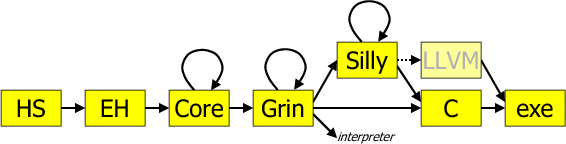
\includegraphics[scale=0.8]{ehc-dataflow2}
\caption{UHC pipeline}
\label{flow}
\end{figure}

For this thesis only the first two phases are interesting. The HS and the EH phases, which are reused:
\begin{description}
\item[\textbf{HS}] In the HS phase the concrete Haskell syntax is parsed into the abstract syntax. 
\item[\textbf{EH}] The Haskell syntax contains a lot of syntactic sugar. In the EH phase the abstract syntax is desugared and preprocessed.
\end{description}
\subsection{Variant}
UHC as indicated before is a series of smaller compilers. These different versions of the compiler are called \emph{variants}. A tool called \emph{shuffle} is used to weave these variants together. The variant used in this thesis is variant 8. This variant provides no code generation but does provide a parser, renamer, desugarer and typechecker which can be reused and partially overridden.

In terms of \emph{Haskell98} all the needed constructs are there except for \emph{type classes}. This variant is simple enough to be implemented in the alloted time, but complete enough that we can implement a large subset of Haskell functionality using it. Including higher-rank functions.

\subsection{EH}
The abstract language used by the Utrecht Haskell Compiler (UHC) to represent desugared Haskell is called Essential Haskell or EH for short. EH at its core resembles $\lambda-calculus$ but with added \textbf{Let} bindings. EH denotes a Haskell file but with all the syntactical sugar of the HS file removed, leaving only a core set of basic operations that need to be supported. EH will be further explored in chapter \ref{Implementation}.

\chapter{Attribute Grammars}
\label{AG}
\emph{Context Free Grammars}(CFG) can only describe the syntax of programming languages\cite{knuth1}. They cannot specify any context-sensitive conditions. In practice we are interested in more then the well-formedness of a grammar. For example the condition that the same value for \emph{n} be enforced in the string $a^nb^nc^n$ cannot be described by using context free grammars\cite{ken}.

In 1968 by Donald E. Knuth~\cite{knuth1} introduced \ags as a way to define the \emph{meaning} to context free languages. A typical is the defining the value of an expression. The expression grammar is defined by the following \emph{CFG} expressed as \emph{BNF}:

\begin{figure}[H]
\begin{grammar}
      [(colon){$\rightarrow$}]
      [(semicolon)$|$]
      [(comma){}]
      [(period){\\}]
      [(quote){\begin{bf}}{\end{bf}}]
      [(nonterminal){$\langle$}{$\rangle$}]
<Expr>   \hspace{52pt} : <number>; <Expr>, <operator>, <Expr>.
<number> \hspace{42pt} : <digit>;<digit>,<number>.
<digit> \hspace{55pt} : "0";"1";"2";"3";"4";"5";"6";"7";"8";"9".
<relational operator>: "$-$";"$+$".
\end{grammar}
\caption{BNF definition for Expressions}
\label{grammar:bnf:expr}
\end{figure}

A symbol is either a terminal or a nonterminal. A terminal is typically a single character or a single token. A nonterminal represents a sequence of symbols, and can be seen as a classification of these symbols.
The \emph{terminals} in this case are the \emph{operators} $+,-$ and the \emph{digits} $0\ldots 9$. The \emph{nonterminals} are the \emph{Expr} and \emph{number} symbols. The grammar specifies that an expression is either a \emph{number} or an \emph{Expr} followed by an \emph{operator} and then another \emph{Expr}. For every sentence that can be produced by this grammar a parse tree can be assigned. For instance, the expression "2 + (3 - 5) + (6 - 1)" produces the parse tree in figure \ref{fig.example1.parsetree}. We define the value of an expression as a composition of the values of its sub expressions, See figure \ref{fig.example1.parsetree}

\begin{figure}[H]
\centering
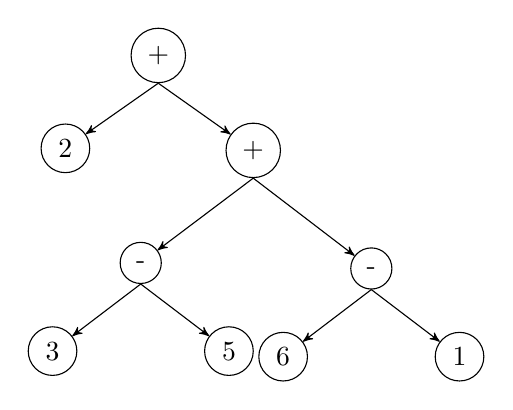
\begin{tikzpicture}[>=stealth']
\node (r0) [draw, circle] {+};
\node (r1) [below left=1cm of r0, draw, circle] {2}
  edge[<-] (r0.south);
\node (r2) [below right=1cm of r0, draw, circle] {+}
  edge[<-] (r0.south);
\node (s0) [below left=1.4cm of r2, draw, circle] {-}
  edge[<-] (r2.south);
\node (s1) [below left=1cm of s0, draw, circle] {3}
  edge[<-] (s0.south);
\node (s2) [below right=1cm of s0, draw, circle] {5}
  edge[<-] (s0.south);
\node (f0) [below right=1.5cm of r2, draw, circle] {-}
  edge[<-] (r2.south);
\node (f1) [below left=1cm of f0, draw, circle] {6}
  edge[<-] (f0.south);
\node (f2) [below right=1cm of f0, draw, circle] {1}
  edge[<-] (f0.south);
\end{tikzpicture}
\caption{Parse tree example for "2 + (3 - 5) + (6 - 1)"}
\label{fig.example1.parsetree}
\end{figure}

AG's are additions to CFGs that propagate semantic information along through parse trees. Nodes in the AST correspond to either a production or a nonterminal in the grammar. With this in mind there are two kinds of \emph{attributes} defined by knuth\cite{knuth1}:
\begin{description}
\item[\textbf{synthesized}] An attribute that is defined in terms of attributes of the \emph{descendants} of the AST node. They are passed bottom-up through the tree.
\item[\textbf{inherited}] An attribute that is defined in terms of the \emph{ancestors} of the nonterminal. They are passed top-down through the tree.
\end{description}

An attribute can be both \emph{synthesized} and \emph{inherited}. These are however different attributes which share the same name. Semantics can be defined for the tree in figure \ref{fig.example1.parsetree} by assigning a synthesized attribute named \emph{value} of type \textbf{Int} to the nonterminals \emph{number} and \emph{Expr}. The evaluation rules are:

\begin{figure}[H]
\begin{grammar}
      [(colon){$\rightarrow$}]
      [(semicolon)$|$]
      [(comma){}]
      [(period){\\}]
      [(quote){\begin{bf}}{\end{bf}}]
      [(nonterminal){$\langle$}{$\rangle$}] 
value(<$Expr^+$>) : value(<$Expr_1$>) + value(<$Expr_2$>). 
value(<$Expr^-$>) : value(<$Expr_1$>) - value(<$Expr_2$>). 
value(<Expr>) \hspace{5pt} : value(<number>).
value(<number>): <number>.
\end{grammar}
\caption{attribute definition for Expressions}
\label{semantics:bnf:expr}
\end{figure}

Subscripts disambiguate between the different expression types and superscripts  distinguish between the different cases of the \emph{operator} in an expression. Figure \ref{fig.example2.decoratedtree} shows a tree decorated with the synthesized attribute \emph{v} (short for value) along with intermediate values of \emph{v}.

\begin{figure}[H]
\centering
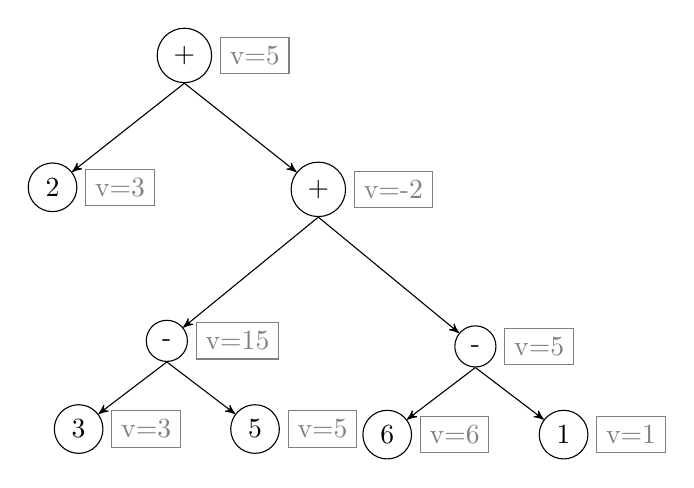
\begin{tikzpicture}[>=stealth']
\node (r0) [draw, circle] {+};
\node (ri0) [draw, rectangle, right=0.1cm of r0, gray] {v=5};
\node (r1) [below left=1.7cm of r0, draw, circle] {2}
  edge[<-] (r0.south);
\node (ri1) [draw, rectangle, right=0.1cm of r1, gray] {v=3};
\node (r2) [below right=1.7cm of r0, draw, circle] {+}
  edge[<-] (r0.south);
\node (ri2) [draw, rectangle, right=0.1cm of r2, gray] {v=-2};
\node (s0) [below left=2.1cm of r2, draw, circle] {-}
  edge[<-] (r2.south);
\node (ri3) [draw, rectangle, right=0.1cm of s0, gray] {v=15};
\node (s1) [below left=1.0cm of s0, draw, circle] {3}
  edge[<-] (s0.south);
\node (ri4) [draw, rectangle, right=0.1cm of s1, gray] {v=3};
\node (s2) [below right=1.0cm of s0, draw, circle] {5}
  edge[<-] (s0.south);
\node (ri5) [draw, rectangle, right=0.1cm of s2, gray] {v=5};
\node (f0) [below right=2.2cm of r2, draw, circle] {-}
  edge[<-] (r2.south);
\node (ri6) [draw, rectangle, right=0.1cm of f0, gray] {v=5};
\node (f1) [below left=1.0cm of f0, draw, circle] {6}
  edge[<-] (f0.south);
\node (ri7) [draw, rectangle, right=0.1cm of f1, gray] {v=6};
\node (f2) [below right=1.0cm of f0, draw, circle] {1}
  edge[<-] (f0.south);
\node (ri8) [draw, rectangle, right=0.1cm of f2, gray] {v=1};
\end{tikzpicture}
\caption{decorated tree example for "2 + (3 - 5) + (6 - 1)"}
\label{fig.example2.decoratedtree}
\end{figure}

\Ags are akin to \emph{catamorphisms}, except without the need to define the algebra and explicit traversals of the tree.

\section{Utrecht University Attribute Grammar Compiler (UUAGC)}
UUAGC (Utrecht University Attribute Grammar Compiler) is a preprocessor which parses Attribute Grammars in a custom language.
The grammar, attributes for nonterminals and rules for attributes per production can be specified in attribute grammar source code. The preprocessor translates the attribute grammar code to datatype declarations, folds and semantic functions, which are functions that assign meaning to the specified grammar. In the UHC Type checker, the UUAGC system is used to do most of the work, with the exception of unification.

\subsection{Limits of UUAGC}
The \emph{UUAGC} system is limited in that it cannot perform case distinctions over multiple \emph{abstract syntax trees} at the same time\cite{visitag}. For most applications this is not an issue, since in most cases there is only one \emph{AST} that needs to be traversed at a time. 

In an attribute grammar, we express a function between inherited and synthesized attributes. The productions form the cases of this function, and we give rules for each case. Thus, we distinguish cases based on the production. For some example, we wish to also distinguish cases based on attribute values. This we cannot express with conventional attribute grammars.

With higher-order AGs, it is possible to define a grammar for the call-tree of such a function. A higher-order attribute can then inspect the attribute's values and dispatch to a suitable production. However, this is a rather primitive mechanism to express case distinctions.

Unification is one such example where we need to distinguish cases based on attribute values. Unification is the act of trying to find structural \& semantic equivalence between two types. It is a critical part of type checking. Given two types \emph{$t_{1}$} and \emph{$t_{2}$}, unification attempts to find a list of substitutions that allows the instantiation of type \emph{$t_{1}$} to type \emph{$t_{2}$}. For this to be accomplished it needs to be possible to traverse both \emph{$t_{1}$} and \emph{$t_{2}$} concurrently; while comparing the types at every node.

%\begin{figure}[!h]
%\begin{center}
%\begin{neatopic}[width=.5\textwidth, height=50mm]
%    subgraph type1 {
%	  node [];
%	  a1 [label="a"];
%	  a2 [label="b"];
%	  a1 -- a2;
%	  label = "Type 1";
%    }
%
%    subgraph type1 {
%	  node [];
%	  b1 [label="Int"];
%	  b2 [label="Int"];
%        b1 -- b2;
%	  label = "Type 2";
%    }
%    
%    {rank=same; a1 b1}
%    {rank=same; a2 b2}
%
%    a1 -- b1 [style=dotted, label ="a:= Int"];
%    a2 -- b2 [style=dotted, label ="b:= Int"];
%\end{neatopic}
%\end{center}
%\caption{Unification example}
%\label{unify-simple}
%\end{figure}

When unifying the type \emph{$a \rightarrow b$} with \emph{$Int \rightarrow Int$} both trees are traversed concurrently while the nodes are compared, and ultimately terminating with the substitution list [(a,Int), (b, Int)]. The ability to be able to traverse \emph{AST}s that were just produced is also required because the structure of the \emph{type} being produced is not known beforehand. During type inference more type information is gradually gained on the type that needs to be produced. This generally presents a problem for AGs\cite{ruler-front} because the synthesis and evaluation phases are two separate phases.

\section{Ruler-Core}
\Rcore addresses these restrictions in AG by introducing a model based on \emph{visit}\cite{visits} functions. The resulting language is more flexible while still retaining the core semantics of reasoning over decorated trees with attributes. The simplest description of ruler-core would be:\emph{a language to manipulate visit sequences.}

\begin{quotation}
A \emph{visit function}\cite{visitag} is a (partial) function that takes several inputs (\emph{inherited attributes}) and produces several output values (\emph{synthesized attributes}) and a continuation for the next visit.
\end{quotation}

As with traditional AGs \emph{inherited}, attributes are passed top-down in the tree while \emph{synthesized} attributes are passed bottom-up. An attribute can be both \emph{synthesized} and \emph{inherited}.

Everything that can be expressed in uuagc can be expressed in ruler-core, but the inverse is not true. One of the simplest things that can be done in ruler-core is the evaluation of a single AST. In order to write an evaluator for the expression type in figure \ref{grammar:bnf:expr} we first need to define the \emph{datatypes} and \emph{interfaces}.

\begin{figure}[H]
\begin{minipage}[t]{0.4\linewidth}
\begin{hscode}\SaveRestoreHook
\column{B}{@{}>{\hspre}l<{\hspost}@{}}%
\column{3}{@{}>{\hspre}l<{\hspost}@{}}%
\column{5}{@{}>{\hspre}l<{\hspost}@{}}%
\column{13}{@{}>{\hspre}l<{\hspost}@{}}%
\column{16}{@{}>{\hspre}l<{\hspost}@{}}%
\column{E}{@{}>{\hspre}l<{\hspost}@{}}%
\>[B]{}\mathbf{data}\;\Conid{Expr}{}\<[E]%
\\
\>[B]{}\hsindent{3}{}\<[3]%
\>[3]{}\mathbf{con}\;\Conid{Num}\;{}\<[E]%
\\
\>[3]{}\hsindent{2}{}\<[5]%
\>[5]{}\Varid{val}{}\<[13]%
\>[13]{}\mathbin{::}\Conid{Int}{}\<[E]%
\\
\>[B]{}\hsindent{3}{}\<[3]%
\>[3]{}\mathbf{con}\;\Conid{Expr}\;{}\<[E]%
\\
\>[3]{}\hsindent{2}{}\<[5]%
\>[5]{}exp_1{}\<[13]%
\>[13]{}\mathbin{:}{}\<[16]%
\>[16]{}\Conid{Expr}{}\<[E]%
\\
\>[3]{}\hsindent{2}{}\<[5]%
\>[5]{}\Varid{op}{}\<[13]%
\>[13]{}\mathbin{::}\Conid{Operator}{}\<[E]%
\\
\>[3]{}\hsindent{2}{}\<[5]%
\>[5]{}exp_2{}\<[13]%
\>[13]{}\mathbin{:}{}\<[16]%
\>[16]{}\Conid{Expr}{}\<[E]%
\ColumnHook
\end{hscode}\resethooks
\end{minipage}
\begin{minipage}[t]{0.6\linewidth}
\begin{hscode}\SaveRestoreHook
\column{B}{@{}>{\hspre}l<{\hspost}@{}}%
\column{3}{@{}>{\hspre}l<{\hspost}@{}}%
\column{5}{@{}>{\hspre}l<{\hspost}@{}}%
\column{14}{@{}>{\hspre}l<{\hspost}@{}}%
\column{22}{@{}>{\hspre}l<{\hspost}@{}}%
\column{E}{@{}>{\hspre}l<{\hspost}@{}}%
\>[B]{}\mathbf{data}\;\Conid{Operator}{}\<[E]%
\\
\>[B]{}\hsindent{3}{}\<[3]%
\>[3]{}\mathbf{con}\;\Conid{Plus}{}\<[E]%
\\
\>[B]{}\hsindent{3}{}\<[3]%
\>[3]{}\mathbf{con}\;\Conid{Minus}{}\<[E]%
\\[\blanklineskip]%
\>[B]{}\mathbf{itf}\;\Conid{Expr}\;{}\<[E]%
\\
\>[B]{}\hsindent{3}{}\<[3]%
\>[3]{}\mathbf{visit}\;\Varid{eval}\;{}\<[E]%
\\
\>[3]{}\hsindent{2}{}\<[5]%
\>[5]{}\mathbf{inh}\;\Varid{ast}{}\<[14]%
\>[14]{}\mathbin{::}\Conid{Expr}\mbox{\onelinecomment  input}{}\<[E]%
\\
\>[3]{}\hsindent{2}{}\<[5]%
\>[5]{}\mathbf{syn}\;\Varid{v}{}\<[14]%
\>[14]{}\mathbin{::}\Conid{Int}{}\<[22]%
\>[22]{}\mbox{\onelinecomment  output}{}\<[E]%
\ColumnHook
\end{hscode}\resethooks
\end{minipage}
\caption{Evaluating expressions in ruler-core: datatypes}
\label{example:tutorial1:datatypes}
\end{figure}

\subsubsection{Data types}
\Rcore data types resemble Haskell's record syntax with some notable differences.

Instead of an $=$ or \textbar \space like in Haskell, an explicit \textbf{con} keyword is used to indicate the \emph{name} of the constructor. Every element of the constructor must be explicitly named. Indentation is also important since indentation separates constructors, in general \textbf{con} needs to be deeper indented then \textbf{data} and the members of a constructor should be indented further than the \textbf{con}. 

Figure \ref{example:tutorial1:datatypes} illustrates two different ways of declaring a type of constructor argument. $:$ is used to declare a type that is a \emph{nonterminal} and $::$ indicates a \emph{terminal}. The reason for this distinction is that for \emph{nonterminal} types some extra machinery is automatically defined. It is important to know that for every nonterminal \rcore enforces that at least one of the declared visits have an \emph{inherited} attribute named \emph{ast} with the type of the nonterminal.

Only types of kind $:: \star$ are allowed by \rcore, which means only monomorphic types are accepted. As is the case with UUAGC, the constructors generated will be in the form of \emph{TypeName\_ConstructorName}. To put this concretely figure \ref{example:tutorial1:datatypes} exposes for the type \emph{Expr} the constructor functions \textbf{Expr\_Num} and \textbf{Expr\_Expr}.

\subsection{Interfaces}
\emph{Interfaces} are analogous to the interface definitions in other languages, except instead of declaring function prototypes/signatures we declare visits and their attributes. Interfaces declare \emph{nonterminal}s which can be named the same as their corresponding \emph{data types}. For those familiar with uuagc, a \textbf{ATTR} declaration in uuagc would equal an interface declaration with one visit and all the attributes declared in the \textbf{ATTR} would be part of this one visit. The ability to explicitly declare these visits and interfaces is where ruler-core's true abilities come in.

\begin{figure}[h!]
\begin{hscode}\SaveRestoreHook
\column{B}{@{}>{\hspre}l<{\hspost}@{}}%
\column{3}{@{}>{\hspre}l<{\hspost}@{}}%
\column{5}{@{}>{\hspre}l<{\hspost}@{}}%
\column{E}{@{}>{\hspre}l<{\hspost}@{}}%
\>[B]{}\mathbf{itf}\mathbin{<}\Varid{name}\mathbin{>}{}\<[E]%
\\
\>[B]{}\hsindent{3}{}\<[3]%
\>[3]{}\{\mskip1.5mu \mathbf{visit}\mathbin{<}\Varid{name}\mathbin{>}{}\<[E]%
\\
\>[3]{}\hsindent{2}{}\<[5]%
\>[5]{}\{\mskip1.5mu \Varid{attributes}\mskip1.5mu\}{}\<[E]%
\\
\>[B]{}\hsindent{3}{}\<[3]%
\>[3]{}\mskip1.5mu\}{}\<[E]%
\ColumnHook
\end{hscode}\resethooks
\caption{Ruler-core interface declaration syntax}
\label{itf:syntax}
\end{figure}

Multiple visits can be defined for an interface. The order of appearance of visits is relevant. Every visit is a new \emph{co-routine} and will be scheduled to run by \rcore. The order of appearance of visits is relevant. Attributes that belong to an earlier visit are computed before attributes of a later visit. Visits are usually executed as soon as possible and as many visits as possible are executed at the same time. % Outside of visits we can also declare attributes. These attributes are thus not explicitly assigned to a visit. They will be automatically assigned to the earliest visit possible.

\subsection{Semantics}
We define the rules of a production per visit. A rule may only be applied in the same visit or a later visit than it is declared in. Also, visits introduce a scope.
Rules in \rcore are either an assertion (like a match statement), an assignment (assignment to attributes) or a statement (default rules, invocations, child declarations, etc..)

There are two kind of visits, one being the visits declared inside an interface and the other the visits declared in a semantic function. These are separate concepts. The visits of an interface declares what we want to compute and those of a semantic function declares how we want to compute these values.

Furthermore, a semantic visit is divided in one or more clauses. Each clause provides an alternative set of rules for the that visit of the production. During evaluation, clauses are tried in the order of appearance. Special match rules specify conditions for backtracking.
In ruler-core, productions themselves are actually also clauses.

Interface visits like all functions have arguments, or in this case attributes. The \emph{inh} keyword indicates an \emph{inherited} attribute (input value), whereas \emph{syn} indicates a \emph{synthesized} attribute (output value). The order of declaration of the attributes is not important.

After declaring the datatypes and interfaces; the actual semantic function can be declared to evaluate the expressions:

\begin{figure}[H]
\begin{hscode}\SaveRestoreHook
\column{B}{@{}>{\hspre}l<{\hspost}@{}}%
\column{4}{@{}>{\hspre}l<{\hspost}@{}}%
\column{6}{@{}>{\hspre}l<{\hspost}@{}}%
\column{8}{@{}>{\hspre}l<{\hspost}@{}}%
\column{10}{@{}>{\hspre}l<{\hspost}@{}}%
\column{E}{@{}>{\hspre}l<{\hspost}@{}}%
\>[B]{}\mathbf{datasem}\;\Conid{Expr}\;{}\<[E]%
\\
\>[B]{}\hsindent{4}{}\<[4]%
\>[4]{}\mathbf{clause}\;\Conid{Num}\;{}\<[E]%
\\
\>[4]{}\hsindent{2}{}\<[6]%
\>[6]{}\mathbf{lhs}\mbox{.}\Varid{v}\mathrel{=}\mathbf{loc}\mbox{.}\Varid{val}\mbox{\onelinecomment  output}{}\<[E]%
\\
\>[B]{}\hsindent{4}{}\<[4]%
\>[4]{}\mathbf{clause}\;\Conid{Expr}\;{}\<[E]%
\\
\>[4]{}\hsindent{2}{}\<[6]%
\>[6]{}\mathbf{internal}\;\Varid{opcheck}\;{}\<[E]%
\\
\>[6]{}\hsindent{2}{}\<[8]%
\>[8]{}\mathbf{clause}\;\Conid{Plus}\;{}\<[E]%
\\
\>[8]{}\hsindent{2}{}\<[10]%
\>[10]{}\mathbf{match}\;\Conid{\Conid{Operator}.Plus}\mathord{@}\mathbf{loc}\mathrel{=}\mathbf{loc}\mbox{.}\Varid{op}{}\<[E]%
\\
\>[8]{}\hsindent{2}{}\<[10]%
\>[10]{}\mathbf{lhs}\mbox{.}\Varid{v}\mathrel{=}exp_1\mbox{.}\Varid{v}\mathbin{+}exp_2\mbox{.}\Varid{v}\mbox{\onelinecomment  output}{}\<[E]%
\\
\>[6]{}\hsindent{2}{}\<[8]%
\>[8]{}\mathbf{clause}\;\Conid{Minus}\;{}\<[E]%
\\
\>[8]{}\hsindent{2}{}\<[10]%
\>[10]{}\mathbf{match}\;\Conid{\Conid{Operator}.Minus}\mathord{@}\mathbf{loc}\mathrel{=}\mathbf{loc}\mbox{.}\Varid{op}{}\<[E]%
\\
\>[8]{}\hsindent{2}{}\<[10]%
\>[10]{}\mathbf{lhs}\mbox{.}\Varid{v}\mathrel{=}exp_1\mbox{.}\Varid{v}\mathbin{-}exp_2\mbox{.}\Varid{v}\mbox{\onelinecomment  output}{}\<[E]%
\ColumnHook
\end{hscode}\resethooks
\caption{Evaluating expressions in ruler-core: datasem}
\label{example:tutorial1:datasem}
\end{figure}

The elements that are part of figure \ref{example:tutorial1:datasem} will be explained in the coming sections:

\subsection{Semantic functions}
\label{semantics}
A semantic function is a function that defines a semantic for a interface. % Within a semantic function it is possible to \emph{invoke} any other coroutine(s) that might be needed. Although there is an implicit \textbf{invoke} keyword, it is rarely needed to explicitly \emph{invoke} a visit. When all attributes are defined for a visit it is implicitly invoked.

The contents of a semantic function is formed by rules. Rules are given per production, per visit and per clause. Rules exists in several form. Clauses provide a way to do scoping inside semantic functions. A clause inherits all the attributes of its parent clauses in the same visit. If a visit has only one clause it does not have to be explicitly declared. 

There are two ways of defining a semantic function: using the \textbf{datasem} and a \textbf{sem} keyword. The example in figure \ref{example:tutorial1:datasem} uses the former.

\subsubsection{Datasem}
Defining semantics for a \emph{data type} and \emph{nonterminal}(interface) defined in \rcore can be done with a shorthand: \textbf{datasem}. As the name suggests \textbf{datasem} stands for \emph{datatype semantics}. % Those familiar with uuagc can compare defining a \textbf{datasem} in \rcore with a \textbf{SEM} declaration in uuagc.

\begin{figure}[!h]
\begin{hscode}\SaveRestoreHook
\column{B}{@{}>{\hspre}l<{\hspost}@{}}%
\column{5}{@{}>{\hspre}l<{\hspost}@{}}%
\column{9}{@{}>{\hspre}c<{\hspost}@{}}%
\column{9E}{@{}l@{}}%
\column{E}{@{}>{\hspre}l<{\hspost}@{}}%
\>[B]{}\mathbf{datasem}\mathbin{<}\Varid{nonterminal}\mathbin{>}[\mskip1.5mu \Varid{monad}\mathbin{<}\mathbf{type}\mathbin{>}\mskip1.5mu]{}\<[E]%
\\
\>[B]{}\hsindent{5}{}\<[5]%
\>[5]{}\{\mskip1.5mu \mathbf{clause}\mathbin{<}\Varid{name}\mathbin{>}{}\<[E]%
\\
\>[5]{}\hsindent{4}{}\<[9]%
\>[9]{}\mathbin{...}{}\<[9E]%
\\
\>[B]{}\hsindent{5}{}\<[5]%
\>[5]{}\mskip1.5mu\}{}\<[E]%
\ColumnHook
\end{hscode}\resethooks
\caption{Syntax definition of a sem function}
\label{datasem:syntax}
\end{figure}

Defining a \textbf{datasem} is a shorthand for defining a \textbf{sem} (more on this later). The \emph{monad} type is optional and will be ignored for now. %, however if a type was specified for any semantic function which is used by, or used in this \textbf{datasem} then to disambiguate you need to define the type in this declaration as well.

The \emph{clauses} in a \textbf{datasem} should coincide with the constructors of the data type. The preprocessor enforces that there is a clause for every declared constructor. Every clause declaration implicitly adds a \textbf{match} statement for every clause. This is the reason why there is a required attribute \emph{ast} for ever nonterminal. This is the attribute on which matches are tried out on in the main clauses of a \textbf{datasem}. A \textbf{match} is essentially an assertion, if failed nothing else for that clause is tried out and backtracking takes place.

For every \textbf{datasem}, in every clause where there is a nonterminal in the definition of that clause, there will be an implicit child declared for that field. It is for this reason that in figure \ref{example:tutorial1:datasem} it is refered to the operator terminal via the local child (loc.op) and the \emph{\ensuremath{exp_1}} and \emph{\ensuremath{exp_2}} nonterminals directly. In the case of \emph{Expr} there was only one \emph{inherited} attribute: ast, but since ast is filled in automatically by \rcore the invoke is implicitly performed. Which is why the synthesized attributes can be accessed without any further action. 

Because of all these properties, a \textbf{datasem} only provides the ability to traverse one tree at a time.
\subsection{Bindings}
\label{bindings}
In Haskell the \emph{Let} binding is used when introducing new variables in a sequential computation. In \rcore the keyword \textbf{let} is not used when assigning values to bindings, however since bindings in \rcore are translated to \textbf{let} declarations by the preprocessor the same behaviors is to expected. This means that binding to a \emph{pattern} on the \emph{left hand side} is valid. e.g. \[ (\alpha, \beta) = \ldots \] is allowed. This allows the definition multiple attributes at the same time.

An attribute may only be defined once. The compiler will generate an error if it finds code that tries to redefine an attribute (there is no shadowing).

The notation for referencing patterns, expressions and variables is \emph{k}.\emph{x} where \emph{k} is the name of child name and \emph{x} the attribute to be referenced. There are two build in reserved children:

\paragraph{lhs}
The \emph{lhs} child is used to access the \emph{inherited} attributes and to assign values to the \emph{synthesized} attributes. Which one is intended is derived from the context in which they are used: When used at the \emph{left hand side} of an expression they are treated as \emph{synthesized} attributes, but when used in the \emph{right hand side} of a binding they refer to the \emph{inherited} values.
 
\paragraph{loc}
The \emph{loc} child is used in a way that is analogous to local variables in other languages. As many \emph{loc} attributes as needed can be defined. The scope of the \emph{loc} is only the clause/visit that it is declared in and the its children.

\subsection{Clauses}
Clauses are a way of defining alternatives. When an assertion in clause fails  it backtracks out of the clause and the next one is tried out. Clauses are tried out in sequential order. A visit can contain multiple clauses, corresponding to the different ways to interpret the \emph{inherited} attributes of the visit.

If no clause can be executed in a visit, the system backtracks to the parent visit and clause. This behavior goes all the way up to the root. In order to be able to generate proper errors it is recommended to always make the collection of clauses for a visit total. The easiest way to do this is to make a \emph{catch-all} clause at the end.

\subsection{Matches}
Matches are akin to case expressions, like case expressions they force evaluation and attempt to pattern match on the datatype. Except unlike case expressions, you can only on a pattern that contains a constructor. For any data type defined in \rcore itself and the \emph{Bool} type a \textbf{match} can be done.

\begin{figure}[h!]
\begin{hscode}\SaveRestoreHook
\column{B}{@{}>{\hspre}l<{\hspost}@{}}%
\column{39}{@{}>{\hspre}l<{\hspost}@{}}%
\column{E}{@{}>{\hspre}l<{\hspost}@{}}%
\>[B]{}\mathbf{match}\;\Conid{\Conid{TypeName}.ConstructorName}\mathord{@}\mathbf{child}{}\<[39]%
\>[39]{}\mathrel{=}\mathbin{<}\Varid{expression}\mathbin{>}{}\<[E]%
\ColumnHook
\end{hscode}\resethooks
\caption{Match syntax definition}
\label{match:syntax}
\end{figure}

If the \emph{match} succeeds the \emph{named} attributes defined for the elements of the Constructor are added as attributes of the specified \emph{child}. Of the two reserved children \textbf{lhs} and \textbf{loc} only \textbf{lhs} is not allowed as a child name here\footnote{note that the childname "var" is also reserved, but in the case of var you will get an actual syntax error}. On the other hand if the \emph{match} fails the entire clause is aborted and backtracking is performed.
There are exceptions to this syntax, \emph{build in} types such as \emph{Bool} which have no children have an alternative syntax:

\begin{figure}[h!]
\begin{hscode}\SaveRestoreHook
\column{B}{@{}>{\hspre}l<{\hspost}@{}}%
\column{E}{@{}>{\hspre}l<{\hspost}@{}}%
\>[B]{}\mathbf{match}\;\Conid{True}\mathrel{=}\mathbin{<}\Varid{expression}\mathbin{>}{}\<[E]%
\ColumnHook
\end{hscode}\resethooks
\caption{Example match on Bools}
\label{match:bool}
\end{figure}

Figure \ref{match:bool} shows that on certain types the rules are relaxed, particularly the Bool type. Note that because there is no build in support for the \emph{Maybe} type, often in this thesis this will be supported by first match on \ensuremath{\Conid{True}\mathrel{=}\Varid{isJust}\;\Varid{expr}} and then a subsequent call the \ensuremath{\Varid{fromJust}} function.

\subsection{Internal}
Sometimes it is necessary to branch on a value that was just synthesized. This is achieved by using the \emph{internal} keyword. The \emph{internal} keyword provides a means of scoping and branching at the same time. Internals contain a list of \emph{clauses} which will be tried out in order one at a time. Attributes that were declared before the \emph{internal} statement are all in scope inside an internal block. 

\begin{figure}[h!]
\begin{hscode}\SaveRestoreHook
\column{B}{@{}>{\hspre}l<{\hspost}@{}}%
\column{3}{@{}>{\hspre}l<{\hspost}@{}}%
\column{E}{@{}>{\hspre}l<{\hspost}@{}}%
\>[B]{}\mathbf{internal}\mathbin{<}\Varid{name}\mathbin{>}{}\<[E]%
\\
\>[B]{}\hsindent{3}{}\<[3]%
\>[3]{}\{\mskip1.5mu \mathbf{clause}\mskip1.5mu\}{}\<[E]%
\\
\>[B]{}\hsindent{3}{}\<[3]%
\>[3]{}\{\mskip1.5mu \mathbf{clause}\mskip1.5mu\}{}\<[E]%
\\
\>[B]{}\hsindent{3}{}\<[3]%
\>[3]{}\mathbin{...}{}\<[E]%
\ColumnHook
\end{hscode}\resethooks
\caption{Internal syntax definition}
\label{internal:syntax}
\end{figure}

A clause may have at most one internal visit, although an internal visit may have clauses with again an internal visit.  Any code below the internal is floated upward if possible. Referencing a attribute defined in an internal from a parent clause is invalid.

\subsection{Invoking semantic functions}
\label{calling:sem}
To complete this example we also need be able to call semantic functions from Haskell:

\begin{figure}[H]
\begin{hscode}\SaveRestoreHook
\column{B}{@{}>{\hspre}l<{\hspost}@{}}%
\column{3}{@{}>{\hspre}l<{\hspost}@{}}%
\column{E}{@{}>{\hspre}l<{\hspost}@{}}%
\>[B]{}\Varid{eval}\mathbin{::}\Conid{Expr}\to \Conid{IO}\;\Conid{Int}{}\<[E]%
\\
\>[B]{}\Varid{eval}\;\Varid{exp}\mathrel{=}\mathbf{do}{}\<[E]%
\\
\>[B]{}\hsindent{3}{}\<[3]%
\>[3]{}\mathbf{let}\;\mathbf{inh}\mathrel{=}\Conid{Inh\char95 Expr\char95 eval}\;\{\mskip1.5mu \Varid{ast\char95 Inh\char95 Expr}\mathrel{=}\Varid{exp}\mskip1.5mu\}{}\<[E]%
\\
\>[B]{}\hsindent{3}{}\<[3]%
\>[3]{}\mathbf{syn}\leftarrow \Varid{invoke\char95 Expr\char95 eval}\;\Varid{dnt\char95 Expr}\;\mathbf{inh}{}\<[E]%
\\
\>[B]{}\hsindent{3}{}\<[3]%
\>[3]{}\mathbf{let}\;\Varid{x}\mathrel{=}\Varid{v\char95 Syn\char95 Expr}\;\mathbf{syn}{}\<[E]%
\\
\>[B]{}\hsindent{3}{}\<[3]%
\>[3]{}\Varid{return}\;\Varid{x}{}\<[E]%
\ColumnHook
\end{hscode}\resethooks
\caption{calling wrappers from within haskell}
\end{figure}

The first line (the let) defines the \emph{inherited} attributes expected for the visit that is to be called. In this case the \emph{eval} visit, which specified that there is one \emph{inherited} attribute called \emph{ast}. For every visit there is a record for the \emph{inherited} and \emph{synthesized} attributes. The record name is build up as \textbf{X\_I\_v} where \textbf{X} equals "Inh" or "Syn", \textbf{I} is the interface name and \textbf{v} the visit name.

The labels of the fields inside these record are made up of \textbf{attr\_X\_I} where \textbf{attr} is the attribute name, \textbf{X} either "Inh" or "Syn" indicating the attribute type and \textbf{I} the interface name.

The second line invokes the \textbf{eval} routine with the given \emph{inherited} attributes and returns the \emph{synthesized} attribute records. The syntax for invoking a visit is \textbf{invoke\_I\_v \emph{wrapper inhs}}. The \textbf{I} indicates the interface name, the \textbf{v} the visit name, \textbf{inhs} stands for the record containing the inherited attributes and finally \textbf{wrapper} is the wrapper function to call. For every \textbf{datasem} \rcore defines a wrapper \textbf{dnt\_I} and for every \textbf{sem} function the name which was explicitly given is used (more on this later).

The expression example can be scaled up by adding variables to the expressions. Two extra constructors need to be introduced to \emph{Expr}. They correspond to introduction and elimination:	

\begin{hscode}\SaveRestoreHook
\column{B}{@{}>{\hspre}l<{\hspost}@{}}%
\column{3}{@{}>{\hspre}l<{\hspost}@{}}%
\column{5}{@{}>{\hspre}l<{\hspost}@{}}%
\column{13}{@{}>{\hspre}l<{\hspost}@{}}%
\column{16}{@{}>{\hspre}l<{\hspost}@{}}%
\column{E}{@{}>{\hspre}l<{\hspost}@{}}%
\>[3]{}\mathbf{con}\;\Conid{Var}\;{}\<[E]%
\\
\>[3]{}\hsindent{2}{}\<[5]%
\>[5]{}\Varid{nm}{}\<[13]%
\>[13]{}\mathbin{::}\Conid{String}{}\<[E]%
\\
\>[3]{}\mathbf{con}\;\Conid{Let}\;{}\<[E]%
\\
\>[3]{}\hsindent{2}{}\<[5]%
\>[5]{}\Varid{nm}{}\<[13]%
\>[13]{}\mathbin{::}\Conid{String}{}\<[E]%
\\
\>[3]{}\hsindent{2}{}\<[5]%
\>[5]{}\Varid{exp}{}\<[13]%
\>[13]{}\mathbin{:}{}\<[16]%
\>[16]{}\Conid{Expr}{}\<[E]%
\\
\>[3]{}\hsindent{2}{}\<[5]%
\>[5]{}\Varid{body}{}\<[13]%
\>[13]{}\mathbin{:}{}\<[16]%
\>[16]{}\Conid{Expr}{}\<[E]%
\ColumnHook
\end{hscode}\resethooks

In order to be able to evaluate variables an \emph{environment} needs to be passed down through the tree to collect all the declarations. This is done by modifying the \emph{interface} of \emph{Expr}. The new \emph{interface} definition is:

\begin{hscode}\SaveRestoreHook
\column{B}{@{}>{\hspre}l<{\hspost}@{}}%
\column{3}{@{}>{\hspre}l<{\hspost}@{}}%
\column{5}{@{}>{\hspre}l<{\hspost}@{}}%
\column{14}{@{}>{\hspre}l<{\hspost}@{}}%
\column{E}{@{}>{\hspre}l<{\hspost}@{}}%
\>[B]{}\mathbf{itf}\;\Conid{Expr}\;{}\<[E]%
\\
\>[B]{}\hsindent{3}{}\<[3]%
\>[3]{}\mathbf{visit}\;\Varid{eval}\;{}\<[E]%
\\
\>[3]{}\hsindent{2}{}\<[5]%
\>[5]{}\mathbf{inh}\;\Varid{ast}{}\<[14]%
\>[14]{}\mathbin{::}\Conid{Expr}{}\<[E]%
\\
\>[3]{}\hsindent{2}{}\<[5]%
\>[5]{}\mathbf{inh}\;\Varid{env}{}\<[14]%
\>[14]{}\mathbin{::}\Conid{Env}{}\<[E]%
\\
\>[3]{}\hsindent{2}{}\<[5]%
\>[5]{}\mathbf{syn}\;\Varid{v}{}\<[14]%
\>[14]{}\mathbin{::}\Conid{Int}{}\<[E]%
\\
\>[3]{}\hsindent{2}{}\<[5]%
\>[5]{}\mathbf{syn}\;\Varid{env}{}\<[14]%
\>[14]{}\mathbin{::}\Conid{Env}{}\<[E]%
\ColumnHook
\end{hscode}\resethooks

A new attribute \emph{env} is added which is both a \emph{synthesized} and \emph{inherited} attribute. Strictly speaking the \emph{env} can only be an \emph{inherited} attribute, however we allow access to variables introduced in the left branch in Expr in the right branch. In other words we allow the definition of variable in the left branch to be used in the right branch, which is why \emph{env} has to be synthesized as well.

Now that the type and interface have been updated, the next step is to extend the datatype semantics to support the new clauses.

\begin{hscode}\SaveRestoreHook
\column{B}{@{}>{\hspre}l<{\hspost}@{}}%
\column{4}{@{}>{\hspre}l<{\hspost}@{}}%
\column{6}{@{}>{\hspre}l<{\hspost}@{}}%
\column{15}{@{}>{\hspre}l<{\hspost}@{}}%
\column{16}{@{}>{\hspre}l<{\hspost}@{}}%
\column{E}{@{}>{\hspre}l<{\hspost}@{}}%
\>[4]{}\mathbf{clause}\;\Conid{Var}\;{}\<[E]%
\\
\>[4]{}\hsindent{2}{}\<[6]%
\>[6]{}\mathbf{loc}\mbox{.}\Varid{val}{}\<[15]%
\>[15]{}\mathrel{=}\Varid{lookup}\;\mathbf{loc}\mbox{.}\Varid{nm}\;\mathbf{lhs}\mbox{.}\Varid{env}{}\<[E]%
\\
\>[4]{}\hsindent{2}{}\<[6]%
\>[6]{}\mathbf{lhs}\mbox{.}\Varid{v}{}\<[15]%
\>[15]{}\mathrel{=}\Varid{fromMaybe}\;(\Varid{error}\mathbin{...})\;\mathbf{loc}\mbox{.}\Varid{val}{}\<[E]%
\\
\>[4]{}\mathbf{clause}\;\Conid{Let}\;{}\<[E]%
\\
\>[4]{}\hsindent{2}{}\<[6]%
\>[6]{}\mathbf{loc}\mbox{.}\Varid{env}{}\<[16]%
\>[16]{}\mathrel{=}(\mathbf{loc}\mbox{.}\Varid{nm},\Varid{exp}\mbox{.}\Varid{v})\mathbin{:}\mathbf{lhs}\mbox{.}\Varid{env}{}\<[E]%
\\
\>[4]{}\hsindent{2}{}\<[6]%
\>[6]{}\Varid{body}\mbox{.}\Varid{env}{}\<[16]%
\>[16]{}\mathrel{=}\mathbf{loc}\mbox{.}\Varid{env}{}\<[E]%
\\
\>[4]{}\hsindent{2}{}\<[6]%
\>[6]{}\mathbf{lhs}\mbox{.}\Varid{v}{}\<[16]%
\>[16]{}\mathrel{=}\Varid{body}\mbox{.}\Varid{v}{}\<[E]%
\ColumnHook
\end{hscode}\resethooks

The code for \ensuremath{\Conid{Var}} and \ensuremath{\Conid{Let}} show that \ensuremath{\mathbf{lhs}} is used both for synthesized and inherited attributes. Which is intended is determined by the way it is used (see section \ref{bindings}).

Sometimes special types such as Lists are needed. The next example shows how list support is provided in \rcore by adding the ability to evaluate a list of expressions.

\subsection{Special types}
At the time of writing \rcore only supports \emph{List}s in the category of special types, but can easily be extended to support any product datatype like \ensuremath{\Conid{Maybe}} and \ensuremath{\Conid{Map}}.

\subsubsection{Lists}
Lists are declared using the \textbf{type} keyword. The syntax is very familiar to Haskell programmer: \[ \textbf{type} \hspace{5pt} \emph{name} : [\emph{type}] \]

Declaring the list type \emph{Expr} would look like:

\begin{figure}[H]
\begin{hscode}\SaveRestoreHook
\column{B}{@{}>{\hspre}l<{\hspost}@{}}%
\column{E}{@{}>{\hspre}l<{\hspost}@{}}%
\>[B]{}\mathbf{type}\;\Conid{Exprs}\mathbin{:}[\mskip1.5mu \Conid{Expr}\mskip1.5mu]{}\<[E]%
\ColumnHook
\end{hscode}\resethooks
\caption{Exprs declaration using a list type}
\label{type:exprs}
\end{figure}

Figure \ref{type:exprs} declares the \emph{nonterminal} Exprs. This definition is semantically almost equivalent the data declaration in figure \ref{type:lists}. It introduces two type constructors \emph{Nil} and \emph{Cons} along with some extra attributes.

\begin{figure}[H]
\begin{hscode}\SaveRestoreHook
\column{B}{@{}>{\hspre}l<{\hspost}@{}}%
\column{3}{@{}>{\hspre}l<{\hspost}@{}}%
\column{5}{@{}>{\hspre}l<{\hspost}@{}}%
\column{9}{@{}>{\hspre}l<{\hspost}@{}}%
\column{E}{@{}>{\hspre}l<{\hspost}@{}}%
\>[B]{}\mathbf{data}\;\Conid{Exprs}{}\<[E]%
\\
\>[B]{}\hsindent{3}{}\<[3]%
\>[3]{}\mathbf{con}\;\Conid{Nil}{}\<[E]%
\\
\>[B]{}\hsindent{3}{}\<[3]%
\>[3]{}\mathbf{con}\;\Conid{Cons}\;{}\<[E]%
\\
\>[3]{}\hsindent{2}{}\<[5]%
\>[5]{}\Varid{hd}{}\<[9]%
\>[9]{}\mathbin{:}\Conid{Expr}{}\<[E]%
\\
\>[3]{}\hsindent{2}{}\<[5]%
\>[5]{}\Varid{tl}{}\<[9]%
\>[9]{}\mathbin{:}\Conid{Exprs}{}\<[E]%
\ColumnHook
\end{hscode}\resethooks
\caption{Syntactically equivalent definition of the Exprs type}
\label{type:lists}
\end{figure}

Next to creating the syntactical information, ruler-core also generates some \emph{Interface} declarations for every list type. 

The interface declared for the \emph{Exprs} example in figure \ref{type:lists} is equivalent to:

\begin{figure}[h!]
\begin{hscode}\SaveRestoreHook
\column{B}{@{}>{\hspre}l<{\hspost}@{}}%
\column{3}{@{}>{\hspre}l<{\hspost}@{}}%
\column{5}{@{}>{\hspre}l<{\hspost}@{}}%
\column{E}{@{}>{\hspre}l<{\hspost}@{}}%
\>[B]{}\mathbf{itf}\;\Conid{Exprs}\;{}\<[E]%
\\
\>[B]{}\hsindent{3}{}\<[3]%
\>[3]{}\mathbf{visit}\;\Varid{exprs\char95 visit}\;{}\<[E]%
\\
\>[3]{}\hsindent{2}{}\<[5]%
\>[5]{}\mathbf{inh}\;\Varid{ast}\mathbin{::}\Conid{Exprs}{}\<[E]%
\ColumnHook
\end{hscode}\resethooks
\caption{Ruler-core interface declaration syntax}
\label{itf:exprs}
\end{figure}

A special \emph{inherited} attribute \textbf{ast} is declared on which \emph{matches} will be performed in clauses. This interface itself is not useful, instead the preprocessor enforces that at least one of the visits declared for the \emph{non-terminal} Exprs contain an inherited attribute \emph{ast}. If this is not the case an error will be generated.

With figure \ref{type:lists} and \ref{itf:exprs} in mind the real interface to our \emph{Exprs} type can be declared along with the corresponding \textbf{datasem}.

\begin{figure}
\begin{minipage}[t]{0.4\linewidth}
\begin{hscode}\SaveRestoreHook
\column{B}{@{}>{\hspre}l<{\hspost}@{}}%
\column{3}{@{}>{\hspre}l<{\hspost}@{}}%
\column{5}{@{}>{\hspre}l<{\hspost}@{}}%
\column{14}{@{}>{\hspre}l<{\hspost}@{}}%
\column{E}{@{}>{\hspre}l<{\hspost}@{}}%
\>[B]{}\mathbf{itf}\;\Conid{Exprs}\;{}\<[E]%
\\
\>[B]{}\hsindent{3}{}\<[3]%
\>[3]{}\mathbf{visit}\;\Varid{eval}\;{}\<[E]%
\\
\>[3]{}\hsindent{2}{}\<[5]%
\>[5]{}\mathbf{inh}\;\Varid{ast}{}\<[14]%
\>[14]{}\mathbin{::}\Conid{Exprs}{}\<[E]%
\\
\>[3]{}\hsindent{2}{}\<[5]%
\>[5]{}\mathbf{inh}\;\Varid{env}{}\<[14]%
\>[14]{}\mathbin{::}\Conid{Env}{}\<[E]%
\\
\>[3]{}\hsindent{2}{}\<[5]%
\>[5]{}\mathbf{syn}\;\Varid{v}{}\<[14]%
\>[14]{}\mathbin{::}[\mskip1.5mu \Conid{Int}\mskip1.5mu]{}\<[E]%
\\
\>[3]{}\hsindent{2}{}\<[5]%
\>[5]{}\mathbf{syn}\;\Varid{env}{}\<[14]%
\>[14]{}\mathbin{::}\Conid{Env}{}\<[E]%
\ColumnHook
\end{hscode}\resethooks
\end{minipage}
\begin{minipage}[t]{0.6\linewidth}
\begin{hscode}\SaveRestoreHook
\column{B}{@{}>{\hspre}l<{\hspost}@{}}%
\column{4}{@{}>{\hspre}l<{\hspost}@{}}%
\column{6}{@{}>{\hspre}l<{\hspost}@{}}%
\column{15}{@{}>{\hspre}l<{\hspost}@{}}%
\column{E}{@{}>{\hspre}l<{\hspost}@{}}%
\>[B]{}\mathbf{datasem}\;\Conid{Exprs}\;{}\<[E]%
\\
\>[B]{}\hsindent{4}{}\<[4]%
\>[4]{}\mathbf{clause}\;\Conid{Cons}\;{}\<[E]%
\\
\>[4]{}\hsindent{2}{}\<[6]%
\>[6]{}\Varid{hd}\mbox{.}\Varid{env}{}\<[15]%
\>[15]{}\mathrel{=}\mathbf{lhs}\mbox{.}\Varid{env}{}\<[E]%
\\
\>[4]{}\hsindent{2}{}\<[6]%
\>[6]{}\Varid{tl}\mbox{.}\Varid{env}{}\<[15]%
\>[15]{}\mathrel{=}\mathbf{lhs}\mbox{.}\Varid{env}{}\<[E]%
\\
\>[4]{}\hsindent{2}{}\<[6]%
\>[6]{}\mathbf{lhs}\mbox{.}\Varid{v}{}\<[15]%
\>[15]{}\mathrel{=}\Varid{hd}\mbox{.}\Varid{v}\mathbin{:}\Varid{tl}\mbox{.}\Varid{v}{}\<[E]%
\\
\>[4]{}\hsindent{2}{}\<[6]%
\>[6]{}\mathbf{lhs}\mbox{.}\Varid{env}{}\<[15]%
\>[15]{}\mathrel{=}\mathbf{lhs}\mbox{.}\Varid{env}{}\<[E]%
\\
\>[B]{}\hsindent{4}{}\<[4]%
\>[4]{}\mathbf{clause}\;\Conid{Nil}\;{}\<[E]%
\\
\>[4]{}\hsindent{2}{}\<[6]%
\>[6]{}\mathbf{lhs}\mbox{.}\Varid{env}{}\<[15]%
\>[15]{}\mathrel{=}\mathbf{lhs}\mbox{.}\Varid{env}{}\<[E]%
\\
\>[4]{}\hsindent{2}{}\<[6]%
\>[6]{}\mathbf{lhs}\mbox{.}\Varid{v}{}\<[15]%
\>[15]{}\mathrel{=}[\mskip1.5mu \mskip1.5mu]{}\<[E]%
\ColumnHook
\end{hscode}\resethooks
\end{minipage}
\end{figure}

A lot of time is spent just copying over the \emph{env} attribute without actually doing anything with it. The larger the program gets the more problematic this becomes. For that \rcore has a mechanism called default rules.

\subsection{Default rules}
Default rules are a way of specifying default values for attributes that will be used in case explicit values are not given for the attributes in question. This is particularly useful for when it is required to do nothing in some clauses.
When using a \emph{default} rule, all the visits of all the children of the current production/node become active. This means every \emph{inherited} attribute must be filled in.
These rules are for both \emph{inherited} and \emph{synthesized} attributes. In case an attribute is both then the rule applies to both. 

Default rules collect values of attributes with the same name as the name for which the rule was declared. The values are collected in order of appearance. The \emph{head} of the list contains the value of the \emph{lhs} attribute (if it exists) and the \emph{tail} of the list contains the value of the last child. There are two kinds of \emph{default} rules:
\begin{description}
\item[\textbf{default}] { The \textbf{default} keyword generates a static error when none of the children of an attribute for which the rule is defined for return a result. }
\item[\textbf{default?}] { The \textbf{default?} returns the empty list instead of an exception when no child has the \emph{synthesized} attribute in mention. For \emph{inherited} attributes, the initial value \emph{lhs.attribute} is also added to the list. }
\end{description}

\begin{figure}[h!]
\[
\textbf{default[\textit{?}]} \hspace{5pt} \emph{attribute} = \emph{function}
\]
\caption{Syntax for default expressions}
\label{default:syntax}
\end{figure}

The default rules look at the attribute names and not the types. If a child defines an attribute for which there is a \emph{default} rule defined but where the \emph{type} of this attribute is different then the type of the other element of the list, then a type error will be generated by the Haskell compiler since Haskell lists are homogeneous.

Using default rules we can simplify the definition of the Exprs \ensuremath{\mathbf{datasem}}:

\begin{hscode}\SaveRestoreHook
\column{B}{@{}>{\hspre}l<{\hspost}@{}}%
\column{4}{@{}>{\hspre}l<{\hspost}@{}}%
\column{6}{@{}>{\hspre}l<{\hspost}@{}}%
\column{E}{@{}>{\hspre}l<{\hspost}@{}}%
\>[B]{}\mathbf{datasem}\;\Conid{Exprs}{}\<[E]%
\\
\>[B]{}\hsindent{4}{}\<[4]%
\>[4]{}\mathbf{default}\mathbin{?}\Varid{env}\mathrel{=}\Varid{last}{}\<[E]%
\\
\>[B]{}\hsindent{4}{}\<[4]%
\>[4]{}\mathbf{clause}\;\Conid{Cons}\;{}\<[E]%
\\
\>[4]{}\hsindent{2}{}\<[6]%
\>[6]{}\mathbf{lhs}\mbox{.}\Varid{v}\mathrel{=}\Varid{hd}\mbox{.}\Varid{v}\mathbin{:}\Varid{tl}\mbox{.}\Varid{v}{}\<[E]%
\\
\>[B]{}\hsindent{4}{}\<[4]%
\>[4]{}\mathbf{clause}\;\Conid{Nil}\;{}\<[E]%
\\
\>[4]{}\hsindent{2}{}\<[6]%
\>[6]{}\mathbf{lhs}\mbox{.}\Varid{v}\mathrel{=}[\mskip1.5mu \mskip1.5mu]{}\<[E]%
\ColumnHook
\end{hscode}\resethooks

\subsection{Multiple tree traversals}
The previous examples are all possible with standard attribute grammar, whereas the following example is not. To show how to traverse multiple trees at the same time, and the higher-orderedness of \rcore the following example deals with how to compare two trees for equality.

The interesting points of this example are being able to traverse two AST at a time, and compare them while evaluating the tree at the same time.
If the trees turns out to be equal, then return a new tree with the value of the evaluated node.

The easiest one to start with is the \emph{Operator} terminal. An interface that allows the comparison of two operators needs to be defined:

\begin{figure}[H]
\begin{minipage}[t]{0.3\linewidth}
\begin{hscode}\SaveRestoreHook
\column{B}{@{}>{\hspre}l<{\hspost}@{}}%
\column{3}{@{}>{\hspre}l<{\hspost}@{}}%
\column{E}{@{}>{\hspre}l<{\hspost}@{}}%
\>[B]{}\mathbf{data}\;\Conid{Operator}{}\<[E]%
\\
\>[B]{}\hsindent{3}{}\<[3]%
\>[3]{}\mathbf{con}\;\Conid{Plus}{}\<[E]%
\\
\>[B]{}\hsindent{3}{}\<[3]%
\>[3]{}\mathbf{con}\;\Conid{Minus}{}\<[E]%
\ColumnHook
\end{hscode}\resethooks
\end{minipage}
\begin{minipage}[t]{0.7\linewidth}
\begin{hscode}\SaveRestoreHook
\column{B}{@{}>{\hspre}l<{\hspost}@{}}%
\column{3}{@{}>{\hspre}l<{\hspost}@{}}%
\column{5}{@{}>{\hspre}l<{\hspost}@{}}%
\column{14}{@{}>{\hspre}l<{\hspost}@{}}%
\column{E}{@{}>{\hspre}l<{\hspost}@{}}%
\>[B]{}\mathbf{itf}\;\Conid{OperatorEq}\;{}\<[E]%
\\
\>[B]{}\hsindent{3}{}\<[3]%
\>[3]{}\mathbf{visit}\;\Varid{compare}\;{}\<[E]%
\\
\>[3]{}\hsindent{2}{}\<[5]%
\>[5]{}\mathbf{inh}\;op_1{}\<[14]%
\>[14]{}\mathbin{::}\Conid{Operator}{}\<[E]%
\\
\>[3]{}\hsindent{2}{}\<[5]%
\>[5]{}\mathbf{inh}\;op_2{}\<[14]%
\>[14]{}\mathbin{::}\Conid{Operator}{}\<[E]%
\\
\>[3]{}\hsindent{2}{}\<[5]%
\>[5]{}\mathbf{syn}\;\Varid{eq}{}\<[14]%
\>[14]{}\mathbin{::}\Conid{Maybe}\;\Conid{Operator}{}\<[E]%
\ColumnHook
\end{hscode}\resethooks
\end{minipage}
\caption{Interface to compare two operators}
\end{figure}

The interface \emph{OperatorEq} declares one visit "compare" and within this visit three attributes. The two inherited attributes are the inputs (the two operators to compare) and the synthesized attribute \emph{eq} is the result. The same result pattern will be followed in the rest of the example, if the inputs are equal we return one of the inputs, if not Nothing is returned.

Earlier in section \ref{semantics} it was explained that there are two types of semantic functions. \emph{Data type semantic} functions were explained in that section. This section however requires the second method of implementing semantic functions. The semantic function to compare two Operators is:

\begin{hscode}\SaveRestoreHook
\column{B}{@{}>{\hspre}l<{\hspost}@{}}%
\column{10}{@{}>{\hspre}l<{\hspost}@{}}%
\column{12}{@{}>{\hspre}l<{\hspost}@{}}%
\column{14}{@{}>{\hspre}l<{\hspost}@{}}%
\column{E}{@{}>{\hspre}l<{\hspost}@{}}%
\>[B]{}\{\mskip1.5mu {}\<[E]%
\\
\>[B]{}\Varid{eqOp}\mathrel{=}\mathbf{sem}\;\Varid{eqOp}\mathbin{:}\Conid{OperatorEq}\;\Varid{monad}\;\Conid{IO}{}\<[E]%
\\
\>[B]{}\hsindent{10}{}\<[10]%
\>[10]{}\mathbf{visit}\;\Varid{compare}{}\<[E]%
\\
\>[10]{}\hsindent{2}{}\<[12]%
\>[12]{}\mathbf{default}\mathbin{?}\Varid{eq}\mathrel{=}\Varid{const}\;\Conid{False}{}\<[E]%
\\
\>[10]{}\hsindent{2}{}\<[12]%
\>[12]{}\mathbf{clause}\;\Conid{Plus}\;{}\<[E]%
\\
\>[12]{}\hsindent{2}{}\<[14]%
\>[14]{}\mathbf{match}\;\Conid{\Conid{Operator}.Plus}\mathord{@}\mathbf{loc}\mathrel{=}\mathbf{lhs}\mbox{.}op_1{}\<[E]%
\\
\>[12]{}\hsindent{2}{}\<[14]%
\>[14]{}\mathbf{match}\;\Conid{\Conid{Operator}.Plus}\mathord{@}\mathbf{loc}\mathrel{=}\mathbf{lhs}\mbox{.}op_2{}\<[E]%
\\[\blanklineskip]%
\>[12]{}\hsindent{2}{}\<[14]%
\>[14]{}\mathbf{lhs}\mbox{.}\Varid{eq}\mathrel{=}\Varid{return}\;\Conid{Operator\char95 Plus}{}\<[E]%
\\
\>[10]{}\hsindent{2}{}\<[12]%
\>[12]{}\mathbf{clause}\;\Conid{Minus}\;{}\<[E]%
\\
\>[12]{}\hsindent{2}{}\<[14]%
\>[14]{}\mathbf{match}\;\Conid{\Conid{Operator}.Minus}\mathord{@}\mathbf{loc}\mathrel{=}\mathbf{lhs}\mbox{.}op_1{}\<[E]%
\\
\>[12]{}\hsindent{2}{}\<[14]%
\>[14]{}\mathbf{match}\;\Conid{\Conid{Operator}.Minus}\mathord{@}\mathbf{loc}\mathrel{=}\mathbf{lhs}\mbox{.}op_2{}\<[E]%
\\[\blanklineskip]%
\>[12]{}\hsindent{2}{}\<[14]%
\>[14]{}\mathbf{lhs}\mbox{.}\Varid{eq}\mathrel{=}\Varid{return}\;\Conid{Operator\char95 Minus}{}\<[E]%
\\
\>[10]{}\hsindent{2}{}\<[12]%
\>[12]{}\mathbf{clause}\;\Varid{other}{}\<[E]%
\\
\>[B]{}\mskip1.5mu\}{}\<[E]%
\ColumnHook
\end{hscode}\resethooks

\subsubsection{Sem}
\begin{figure}[!h]
\begin{hscode}\SaveRestoreHook
\column{B}{@{}>{\hspre}l<{\hspost}@{}}%
\column{11}{@{}>{\hspre}l<{\hspost}@{}}%
\column{14}{@{}>{\hspre}l<{\hspost}@{}}%
\column{17}{@{}>{\hspre}c<{\hspost}@{}}%
\column{17E}{@{}l@{}}%
\column{E}{@{}>{\hspre}l<{\hspost}@{}}%
\>[B]{}\mathbin{<}\Varid{name}\mathbin{>}\mathrel{=}\mathbf{sem}\mathbin{<}\Varid{internal\char95 name}\mathbin{>}\mathbin{:}\mathbin{<}\Conid{Interface}\mathbin{>}[\mskip1.5mu \Varid{monad}\mathbin{<}\mathbf{type}\mathbin{>}\mskip1.5mu]{}\<[E]%
\\
\>[B]{}\hsindent{11}{}\<[11]%
\>[11]{}\{\mskip1.5mu \mathbf{visit}\mathbin{<}\Varid{name}\mathbin{>}{}\<[E]%
\\
\>[11]{}\hsindent{3}{}\<[14]%
\>[14]{}\{\mskip1.5mu \mathbf{clause}\mathbin{<}\Varid{name}\mathbin{>}{}\<[E]%
\\
\>[14]{}\hsindent{3}{}\<[17]%
\>[17]{}\mathbin{...}{}\<[17E]%
\\
\>[11]{}\hsindent{3}{}\<[14]%
\>[14]{}\mskip1.5mu\}{}\<[E]%
\\
\>[B]{}\hsindent{11}{}\<[11]%
\>[11]{}\mskip1.5mu\}{}\<[E]%
\ColumnHook
\end{hscode}\resethooks
\caption{Syntax definition of a sem function}
\label{sem:syntax}
\end{figure}

With \textbf{sem} we can define a semantic function for an arbitrary interface. The different components of figure \ref{sem:syntax} are decomposed as:

%\begin{figure}[ht!]
\begin{description}
\item[\textbf{\textit{name}}] This is the name of a semantic function. It is also the name of the Haskell function that will ultimately be generated. The same naming rules apply as for normal Haskell functions.
\item[\textbf{\textit{internal\_name}}] The internal name is only used internally and is not of real importance for anything done in this thesis.
\item[\textbf{\textit{Interface}}] Interface is the interface for which we are defining a semantic function. Every \emph{synthesized} attribute of the \emph{interface} must be assigned in the semantic function.
\item[\textbf{monad \textit{type}}] { This is optional. Failure is handled by backtracking. This value specifies the monad to be used while backtracking. This also forces the monad's type from a completely polymorphic type to a more concrete type. The \textit{type} specified needs to be an instance of \emph{Monad} and \emph{MonadError} due to backtracking of match failures being done by catching errors.}
\item[\textbf{visit \textit{name}}] The name of the visit for which a semantic function is being defined. At least one visit out of the interface should be implemented, but every \emph{synthesized} attributes must be filled in.
\item[\textbf{clause \textit{name}}] The clause \textit{name} needs to be a unique name as the names are used to differentiate the clauses from one another inside the semantic function.
\end{description}
%\end{figure}

Rules can be given for the entire sem-block, or scoped per visit or per clause.
A \textbf{sem} function has one important layout rule: every \emph{visit} must be indented at least as deeply as preceding \textbf{sem} keyword. If this is not the case a parse error will be generated.

\subsection{Syntax}
\Rcore like its ancestor \emph{UUAGC} is implemented as a preprocessor for the language Haskell. From a .rul file pure Haskell code is generated. This code can be used from other Haskell functions as described in Section\cite{calling:sem}. How ruler code is translated to Haskell is outside the scope of this thesis. Details can be found in Middelkoop, et al.~\cite{visitag}.

Though it provides various syntactical elements, one of the most important to remember is that the right hand side of an equal sign ($=$) contains Haskell code, which means it is possible to call any Haskell function including library functions from the RHS. 

\subsubsection{Haskell}
In order to \emph{escape} into Haskell mode \emph{curly} braces \{ \} are used. The declaration of a module header and importing Haskell modules can be done with:

\begin{figure}[!h]
\begin{hscode}\SaveRestoreHook
\column{B}{@{}>{\hspre}l<{\hspost}@{}}%
\column{E}{@{}>{\hspre}l<{\hspost}@{}}%
\>[B]{}\{\mskip1.5mu {}\<[E]%
\\
\>[B]{}\mbox{\enskip\{-\# LANGUAGE BangPatterns  \#-\}\enskip}{}\<[E]%
\\
\>[B]{}\mathbf{module}\;\Conid{Eval}\;\mathbf{where}{}\<[E]%
\\[\blanklineskip]%
\>[B]{}\mathbf{import}\;\Conid{\Conid{Control}.\Conid{Monad}.Error}{}\<[E]%
\\
\>[B]{}\mskip1.5mu\}{}\<[E]%
\ColumnHook
\end{hscode}\resethooks
\caption{Example Haskell mode escape}
\end{figure}

The location and indentation of the braces do not matter, the code between the braces is copied verbatim to the generated Haskell file. For aesthetic reasons the \emph{curly} braces are usually placed at the beginning of the lines and on a line of their own. 

The next part will show how to compare two expressions and declare  explicit children in a clause. The place to start is by defining the interface:

\begin{hscode}\SaveRestoreHook
\column{B}{@{}>{\hspre}l<{\hspost}@{}}%
\column{3}{@{}>{\hspre}l<{\hspost}@{}}%
\column{5}{@{}>{\hspre}l<{\hspost}@{}}%
\column{15}{@{}>{\hspre}l<{\hspost}@{}}%
\column{E}{@{}>{\hspre}l<{\hspost}@{}}%
\>[B]{}\mathbf{itf}\;\Conid{Compare}\;{}\<[E]%
\\
\>[B]{}\hsindent{3}{}\<[3]%
\>[3]{}\mathbf{visit}\;\Varid{compare}\;{}\<[E]%
\\
\>[3]{}\hsindent{2}{}\<[5]%
\>[5]{}\mathbf{inh}\;exp_1{}\<[15]%
\>[15]{}\mathbin{::}\Conid{Expr}{}\<[E]%
\\
\>[3]{}\hsindent{2}{}\<[5]%
\>[5]{}\mathbf{inh}\;exp_2{}\<[15]%
\>[15]{}\mathbin{::}\Conid{Expr}{}\<[E]%
\\
\>[3]{}\hsindent{2}{}\<[5]%
\>[5]{}\mathbf{inh}\;\Varid{env}{}\<[15]%
\>[15]{}\mathbin{::}\Conid{Pair}\;\Conid{Env}{}\<[E]%
\\
\>[3]{}\hsindent{2}{}\<[5]%
\>[5]{}\mathbf{syn}\;\Varid{env}{}\<[15]%
\>[15]{}\mathbin{::}\Conid{Pair}\;\Conid{Env}{}\<[E]%
\\
\>[3]{}\hsindent{2}{}\<[5]%
\>[5]{}\mathbf{syn}\;\Varid{exp}{}\<[15]%
\>[15]{}\mathbin{::}\Conid{Maybe}\;\Conid{Expr}{}\<[E]%
\ColumnHook
\end{hscode}\resethooks
Comparing and evaluating two trees at once require two Environment. One per tree. The \ensuremath{\Conid{Pair}} type is just an alias for a 2-tuple of the same type. (e.g  (Env, Env))

\subsection{Children}
One of the benefits of \rcore over traditional AG systems such as \emph{UUAGC} is the ability to construct new trees during attribute evaluation. To accomplish this \rcore allows the declaration of new child \emph{non-terminals}. Due to space constrains only a piece of the semantics for the \emph{Compare} interface will be shown. To see the full source please consult the Appendix \ref{appendix:compare}.

\begin{hscode}\SaveRestoreHook
\column{B}{@{}>{\hspre}l<{\hspost}@{}}%
\column{8}{@{}>{\hspre}l<{\hspost}@{}}%
\column{10}{@{}>{\hspre}l<{\hspost}@{}}%
\column{12}{@{}>{\hspre}l<{\hspost}@{}}%
\column{20}{@{}>{\hspre}l<{\hspost}@{}}%
\column{E}{@{}>{\hspre}l<{\hspost}@{}}%
\>[B]{}\Varid{eq}\mathrel{=}\mathbf{sem}\;\Varid{eq}\mathbin{:}\Conid{Compare}\;\Varid{monad}\;\Conid{IO}{}\<[E]%
\\
\>[B]{}\hsindent{8}{}\<[8]%
\>[8]{}\mathbf{visit}\;\Varid{compare}{}\<[E]%
\\
\>[8]{}\hsindent{2}{}\<[10]%
\>[10]{}\mathbf{default}\mathbin{?}\Varid{env}\mathrel{=}\Varid{last}{}\<[E]%
\\
\>[8]{}\hsindent{2}{}\<[10]%
\>[10]{}\mathbf{default}\mathbin{?}\Varid{exp}\mathrel{=}\Varid{const}\;\Conid{Nothing}{}\<[E]%
\\
\>[8]{}\hsindent{2}{}\<[10]%
\>[10]{}\mathbf{clause}\;\Conid{Num}\;{}\<[E]%
\\
\>[10]{}\hsindent{2}{}\<[12]%
\>[12]{}\mathbf{match}\;\Conid{\Conid{Expr}.Num}\mathord{@}e_1\mathrel{=}\mathbf{lhs}\mbox{.}exp_1{}\<[E]%
\\
\>[10]{}\hsindent{2}{}\<[12]%
\>[12]{}\mathbf{match}\;\Conid{\Conid{Expr}.Num}\mathord{@}e_2\mathrel{=}\mathbf{lhs}\mbox{.}exp_2{}\<[E]%
\\[\blanklineskip]%
\>[10]{}\hsindent{2}{}\<[12]%
\>[12]{}\mathbf{loc}\mbox{.}\Varid{eq}{}\<[20]%
\>[20]{}\mathrel{=}e_1\mbox{.}\Varid{val}\equiv e_2\mbox{.}\Varid{val}{}\<[E]%
\\
\>[10]{}\hsindent{2}{}\<[12]%
\>[12]{}\mathbf{lhs}\mbox{.}\Varid{exp}\mathrel{=}\Varid{guard}\;\mathbf{loc}\mbox{.}\Varid{eq}\sequ \Varid{return}\;(\Conid{Expr\char95 Num}\;e_1\mbox{.}\Varid{val}){}\<[E]%
\\
\>[8]{}\hsindent{2}{}\<[10]%
\>[10]{}\mathbf{clause}\;\Conid{Expr}\;{}\<[E]%
\\
\>[10]{}\hsindent{2}{}\<[12]%
\>[12]{}\mathbf{match}\;\Conid{\Conid{Expr}.Expr}\mathord{@}\Varid{l}\mathrel{=}\mathbf{lhs}\mbox{.}exp_1{}\<[E]%
\\
\>[10]{}\hsindent{2}{}\<[12]%
\>[12]{}\mathbf{match}\;\Conid{\Conid{Expr}.Expr}\mathord{@}\Varid{r}\mathrel{=}\mathbf{lhs}\mbox{.}exp_2{}\<[E]%
\\[\blanklineskip]%
\>[10]{}\hsindent{2}{}\<[12]%
\>[12]{}\mathbf{child}\;\Varid{left}\mathbin{:}\Conid{Compare}\mathrel{=}\Varid{eq}{}\<[E]%
\\
\>[10]{}\hsindent{2}{}\<[12]%
\>[12]{}\Varid{left}\mbox{.}exp_1\mathrel{=}\Varid{l}\mbox{.}exp_1{}\<[E]%
\\
\>[10]{}\hsindent{2}{}\<[12]%
\>[12]{}\Varid{left}\mbox{.}exp_2\mathrel{=}\Varid{r}\mbox{.}exp_1{}\<[E]%
\\[\blanklineskip]%
\>[10]{}\hsindent{2}{}\<[12]%
\>[12]{}\mathbf{child}\;\Varid{op}\mathbin{:}\Conid{OperatorEq}\mathrel{=}\Varid{eqOp}{}\<[E]%
\\
\>[10]{}\hsindent{2}{}\<[12]%
\>[12]{}\Varid{op}\mbox{.}op_1\mathrel{=}\Varid{l}\mbox{.}\Varid{op}{}\<[E]%
\\
\>[10]{}\hsindent{2}{}\<[12]%
\>[12]{}\Varid{op}\mbox{.}op_2\mathrel{=}\Varid{r}\mbox{.}\Varid{op}{}\<[E]%
\\[\blanklineskip]%
\>[10]{}\hsindent{2}{}\<[12]%
\>[12]{}\mathbf{child}\;\Varid{right}\mathbin{:}\Conid{Compare}\mathrel{=}\Varid{eq}{}\<[E]%
\\
\>[10]{}\hsindent{2}{}\<[12]%
\>[12]{}\Varid{right}\mbox{.}exp_1\mathrel{=}\Varid{l}\mbox{.}exp_2{}\<[E]%
\\
\>[10]{}\hsindent{2}{}\<[12]%
\>[12]{}\Varid{right}\mbox{.}exp_2\mathrel{=}\Varid{r}\mbox{.}exp_2{}\<[E]%
\\[\blanklineskip]%
\>[10]{}\hsindent{2}{}\<[12]%
\>[12]{}\mathbf{lhs}\mbox{.}\Varid{exp}\mathrel{=}\Varid{liftM3}\;\Conid{Expr\char95 Expr}\;\Varid{left}\mbox{.}\Varid{exp}\;\Varid{op}\mbox{.}\Varid{eq}\;\Varid{right}\mbox{.}\Varid{exp}{}\<[E]%
\ColumnHook
\end{hscode}\resethooks

Contrary to a \textbf{datasem} there is no real distinction between terminals and nonterminals in a \textbf{sem}. There are no implicit children. If a routine is to be invoked it has to be explicitly declared.

\begin{figure}[h!]
\[
\textbf{child} \hspace{5pt} \emph{name} : Interface \hspace{5pt} [= sem\_name]
\]
\caption{child declaration syntax}
\end{figure}

This declares a new \textbf{child} \emph{name} belonging to the nonterminal (Interface) defined by the specified visit\cite{visitag}. By default the co-routine to execute is \emph{id} unless otherwise specified. When invoking a child of a nonterminal for which we defined a datasem the \emph{sem\_name} does not have to be defined.

\subsection{Ordering}
Match statements are guaranteed to be executed in the visit that they are defined in. Rules are ordered automatically, and match statements are prioritized over any other rules. They are also treated as assertions. Statements and assignments can be in any order, when they are scheduled they will be ordered based on their dependencies. Which is why

\begin{hscode}\SaveRestoreHook
\column{B}{@{}>{\hspre}l<{\hspost}@{}}%
\column{E}{@{}>{\hspre}l<{\hspost}@{}}%
\>[B]{}\Varid{l}\mbox{.}\Varid{e}\mathrel{=}\mathbf{loc}\mbox{.}\Varid{e}{}\<[E]%
\\
\>[B]{}\mathbf{loc}\mbox{.}\Varid{e}\mathrel{=}\Varid{m}\mbox{.}\Varid{l}{}\<[E]%
\ColumnHook
\end{hscode}\resethooks

is perfectly valid. Because of the dependence of \emph{l.e} on \emph{loc.e}, \emph{loc.e} will be floated above \emph{l.e}. This dependency resolving will also disallow any cycles inside the dependency graph. Cycles would cause an error to be generated by the preprocessor.

%% include EssentialHaskell.tex

\chapter{HML}
\label{HML}
\section{Introduction}
The majority of type inference systems today are an extension of the  Hindler-Milner (HM)\cite{HM} type system. The HML\cite{HML} type system by Daan Leijen is no different in this regard. It extends the Hindley-Milner type system to add support for first class polymorphism. The HML type system is itself an simplification and at the same time a restricted version of the MLF\cite{MLF} type system while retaining the expressiveness of MLF. The MLF type system is another type system for functional languages which provides impredicative higher-rank polyorphism. It has a more stringent annotation requirement and more complex type representations then the HML type system. The HML type system in contrast to the MLF type system only uses so called \emph{flexible types} (See section\ref{sec:Types}), which make the system easier to used compared to the  MLF type system.

In the HML type system annotations are only needed on function parameters with a polymorphic type(Another version $\textrm{HML}^F$ allows annotations of Let bindings). Because of this conservative annotation requirement and because HML is an extension of HM any program that is well typed in the Hindley-Milner type system is well typed in the HML type system.

The typing rules are thus very similar to those of the Hindley-Milner type system, where every expression can and is assigned a \emph{most} general type. This is true even with higher rank functions(given, not inferred). Furthermore the HML type system is an impredicative type system which is very robust with respect to program transformations. It also has some interesting properties, in particular a Let binding can always be inlined or a shared expression abstracted into a Let. Whenever \emph{$e_1$ $e_2$} is well typed then so are \emph{apply $e_1$ $e_2$} and \emph{revapply $e_2$ $e_1$}. In general this means that HML is insensitive to the order of applications, which is a property that is not true of every type system.

The HML type system is not robust towards $\eta-expansion$ since all polymorphic (higher rank) arguments need to be annotated.

\section{Overview}
The idea is to have the expressiveness of the SystemF type system while having the ease of use of the Hindler-Milner type system. Type inferencing in the SystemF type system is undecidable, for instance inferring the type of:

\begin{hscode}\SaveRestoreHook
\column{B}{@{}>{\hspre}l<{\hspost}@{}}%
\column{E}{@{}>{\hspre}l<{\hspost}@{}}%
\>[B]{}\Varid{poly}\mathrel{=}\lambda \Varid{f}\to (\Varid{f}\;\mathrm{1},\Varid{f}\;\text{\tt 'a'}){}\<[E]%
\ColumnHook
\end{hscode}\resethooks

is impossible. Even though the expressiveness of the SystemF type system does allow a type to be given to this function, it cannot be automatically inferred. Some additional notational help is required from the programmer. As mentioned ealier, in the HML type system the only annotations needed would be on the function parameter that needs a polymorphic type:

\begin{hscode}\SaveRestoreHook
\column{B}{@{}>{\hspre}l<{\hspost}@{}}%
\column{E}{@{}>{\hspre}l<{\hspost}@{}}%
\>[B]{}\Varid{poly}\mathrel{=}\lambda (\Varid{f}\mathbin{::}\forall\;\Varid{a}\mbox{.}\Varid{a}\to \Varid{a})\to (\Varid{f}\;\mathrm{1},\Varid{f}\;\text{\tt 'a'}){}\<[E]%
\ColumnHook
\end{hscode}\resethooks

Functions and data structures can be used freely without any further annotation.

Consider the following example from the paper\cite{FPH}:

\begin{quotation}
\textit{inc} $\hspace{16.5pt}$ :: Int $\rightarrow$ Int\\
\indent \textit{single} $\hspace{3pt}$  :: $\forall\alpha$. $\alpha$ $\rightarrow$ List $\alpha$\\
\indent \textit{append}  :: $\forall\alpha$. List $\alpha$ $\rightarrow$ List $\alpha$ $\rightarrow$ List $\alpha$\\
\indent \textit{map} $\hspace{10.2pt}$  :: $\forall\alpha\beta$. ($\alpha$ $\rightarrow$ $\beta$) $\rightarrow$ List $\alpha$ $\rightarrow$ List $\beta$ 
\end{quotation}

The following expression type checks just fine in the HML type system:
 \begin{hscode}\SaveRestoreHook
\column{B}{@{}>{\hspre}l<{\hspost}@{}}%
\column{5}{@{}>{\hspre}l<{\hspost}@{}}%
\column{E}{@{}>{\hspre}l<{\hspost}@{}}%
\>[B]{}\mathbf{let}\;\Varid{ids}\mathrel{=}\Varid{single}\;\Varid{id}{}\<[E]%
\\
\>[B]{}\mathbf{in}\;{}\<[5]%
\>[5]{}(\Varid{map}\;\Varid{poly}\;\Varid{ids},\Varid{append}\;(\Varid{single}\;\Varid{inc})\;\Varid{ids}){}\<[E]%
\ColumnHook
\end{hscode}\resethooks

But would require \textit{ids} to be two incomparable SystemF types at the same time, namely List (Int $\rightarrow$ Int) and List ($\forall\alpha$. $\alpha$ $\rightarrow$ $\alpha$). This is where \textit{flexible} types come in, the type of ids can now be described as $\forall(\beta\geq \forall\alpha \rightarrow \alpha).$ List $\beta$, which can be interpreted as "any $\beta$ that is an instance of $\forall\alpha \rightarrow \alpha$ the type List $\beta$ is valid". This can be considered as the most "principle" or general type of that expression. The flexible type of ids can then be instantiated to both of the required types. 

These \textit{flexible} types are the key HML, but flexible types are only allowed on \textit{Let}-bindings (see \ensuremath{\Varid{poly}}) and values of a flexible type cannot be passed as arguments.

The algorithms and typing rules in the paper were designed for a simple lambda-calculus language. To be usable they need to be scaled up to one that works on the specific variant of EH in use. As such, the types and terms reflect this requirement.
\section{Types}
\label{sec:Types}
HML introduces various types, most of which are an extensions of Hindley-Milner types. 

\begin{figure}[H]
\begin{eqnarray*}
\sigma & ::= & c \\ 
       & | & \sigma_1 \hspace{5pt} \sigma_2 \\
       & | & (\sigma) \\ 
       & | & \alpha \\ 
       & | & \forall \alpha . \sigma \\
       & | & \omega
\end{eqnarray*}
\caption{Type expressions}
\label{types}
\end{figure}

The $\sigma$ types are the basic SystemF types. Function applications are expressed by applying the arrow constructor ($\rightarrow$) to its arguments. The $\omega$ type is the \emph{Row} type, which is the type of a Tuple:

\begin{eqnarray*}
\omega & ::= & \bot \\
       & | & \sigma ; \omega
\end{eqnarray*}

The type $\omega$ is either nothing ($\bot$) or a type followed by a new tuple.
In the SystemF type system, a \emph{type scheme} is represented as $\forall \alpha$. The HML type system introduces a new definition for \emph{type schemes}:

\begin{figure}[H]
\begin{eqnarray*}
\varphi & ::= & \forall (\alpha \geq \varphi_1). \varphi_2 \\
        & | & \sigma \\
        & | & \bot
\end{eqnarray*}
\caption{Type Schemes}
\label{type-schemes}
\end{figure}

Lambda bound values always have a $\sigma$ type since \emph{flexible types} cannot be passed as arguments, however \emph{Let} bound values can have a \emph{flexible type} $\varphi$.
A \emph{type scheme} $\varphi$ is either a \emph{SystemF} type $\sigma$, the polymorphic $\bot$ value or the quantified type $\forall (\alpha \geq \varphi_1). \varphi_2$. A $\varphi$ with a quantified bounds can be instantiated to any instance of its bounds. Since $\bot$ can be instantiated to anything, the bounds $(\alpha \geq \bot)$ is called the unconstrained bounds. This bounds is also equivalent to the \emph{SystemF} type $\forall \alpha$. The bounds of a \emph{type scheme} can be anything, even types that cannot be instantiated to anything else. An example of such a type is $(\alpha \geq Int).\alpha$, $Int$ cannot be instantiated to anything. Such types are called \emph{trivially quantified} or more specifically such types have a \emph{trivial bounds}.

The dual of this is are type schemes with a \emph{non-trivial bounds}. These types are called the \emph{quantified schemes} $\hat{\varphi}$:

\begin{figure}[H]
\begin{eqnarray*}
\hat{\varphi} & ::= & \forall (\alpha \geq \hat{\varphi_1}). \varphi_2 \hspace{5pt} with \hspace{5pt} \alpha \in ftv(\varphi_2) \\
              & | & \bot
\end{eqnarray*}
\caption{Quantified Schemes}
\label{quantified-schemes}
\end{figure}

Even though quantified schemes are presented as a type, they are regarded in this implementation as a type synonym to normal type schemes. The reason is that quantified schemes are just a restriction on normal type schemes. Treating them the same is safe to do by adding an extra condition to every function that can extend the prefix: \emph{Any function that extends the prefix must not allow a trivial bound to be added}.
The HML type system defines an extra environment called a \emph{Prefix} which holds the quantified bounds of types:

\begin{figure}[H]
\begin{eqnarray*}
Q ::= \alpha_1\geq\hat{\varphi}_1,\ldots,\alpha_n\geq\hat{\varphi}_n
\end{eqnarray*}
\caption{Prefix}
\label{Prefix}
\end{figure}

The prefix cannot contain any trivial bounds, which is why the \emph{Quantified schemes} type $\hat{\varphi}$ is used to define the Prefix $Q$. The domain of the prefix (dom $Q$ = ${\alpha_1 \ldots \alpha_n}$) and the domain of the substitution environment are disjoint. In other words, a type variable is either bound by the prefix or has been substituted away. A type scheme can either be quantified by itself or quantified by the prefix environment, when any conflicts arise quantifying in the prefix takes precedence.

The next two types are the \emph{monomorphic} $\tau$ type and the \emph{unqualified type} $\rho$. The \emph{monomorphic} type $\tau$ is the same type as in the Hindley-Milner type system, and the \emph{unqualified} $\rho$ type is represents types without any quantifiers. 

\begin{eqnarray*}
\tau  ::= \alpha \hspace{3pt} | \hspace{3pt} (\tau) \hspace{3pt} | \hspace{3pt} c \hspace{3pt} | \hspace{3pt} \tau_1 \hspace{5pt} \tau_2 \\
\rho  ::= \alpha \hspace{3pt} | \hspace{3pt} (\rho) \hspace{3pt} | \hspace{3pt} c \hspace{3pt} | \hspace{3pt} \rho_1 \hspace{5pt} \rho_2
\end{eqnarray*}

Aside from these types there are some syntactic sugar used in the paper and the rest of this chapter:
\label{syntax}

\begin{eqnarray*}
\forall \alpha & ::= & (\forall \alpha \geq \bot) \\
Q.\varphi & ::= & \forall(\alpha_1 \geq \hat{\varphi}_1). \ldots \forall(\alpha_n \geq \hat{\varphi}_n . \varphi
\end{eqnarray*}

This example shows how a Prefix $Q$ is desugared (interpreted) when used as the bounds of a type scheme.
 
\section{Typing rules}
The typing rules in the HML type system are almost the same as the ones in the Hindley-Milner type system, except that in the presence of \textit{flexible types} the \emph{Instantiation} rule is slightly different. Every rule also has an explicit \textit{Prefix} environment. The prefix $Q$ contains the bounds over the \emph{free} variables in $\Gamma$, e, $\varphi$.

\begin{prooftree}
		\AxiomC{$x : \varphi \in \Gamma$}
	\LeftLabel{Var:\quad}
		\UnaryInfC{$Q,\Gamma\vdash x : \varphi$}
\end{prooftree}

The var rule is still very straight forward, if there is a binding for x in the environment $\Gamma$ with the type $\varphi$ then return the type of $\varphi$ for x under the same environment $\Gamma$ and prefix $Q$.

\begin{prooftree}
		\AxiomC{$Q,\Gamma\vdash e : \varphi_1 \quad Q \vdash \varphi_1 \sqsubset \varphi_2$}
	\LeftLabel{Inst:\quad}
		\UnaryInfC{$Q,\Gamma\vdash e : \varphi_2$}
\end{prooftree}

The instantiation rule states that we can always use a instance of a type under the prefix $Q$ as the type of the expression. This instance of relation is denote by the $\sqsubset$ relation above which states that $\varphi_2$ is an instance of $\varphi_1$ under the prefix $Q$

\begin{prooftree}
		\AxiomC{$(Q, \alpha \geq \hat{\varphi}_1), \Gamma \vdash e : \varphi_2 \quad \alpha \notin ftv(\Gamma)$}
	\LeftLabel{Gen:\quad}
		\UnaryInfC{$Q,\Gamma \vdash e : \forall(\alpha \geq \hat{\varphi}_1) . \varphi_2$}
\end{prooftree}

The generalization rule generalizes a type by moving its bounds out from the prefix $Q$ into the type $\varphi$.

\begin{prooftree}
		\AxiomC{$Q,\Gamma \vdash e_1 : \sigma_2 \rightarrow \sigma \quad Q,\Gamma \vdash e_2 : \sigma_2$}
	\LeftLabel{App:\quad}
		\UnaryInfC{$Q,\Gamma \vdash e_1 \hspace{3pt} e_2 : \sigma$}
\end{prooftree}

The application rule is the standard application rule over types. It requires that the type of $e_2$ be equal to the type of the argument of $e_1$. Note that this ranges over normal SystemF type and not type schemes. Type schemes can still be typed using this rule, because a type scheme can be present in the bounds of the types $e_1$ and $e_2$ (See \emph{Fun} rule).

\begin{prooftree}
		\AxiomC{$Q,\Gamma \vdash e_1 : \varphi_1 \quad Q,(\Gamma, x : \varphi_1) \vdash e_2 : \varphi_2$}
	\LeftLabel{Let:\quad}
		\UnaryInfC{$Q,\Gamma \vdash \textbf{Let} \hspace{3pt} x = e_1 \hspace{3pt} \textbf{in} \hspace{3pt} e_2 : \varphi_2$}
\end{prooftree}

The Let rule is rather straight forward, given an expression $e_1$ with type $\varphi_1$ and a variable $x$ which in the environment $\Gamma$ has the same type $\varphi_1$ and an expression $e_2$ with type $\varphi_2$ we can create a let binding \textbf{Let} x = $e_1$ \textbf{in} $e_2$.

\begin{prooftree}
		\AxiomC{$Q, (\Gamma, x : \tau) \vdash e : \sigma$}
	\LeftLabel{Fun:\quad}
		\UnaryInfC{$Q, \Gamma \vdash \lambda x. e : \tau \rightarrow \sigma$}
\end{prooftree}

The Fun rule restricts the type of the parameter to a monomorphic type $\tau$ in order to avoid having to guess polymorphic types. This does not mean that a polymorphic type can not be inferred since the type schemes are hidden in the prefix $Q$.

\begin{prooftree}
		\AxiomC{$Q, (\Gamma, x : \sigma_1) \vdash e : \sigma_2$}
	\LeftLabel{Fun-Ann:\quad}
		\UnaryInfC{$Q, \Gamma \vdash \lambda(x :: \sigma_1). e : \sigma_1 \rightarrow \sigma_2$}
\end{prooftree}

The Function Annotation rule provides a mechanism to explicitly annotate abstraction variables with a (possibly) polymorphic type. Like the annotation of the \textit{poly} example above with a higher-rank type.

In particular the \textit{FUN} rule for lambda expressions restrict the type of the parameters to be a mono type $\tau$. Since any bounds (possible containing a type scheme) on the mono type is in the Prefix $Q$. This makes it that the types hidden in the Prefix cannot be directly compared to other types. Instead they have to be instantiated as a means of comparison, as oppose to being unified. This is the secret behind the HML type system.  

\section{Semantics}
\subsection{Type scheme}
The semantics of a type scheme ($\br{\varphi}$) is defined by the literature\cite{HML} as:
\begin{figure}[H]
\begin{eqnarray*}
\br{\bot} & = & \br{\forall\alpha . \alpha} \\
\br{\sigma} & = & \{ \sigma^{'} | \sigma \sqsubseteq_F \sigma^{'} \} \\
\br{\forall(\alpha \geq \varphi_1).\varphi_2} & = & \{ \sigma^{'} | \sigma_1  \in \br{\varphi_1}, \sigma_2 \in \br{\varphi_2}, \\ 
   &\mbox{   }& \mbox{   } \overline{\beta} \# ftv(\forall(\alpha \geq \varphi_1).\varphi_2), \\
   &\mbox{   }& \mbox{   } \varphi^{'} \in \br{\forall\overline{\beta}.\lbrack \alpha := \sigma_1 \rbrack\sigma_2}  \} 
\end{eqnarray*}
\caption{Semantics of a type scheme}
\end{figure}

This definition clarifies that in the type $\forall(\alpha \geq (\forall \beta \geq \bot). \beta \rightarrow ). \alpha \rightarrow \beta$ the $3^{rd}$ $\beta$ is actually unbound. By following this semantic a \emph{type scheme} $\varphi$ can always be converted to a \emph{SystemF} type $\sigma$. It is however important not to do this before type checking is finished or you will lose the flexibility that type schemes offer.

The function \ensuremath{\Varid{ftype}} converts any type scheme to a SystemF type while preserving the semantics.
\begin{hscode}\SaveRestoreHook
\column{B}{@{}>{\hspre}l<{\hspost}@{}}%
\column{3}{@{}>{\hspre}l<{\hspost}@{}}%
\column{6}{@{}>{\hspre}l<{\hspost}@{}}%
\column{14}{@{}>{\hspre}l<{\hspost}@{}}%
\column{58}{@{}>{\hspre}c<{\hspost}@{}}%
\column{58E}{@{}l@{}}%
\column{61}{@{}>{\hspre}l<{\hspost}@{}}%
\column{E}{@{}>{\hspre}l<{\hspost}@{}}%
\>[3]{}\Varid{ftype}\;(\varphi)\mathrel{=}\text{ft}\;(\text{nf}\;(\varphi)){}\<[E]%
\\
\>[3]{}\hsindent{3}{}\<[6]%
\>[6]{}\text{where}\;{}\<[14]%
\>[14]{}\text{ft}\;(\sigma){}\<[58]%
\>[58]{}\mathrel{=}{}\<[58E]%
\>[61]{}\sigma{}\<[E]%
\\
\>[14]{}\text{ft}\;(\bot){}\<[58]%
\>[58]{}\mathrel{=}{}\<[58E]%
\>[61]{}\bot{}\<[E]%
\\
\>[14]{}\text{ft}\;(\forall\;(\alpha\geq\bot)\mbox{.}\varphi){}\<[58]%
\>[58]{}\mathrel{=}{}\<[58E]%
\>[61]{}\forall\;\alpha\mbox{.}\text{ft}\;(\varphi){}\<[E]%
\\
\>[14]{}\text{ft}\;(\forall\;(\alpha\geq\forall\;\Conid{Q}\mbox{.}\rho)\mbox{.}\varphi){}\<[58]%
\>[58]{}\mathrel{=}{}\<[58E]%
\>[61]{}\text{ft}\;(\forall\;\Conid{Q}\mbox{.}\lbrack\;\alpha\mathbin{:=}\rho\;\rbrack\;\varphi){}\<[E]%
\ColumnHook
\end{hscode}\resethooks
\subsection{Prefix}
The semantics of the prefix $Q$ written as $\br{Q}$  is defined as the set of SystemF substitutions that can be attained by the domain of the prefix:

\begin{eqnarray*}
\br{\emptyset} & = & \{\lbrack\rbrack\} \\
\br{Q, \alpha, \hat{\varphi}} & = & \{ \theta \textopenbullet \lbrack \alpha := \sigma \rbrack \hspace{5pt} | \hspace{5pt} \sigma \in \br{\hat{\varphi}}, \theta \in \br{Q} \}
\end{eqnarray*}
\subsection{Substitutions}
The substitution environment $\Gamma$ is defined as a list of tuples. Concretely $\Gamma = [(HsName,\varphi)]$. Substitutions are defined as a \emph{type class} in normal Haskell code. The class declaration is

\begin{figure}[H]
\begin{hscode}\SaveRestoreHook
\column{B}{@{}>{\hspre}l<{\hspost}@{}}%
\column{3}{@{}>{\hspre}l<{\hspost}@{}}%
\column{10}{@{}>{\hspre}l<{\hspost}@{}}%
\column{E}{@{}>{\hspre}l<{\hspost}@{}}%
\>[B]{}\mathbf{class}\;\Conid{Apply}\;\Varid{a}\;\mathbf{where}{}\<[E]%
\\
\>[B]{}\hsindent{3}{}\<[3]%
\>[3]{}\Varid{app}{}\<[10]%
\>[10]{}\mathbin{::}\Conid{Sub}\to \Varid{a}\to \Varid{a}{}\<[E]%
\\
\>[B]{}\hsindent{3}{}\<[3]%
\>[3]{}\Varid{appAll}\mathbin{::}\Conid{Env}\to \Varid{a}\to \Varid{a}{}\<[E]%
\\
\>[B]{}\hsindent{3}{}\<[3]%
\>[3]{}\Varid{appAll}\;\Varid{env}\mathrel{=}\Varid{foldl'}\;(\Varid{flip}\;(\mbox{.}))\;\Varid{id}\;(\Varid{map}\;\Varid{app}\;\Varid{env}){}\<[E]%
\\[\blanklineskip]%
\>[B]{}\mathbf{instance}\;\Conid{Apply}\;\Varid{a}\Rightarrow \Conid{Apply}\;[\mskip1.5mu \Varid{a}\mskip1.5mu]\;\mathbf{where}{}\<[E]%
\\
\>[B]{}\hsindent{3}{}\<[3]%
\>[3]{}\Varid{app}\;\Varid{s}\mathrel{=}\Varid{map}\;(\Varid{app}\;\Varid{s}){}\<[E]%
\ColumnHook
\end{hscode}\resethooks
\label{utils:apply}
\caption{Substitutions}
\end{figure}

The only function that needs to be defined is \emph{app}, which is the application of a substitution. Substitution on an entire environment is given for free by the default definition of \emph{appAll}. 
The substitutions on types is implemented as your standard capture avoiding substitution.
\subsection{Invariants}
For the prefix environment $Q$ and all substitution list $\theta$ there are some restrictions on the ordering of their elements:
\begin{description}
\item[\textbf{$Q$}] The elements in the prefix should always maintain the order of which they were added. Elements are added at the end of the list and are updated in-place. This is important for efficiency reasons since it is known that a particular variable cannot occur in the prefix before the point of its binding. Functions such as Split and Update rely on this.
\item[\textbf{$\theta$}] New elements should always be added in a spot that insures that applying a substitution to a list is a linear operation. To put it differently, elements are inserted at the last position in the list where the co-domain of the substitution and the domain of the preceding elements are disjoint.
\end{description}
\section{Normal form}
During type inferencing it is desirable to bring types into \emph{normal form} in order to make it easier to compare them. It is not a requirement but it simplifies the types and throws away trivial and/or useless quantifications.

Normal form is implemented as another type class:

\begin{hscode}\SaveRestoreHook
\column{B}{@{}>{\hspre}l<{\hspost}@{}}%
\column{3}{@{}>{\hspre}l<{\hspost}@{}}%
\column{E}{@{}>{\hspre}l<{\hspost}@{}}%
\>[B]{}\mathbf{class}\;\Conid{Eq}\;\Varid{a}\Rightarrow \Conid{Normal}\;\Varid{a}\;\mathbf{where}{}\<[E]%
\\
\>[B]{}\hsindent{3}{}\<[3]%
\>[3]{}\Varid{nf}\mathbin{::}\Varid{a}\to \Varid{a}{}\<[E]%
\\
\>[B]{}\hsindent{3}{}\<[3]%
\>[3]{}\Varid{isNf}\mathbin{::}\Varid{a}\to \Conid{Bool}{}\<[E]%
\\
\>[B]{}\hsindent{3}{}\<[3]%
\>[3]{}\Varid{isNf}\;\Varid{x}\mathrel{=}\Varid{nf}\;\Varid{x}\equiv \Varid{x}{}\<[E]%
\ColumnHook
\end{hscode}\resethooks

The specification for \emph{nf} is defined as:

\begin{figure}[H]
\begin{hscode}\SaveRestoreHook
\column{B}{@{}>{\hspre}l<{\hspost}@{}}%
\column{3}{@{}>{\hspre}l<{\hspost}@{}}%
\column{39}{@{}>{\hspre}c<{\hspost}@{}}%
\column{39E}{@{}l@{}}%
\column{42}{@{}>{\hspre}l<{\hspost}@{}}%
\column{85}{@{}>{\hspre}l<{\hspost}@{}}%
\column{91}{@{}>{\hspre}l<{\hspost}@{}}%
\column{104}{@{}>{\hspre}c<{\hspost}@{}}%
\column{104E}{@{}l@{}}%
\column{107}{@{}>{\hspre}l<{\hspost}@{}}%
\column{E}{@{}>{\hspre}l<{\hspost}@{}}%
\>[3]{}\text{nf}\;(\sigma){}\<[39]%
\>[39]{}\mathrel{=}{}\<[39E]%
\>[42]{}\sigma{}\<[E]%
\\
\>[3]{}\text{nf}\;(\bot){}\<[39]%
\>[39]{}\mathrel{=}{}\<[39E]%
\>[42]{}\bot{}\<[E]%
\\
\>[3]{}\text{nf}\;(\forall\;(\alpha\geq\varphi_1)\mbox{.}\varphi_2){}\<[39]%
\>[39]{}\mathrel{=}{}\<[39E]%
\>[42]{}\text{nf}\;(\varphi_2)\;{}\<[85]%
\>[85]{}\text{iff}\;{}\<[91]%
\>[91]{}\alpha\;\in \;\Varid{ftv}\;(\varphi_2){}\<[E]%
\\
\>[3]{}\text{nf}\;(\forall\;(\alpha\geq\varphi_1)\mbox{.}\varphi_2){}\<[39]%
\>[39]{}\mathrel{=}{}\<[39E]%
\>[42]{}\text{nf}\;(\varphi_1)\;{}\<[85]%
\>[85]{}\text{iff}\;{}\<[91]%
\>[91]{}\text{nf}\;(\varphi_2){}\<[104]%
\>[104]{}\mathrel{=}{}\<[104E]%
\>[107]{}\alpha{}\<[E]%
\\
\>[3]{}\text{nf}\;(\forall\;(\alpha\geq\varphi_1)\mbox{.}\varphi_2){}\<[39]%
\>[39]{}\mathrel{=}{}\<[39E]%
\>[42]{}\text{nf}\;(\lbrack\;\alpha\mathbin{:=}\rho\;\rbrack\;\varphi_2)\;{}\<[85]%
\>[85]{}\text{iff}\;{}\<[91]%
\>[91]{}\text{nf}\;(\varphi_1){}\<[104]%
\>[104]{}\mathrel{=}{}\<[104E]%
\>[107]{}\rho{}\<[E]%
\\
\>[3]{}\text{nf}\;(\forall\;(\alpha\geq\varphi_1)\mbox{.}\varphi_2){}\<[39]%
\>[39]{}\mathrel{=}{}\<[39E]%
\>[42]{}\forall\;(\alpha\geq\text{nf}\;(\varphi_1))\mbox{.}\text{nf}\;(\varphi_2){}\<[E]%
\ColumnHook
\end{hscode}\resethooks
\caption{Normal Form}
\end{figure}

This definition of normal form uses \emph{ftv} which means \emph{free type variables}. Most of the cases for finding the ftv of a type are the standard definitions found in literature. The one exception is for type schemes:
\begin{hscode}\SaveRestoreHook
\column{B}{@{}>{\hspre}l<{\hspost}@{}}%
\column{3}{@{}>{\hspre}l<{\hspost}@{}}%
\column{6}{@{}>{\hspre}c<{\hspost}@{}}%
\column{6E}{@{}l@{}}%
\column{9}{@{}>{\hspre}l<{\hspost}@{}}%
\column{38}{@{}>{\hspre}l<{\hspost}@{}}%
\column{E}{@{}>{\hspre}l<{\hspost}@{}}%
\>[3]{}\text{ftv}\;(\forall\;(\alpha\geq\varphi_1)\mbox{.}\varphi_2){}\<[E]%
\\
\>[3]{}\hsindent{3}{}\<[6]%
\>[6]{}\mathrel{=}{}\<[6E]%
\>[9]{}\text{ftv}\;(\varphi_1)\;\cup \;\text{ftv}\;(\varphi_2)\;{}\<[38]%
\>[38]{}\text{iff}\;\alpha\;\in \;\text{ftv}\;(\varphi_2){}\<[E]%
\\
\>[3]{}\hsindent{3}{}\<[6]%
\>[6]{}\mathrel{=}{}\<[6E]%
\>[9]{}\text{ftv}\;(\varphi_2)\;{}\<[38]%
\>[38]{}\text{otherwise}{}\<[E]%
\ColumnHook
\end{hscode}\resethooks

If bounds of a type scheme is not used, then its free variables have no impact on the free variables of the type.
\section{Utility functions}
There are a couple of utilities functions which are used often, in this section their specification and implementation are discussed.
\subsection{Split}
The split function is one of the simplest functions. As the name suggests, it is used to split a prefix $Q$ into two based on a list of domains.

\begin{figure}[H]
\begin{hscode}\SaveRestoreHook
\column{B}{@{}>{\hspre}l<{\hspost}@{}}%
\column{3}{@{}>{\hspre}l<{\hspost}@{}}%
\column{6}{@{}>{\hspre}l<{\hspost}@{}}%
\column{44}{@{}>{\hspre}c<{\hspost}@{}}%
\column{44E}{@{}l@{}}%
\column{47}{@{}>{\hspre}l<{\hspost}@{}}%
\column{48}{@{}>{\hspre}c<{\hspost}@{}}%
\column{48E}{@{}l@{}}%
\column{51}{@{}>{\hspre}l<{\hspost}@{}}%
\column{E}{@{}>{\hspre}l<{\hspost}@{}}%
\>[3]{}\Varid{split}\mathbin{::}(\Conid{Q},\overline{\alpha})\to (\Conid{Q},\Conid{Q}){}\<[E]%
\\
\>[3]{}\Varid{split}\;(\emptyset,\overline{\alpha})\mathrel{=}{}\<[E]%
\\
\>[3]{}\hsindent{3}{}\<[6]%
\>[6]{}\text{return}\;(\emptyset,\emptyset){}\<[E]%
\\
\>[3]{}\;{}\<[E]%
\\
\>[3]{}\Varid{split}\;((\Conid{Q},\alpha\geq\hat{\varphi}),\overline{\alpha}){}\<[44]%
\>[44]{}\mathrel{=}{}\<[44E]%
\>[47]{}\Varid{with}\;\alpha\;\in \;\overline{\alpha}{}\<[E]%
\\
\>[3]{}\hsindent{3}{}\<[6]%
\>[6]{}\text{let}\;(\Conid{Q}_{\mathrm{1}},\Conid{Q}_{\mathrm{2}})\mathrel{=}\Varid{split}\;(\Conid{Q},((\overline{\alpha}\mathbin{-}\alpha)\;\cup \;\Varid{ftv}\;(\varphi))){}\<[E]%
\\
\>[3]{}\hsindent{3}{}\<[6]%
\>[6]{}\text{return}\;((\Conid{Q}_{\mathrm{1}},\alpha\geq\hat{\varphi}),\Conid{Q}_{\mathrm{2}}){}\<[E]%
\\
\>[3]{}\;{}\<[E]%
\\
\>[3]{}\Varid{split}\;((\Conid{Q},\alpha\geq\hat{\varphi}),\overline{\alpha}){}\<[48]%
\>[48]{}\mathrel{=}{}\<[48E]%
\>[51]{}\Varid{with}\;\alpha\;\notin \;\overline{\alpha}{}\<[E]%
\\
\>[3]{}\hsindent{3}{}\<[6]%
\>[6]{}\text{let}\;(\Conid{Q}_{\mathrm{1}},\Conid{Q}_{\mathrm{2}})\mathrel{=}\Varid{split}\;(\Conid{Q},\overline{\alpha}){}\<[E]%
\\
\>[3]{}\hsindent{3}{}\<[6]%
\>[6]{}\text{return}\;(\Conid{Q}_{\mathrm{1}},(\Conid{Q}_{\mathrm{2}},\alpha\geq\hat{\varphi})){}\<[E]%
\ColumnHook
\end{hscode}\resethooks
\end{figure}
The notation of $(Q,x)$ means extending $Q$ by adding $x$ to the end while $(Q_1, Q_2)$ is just the tupling of two prefixes.

The function itself is quite simple and works based on the assumption that the domain of the prefix contains no duplicates. The function also maintains the invariant on the ordering within each individual prefixes it produces. The split function is usually used as an way to do \emph{generalization}.

\subsection{Update}
The update function is used to update an existing binding in a prefix. There are two ways to update a prefix. Both return a tuple consisting of a new prefix and a substitution list. These functions have an implicit requirement that the bound to be updated must already exist within the prefix.
\subsubsection{Update based with new bound}
The first way to update a prefix is with a new scheme:

\begin{hscode}\SaveRestoreHook
\column{B}{@{}>{\hspre}l<{\hspost}@{}}%
\column{3}{@{}>{\hspre}l<{\hspost}@{}}%
\column{6}{@{}>{\hspre}l<{\hspost}@{}}%
\column{17}{@{}>{\hspre}l<{\hspost}@{}}%
\column{21}{@{}>{\hspre}l<{\hspost}@{}}%
\column{28}{@{}>{\hspre}l<{\hspost}@{}}%
\column{E}{@{}>{\hspre}l<{\hspost}@{}}%
\>[3]{}\Varid{update}\;(\Conid{Q},\alpha\geq\varphi_2)\mathrel{=}{}\<[E]%
\\
\>[3]{}\hsindent{3}{}\<[6]%
\>[6]{}\text{let}\;(\Conid{Q}_{\mathrm{0}},(\Conid{Q}_{\mathrm{1}},\alpha\geq\hat{\varphi_1},\Conid{Q}_{\mathrm{2}}))\mathrel{=}\Varid{split}\;(\Conid{Q},\Varid{ftv}\;(\varphi_2)){}\<[E]%
\\
\>[6]{}\hsindent{11}{}\<[17]%
\>[17]{}\text{if}\;(\Varid{nf}\;(\varphi_2)\mathrel{=}\rho)\;{}\<[E]%
\\
\>[17]{}\hsindent{4}{}\<[21]%
\>[21]{}\text{then}\;{}\<[28]%
\>[28]{}\text{return}\;((\Conid{Q}_{\mathrm{0}},\Conid{Q}_{\mathrm{1}},\lbrack\;\alpha\mathbin{:=}\rho\;\rbrack\;\Conid{Q}_{\mathrm{2}}),\lbrack\;\alpha\mathbin{:=}\rho\;\rbrack)\;{}\<[E]%
\\
\>[17]{}\hsindent{4}{}\<[21]%
\>[21]{}\text{else}\;{}\<[28]%
\>[28]{}\text{return}\;((\Conid{Q}_{\mathrm{0}},\Conid{Q}_{\mathrm{1}},\alpha\geq\varphi_2,\Conid{Q}_{\mathrm{2}}),\lbrack\;\rbrack){}\<[E]%
\ColumnHook
\end{hscode}\resethooks
The steps performed by this function can decomposed as:

\begin{enumerate}
\item{ Split the prefix into two parts \ensuremath{(\Conid{Q}_{\mathrm{0}},Q^{}_{0})} based on the free variables of the new scheme. This is done for two reasons:  
		\begin{itemize}
		\item As a crude check to prevent infinity types. If the \ensuremath{\Varid{ftv}} of $\varphi_2$ contains $\alpha$ the second operation would fail.
		\item Reinforce the invariant. The prefixes that will not be updated are older and are positioned in the front of the list.
		\end{itemize}
     }
\item Split \ensuremath{Q^{}_{0}} in place into 3 parts. $Q_1$ contains the schemes before the current binding to $\alpha$. $Q_3$ contains the schemes after the binding to $\alpha$.
\item{ To prevent that a trivial bound enter the prefix a check is performed to see if the normal form of the new scheme $\varphi_2$ is an unqualified type. If it is a simple type, we return the a substitution to the type instead of adding it to the prefix, and the substitution is applied to $Q_2$ because due to the ordering of the prefixes it is the only prefix that can contain any reference to $\alpha$.
However if the type is not a trivial type then it is added in-place in the prefix and no substitution is returned.
     }
\item In the return statements, the tupling statement is intended to be an implicit concatenation if the elements. 
\end{enumerate}
\subsubsection{Update based on substitution}
The second way to update a prefix is with a substitution. This update always removes the entry from the prefix:
\begin{hscode}\SaveRestoreHook
\column{B}{@{}>{\hspre}l<{\hspost}@{}}%
\column{3}{@{}>{\hspre}l<{\hspost}@{}}%
\column{6}{@{}>{\hspre}l<{\hspost}@{}}%
\column{E}{@{}>{\hspre}l<{\hspost}@{}}%
\>[3]{}\Varid{update}\;(\Conid{Q},\alpha\mathbin{:=}\sigma)\mathrel{=}{}\<[E]%
\\
\>[3]{}\hsindent{3}{}\<[6]%
\>[6]{}\text{let}\;(\Conid{Q}_{\mathrm{0}},(\Conid{Q}_{\mathrm{1}},\alpha\geq\Varid{varphi},\Conid{Q}_{\mathrm{2}}))\mathrel{=}\Varid{split}\;(\Conid{Q},\Varid{ftv}\;(\sigma)){}\<[E]%
\\
\>[3]{}\hsindent{3}{}\<[6]%
\>[6]{}\text{return}\;((\Conid{Q}_{\mathrm{0}},\Conid{Q}_{\mathrm{1}},\lbrack\;\alpha\mathbin{:=}\sigma\;\rbrack\;\Conid{Q}_{\mathrm{2}}),\lbrack\;\alpha\mathbin{:=}\sigma\;\rbrack){}\<[E]%
\ColumnHook
\end{hscode}\resethooks
\subsection{Extend}
The last way to modify a prefix is by extending it with a new entry. This is done with the help of the extend function:
\begin{hscode}\SaveRestoreHook
\column{B}{@{}>{\hspre}l<{\hspost}@{}}%
\column{3}{@{}>{\hspre}l<{\hspost}@{}}%
\column{6}{@{}>{\hspre}l<{\hspost}@{}}%
\column{14}{@{}>{\hspre}l<{\hspost}@{}}%
\column{19}{@{}>{\hspre}l<{\hspost}@{}}%
\column{E}{@{}>{\hspre}l<{\hspost}@{}}%
\>[3]{}\Varid{extend}\;(\Conid{Q},\alpha\geq\varphi)\mathrel{=}{}\<[E]%
\\
\>[3]{}\hsindent{3}{}\<[6]%
\>[6]{}\text{let}\;(Q^{},\varphi^{})\mathrel{=}\Varid{explode}\;\Conid{Q}\;\varphi{}\<[E]%
\\
\>[6]{}\hsindent{8}{}\<[14]%
\>[14]{}\text{if}\;{}\<[19]%
\>[19]{}(\text{nf}\;(\varphi^{})\mathrel{=}\rho)\;{}\<[E]%
\\
\>[19]{}\text{then}\;\text{return}\;(Q^{},\lbrack\;\alpha\mathbin{:=}\rho\;\rbrack)\;{}\<[E]%
\\
\>[19]{}\text{else}\;\text{return}\;((Q^{},\alpha\geq\varphi^{}),\lbrack\;\rbrack){}\<[E]%
\ColumnHook
\end{hscode}\resethooks
Like before, the normal form checks are here to prevent simple types to enter the environment. However there is another type that should not enter the environment here: \emph{types whose normal form is $\bot$ should not enter the prefix}. 

Concretely this means that extending the prefix with e.g. $\beta \geq (\forall(\alpha \geq \bot).\alpha)$ should just return the substitution $\beta := \alpha$. The reason for this is to prevent information loss when types are shared, this will be covered in more detail in the implementation of Applications.

The definition of the \emph{explode} function is quite simple:
\begin{hscode}\SaveRestoreHook
\column{B}{@{}>{\hspre}l<{\hspost}@{}}%
\column{3}{@{}>{\hspre}l<{\hspost}@{}}%
\column{6}{@{}>{\hspre}l<{\hspost}@{}}%
\column{11}{@{}>{\hspre}l<{\hspost}@{}}%
\column{18}{@{}>{\hspre}l<{\hspost}@{}}%
\column{E}{@{}>{\hspre}l<{\hspost}@{}}%
\>[3]{}\Varid{explode}\mathbin{::}\Conid{Q}\to \varphi\to (\Conid{Q},\varphi){}\<[E]%
\\
\>[3]{}\Varid{explode}\;\Conid{Q}\;\varphi\mathrel{=}{}\<[E]%
\\
\>[3]{}\hsindent{3}{}\<[6]%
\>[6]{}\text{if}\;{}\<[11]%
\>[11]{}(\text{nf}\;(\varphi)\mathrel{=}\bot)\;{}\<[E]%
\\
\>[11]{}\text{then}\;{}\<[18]%
\>[18]{}\text{let}\;(\forall\;\Conid{Q}_{\mathrm{1}}\mbox{.}\varphi_1)\mathrel{=}\varphi{}\<[E]%
\\
\>[18]{}\text{return}\;(\Conid{Q}\;\Conid{Q}_{\mathrm{1}},\varphi_1){}\<[E]%
\\
\>[11]{}\text{else}\;\text{return}\;(\Conid{Q},\varphi){}\<[E]%
\ColumnHook
\end{hscode}\resethooks
The function works by using the syntactic sugar for quantified type schemes (refer to section \ref{syntax} for more details). If the normal form of the type scheme \ensuremath{\varphi} is $\bot$ then the type scheme and its prefix are returned separately. The function is a more restrictive form of to the following typing rule:

\begin{prooftree}
		\AxiomC{$Q,\Gamma \vdash e : \forall Q_1 . \sigma$}
	\LeftLabel{Explode:\quad}
		\UnaryInfC{$Q Q_1,\Gamma \vdash e : \sigma$}
\end{prooftree}

\section{Modifications}
This section details some modifications made to the standard HML algorithm that should be explained on their own.
\subsection{Promotion}
In the original algorithm for unification, the following semantically equivalent types for \emph{id} are not treated the same:
\begin{eqnarray*}
\forall a. a \rightarrow a \textrm{ and }
(\forall a \geq \bot). a \rightarrow a
\end{eqnarray*}

They do however result in the same SystemF type. This occurs because we want to retain some link back to types that a normal Haskell programmer is used to. But for the implementation of unification there is really no reason why the SystemF type schemes cannot be removed as inputs and only flexible types accepted. All types, with the exception of the inner quantifiers for higher-rank types are promoted to flexible types. The \ensuremath{\forall\;\beta\mbox{.}} in \ensuremath{\forall\;\Varid{a}\mbox{.}(\forall\;\beta\mbox{.}\beta\to \beta)\to \Varid{a}\to \Varid{a}} is such a type. The promoted version of this type is \ensuremath{(\Varid{a}\geq\bot)\mbox{.}(\forall\;\beta\mbox{.}\beta\to \beta)\to \Varid{a}\to \Varid{a}}.

\begin{hscode}\SaveRestoreHook
\column{B}{@{}>{\hspre}l<{\hspost}@{}}%
\column{3}{@{}>{\hspre}l<{\hspost}@{}}%
\column{10}{@{}>{\hspre}l<{\hspost}@{}}%
\column{12}{@{}>{\hspre}l<{\hspost}@{}}%
\column{16}{@{}>{\hspre}l<{\hspost}@{}}%
\column{35}{@{}>{\hspre}l<{\hspost}@{}}%
\column{41}{@{}>{\hspre}l<{\hspost}@{}}%
\column{42}{@{}>{\hspre}l<{\hspost}@{}}%
\column{E}{@{}>{\hspre}l<{\hspost}@{}}%
\>[B]{}\Varid{embedF}\mathbin{::}\Conid{TyExpr}\to \Conid{TyScheme}{}\<[E]%
\\
\>[B]{}\Varid{embedF}\mathrel{=}\Varid{embed}\;\Varid{id}{}\<[E]%
\\
\>[B]{}\hsindent{3}{}\<[3]%
\>[3]{}\mathbf{where}\;{}\<[10]%
\>[10]{}\Varid{embed}\mathbin{::}(\Conid{TyScheme}\to \Conid{TyScheme})\to \Conid{TyExpr}\to \Conid{TyScheme}{}\<[E]%
\\
\>[10]{}\Varid{embed}\;\Varid{val}\;(\Conid{TyExpr\char95 Parens}\;{}\<[41]%
\>[41]{}\Varid{s})\mathrel{=}\Varid{embed}\;\Varid{val}\;\Varid{s}{}\<[E]%
\\
\>[10]{}\Varid{embed}\;\Varid{val}\;(\Conid{TyExpr\char95 Quant}\;{}\<[35]%
\>[35]{}\textrm{\_}\;\Varid{a}\;\Varid{t})\mathrel{=}{}\<[E]%
\\
\>[10]{}\hsindent{2}{}\<[12]%
\>[12]{}\mathbf{let}\;\Varid{e}\mathrel{=}\Conid{TyScheme\char95 Quant}\;(\Conid{Scheme\char95 Simple}\;\Varid{a}\;\Conid{TyScheme\char95 Bottom}){}\<[E]%
\\
\>[10]{}\hsindent{2}{}\<[12]%
\>[12]{}\mathbf{in}\;{}\<[16]%
\>[16]{}\Varid{embed}\;(\Varid{val}\mbox{.}\Varid{e})\;\Varid{t}{}\<[E]%
\\
\>[10]{}\Varid{embed}\;\Varid{val}\;\Varid{e}{}\<[42]%
\>[42]{}\mathrel{=}\Varid{val}\;(\Conid{TyScheme\char95 SystemF}\;\Varid{e}){}\<[E]%
\ColumnHook
\end{hscode}\resethooks

The reason higher-rank quantifiers inside types are not promoted is that it would require a change of the definition of a type scheme. Unfortunately at the moment of discovery time constraints prohibited this.
\subsubsection{Domain}
Because of types being promoted, we end up with types that are a bit more complex in the prefix. Types as 
\begin{equation}
\tau = \beta \geq ((\forall a \geq \bot). a \rightarrow a)
\end{equation}

are now quite common. When we generalize it is common to do so based on the domain of the initial(input) prefix. By promoting types we introduce new type variables that need to be taken in account, if not we might accidentally disregard a \emph{scheme bound} without noticing. 

For that reason the range of the domain needs to be redefined:
\begin{eqnarray*}
dom   &\tau& = \{\beta, \alpha\}\\
codom &\tau& = \{\}
\end{eqnarray*}

\subsection{Renaming}
\label{renaming}

The type HML system does not have support for case expressions and tuples. In those two situation you would want on every lookup of a type constructor to return a fresh type. e.g. the type of $(\lbrack \rbrack, \lbrack \rbrack)$ is $\forall \alpha \beta . (\lbrack \alpha \rbrack, \lbrack \beta \rbrack)$. Because of this, on every lookup of a constructor we rename every bound variable. In applications, either the function or the argument needs to be alpha renamed when being added to the prefix. This is because when unifying the type of expressions such as \ensuremath{\Varid{id}\;\Varid{id}} the type of both \ensuremath{\Varid{id}}s are the same. Without the renaming we might end up reasoning about the same type variable accidentally.

\chapter{Implementation}
\label{Implementation}
This chapter details the implementation of the type system HML using \rcore. Due to the amount of code it will be a tutorial style chapter which introduces the new pieces in small increments. The full specification for the algorithms are given for comparisons reason in appendix \ref{appendix:formal}.
\section{Types}
The implementation of the HML types can be easily derived from those in figure \ref{types}. The type scheme $\varphi$ and the SystemF $\sigma$ are extended to support the sugared syntaxes at the end of section \ref{sec:Types}. This is done to simplify some phases of the implementation.

\begin{figure}[H]
\begin{minipage}[t]{0.4\linewidth}
\begin{hscode}\SaveRestoreHook
\column{B}{@{}>{\hspre}l<{\hspost}@{}}%
\column{3}{@{}>{\hspre}l<{\hspost}@{}}%
\column{6}{@{}>{\hspre}l<{\hspost}@{}}%
\column{14}{@{}>{\hspre}l<{\hspost}@{}}%
\column{E}{@{}>{\hspre}l<{\hspost}@{}}%
\>[3]{}\mathbf{con}\;\Conid{Sugar}\;{}\<[E]%
\\
\>[3]{}\hsindent{3}{}\<[6]%
\>[6]{}\Varid{prefix}{}\<[14]%
\>[14]{}\mathbin{::}\Conid{Prefix}{}\<[E]%
\\
\>[3]{}\hsindent{3}{}\<[6]%
\>[6]{}\Varid{tyExpr}{}\<[14]%
\>[14]{}\mathbin{::}\Conid{TyScheme}{}\<[E]%
\ColumnHook
\end{hscode}\resethooks
\end{minipage}
\begin{minipage}[t]{0.6\linewidth}
\begin{hscode}\SaveRestoreHook
\column{B}{@{}>{\hspre}l<{\hspost}@{}}%
\column{3}{@{}>{\hspre}l<{\hspost}@{}}%
\column{5}{@{}>{\hspre}l<{\hspost}@{}}%
\column{15}{@{}>{\hspre}l<{\hspost}@{}}%
\column{E}{@{}>{\hspre}l<{\hspost}@{}}%
\>[3]{}\mathbf{con}\;\Conid{Forall}\;{}\<[E]%
\\
\>[3]{}\hsindent{2}{}\<[5]%
\>[5]{}\Varid{qu}{}\<[15]%
\>[15]{}\mathbin{::}\Conid{TyQu}{}\<[E]%
\\
\>[3]{}\hsindent{2}{}\<[5]%
\>[5]{}\Varid{tyVar}{}\<[15]%
\>[15]{}\mathbin{::}[\mskip1.5mu \Conid{HsName}\mskip1.5mu]{}\<[E]%
\\
\>[3]{}\hsindent{2}{}\<[5]%
\>[5]{}\Varid{tyExpr}{}\<[15]%
\>[15]{}\mathbin{::}\Conid{TyExpr}{}\<[E]%
\ColumnHook
\end{hscode}\resethooks
\end{minipage}
\caption{Addition to the $\varphi$ and $\sigma$ types.}
\label{abs:fig:types}
\end{figure}

Along with these, two helper functions \emph{sugar} and \emph{desugar} are defined. The implementation of these two functions is not that interesting, however they do hold the property that \emph{desugar . desugar == id}. These two types facilitate the aggregation of quantified values. For instance $\forall \alpha . \forall \beta. \alpha \rightarrow \beta$ can be represented as $\forall \alpha \beta . \alpha \rightarrow \beta$. Doing this minimizes the amount of code needed in the implementation, because it makes it easier to in one pattern matching get all the bounded variables.
\subsection{Type Expressions}
The full syntax of the datatype $\sigma$ (SystemF type) is:

\begin{figure}[H]
\begin{minipage}[t]{0.4\linewidth}
\begin{hscode}\SaveRestoreHook
\column{B}{@{}>{\hspre}l<{\hspost}@{}}%
\column{3}{@{}>{\hspre}l<{\hspost}@{}}%
\column{5}{@{}>{\hspre}l<{\hspost}@{}}%
\column{16}{@{}>{\hspre}l<{\hspost}@{}}%
\column{19}{@{}>{\hspre}l<{\hspost}@{}}%
\column{E}{@{}>{\hspre}l<{\hspost}@{}}%
\>[B]{}\mathbf{data}\;\Conid{TyQu}{}\<[E]%
\\
\>[B]{}\hsindent{3}{}\<[3]%
\>[3]{}\mathbf{con}\;\Conid{TyForall}{}\<[E]%
\\[\blanklineskip]%
\>[B]{}\mathbf{data}\;\Conid{TyExpr}{}\<[E]%
\\
\>[B]{}\hsindent{3}{}\<[3]%
\>[3]{}\mathbf{con}\;\Conid{Con}\;{}\<[E]%
\\
\>[3]{}\hsindent{2}{}\<[5]%
\>[5]{}\Varid{nm}{}\<[16]%
\>[16]{}\mathbin{::}\Conid{HsName}{}\<[E]%
\\
\>[B]{}\hsindent{3}{}\<[3]%
\>[3]{}\mathbf{con}\;\Conid{App}\;{}\<[E]%
\\
\>[3]{}\hsindent{2}{}\<[5]%
\>[5]{}\Varid{func}{}\<[16]%
\>[16]{}\mathbin{:}{}\<[19]%
\>[19]{}\Conid{TyExpr}{}\<[E]%
\\
\>[3]{}\hsindent{2}{}\<[5]%
\>[5]{}\Varid{arg}{}\<[16]%
\>[16]{}\mathbin{:}{}\<[19]%
\>[19]{}\Conid{TyExpr}{}\<[E]%
\\
\>[B]{}\hsindent{3}{}\<[3]%
\>[3]{}\mathbf{con}\;\Conid{AppTop}\;{}\<[E]%
\\
\>[3]{}\hsindent{2}{}\<[5]%
\>[5]{}\Varid{tyExpr}{}\<[16]%
\>[16]{}\mathbin{:}{}\<[19]%
\>[19]{}\Conid{TyExpr}{}\<[E]%
\\
\>[B]{}\hsindent{3}{}\<[3]%
\>[3]{}\mathbf{con}\;\Conid{Parens}\;{}\<[E]%
\\
\>[3]{}\hsindent{2}{}\<[5]%
\>[5]{}\Varid{tyExpr}{}\<[16]%
\>[16]{}\mathbin{:}{}\<[19]%
\>[19]{}\Conid{TyExpr}{}\<[E]%
\\
\>[B]{}\hsindent{3}{}\<[3]%
\>[3]{}\mathbf{con}\;\Conid{Ann}\;{}\<[E]%
\\
\>[3]{}\hsindent{2}{}\<[5]%
\>[5]{}\Varid{ann}{}\<[16]%
\>[16]{}\mathbin{::}\Conid{TyExprAnn}{}\<[E]%
\\
\>[3]{}\hsindent{2}{}\<[5]%
\>[5]{}\Varid{tyExpr}{}\<[16]%
\>[16]{}\mathbin{:}{}\<[19]%
\>[19]{}\Conid{TyExpr}{}\<[E]%
\\
\>[B]{}\hsindent{3}{}\<[3]%
\>[3]{}\mathbf{con}\;\Conid{Wild}{}\<[E]%
\ColumnHook
\end{hscode}\resethooks
\end{minipage}
\begin{minipage}[t]{0.6\linewidth}
\begin{hscode}\SaveRestoreHook
\column{B}{@{}>{\hspre}l<{\hspost}@{}}%
\column{3}{@{}>{\hspre}l<{\hspost}@{}}%
\column{5}{@{}>{\hspre}l<{\hspost}@{}}%
\column{16}{@{}>{\hspre}l<{\hspost}@{}}%
\column{19}{@{}>{\hspre}l<{\hspost}@{}}%
\column{E}{@{}>{\hspre}l<{\hspost}@{}}%
\>[3]{}\mathbf{con}\;\Conid{Mono}{}\<[E]%
\\
\>[3]{}\mathbf{con}\;\Conid{Var}\;{}\<[E]%
\\
\>[3]{}\hsindent{2}{}\<[5]%
\>[5]{}\Varid{nm}{}\<[16]%
\>[16]{}\mathbin{::}\Conid{HsName}{}\<[E]%
\\
\>[3]{}\mathbf{con}\;\Conid{VarWild}\;{}\<[E]%
\\
\>[3]{}\hsindent{2}{}\<[5]%
\>[5]{}\Varid{mm}{}\<[16]%
\>[16]{}\mathbin{::}\Conid{HsName}{}\<[E]%
\\
\>[3]{}\mathbf{con}\;\Conid{Quant}\;{}\<[E]%
\\
\>[3]{}\hsindent{2}{}\<[5]%
\>[5]{}\Varid{qu}{}\<[16]%
\>[16]{}\mathbin{::}\Conid{TyQu}{}\<[E]%
\\
\>[3]{}\hsindent{2}{}\<[5]%
\>[5]{}\Varid{tyVar}{}\<[16]%
\>[16]{}\mathbin{::}\Conid{HsName}{}\<[E]%
\\
\>[3]{}\hsindent{2}{}\<[5]%
\>[5]{}\Varid{tyExpr}{}\<[16]%
\>[16]{}\mathbin{:}{}\<[19]%
\>[19]{}\Conid{TyExpr}{}\<[E]%
\\
\>[3]{}\mathbf{con}\;\Conid{Forall}\;{}\<[E]%
\\
\>[3]{}\hsindent{2}{}\<[5]%
\>[5]{}\Varid{qu}{}\<[16]%
\>[16]{}\mathbin{::}\Conid{TyQu}{}\<[E]%
\\
\>[3]{}\hsindent{2}{}\<[5]%
\>[5]{}\Varid{tyVar}{}\<[16]%
\>[16]{}\mathbin{::}[\mskip1.5mu \Conid{HsName}\mskip1.5mu]{}\<[E]%
\\
\>[3]{}\hsindent{2}{}\<[5]%
\>[5]{}\Varid{tyExpr}{}\<[16]%
\>[16]{}\mathbin{:}{}\<[19]%
\>[19]{}\Conid{TyExpr}{}\<[E]%
\\
\>[3]{}\mathbf{con}\;\Conid{Row}\;{}\<[E]%
\\
\>[3]{}\hsindent{2}{}\<[5]%
\>[5]{}\Varid{rowTyExpr}{}\<[16]%
\>[16]{}\mathbin{:}{}\<[19]%
\>[19]{}\Conid{RowTyExpr}{}\<[E]%
\ColumnHook
\end{hscode}\resethooks
\end{minipage}
\caption{Datatype description of $\sigma$.}
\label{abs:fig:tyexpr}
\end{figure}

Most of these are pretty standard with the exception of \emph{Row} and \emph{AppTop}. The \emph{Row} constructor is used to represent the type of a Tuple, this will be explained later in Chapter \ref{cap:Extensions}. 
The \emph{AppTop} constructor is used purely for pretty printing purposes, in particular when pretty printing Constructor applications. The \ensuremath{(\to )} constructor is not treated specially in this version of EH, which means \ensuremath{\alpha\to \beta} is encoded as \ensuremath{((\to \alpha)\;\beta)}. The \emph{App} found under an \emph{AppTop} is pretty printed differently to show the expected type \ensuremath{\alpha\to \beta}.

\section{Inference}
Like any \rcore program, the first step is to define the datatypes and interfaces needed. Since type inferencing is done on expressions, we first have to introduce the expression datatype:

\begin{figure}[H]
\begin{minipage}[t]{0.4\linewidth}
\begin{hscode}\SaveRestoreHook
\column{B}{@{}>{\hspre}l<{\hspost}@{}}%
\column{3}{@{}>{\hspre}l<{\hspost}@{}}%
\column{5}{@{}>{\hspre}l<{\hspost}@{}}%
\column{20}{@{}>{\hspre}l<{\hspost}@{}}%
\column{23}{@{}>{\hspre}l<{\hspost}@{}}%
\column{E}{@{}>{\hspre}l<{\hspost}@{}}%
\>[B]{}\mathbf{data}\;\Conid{Expr}{}\<[E]%
\\
\>[B]{}\hsindent{3}{}\<[3]%
\>[3]{}\mathbf{con}\;\Conid{IConst}\;{}\<[E]%
\\
\>[3]{}\hsindent{2}{}\<[5]%
\>[5]{}\Varid{int}{}\<[20]%
\>[20]{}\mathbin{::}\Conid{Int}{}\<[E]%
\\
\>[B]{}\hsindent{3}{}\<[3]%
\>[3]{}\mathbf{con}\;\Conid{CConst}\;{}\<[E]%
\\
\>[3]{}\hsindent{2}{}\<[5]%
\>[5]{}\Varid{char}{}\<[20]%
\>[20]{}\mathbin{::}\Conid{Char}{}\<[E]%
\\
\>[B]{}\hsindent{3}{}\<[3]%
\>[3]{}\mathbf{con}\;\Conid{Con}\;{}\<[E]%
\\
\>[3]{}\hsindent{2}{}\<[5]%
\>[5]{}\Varid{nm}{}\<[20]%
\>[20]{}\mathbin{::}\Conid{HsName}{}\<[E]%
\\
\>[B]{}\hsindent{3}{}\<[3]%
\>[3]{}\mathbf{con}\;\Conid{Var}\;{}\<[E]%
\\
\>[3]{}\hsindent{2}{}\<[5]%
\>[5]{}\Varid{nm}{}\<[20]%
\>[20]{}\mathbin{::}\Conid{HsName}{}\<[E]%
\\
\>[B]{}\hsindent{3}{}\<[3]%
\>[3]{}\mathbf{con}\;\Conid{App}\;{}\<[E]%
\\
\>[3]{}\hsindent{2}{}\<[5]%
\>[5]{}\Varid{func}{}\<[20]%
\>[20]{}\mathbin{:}{}\<[23]%
\>[23]{}\Conid{Expr}{}\<[E]%
\\
\>[3]{}\hsindent{2}{}\<[5]%
\>[5]{}\Varid{arg}{}\<[20]%
\>[20]{}\mathbin{:}{}\<[23]%
\>[23]{}\Conid{Expr}{}\<[E]%
\\
\>[B]{}\hsindent{3}{}\<[3]%
\>[3]{}\mathbf{con}\;\Conid{Let}\;{}\<[E]%
\\
\>[3]{}\hsindent{2}{}\<[5]%
\>[5]{}\Varid{isStrict}{}\<[20]%
\>[20]{}\mathbin{::}\Conid{Bool}{}\<[E]%
\\
\>[3]{}\hsindent{2}{}\<[5]%
\>[5]{}\Varid{decls}{}\<[20]%
\>[20]{}\mathbin{:}{}\<[23]%
\>[23]{}\Conid{Decls}{}\<[E]%
\\
\>[3]{}\hsindent{2}{}\<[5]%
\>[5]{}\Varid{body}{}\<[20]%
\>[20]{}\mathbin{:}{}\<[23]%
\>[23]{}\Conid{Expr}{}\<[E]%
\\
\>[B]{}\hsindent{3}{}\<[3]%
\>[3]{}\mathbf{con}\;\Conid{Lam}\;{}\<[E]%
\\
\>[3]{}\hsindent{2}{}\<[5]%
\>[5]{}\Varid{arg}{}\<[20]%
\>[20]{}\mathbin{:}{}\<[23]%
\>[23]{}\Conid{PatExpr}{}\<[E]%
\\
\>[3]{}\hsindent{2}{}\<[5]%
\>[5]{}\Varid{body}{}\<[20]%
\>[20]{}\mathbin{:}{}\<[23]%
\>[23]{}\Conid{Expr}{}\<[E]%
\\
\>[B]{}\hsindent{3}{}\<[3]%
\>[3]{}\mathbf{con}\;\Conid{AppTop}\;{}\<[E]%
\\
\>[3]{}\hsindent{2}{}\<[5]%
\>[5]{}\Varid{expr}{}\<[20]%
\>[20]{}\mathbin{:}{}\<[23]%
\>[23]{}\Conid{Expr}{}\<[E]%
\ColumnHook
\end{hscode}\resethooks
\end{minipage}
\begin{minipage}[t]{0.6\linewidth}
\begin{hscode}\SaveRestoreHook
\column{B}{@{}>{\hspre}l<{\hspost}@{}}%
\column{3}{@{}>{\hspre}l<{\hspost}@{}}%
\column{5}{@{}>{\hspre}l<{\hspost}@{}}%
\column{14}{@{}>{\hspre}l<{\hspost}@{}}%
\column{20}{@{}>{\hspre}l<{\hspost}@{}}%
\column{23}{@{}>{\hspre}l<{\hspost}@{}}%
\column{E}{@{}>{\hspre}l<{\hspost}@{}}%
\>[3]{}\mathbf{con}\;\Conid{Parens}\;{}\<[E]%
\\
\>[3]{}\hsindent{2}{}\<[5]%
\>[5]{}\Varid{expr}{}\<[20]%
\>[20]{}\mathbin{:}{}\<[23]%
\>[23]{}\Conid{Expr}{}\<[E]%
\\
\>[3]{}\mathbf{con}\;\Conid{TypeAs}\;{}\<[E]%
\\
\>[3]{}\hsindent{2}{}\<[5]%
\>[5]{}\Varid{tyExpr}{}\<[20]%
\>[20]{}\mathbin{::}\Conid{TyExpr}{}\<[E]%
\\
\>[3]{}\hsindent{2}{}\<[5]%
\>[5]{}\Varid{expr}{}\<[20]%
\>[20]{}\mathbin{:}{}\<[23]%
\>[23]{}\Conid{Expr}{}\<[E]%
\\
\>[3]{}\mathbf{con}\;\Conid{DataFields}\;{}\<[E]%
\\
\>[3]{}\hsindent{2}{}\<[5]%
\>[5]{}\Varid{dataFieldExpr}{}\<[20]%
\>[20]{}\mathbin{::}\Conid{DataFieldExpr}{}\<[E]%
\\[\blanklineskip]%
\>[B]{}\mathbf{itf}\;\Conid{Expr}\;{}\<[E]%
\\
\>[B]{}\hsindent{3}{}\<[3]%
\>[3]{}\mathbf{visit}\;\Varid{infer}\;{}\<[E]%
\\
\>[3]{}\hsindent{2}{}\<[5]%
\>[5]{}\mathbf{inh}\;\Varid{pre}{}\<[14]%
\>[14]{}\mathbin{::}\Conid{Prefix}{}\<[E]%
\\
\>[3]{}\hsindent{2}{}\<[5]%
\>[5]{}\mathbf{inh}\;\Varid{env}{}\<[14]%
\>[14]{}\mathbin{::}Gamma {}\<[E]%
\\
\>[3]{}\hsindent{2}{}\<[5]%
\>[5]{}\mathbf{inh}\;\Varid{ast}{}\<[14]%
\>[14]{}\mathbin{::}\Conid{Expr}{}\<[E]%
\\
\>[3]{}\hsindent{2}{}\<[5]%
\>[5]{}\mathbf{inh}\;\Varid{exp}{}\<[14]%
\>[14]{}\mathbin{::}\Conid{Expr}{}\<[E]%
\\
\>[3]{}\hsindent{2}{}\<[5]%
\>[5]{}\mathbf{inh}\;\Varid{frs}{}\<[14]%
\>[14]{}\mathbin{::}\Conid{Int}{}\<[E]%
\\
\>[3]{}\hsindent{2}{}\<[5]%
\>[5]{}\mathbf{syn}\;\Varid{pre}{}\<[14]%
\>[14]{}\mathbin{::}\Conid{Prefix}{}\<[E]%
\\
\>[3]{}\hsindent{2}{}\<[5]%
\>[5]{}\mathbf{syn}\;\Varid{sub}{}\<[14]%
\>[14]{}\mathbin{::}\Conid{Env}{}\<[E]%
\\
\>[3]{}\hsindent{2}{}\<[5]%
\>[5]{}\mathbf{syn}\;\Varid{res}{}\<[14]%
\>[14]{}\mathbin{::}\Conid{Maybe}\;\Conid{TyScheme}{}\<[E]%
\\
\>[3]{}\hsindent{2}{}\<[5]%
\>[5]{}\mathbf{syn}\;\Varid{frs}{}\<[14]%
\>[14]{}\mathbin{::}\Conid{Int}{}\<[E]%
\ColumnHook
\end{hscode}\resethooks
\end{minipage}
\caption{Datatype and interface description of the expression type.}
\label{abs:fig:expr}
\end{figure}

Although datatypes are defined in figure \ref{abs:fig:expr}, there are no declarations for \emph{case} statements. This was done intentionally as \emph{case} statements are an extension of the base implementation, which will be covered in chapter \ref{cap:Extensions}. This version of EH only has build-in support for the \emph{Int} and \emph{Char} primitive types.

The interface is rather simple, in the \emph{infer} visit the inherited attributes are declared. These consist of a Gamma $\Gamma$, the Prefix $Q$ and expression to infer. The \emph{frs} attribute is used in almost every visit to generate fresh variables. If this value is not passed in a visit then it could trigger a type clash. Generating fresh variables in such a manner has the benefit that it makes every free variable unique, which in turn makes it easier to track down problems. With the exception of type inference for variables, every case in the semantics of $\emph{Expr}$ should return types that are fully quantified. In other words, types which have no free variables. Variables are never directly returned to the user. They are always used as part of a bigger expression. The expression using the variable is responsible to generalizing the type of the variable and thus returning a quantified type.

Before continuing a small explanation of how EH is constructed is needed:
\subsection{Ordering}
Whenever a Haskell file is desugared into EH, some reordering is done. In EH function, data declarations and type synonyms are always displayed before any function or other entities that uses them. Or alternatively, for every entity (where entity can be anything that refers to another type/function) a node is created and a dependency graph is made, which is then \emph{Topologically sorted}, that is, for every pair of edge \emph{uv} (\emph{u} is used in \emph{v}) \emph{u} comes before \emph{v}. It is worth noting that datatype and type synonym declarations are always put at the top of the file, before the function declarations.

Mutual recursion like the ones below are handled a bit differently. But they still need to be supported non the less.

\begin{figure}
\begin{hscode}\SaveRestoreHook
\column{B}{@{}>{\hspre}l<{\hspost}@{}}%
\column{E}{@{}>{\hspre}l<{\hspost}@{}}%
\>[B]{}\mathbf{data}\;\Conid{Foo}\mathrel{=}\Conid{Foo}\;\Conid{Bar}{}\<[E]%
\\
\>[B]{}\mathbf{data}\;\Conid{Bar}\mathrel{=}\Conid{Bar}\;\Conid{Foo}\mid \Conid{NoBar}{}\<[E]%
\\[\blanklineskip]%
\>[B]{}\Varid{foo}\mathrel{=}\Varid{bar}{}\<[E]%
\\
\>[B]{}\Varid{bar}\mathrel{=}\Varid{foo}{}\<[E]%
\ColumnHook
\end{hscode}\resethooks
\caption{Example of mutual recursion}
\label{fig:mutrecurse}
\end{figure}

The functions \ensuremath{\Varid{foo}} and \ensuremath{\Varid{bar}} never terminate, but they should however type check. For datatypes nothing special needs to be done to make EH support mutual recursion. When processing datatypes, the declarations are parsed and constructor functions created. The desugaring to EH already does the sanity checking of making sure all types exist. The same is done for functions and type synonyms. The EH syntax for \emph{Let} allows the binding of multiple \emph{Decl} at once. For the example this means that there will be one \emph{Let} binding with both \emph{foo} and \emph{bar} at the same time.

Any Haskell module after being desugared to EH is turned into one big \emph{Let} statement, terminating in either 0 or \emph{main} depending on if an actual main function is defined in the module.

Figure \ref{fig:mutrecurse}, which does not define a main is desugered into:

\begin{hscode}\SaveRestoreHook
\column{B}{@{}>{\hspre}l<{\hspost}@{}}%
\column{4}{@{}>{\hspre}l<{\hspost}@{}}%
\column{7}{@{}>{\hspre}l<{\hspost}@{}}%
\column{8}{@{}>{\hspre}l<{\hspost}@{}}%
\column{11}{@{}>{\hspre}l<{\hspost}@{}}%
\column{18}{@{}>{\hspre}l<{\hspost}@{}}%
\column{E}{@{}>{\hspre}l<{\hspost}@{}}%
\>[B]{}\mathbf{let}\;\Varid{main}\mathrel{=}\mathrm{0}{}\<[E]%
\\
\>[B]{}\mathbf{in}\;\mathbf{let}\;\mathbf{data}\;\Conid{Bar}{}\<[18]%
\>[18]{}\mathrel{=}\Conid{Bar}\;\Conid{Foo}\mid \Conid{NoBar}{}\<[E]%
\\
\>[B]{}\hsindent{8}{}\<[8]%
\>[8]{}\mathbf{data}\;\Conid{Foo}{}\<[18]%
\>[18]{}\mathrel{=}\Conid{Foo}\;\Conid{Bar}{}\<[E]%
\\
\>[B]{}\hsindent{4}{}\<[4]%
\>[4]{}\mathbf{in}\;\mathbf{let}\;\Varid{foo}\mathrel{=}\Varid{bar}{}\<[E]%
\\
\>[4]{}\hsindent{7}{}\<[11]%
\>[11]{}\Varid{bar}\mathrel{=}\Varid{foo}{}\<[E]%
\\
\>[4]{}\hsindent{3}{}\<[7]%
\>[7]{}\mathbf{in}\;\mathrm{0}{}\<[E]%
\ColumnHook
\end{hscode}\resethooks

The function \emph{main} is the top-level declaration since it is not dependent on anything, in every other cases where main is defined it will be put somewhere inside the dependency graph. In such cases the top level \emph{Let} will terminate \emph{in} main.
\subsection{Semantics}

The ordering that EH brings to a Haskell module is quite handy, especially for \ag code. \ag compilers do computations on attributes defined on the nodes of a tree. A Haskell file desugared into an EH file is now a Top-down tree, where the only case that needs some special handling is mutual recursion. 

This makes certain tasks easier. An example is when looking up a value in the environment if the value cannot be found at the position it is used, then it is really not defined. There is no need to look any further. If a specific element cannot be type checked then it also means there is no reason to try any of its siblings, since they depend on the element that failed type checking.

\subsection{defining the data semantics}
With the explanation of EH the data semantics for inference can be incrementally defined.

\paragraph{header and variables}
The case for variable and constants can be easily defined as:
\begin{hscode}\SaveRestoreHook
\column{B}{@{}>{\hspre}l<{\hspost}@{}}%
\column{5}{@{}>{\hspre}l<{\hspost}@{}}%
\column{8}{@{}>{\hspre}l<{\hspost}@{}}%
\column{9}{@{}>{\hspre}l<{\hspost}@{}}%
\column{11}{@{}>{\hspre}l<{\hspost}@{}}%
\column{12}{@{}>{\hspre}l<{\hspost}@{}}%
\column{20}{@{}>{\hspre}l<{\hspost}@{}}%
\column{E}{@{}>{\hspre}l<{\hspost}@{}}%
\>[B]{}\mathbf{datasem}\;\Conid{Expr}\;\Varid{monad}\;\Conid{IO}{}\<[E]%
\\
\>[B]{}\hsindent{5}{}\<[5]%
\>[5]{}\mathbf{default}\mathbin{?}\Varid{sub}\mathrel{=}\Varid{const}\;[\mskip1.5mu \mskip1.5mu]{}\<[E]%
\\
\>[B]{}\hsindent{5}{}\<[5]%
\>[5]{}\mathbf{default}\mathbin{?}\Varid{pre}\mathrel{=}\Varid{last}{}\<[E]%
\\
\>[B]{}\hsindent{5}{}\<[5]%
\>[5]{}\mathbf{default}\mathbin{?}\Varid{frs}\mathrel{=}\Varid{last}{}\<[E]%
\\
\>[B]{}\hsindent{5}{}\<[5]%
\>[5]{}\mathbf{default}\mathbin{?}\Varid{res}\mathrel{=}\Varid{const}\;\Conid{Nothing}{}\<[E]%
\\
\>[B]{}\hsindent{5}{}\<[5]%
\>[5]{}\mathbf{clause}\;\Conid{Var}\;{}\<[E]%
\\
\>[5]{}\hsindent{4}{}\<[9]%
\>[9]{}\mathbf{lhs}\mbox{.}\Varid{res}\mathrel{=}{}\<[E]%
\\
\>[9]{}\hsindent{2}{}\<[11]%
\>[11]{}\mathbf{case}\;\Varid{lookup}\;\mathbf{loc}\mbox{.}\Varid{nm}\;(\Varid{unGam}\;\mathbf{lhs}\mbox{.}\Varid{env})\;\mathbf{of}{}\<[E]%
\\
\>[11]{}\hsindent{1}{}\<[12]%
\>[12]{}\Conid{Just}\;\Varid{a}{}\<[20]%
\>[20]{}\to \Varid{return}\;\Varid{a}{}\<[E]%
\\
\>[11]{}\hsindent{1}{}\<[12]%
\>[12]{}\Conid{Nothing}\to \Varid{error}\;(\text{\tt \char34 Variable~'\char34}\;++\;\Varid{show}\;\mathbf{loc}\mbox{.}\Varid{nm}\;++\;\text{\tt \char34 '~not~found\char34}){}\<[E]%
\\
\>[B]{}\hsindent{5}{}\<[5]%
\>[5]{}\mathbf{clause}\;\Conid{IConst}\;{}\<[E]%
\\
\>[5]{}\hsindent{3}{}\<[8]%
\>[8]{}\mathbf{lhs}\mbox{.}\Varid{res}\mathrel{=}\Varid{return}\mathbin{\$}\Conid{TyScheme\char95 SystemF}\mathbin{\$}\Conid{TyExpr\char95 Con}\mathbin{\$}\Varid{mkName}\;\text{\tt \char34 Int\char34}{}\<[E]%
\\
\>[B]{}\hsindent{5}{}\<[5]%
\>[5]{}\mathbf{clause}\;\Conid{CConst}\;{}\<[E]%
\\
\>[5]{}\hsindent{3}{}\<[8]%
\>[8]{}\mathbf{lhs}\mbox{.}\Varid{res}\mathrel{=}\Varid{return}\mathbin{\$}\Conid{TyScheme\char95 SystemF}\mathbin{\$}\Conid{TyExpr\char95 Con}\mathbin{\$}\Varid{mkName}\;\text{\tt \char34 Char\char34}{}\<[E]%
\ColumnHook
\end{hscode}\resethooks

The definitions of the default rules are simply:
\begin{description}
\item[\textbf{sub}] If no substitutions are defined, then return an empty list
\item[\textbf{pre}] If the prefix is not changed, then return the last value seen
\item[\textbf{frs}] If no new variables were introduced, then return the last value (which should also be the highest value)
\item[\textbf{res}] If no type is inferred, return Nothing
\end{description}

When inferring the type of a variable, the only thing that needs to be done is looking up the variable in the $\Gamma$. If the value is not found then the variable is undefined and an error is returned. Error reporting is admittedly crude in the implementation, but it gives adequate feedback.

For the Integer (\emph{IConst}) clause the \emph{Int} type is returned and for the Char (\emph{CConst}) clause the type \emph{Char}.

\paragraph{Constructors}
For any other constructor the name of the constructor is looked up. But as mentioned in section \ref{renaming} the types of constructors are $\alpha-$renamed.

\begin{hscode}\SaveRestoreHook
\column{B}{@{}>{\hspre}l<{\hspost}@{}}%
\column{4}{@{}>{\hspre}l<{\hspost}@{}}%
\column{E}{@{}>{\hspre}l<{\hspost}@{}}%
\>[B]{}\mathbf{clause}\;\Conid{Con}\;{}\<[E]%
\\
\>[B]{}\hsindent{4}{}\<[4]%
\>[4]{}\mathbf{loc}\mbox{.}\Varid{res}\mathrel{=}\Varid{maybe}\;(\Varid{error}\mathbin{...})\;\Varid{id}\;(\Varid{lookup}\;\mathbf{loc}\mbox{.}\Varid{nm}\;(\Varid{unGam}\;\mathbf{lhs}\mbox{.}\Varid{env})){}\<[E]%
\\
\>[B]{}\hsindent{4}{}\<[4]%
\>[4]{}(\mathbf{loc}\mbox{.}\Varid{res2},\mathbf{lhs}\mbox{.}\Varid{frs},\cdot _{})\mathrel{=}\Varid{renameBound}\;\mathbf{lhs}\mbox{.}\Varid{frs}\;\mathbf{loc}\mbox{.}\Varid{res}{}\<[E]%
\\
\>[B]{}\hsindent{4}{}\<[4]%
\>[4]{}\mathbf{lhs}\mbox{.}\Varid{res}\mathrel{=}\Varid{return}\;\mathbf{loc}\mbox{.}\Varid{res2}{}\<[E]%
\ColumnHook
\end{hscode}\resethooks

\paragraph{Applications}
Typing applications is the first part where the code gets a bit complex:

\begin{hscode}\SaveRestoreHook
\column{B}{@{}>{\hspre}l<{\hspost}@{}}%
\column{4}{@{}>{\hspre}l<{\hspost}@{}}%
\column{14}{@{}>{\hspre}l<{\hspost}@{}}%
\column{25}{@{}>{\hspre}l<{\hspost}@{}}%
\column{E}{@{}>{\hspre}l<{\hspost}@{}}%
\>[B]{}\mathbf{clause}\;\Conid{App}\;{}\<[E]%
\\
\>[B]{}\hsindent{4}{}\<[4]%
\>[4]{}\mathbf{loc}\mbox{.}\Varid{frs}{}\<[25]%
\>[25]{}\mathrel{=}\mathbf{lhs}\mbox{.}\Varid{frs}{}\<[E]%
\\
\>[B]{}\hsindent{4}{}\<[4]%
\>[4]{}(\mathbf{loc}\mbox{.}\alpha_1,{}\<[14]%
\>[14]{}\mathbf{loc}\mbox{.}frs_1){}\<[25]%
\>[25]{}\mathrel{=}\Varid{fresh}\;\mathbf{loc}\mbox{.}\Varid{frs}{}\<[E]%
\\
\>[B]{}\hsindent{4}{}\<[4]%
\>[4]{}(\mathbf{loc}\mbox{.}\alpha_2,{}\<[14]%
\>[14]{}\mathbf{loc}\mbox{.}frs_2){}\<[25]%
\>[25]{}\mathrel{=}\Varid{fresh}\;\mathbf{loc}\mbox{.}frs_1{}\<[E]%
\\
\>[B]{}\hsindent{4}{}\<[4]%
\>[4]{}(\mathbf{loc}\mbox{.}\beta,{}\<[14]%
\>[14]{}\mathbf{loc}\mbox{.}frs_3){}\<[25]%
\>[25]{}\mathrel{=}\Varid{fresh}\;\mathbf{loc}\mbox{.}frs_2{}\<[E]%
\ColumnHook
\end{hscode}\resethooks
Three fresh variabels $\alpha_1, \alpha_2$ and $\beta$ are first declared.

\begin{hscode}\SaveRestoreHook
\column{B}{@{}>{\hspre}l<{\hspost}@{}}%
\column{15}{@{}>{\hspre}l<{\hspost}@{}}%
\column{E}{@{}>{\hspre}l<{\hspost}@{}}%
\>[B]{}\Varid{func}\mbox{.}\Varid{frs}\mathrel{=}\mathbf{loc}\mbox{.}frs_3{}\<[E]%
\\
\>[B]{}\Varid{func}\mbox{.}\Varid{pre}\mathrel{=}\mathbf{lhs}\mbox{.}\Varid{pre}{}\<[E]%
\\
\>[B]{}\Varid{func}\mbox{.}\Varid{env}\mathrel{=}\mathbf{lhs}\mbox{.}\Varid{env}{}\<[E]%
\\[\blanklineskip]%
\>[B]{}\mathbf{match}\;\Conid{True}{}\<[15]%
\>[15]{}\mathrel{=}\Varid{isJust}\;\Varid{func}\mbox{.}\Varid{res}{}\<[E]%
\\
\>[B]{}\mathbf{loc}\mbox{.}\Varid{func\char95 res}{}\<[15]%
\>[15]{}\mathrel{=}\Varid{fromJust}\;\Varid{func}\mbox{.}\Varid{res}{}\<[E]%
\ColumnHook
\end{hscode}\resethooks
The type of the \emph{function} then is inferred. If the inference is successful  it then proceeds to the next step.

\begin{hscode}\SaveRestoreHook
\column{B}{@{}>{\hspre}l<{\hspost}@{}}%
\column{14}{@{}>{\hspre}l<{\hspost}@{}}%
\column{E}{@{}>{\hspre}l<{\hspost}@{}}%
\>[B]{}\Varid{arg}\mbox{.}\Varid{frs}\mathrel{=}\Varid{func}\mbox{.}\Varid{frs}{}\<[E]%
\\
\>[B]{}\Varid{arg}\mbox{.}\Varid{pre}\mathrel{=}\Varid{func}\mbox{.}\Varid{pre}{}\<[E]%
\\[\blanklineskip]%
\>[B]{}\Varid{arg}\mbox{.}\Varid{env}\mathrel{=}\Varid{appAll}\;\Varid{func}\mbox{.}\Varid{sub}\;\mathbf{lhs}\mbox{.}\Varid{env}{}\<[E]%
\\[\blanklineskip]%
\>[B]{}\mathbf{match}\;\Conid{True}{}\<[14]%
\>[14]{}\mathrel{=}\Varid{isJust}\;\Varid{arg}\mbox{.}\Varid{res}{}\<[E]%
\\
\>[B]{}\mathbf{loc}\mbox{.}\Varid{arg\char95 res}{}\<[14]%
\>[14]{}\mathrel{=}\Varid{fromJust}\;\Varid{arg}\mbox{.}\Varid{res}{}\<[E]%
\ColumnHook
\end{hscode}\resethooks
The environment $\Gamma$ is then updated by applying the substitutions returned as the result of inferring the type of \emph{func} to the initial environment. This is an important step, it updates local bindings within the environment with information which might have been discovered when inferring the type of the function. Variables can be shared, for instance \emph{f} is shared between both the \emph{function} and the \emph{argument} in the application \ensuremath{\lambda \Varid{f}\to (\lambda \Varid{x}\to \Varid{f}\;\Varid{x})\;(\lambda \Varid{x}\to \Varid{f}\;\Varid{x})}. After this the type of the argument can be inferred.
       
\begin{hscode}\SaveRestoreHook
\column{B}{@{}>{\hspre}l<{\hspost}@{}}%
\column{4}{@{}>{\hspre}l<{\hspost}@{}}%
\column{6}{@{}>{\hspre}l<{\hspost}@{}}%
\column{20}{@{}>{\hspre}l<{\hspost}@{}}%
\column{43}{@{}>{\hspre}l<{\hspost}@{}}%
\column{E}{@{}>{\hspre}l<{\hspost}@{}}%
\>[B]{}\mathbf{loc}\mbox{.}temp_1\mathrel{=}\Varid{extend}\;(\Varid{arg}\mbox{.}\Varid{pre}{}\<[E]%
\\
\>[B]{}\hsindent{20}{}\<[20]%
\>[20]{},\Conid{Scheme\char95 Simple}\;\mathbf{loc}\mbox{.}\alpha_1\;(\Varid{appAll}\;\Varid{arg}\mbox{.}\Varid{sub}\;\mathbf{loc}\mbox{.}\Varid{func\char95 res})){}\<[E]%
\\
\>[B]{}\mathbf{loc}\mbox{.}temp_2\mathrel{=}\Varid{extend}\;(\Varid{fst}\;\mathbf{loc}\mbox{.}temp_1{}\<[E]%
\\
\>[B]{}\hsindent{20}{}\<[20]%
\>[20]{},\Conid{Scheme\char95 Simple}\;\mathbf{loc}\mbox{.}\alpha_2\;(\mathbf{loc}\mbox{.}\Varid{arg\char95 res})){}\<[E]%
\\
\>[B]{}\mathbf{loc}\mbox{.}temp_3\mathrel{=}\Varid{extend}\;(\Varid{fst}\;\mathbf{loc}\mbox{.}temp_2{}\<[E]%
\\
\>[B]{}\hsindent{20}{}\<[20]%
\>[20]{},\Conid{Scheme\char95 Simple}\;\mathbf{loc}\mbox{.}\beta\;{}\<[43]%
\>[43]{}(\Conid{TyScheme\char95 Bottom})){}\<[E]%
\\[\blanklineskip]%
\>[B]{}(\mathbf{loc}\mbox{.}q^{}_{2},\mathbf{loc}\mbox{.}e^{}_{2}){}\<[E]%
\\
\>[B]{}\hsindent{4}{}\<[4]%
\>[4]{}\mathrel{=}(\Varid{fst}\;\mathbf{loc}\mbox{.}temp_3{}\<[E]%
\\
\>[4]{}\hsindent{2}{}\<[6]%
\>[6]{},(\Varid{snd}\;\mathbf{loc}\mbox{.}temp_1)\cup (\Varid{snd}\;\mathbf{loc}\mbox{.}temp_2)\cup (\Varid{snd}\;\mathbf{loc}\mbox{.}temp_3)\cup \Varid{func}\mbox{.}\Varid{sub}){}\<[E]%
\ColumnHook
\end{hscode}\resethooks
The type of the function is updated by applying the substitution from the inference phase of the argument to it. This is because the inference of the argument might have given more type information about the function as well. The environment is then extended by adding three new bindings \ba{(\beta \geq \bot), (\alpha_2 \geq arg.res), (\alpha_1 \geq (appAll arg.sub func.res))}

\begin{hscode}\SaveRestoreHook
\column{B}{@{}>{\hspre}l<{\hspost}@{}}%
\column{9}{@{}>{\hspre}l<{\hspost}@{}}%
\column{12}{@{}>{\hspre}l<{\hspost}@{}}%
\column{E}{@{}>{\hspre}l<{\hspost}@{}}%
\>[B]{}\mathbf{child}\;\Varid{u}\mathbin{:}\Conid{Unify}\mathrel{=}\Varid{unify}{}\<[E]%
\\
\>[B]{}\Varid{u}\mbox{.}\Varid{pre}{}\<[9]%
\>[9]{}\mathrel{=}\mathbf{loc}\mbox{.}q^{}_{2}{}\<[E]%
\\[\blanklineskip]%
\>[B]{}\Varid{u}\mbox{.}exp_1{}\<[9]%
\>[9]{}\mathrel{=}\Varid{appAll}\;\mathbf{loc}\mbox{.}e^{}_{2}\;(\Conid{TyExpr\char95 Var}\;\mathbf{loc}\mbox{.}\alpha_1){}\<[E]%
\\
\>[B]{}\Varid{u}\mbox{.}exp_2{}\<[9]%
\>[9]{}\mathrel{=}{}\<[12]%
\>[12]{}\mathbf{let}\;\Varid{begin}\mathrel{=}\Varid{appAll}\;\mathbf{loc}\mbox{.}e^{}_{2}\;(\Conid{TyExpr\char95 Var}\;\mathbf{loc}\mbox{.}\alpha_2){}\<[E]%
\\
\>[12]{}\mathbf{in}\;\Varid{begin}\mathbin{`\Varid{mkArrow}`}(\Conid{TyExpr\char95 Var}\;\mathbf{loc}\mbox{.}\beta){}\<[E]%
\\
\>[B]{}\Varid{u}\mbox{.}\Varid{frs}{}\<[9]%
\>[9]{}\mathrel{=}\Varid{arg}\mbox{.}\Varid{frs}{}\<[E]%
\\[\blanklineskip]%
\>[B]{}\mathbf{loc}\mbox{.}q_3{}\<[9]%
\>[9]{}\mathrel{=}\Varid{u}\mbox{.}\Varid{pre}{}\<[E]%
\\
\>[B]{}\mathbf{loc}\mbox{.}e_3{}\<[9]%
\>[9]{}\mathrel{=}\Varid{u}\mbox{.}\Varid{sub}{}\<[E]%
\ColumnHook
\end{hscode}\resethooks
$\alpha_1$ and $\alpha_2$ represent the function and argument types respectively. $\beta$ is the return type which is to be discovered. To find out what $\beta$ is, the function type $\alpha_1$ is unified with the type $\alpha_2 \rightarrow \beta$, which is the shape that $\alpha_1$ needs to have. If unification is successful then $\beta$ will contain the result of the application $\alpha_1 \hspace{5pt} \alpha_2$.


\begin{hscode}\SaveRestoreHook
\column{B}{@{}>{\hspre}l<{\hspost}@{}}%
\column{12}{@{}>{\hspre}l<{\hspost}@{}}%
\column{17}{@{}>{\hspre}l<{\hspost}@{}}%
\column{22}{@{}>{\hspre}l<{\hspost}@{}}%
\column{E}{@{}>{\hspre}l<{\hspost}@{}}%
\>[B]{}(\mathbf{loc}\mbox{.}q_4,\mathbf{loc}\mbox{.}q_5)\mathrel{=}\Varid{curry}\;\Varid{split}\;\mathbf{loc}\mbox{.}q_3\;(\Varid{domain}\;\mathbf{lhs}\mbox{.}\Varid{pre}){}\<[E]%
\\[\blanklineskip]%
\>[B]{}\mathbf{lhs}\mbox{.}\Varid{res}\mathrel{=}{}\<[12]%
\>[12]{}\mathbf{let}\;{}\<[17]%
\>[17]{}\beta{}\<[22]%
\>[22]{}\mathrel{=}\Conid{TyExpr\char95 Var}\;\mathbf{loc}\mbox{.}\beta{}\<[E]%
\\
\>[17]{}\Varid{e}{}\<[22]%
\>[22]{}\mathrel{=}\Varid{appAll}\;(\mathbf{loc}\mbox{.}e_3\cup \mathbf{loc}\mbox{.}e^{}_{2})\;\beta{}\<[E]%
\\
\>[17]{}\Varid{ret}{}\<[22]%
\>[22]{}\mathrel{=}\Conid{TyScheme\char95 Sugar}\;\mathbf{loc}\mbox{.}q_5\;(\Conid{TyScheme\char95 SystemF}\;\Varid{e}){}\<[E]%
\\
\>[12]{}\mathbf{in}\;\Varid{return}\;(\Varid{desugar}\;\Varid{ret}){}\<[E]%
\\
\>[B]{}\mathbf{loc}\mbox{.}\Varid{temp\char95 sub}\mathrel{=}{}\<[17]%
\>[17]{}\mathbf{let}\;\Varid{subs}\mathrel{=}\Varid{func}\mbox{.}\Varid{sub}\cup \Varid{arg}\mbox{.}\Varid{sub}{}\<[E]%
\\
\>[17]{}\mathbf{in}\;\Varid{subs}\cup \mathbf{loc}\mbox{.}e_3{}\<[E]%
\\
\>[B]{}\mathbf{lhs}\mbox{.}\Varid{sub}\mathrel{=}\mathbf{loc}\mbox{.}\Varid{temp\char95 sub}{}\<[E]%
\\
\>[B]{}\mathbf{lhs}\mbox{.}\Varid{pre}\mathrel{=}\mathbf{loc}\mbox{.}q_4{}\<[E]%
\\
\>[B]{}\mathbf{lhs}\mbox{.}\Varid{frs}\mathrel{=}\Varid{u}\mbox{.}\Varid{frs}{}\<[E]%
\ColumnHook
\end{hscode}\resethooks
Should unification succeed then $\beta$ is the result type. Before it can be returned it needs to be fully quantified. This is done by generalizing based on the initial prefix. Generalization is done using the \emph{split} function. The final prefix is split in two based on the domain of the initial prefix. The first prefix contains the already existing prefixes that were updated, whereas the second prefix would contain only new entries (prefixes for local types introduced in the application).

\paragraph{Let binding}
Type checking a Let binding is very straight forward because of how EH is structured.

\begin{hscode}\SaveRestoreHook
\column{B}{@{}>{\hspre}l<{\hspost}@{}}%
\column{11}{@{}>{\hspre}c<{\hspost}@{}}%
\column{11E}{@{}l@{}}%
\column{14}{@{}>{\hspre}l<{\hspost}@{}}%
\column{23}{@{}>{\hspre}c<{\hspost}@{}}%
\column{23E}{@{}l@{}}%
\column{26}{@{}>{\hspre}l<{\hspost}@{}}%
\column{31}{@{}>{\hspre}l<{\hspost}@{}}%
\column{44}{@{}>{\hspre}l<{\hspost}@{}}%
\column{E}{@{}>{\hspre}l<{\hspost}@{}}%
\>[B]{}(\mathbf{loc}\mbox{.}\Varid{frs},\mathbf{loc}\mbox{.}\Varid{binds}){}\<[23]%
\>[23]{}\mathrel{=}{}\<[23E]%
\>[26]{}\mathbf{let}\;{}\<[31]%
\>[31]{}\Varid{nms}{}\<[44]%
\>[44]{}\mathrel{=}\Varid{getBindLHs}\;\mathbf{loc}\mbox{.}\Varid{decls}{}\<[E]%
\\
\>[31]{}(\Varid{vars},\Varid{frs}){}\<[44]%
\>[44]{}\mathrel{=}\Varid{freshM}\;\mathbf{lhs}\mbox{.}\Varid{frs}\;(\Varid{length}\;\Varid{nms}){}\<[E]%
\\
\>[26]{}\mathbf{in}\;(\Varid{frs},\Varid{zipWith}\;(\lambda \Varid{a}\;\beta\to (\Varid{a},\Varid{mkQVar}\;\beta))\;\Varid{nms}\;\Varid{vars}){}\<[E]%
\\
\>[B]{}\mathbf{loc}\mbox{.}\Varid{env}{}\<[11]%
\>[11]{}\mathrel{=}{}\<[11E]%
\>[14]{}\mathbf{let}\;\Varid{binds}\mathrel{=}\Varid{map}\;(\Varid{uncurry}\;\Varid{minsert})\;\mathbf{loc}\mbox{.}\Varid{binds}{}\<[E]%
\\
\>[14]{}\mathbf{in}\;Gamma \;(\Varid{foldr}\;(\mbox{.})\;\Varid{id}\;\Varid{binds}\;(\Varid{unGam}\;\mathbf{lhs}\mbox{.}\Varid{env})){}\<[E]%
\ColumnHook
\end{hscode}\resethooks
The bindings are preprocessed in order to support mutual recursive functions. When functions are dependent on each other they are placed in the same Let. They cannot just be sequentially typed without a temporary value being present in the environment for the all sibling functions. This is why a new polymorphic type is added to the $\Gamma$ for every binding. The function \emph{freshM} generates a list of fresh variables and the function \emph{mkQVar} generates quantified variables.

\begin{hscode}\SaveRestoreHook
\column{B}{@{}>{\hspre}l<{\hspost}@{}}%
\column{12}{@{}>{\hspre}l<{\hspost}@{}}%
\column{E}{@{}>{\hspre}l<{\hspost}@{}}%
\>[B]{}\Varid{decls}\mbox{.}\Varid{pre}{}\<[12]%
\>[12]{}\mathrel{=}\mathbf{lhs}\mbox{.}\Varid{pre}{}\<[E]%
\\
\>[B]{}\Varid{decls}\mbox{.}\Varid{env}{}\<[12]%
\>[12]{}\mathrel{=}\mathbf{loc}\mbox{.}\Varid{env}{}\<[E]%
\\
\>[B]{}\Varid{decls}\mbox{.}\Varid{frs}{}\<[12]%
\>[12]{}\mathrel{=}\mathbf{loc}\mbox{.}\Varid{frs}{}\<[E]%
\\
\>[B]{}\Varid{decls}\mbox{.}\mathbf{sig}{}\<[12]%
\>[12]{}\mathrel{=}Gamma \;[\mskip1.5mu \mskip1.5mu]{}\<[E]%
\ColumnHook
\end{hscode}\resethooks
After this preprocessing step all the declarations can now be handled sequentially with no problem.

\begin{hscode}\SaveRestoreHook
\column{B}{@{}>{\hspre}l<{\hspost}@{}}%
\column{11}{@{}>{\hspre}l<{\hspost}@{}}%
\column{E}{@{}>{\hspre}l<{\hspost}@{}}%
\>[B]{}\Varid{body}\mbox{.}\Varid{pre}{}\<[11]%
\>[11]{}\mathrel{=}\Varid{decls}\mbox{.}\Varid{pre}{}\<[E]%
\\
\>[B]{}\Varid{body}\mbox{.}\Varid{env}{}\<[11]%
\>[11]{}\mathrel{=}\Varid{decls}\mbox{.}\Varid{env}{}\<[E]%
\\
\>[B]{}\Varid{body}\mbox{.}\Varid{frs}{}\<[11]%
\>[11]{}\mathrel{=}\Varid{decls}\mbox{.}\Varid{frs}{}\<[E]%
\\[\blanklineskip]%
\>[B]{}\mathbf{lhs}\mbox{.}\Varid{pre}{}\<[11]%
\>[11]{}\mathrel{=}\Varid{body}\mbox{.}\Varid{pre}{}\<[E]%
\\
\>[B]{}\mathbf{lhs}\mbox{.}\Varid{res}{}\<[11]%
\>[11]{}\mathrel{=}\Varid{body}\mbox{.}\Varid{res}{}\<[E]%
\\
\>[B]{}\mathbf{lhs}\mbox{.}\Varid{sub}{}\<[11]%
\>[11]{}\mathrel{=}\Varid{decls}\mbox{.}\Varid{sub}\cup \Varid{body}\mbox{.}\Varid{sub}{}\<[E]%
\\
\>[B]{}\mathbf{lhs}\mbox{.}\Varid{frs}{}\<[11]%
\>[11]{}\mathrel{=}\Varid{body}\mbox{.}\Varid{frs}{}\<[E]%
\ColumnHook
\end{hscode}\resethooks
After every declaration in the let is processed then the body can be typechecked.

\paragraph{Lambda abstraction}
Type checking a $\lambda-abstraction$ requires that is possible to type check pattern expressions. However for brevity's sake pattern expression inference will not be covered in-depth. Essentially inference for pattern expressions work the same way as for normal expressions, since patterns are a subset of the constructs of the expression data type. There is one major and important difference however: Types in pattern expressions are always quantified in the prefix environment/attribute whereas types in the expression inference are always fully quantified in the type itself. The reason for this is that the results of a pattern expressions are never directly used as a result, and as a result it is much easier to use them when they are quantified in the prefix. Variables can also be shared, if they were to be returned fully quantified then all of the variables would be distinct instead of being them same.

\begin{hscode}\SaveRestoreHook
\column{B}{@{}>{\hspre}l<{\hspost}@{}}%
\column{5}{@{}>{\hspre}l<{\hspost}@{}}%
\column{16}{@{}>{\hspre}l<{\hspost}@{}}%
\column{E}{@{}>{\hspre}l<{\hspost}@{}}%
\>[B]{}\mathbf{clause}\;\Conid{Lam}\;{}\<[E]%
\\
\>[B]{}\hsindent{5}{}\<[5]%
\>[5]{}\Varid{arg}\mbox{.}\Varid{env}{}\<[16]%
\>[16]{}\mathrel{=}\mathbf{lhs}\mbox{.}\Varid{env}{}\<[E]%
\\
\>[B]{}\hsindent{5}{}\<[5]%
\>[5]{}\Varid{arg}\mbox{.}\Varid{pre}{}\<[16]%
\>[16]{}\mathrel{=}\mathbf{lhs}\mbox{.}\Varid{pre}{}\<[E]%
\\
\>[B]{}\hsindent{5}{}\<[5]%
\>[5]{}\Varid{arg}\mbox{.}\Varid{frs}{}\<[16]%
\>[16]{}\mathrel{=}\mathbf{lhs}\mbox{.}\Varid{frs}{}\<[E]%
\\[\blanklineskip]%
\>[B]{}\hsindent{5}{}\<[5]%
\>[5]{}\mathbf{loc}\mbox{.}exp_a{}\<[16]%
\>[16]{}\mathrel{=}\Varid{ftype}\;\Varid{arg}\mbox{.}\Varid{res}{}\<[E]%
\\
\>[B]{}\hsindent{5}{}\<[5]%
\>[5]{}(\mathbf{loc}\mbox{.}\beta,\mathbf{loc}\mbox{.}frs_2)\mathrel{=}\Varid{fresh}\;\Varid{arg}\mbox{.}\Varid{frs}{}\<[E]%
\ColumnHook
\end{hscode}\resethooks
The type of the argument to the lambda has to be inferred before anything else. This argument can contain patterns, which are returned inside the $\Gamma$ environment of the pattern expression. Pattern expressions can introduce new variables into scope, which is why pattern expressions have the only interface that also return a $\Gamma$. Lastly a fresh variable $\beta$ is also generated.
       
\begin{hscode}\SaveRestoreHook
\column{B}{@{}>{\hspre}l<{\hspost}@{}}%
\column{11}{@{}>{\hspre}l<{\hspost}@{}}%
\column{E}{@{}>{\hspre}l<{\hspost}@{}}%
\>[B]{}\mathbf{loc}\mbox{.}\Varid{env'}{}\<[11]%
\>[11]{}\mathrel{=}\Varid{appAll}\;\Varid{arg}\mbox{.}\Varid{sub}\;\Varid{arg}\mbox{.}\Varid{env}{}\<[E]%
\\[\blanklineskip]%
\>[B]{}\Varid{body}\mbox{.}\Varid{frs}{}\<[11]%
\>[11]{}\mathrel{=}\mathbf{loc}\mbox{.}frs_2{}\<[E]%
\\
\>[B]{}\Varid{body}\mbox{.}\Varid{env}{}\<[11]%
\>[11]{}\mathrel{=}\mathbf{loc}\mbox{.}\Varid{env'}{}\<[E]%
\\
\>[B]{}\Varid{body}\mbox{.}\Varid{pre}{}\<[11]%
\>[11]{}\mathrel{=}\Varid{arg}\mbox{.}\Varid{pre}{}\<[E]%
\\[\blanklineskip]%
\>[B]{}\mathbf{loc}\mbox{.}\Varid{env\char95 full}\mathrel{=}\Varid{arg}\mbox{.}\Varid{sub}\cup \Varid{body}\mbox{.}\Varid{sub}{}\<[E]%
\ColumnHook
\end{hscode}\resethooks
After inferring the type of the argument and updating the environment we can then infer the type of the body. The substitution environments of the two are then added together.     

\begin{hscode}\SaveRestoreHook
\column{B}{@{}>{\hspre}l<{\hspost}@{}}%
\column{12}{@{}>{\hspre}l<{\hspost}@{}}%
\column{14}{@{}>{\hspre}l<{\hspost}@{}}%
\column{19}{@{}>{\hspre}l<{\hspost}@{}}%
\column{23}{@{}>{\hspre}l<{\hspost}@{}}%
\column{E}{@{}>{\hspre}l<{\hspost}@{}}%
\>[B]{}\mathbf{loc}\mbox{.}\tau_{\cdot }\mathrel{=}{}\<[12]%
\>[12]{}\mathbf{let}\;\Varid{x}\mathrel{=}\Varid{appAll}\;\mathbf{loc}\mbox{.}\Varid{env\char95 full}\;\mathbf{loc}\mbox{.}exp_a{}\<[E]%
\\
\>[12]{}\mathbf{in}\;\mathbf{if}\;{}\<[19]%
\>[19]{}\Varid{isUnQualTy}\;\Varid{x}\mathrel{\vee}\neg \;(\Varid{isVar}\;\mathbf{loc}\mbox{.}\Varid{arg}){}\<[E]%
\\
\>[19]{}\mathbf{then}\;\Varid{x}{}\<[E]%
\\
\>[19]{}\mathbf{else}\;\Varid{error}\;\text{\tt \char34 The~resulting~type~is~not~a~Tau~type\char34}{}\<[E]%
\\[\blanklineskip]%
\>[B]{}\mathbf{loc}\mbox{.}phi_1\mathrel{=}\mathbf{case}\;(\mathbf{loc}\mbox{.}\tau_{\cdot }\mathbin{\Varid{`seq`}}\Varid{body}\mbox{.}\Varid{res})\;\mathbf{of}{}\<[E]%
\\
\>[B]{}\hsindent{14}{}\<[14]%
\>[14]{}\Conid{Nothing}{}\<[23]%
\>[23]{}\to \Varid{error}\;\text{\tt \char34 Inference~of~Expressions~failed~in~Lam\char34}{}\<[E]%
\\
\>[B]{}\hsindent{14}{}\<[14]%
\>[14]{}\Conid{Just}\;\Varid{x}{}\<[23]%
\>[23]{}\to \Varid{x}{}\<[E]%
\ColumnHook
\end{hscode}\resethooks
After inferring the type of the body some extra information is gained on the argument of the abstraction. The next step is to check if the argument when applied to the full substitution environment is still of suitable type. In this case suitable is defined as being an unquantified type or the original must hav been a pattern expression.

\begin{hscode}\SaveRestoreHook
\column{B}{@{}>{\hspre}l<{\hspost}@{}}%
\column{10}{@{}>{\hspre}l<{\hspost}@{}}%
\column{11}{@{}>{\hspre}l<{\hspost}@{}}%
\column{12}{@{}>{\hspre}l<{\hspost}@{}}%
\column{17}{@{}>{\hspre}l<{\hspost}@{}}%
\column{23}{@{}>{\hspre}l<{\hspost}@{}}%
\column{24}{@{}>{\hspre}l<{\hspost}@{}}%
\column{26}{@{}>{\hspre}l<{\hspost}@{}}%
\column{E}{@{}>{\hspre}l<{\hspost}@{}}%
\>[B]{}(\mathbf{loc}\mbox{.}\Varid{pre},\mathbf{loc}\mbox{.}\varphi^{}_{1}){}\<[23]%
\>[23]{}\mathrel{=}\Varid{deep\char95 explode}\;\Varid{body}\mbox{.}\Varid{pre}\;\mathbf{loc}\mbox{.}phi_1{}\<[E]%
\\
\>[B]{}(\mathbf{loc}\mbox{.}q_2,{}\<[11]%
\>[11]{}\mathbf{loc}\mbox{.}q_3){}\<[23]%
\>[23]{}\mathrel{=}{}\<[26]%
\>[26]{}\mathbf{let}\;\Varid{range}\mathrel{=}\Varid{domain}\;\mathbf{lhs}\mbox{.}\Varid{pre}\mathbin{`\Varid{reachedBy}`}\mathbf{loc}\mbox{.}\Varid{env\char95 full}{}\<[E]%
\\
\>[26]{}\mathbf{in}\;\Varid{curry}\;\Varid{split}\;\mathbf{loc}\mbox{.}\Varid{pre}\;\Varid{range}{}\<[E]%
\\
\>[B]{}(\mathbf{loc}\mbox{.}q^{}_{3},\mathbf{loc}\mbox{.}\Varid{e3'}){}\<[23]%
\>[23]{}\mathrel{=}\Varid{extend}\;(\mathbf{loc}\mbox{.}q_3,(\Conid{Scheme\char95 Simple}\;\mathbf{loc}\mbox{.}\beta\;\mathbf{loc}\mbox{.}\varphi^{}_{1})){}\<[E]%
\\[\blanklineskip]%
\>[B]{}\mathbf{lhs}\mbox{.}\Varid{res}\mathrel{=}{}\<[12]%
\>[12]{}\mathbf{let}\;{}\<[17]%
\>[17]{}\Varid{b'}{}\<[24]%
\>[24]{}\mathrel{=}\Varid{appAll}\;\mathbf{loc}\mbox{.}\Varid{e3'}\;(\Conid{TyExpr\char95 Var}\;\mathbf{loc}\mbox{.}\beta){}\<[E]%
\\
\>[17]{}\Varid{a'}{}\<[24]%
\>[24]{}\mathrel{=}\Varid{appAll}\;\Varid{body}\mbox{.}\Varid{sub}\;\mathbf{loc}\mbox{.}exp_a{}\<[E]%
\\
\>[17]{}\Varid{arrow}{}\<[24]%
\>[24]{}\mathrel{=}\Varid{a'}\mathbin{`\Varid{mkArrow}`}\Varid{b'}{}\<[E]%
\\
\>[12]{}\mathbf{in}\;\Varid{desugar}\;(\Conid{TyScheme\char95 Sugar}\;\mathbf{loc}\mbox{.}q^{}_{3}\;(\Conid{TyScheme\char95 SystemF}\;\Varid{arrow})){}\<[E]%
\\
\>[B]{}\mathbf{lhs}\mbox{.}\Varid{sub}{}\<[10]%
\>[10]{}\mathrel{=}\Varid{body}\mbox{.}\Varid{sub}{}\<[E]%
\\
\>[B]{}\mathbf{lhs}\mbox{.}\Varid{pre}{}\<[10]%
\>[10]{}\mathrel{=}\mathbf{loc}\mbox{.}q_2{}\<[E]%
\\
\>[B]{}\mathbf{lhs}\mbox{.}\Varid{frs}{}\<[10]%
\>[10]{}\mathrel{=}\Varid{body}\mbox{.}\Varid{frs}{}\<[E]%
\ColumnHook
\end{hscode}\resethooks
The prefix is then separated from the rest of the type inferred for the body of the expression. \ensuremath{\Varid{deep\char95 explode}} is a more aggressive form of the \ensuremath{\Varid{explode}} function, in that it removes the quantifications always, and not just when the normal form of the type is a \ensuremath{\bot}. The original specification does not have this step and because of this produces very complex type schemes. Adding this step does not reduce the flexibility of the type schemes but does increase the readability of the result type. 
During generalization some extra work is needed to assure than when a type is present in both the result of a call to inference and the resulting prefix, that it is qualified in the prefix instead of the type.
The \ensuremath{\Varid{reachedBy}} function just returns the first input argument containing the \ensuremath{\Varid{dom}(\Conid{Q})} and the \ensuremath{\Varid{codomain}} of every substitution whose domain intersects with the domain of \ensuremath{\Conid{Q}} or the \ensuremath{\Varid{codomain}} with the \ensuremath{\Varid{codomain}} of another substitution which does. This is important for expressions such as \ensuremath{\lambda \Varid{f}\to (\lambda \Varid{x}\to \Varid{f}\;\Varid{x})\;(\lambda \Varid{x}\to \Varid{f}\;\Varid{x})}. The original specification does not have this step, and because of this incorrectly type checks this function. The original specification is a little too eager when it comes to generalizations. After this the final type for the abstraction can be constructed.

\section{Unification}
Unification is the core part of this thesis. Unification is the first routine which requires traversing of two trees at the same time. The interface for unification is defined as:

\begin{hscode}\SaveRestoreHook
\column{B}{@{}>{\hspre}l<{\hspost}@{}}%
\column{3}{@{}>{\hspre}l<{\hspost}@{}}%
\column{5}{@{}>{\hspre}l<{\hspost}@{}}%
\column{15}{@{}>{\hspre}l<{\hspost}@{}}%
\column{E}{@{}>{\hspre}l<{\hspost}@{}}%
\>[B]{}\mathbf{itf}\;\Conid{Unify}\;{}\<[E]%
\\
\>[B]{}\hsindent{3}{}\<[3]%
\>[3]{}\mathbf{visit}\;\Varid{unify}\;{}\<[E]%
\\
\>[3]{}\hsindent{2}{}\<[5]%
\>[5]{}\mathbf{inh}\;\Varid{pre}{}\<[15]%
\>[15]{}\mathbin{::}\Conid{Prefix}{}\<[E]%
\\
\>[3]{}\hsindent{2}{}\<[5]%
\>[5]{}\mathbf{inh}\;exp_1{}\<[15]%
\>[15]{}\mathbin{::}\Conid{TyExpr}{}\<[E]%
\\
\>[3]{}\hsindent{2}{}\<[5]%
\>[5]{}\mathbf{inh}\;exp_2{}\<[15]%
\>[15]{}\mathbin{::}\Conid{TyExpr}{}\<[E]%
\\
\>[3]{}\hsindent{2}{}\<[5]%
\>[5]{}\mathbf{inh}\;\Varid{frs}{}\<[15]%
\>[15]{}\mathbin{::}\Conid{Int}{}\<[E]%
\\
\>[3]{}\hsindent{2}{}\<[5]%
\>[5]{}\mathbf{syn}\;\Varid{pre}{}\<[15]%
\>[15]{}\mathbin{::}\Conid{Prefix}{}\<[E]%
\\
\>[3]{}\hsindent{2}{}\<[5]%
\>[5]{}\mathbf{syn}\;\Varid{sub}{}\<[15]%
\>[15]{}\mathbin{::}\Conid{Env}{}\<[E]%
\\
\>[3]{}\hsindent{2}{}\<[5]%
\>[5]{}\mathbf{syn}\;\Varid{frs}{}\<[15]%
\>[15]{}\mathbin{::}\Conid{Int}{}\<[E]%
\ColumnHook
\end{hscode}\resethooks

The goal of the visit is to unify the type \ensuremath{exp_1} with the type \ensuremath{exp_2} under the prefix \emph{pre}. The result of a unification, if successful, is a substitution environment \emph{sub} and the prefix under which the two type are unified.

\begin{hscode}\SaveRestoreHook
\column{B}{@{}>{\hspre}l<{\hspost}@{}}%
\column{11}{@{}>{\hspre}l<{\hspost}@{}}%
\column{14}{@{}>{\hspre}l<{\hspost}@{}}%
\column{16}{@{}>{\hspre}l<{\hspost}@{}}%
\column{18}{@{}>{\hspre}l<{\hspost}@{}}%
\column{20}{@{}>{\hspre}l<{\hspost}@{}}%
\column{27}{@{}>{\hspre}l<{\hspost}@{}}%
\column{28}{@{}>{\hspre}l<{\hspost}@{}}%
\column{32}{@{}>{\hspre}l<{\hspost}@{}}%
\column{E}{@{}>{\hspre}l<{\hspost}@{}}%
\>[B]{}\Varid{unify}\mathrel{=}\mathbf{sem}\;\Varid{unify}\mathbin{:}\Conid{Unify}\;\Varid{monad}\;\Conid{IO}{}\<[E]%
\\
\>[B]{}\hsindent{11}{}\<[11]%
\>[11]{}\mathbf{visit}\;\Varid{unify}{}\<[E]%
\\
\>[11]{}\hsindent{3}{}\<[14]%
\>[14]{}\mathbf{default}\mathbin{?}\Varid{pre}{}\<[28]%
\>[28]{}\mathrel{=}\Varid{last}{}\<[E]%
\\
\>[11]{}\hsindent{3}{}\<[14]%
\>[14]{}\mathbf{default}\mathbin{?}\Varid{frs}{}\<[28]%
\>[28]{}\mathrel{=}\Varid{last}{}\<[E]%
\\
\>[11]{}\hsindent{3}{}\<[14]%
\>[14]{}\mathbf{default}\mathbin{?}\Varid{sub}{}\<[28]%
\>[28]{}\mathrel{=}\Varid{const}\;(\Varid{error}\;\text{\tt \char34 Generic~Unify~failure\char34}){}\<[E]%
\\
\>[11]{}\hsindent{3}{}\<[14]%
\>[14]{}\mathbf{clause}\;\Conid{Main\char95 unify}\;{}\<[E]%
\\
\>[14]{}\hsindent{2}{}\<[16]%
\>[16]{}\mathbf{loc}\mbox{.}nfTy_1{}\<[27]%
\>[27]{}\mathrel{=}\Varid{isNf}\;\mathbf{lhs}\mbox{.}exp_1{}\<[E]%
\\
\>[14]{}\hsindent{2}{}\<[16]%
\>[16]{}\mathbf{loc}\mbox{.}nfTy_2{}\<[27]%
\>[27]{}\mathrel{=}\Varid{isNf}\;\mathbf{lhs}\mbox{.}exp_2{}\<[E]%
\\
\>[14]{}\hsindent{2}{}\<[16]%
\>[16]{}\mathbf{loc}\mbox{.}\Varid{nf}{}\<[27]%
\>[27]{}\mathrel{=}\mathbf{loc}\mbox{.}nfTy_1\mathrel{\wedge}\mathbf{loc}\mbox{.}nfTy_2{}\<[E]%
\\
\>[14]{}\hsindent{2}{}\<[16]%
\>[16]{}\mathbf{internal}\;\Varid{nf\char95 check}\;{}\<[E]%
\\
\>[16]{}\hsindent{2}{}\<[18]%
\>[18]{}\mathbf{clause}\;\Varid{s\char95 unify}\;{}\<[E]%
\\
\>[18]{}\hsindent{2}{}\<[20]%
\>[20]{}\mathbf{match}\;\Conid{True}{}\<[32]%
\>[32]{}\mathrel{=}\mathbf{loc}\mbox{.}\Varid{nf}{}\<[E]%
\ColumnHook
\end{hscode}\resethooks
Before types can be unified there is a check to see if both types are in Normal form. Even though all SystemF types have been promoted to flexible types, part of the systemF types are still embedded inside the flexible type(e.g. applications, constructors etc). This is why the inherited attributes are all still SystemF types. There is instead of providing an empty list as the default result of substitutions an error message with a fairly generic error. If the implementation is correct then this should never be printed.

\begin{hscode}\SaveRestoreHook
\column{B}{@{}>{\hspre}l<{\hspost}@{}}%
\column{3}{@{}>{\hspre}l<{\hspost}@{}}%
\column{5}{@{}>{\hspre}l<{\hspost}@{}}%
\column{14}{@{}>{\hspre}l<{\hspost}@{}}%
\column{E}{@{}>{\hspre}l<{\hspost}@{}}%
\>[B]{}\mathbf{internal}\;\Varid{ty\char95 check}\;{}\<[E]%
\\
\>[B]{}\hsindent{3}{}\<[3]%
\>[3]{}\mathbf{clause}\;\Conid{LeftTop}\;{}\<[E]%
\\
\>[3]{}\hsindent{2}{}\<[5]%
\>[5]{}\mathbf{match}\;\Conid{\Conid{TyExpr}.AppTop}\mathord{@}\Varid{app}\mathrel{=}\mathbf{lhs}\mbox{.}exp_1{}\<[E]%
\\[\blanklineskip]%
\>[3]{}\hsindent{2}{}\<[5]%
\>[5]{}\mathbf{child}\;\Varid{u}\mathbin{:}\Conid{Unify}\mathrel{=}\Varid{unify}{}\<[E]%
\\[\blanklineskip]%
\>[3]{}\hsindent{2}{}\<[5]%
\>[5]{}\Varid{u}\mbox{.}\Varid{pre}{}\<[14]%
\>[14]{}\mathrel{=}\mathbf{lhs}\mbox{.}\Varid{pre}{}\<[E]%
\\
\>[3]{}\hsindent{2}{}\<[5]%
\>[5]{}\Varid{u}\mbox{.}\Varid{frs}{}\<[14]%
\>[14]{}\mathrel{=}\mathbf{lhs}\mbox{.}\Varid{frs}{}\<[E]%
\\
\>[3]{}\hsindent{2}{}\<[5]%
\>[5]{}\Varid{u}\mbox{.}exp_1{}\<[14]%
\>[14]{}\mathrel{=}\Varid{app}\mbox{.}\Varid{tyExpr}{}\<[E]%
\\
\>[3]{}\hsindent{2}{}\<[5]%
\>[5]{}\Varid{u}\mbox{.}exp_2{}\<[14]%
\>[14]{}\mathrel{=}\mathbf{lhs}\mbox{.}exp_2{}\<[E]%
\\[\blanklineskip]%
\>[3]{}\hsindent{2}{}\<[5]%
\>[5]{}\mathbf{lhs}\mbox{.}\Varid{frs}{}\<[14]%
\>[14]{}\mathrel{=}\Varid{u}\mbox{.}\Varid{frs}{}\<[E]%
\\
\>[3]{}\hsindent{2}{}\<[5]%
\>[5]{}\mathbf{lhs}\mbox{.}\Varid{pre}{}\<[14]%
\>[14]{}\mathrel{=}\Varid{u}\mbox{.}\Varid{pre}{}\<[E]%
\\
\>[3]{}\hsindent{2}{}\<[5]%
\>[5]{}\mathbf{lhs}\mbox{.}\Varid{sub}{}\<[14]%
\>[14]{}\mathrel{=}\Varid{u}\mbox{.}\Varid{sub}{}\<[E]%
\ColumnHook
\end{hscode}\resethooks
The clause \emph{LeftTop} and \emph{RightTop} are there just to strip away the \emph{AppTop} constructor from types. The \emph{AppTop} constructor is only used for pretty printing. After stripping the constructor the new expression is used to further unification. Though only \emph{LeftTop} is given \emph{RightTop} is the same, only ranging over the \ensuremath{\mathbf{lhs}\mbox{.}exp_2} attribute.

\begin{hscode}\SaveRestoreHook
\column{B}{@{}>{\hspre}l<{\hspost}@{}}%
\column{3}{@{}>{\hspre}l<{\hspost}@{}}%
\column{12}{@{}>{\hspre}l<{\hspost}@{}}%
\column{E}{@{}>{\hspre}l<{\hspost}@{}}%
\>[B]{}\mathbf{clause}\;\Conid{LeftParens}\;{}\<[E]%
\\
\>[B]{}\hsindent{3}{}\<[3]%
\>[3]{}\mathbf{match}\;\Conid{\Conid{TyExpr}.Parens}\mathord{@}\Varid{app}\mathrel{=}\mathbf{lhs}\mbox{.}exp_1{}\<[E]%
\\[\blanklineskip]%
\>[B]{}\hsindent{3}{}\<[3]%
\>[3]{}\mathbf{child}\;\Varid{u}\mathbin{:}\Conid{Unify}\mathrel{=}\Varid{unify}{}\<[E]%
\\[\blanklineskip]%
\>[B]{}\hsindent{3}{}\<[3]%
\>[3]{}\Varid{u}\mbox{.}\Varid{pre}{}\<[12]%
\>[12]{}\mathrel{=}\mathbf{lhs}\mbox{.}\Varid{pre}{}\<[E]%
\\
\>[B]{}\hsindent{3}{}\<[3]%
\>[3]{}\Varid{u}\mbox{.}\Varid{frs}{}\<[12]%
\>[12]{}\mathrel{=}\mathbf{lhs}\mbox{.}\Varid{frs}{}\<[E]%
\\
\>[B]{}\hsindent{3}{}\<[3]%
\>[3]{}\Varid{u}\mbox{.}exp_1{}\<[12]%
\>[12]{}\mathrel{=}\Varid{app}\mbox{.}\Varid{tyExpr}{}\<[E]%
\\
\>[B]{}\hsindent{3}{}\<[3]%
\>[3]{}\Varid{u}\mbox{.}exp_2{}\<[12]%
\>[12]{}\mathrel{=}\mathbf{lhs}\mbox{.}exp_2{}\<[E]%
\\[\blanklineskip]%
\>[B]{}\hsindent{3}{}\<[3]%
\>[3]{}\mathbf{lhs}\mbox{.}\Varid{frs}{}\<[12]%
\>[12]{}\mathrel{=}\Varid{u}\mbox{.}\Varid{frs}{}\<[E]%
\\
\>[B]{}\hsindent{3}{}\<[3]%
\>[3]{}\mathbf{lhs}\mbox{.}\Varid{pre}{}\<[12]%
\>[12]{}\mathrel{=}\Varid{u}\mbox{.}\Varid{pre}{}\<[E]%
\\
\>[B]{}\hsindent{3}{}\<[3]%
\>[3]{}\mathbf{lhs}\mbox{.}\Varid{sub}{}\<[12]%
\>[12]{}\mathrel{=}\Varid{u}\mbox{.}\Varid{sub}{}\<[E]%
\ColumnHook
\end{hscode}\resethooks
The actual physical parenthesis are also not needed. After parsing the order of the type in the AST already denotes the intended meaning of the parentheses. They are retained for pretty printing but are otherwise unneeded. Clause \emph{LeftParens} and \emph{RightParens} are there to strip them.

\begin{hscode}\SaveRestoreHook
\column{B}{@{}>{\hspre}l<{\hspost}@{}}%
\column{3}{@{}>{\hspre}l<{\hspost}@{}}%
\column{5}{@{}>{\hspre}l<{\hspost}@{}}%
\column{7}{@{}>{\hspre}l<{\hspost}@{}}%
\column{E}{@{}>{\hspre}l<{\hspost}@{}}%
\>[B]{}\mathbf{clause}\;\Varid{vars}\;{}\<[E]%
\\
\>[B]{}\hsindent{3}{}\<[3]%
\>[3]{}\mathbf{match}\;\Conid{\Conid{TyExpr}.Var}\mathord{@}var_1\mathrel{=}\mathbf{lhs}\mbox{.}exp_1{}\<[E]%
\\
\>[B]{}\hsindent{3}{}\<[3]%
\>[3]{}\mathbf{match}\;\Conid{\Conid{TyExpr}.Var}\mathord{@}var_2\mathrel{=}\mathbf{lhs}\mbox{.}exp_2{}\<[E]%
\\[\blanklineskip]%
\>[B]{}\hsindent{3}{}\<[3]%
\>[3]{}\mathbf{internal}\;\Varid{case\char95 check}\;{}\<[E]%
\\
\>[3]{}\hsindent{2}{}\<[5]%
\>[5]{}\mathbf{clause}\;\Varid{eq\char95 vars}\;{}\<[E]%
\\
\>[5]{}\hsindent{2}{}\<[7]%
\>[7]{}\mathbf{match}\;\Conid{True}\mathrel{=}var_1\mbox{.}\Varid{nm}\equiv var_2\mbox{.}\Varid{nm}{}\<[E]%
\\
\>[5]{}\hsindent{2}{}\<[7]%
\>[7]{}\mathbf{lhs}\mbox{.}\Varid{sub}\mathrel{=}[\mskip1.5mu \mskip1.5mu]{}\<[E]%
\ColumnHook
\end{hscode}\resethooks
When both expressions are variables there are a number of choices. The first of which is when the variables in both expression are the same. In that case unification for them succeeds due to the fact that the types are already equal. A empty substitution is therefore returned.

\begin{hscode}\SaveRestoreHook
\column{B}{@{}>{\hspre}l<{\hspost}@{}}%
\column{3}{@{}>{\hspre}l<{\hspost}@{}}%
\column{5}{@{}>{\hspre}l<{\hspost}@{}}%
\column{7}{@{}>{\hspre}l<{\hspost}@{}}%
\column{10}{@{}>{\hspre}l<{\hspost}@{}}%
\column{19}{@{}>{\hspre}l<{\hspost}@{}}%
\column{E}{@{}>{\hspre}l<{\hspost}@{}}%
\>[B]{}\mathbf{clause}\;\Varid{rest\char95 vars}\;{}\<[E]%
\\
\>[B]{}\hsindent{3}{}\<[3]%
\>[3]{}\mathbf{loc}\mbox{.}\Varid{q}{}\<[10]%
\>[10]{}\mathrel{=}\mathbf{lhs}\mbox{.}\Varid{pre}{}\<[E]%
\\
\>[B]{}\hsindent{3}{}\<[3]%
\>[3]{}\mathbf{loc}\mbox{.}p_1\mathrel{=}\mathbf{loc}\mbox{.}\Varid{q}\in var_1\mbox{.}\Varid{nm}{}\<[E]%
\\
\>[B]{}\hsindent{3}{}\<[3]%
\>[3]{}\mathbf{loc}\mbox{.}p_2\mathrel{=}\mathbf{loc}\mbox{.}\Varid{q}\in var_2\mbox{.}\Varid{nm}{}\<[E]%
\\
\>[B]{}\hsindent{3}{}\<[3]%
\>[3]{}\mathbf{internal}\;\Varid{var\char95 check}\;{}\<[E]%
\\
\>[3]{}\hsindent{2}{}\<[5]%
\>[5]{}\mathbf{loc}\mbox{.}\Varid{isJust}{}\<[19]%
\>[19]{}\mathrel{=}\Varid{isJust}\;\mathbf{loc}\mbox{.}p_1\mathrel{\wedge}\Varid{isJust}\;\mathbf{loc}\mbox{.}p_2{}\<[E]%
\\
\>[3]{}\hsindent{2}{}\<[5]%
\>[5]{}\mathbf{clause}\;\Varid{pure\char95 var}\;{}\<[E]%
\\
\>[5]{}\hsindent{2}{}\<[7]%
\>[7]{}\mathbf{match}\;\Conid{False}\mathrel{=}\mathbf{loc}\mbox{.}\Varid{isJust}{}\<[E]%
\\
\>[5]{}\hsindent{2}{}\<[7]%
\>[7]{}\mathbf{lhs}\mbox{.}\Varid{sub}\mathrel{=}\Varid{error}\mathbin{...}\mbox{\onelinecomment  Binding not found}{}\<[E]%
\ColumnHook
\end{hscode}\resethooks
When the variables are not the same, then a check to see if both variables are bound by the environment(the Prefix) is performed. If they are not in the prefix then unification cannot proceed because information on the bounds of the variables are missing. This case is handled by generating an error and printing the variables and the prefix in question.

\begin{hscode}\SaveRestoreHook
\column{B}{@{}>{\hspre}l<{\hspost}@{}}%
\column{3}{@{}>{\hspre}l<{\hspost}@{}}%
\column{5}{@{}>{\hspre}l<{\hspost}@{}}%
\column{7}{@{}>{\hspre}l<{\hspost}@{}}%
\column{15}{@{}>{\hspre}l<{\hspost}@{}}%
\column{17}{@{}>{\hspre}l<{\hspost}@{}}%
\column{19}{@{}>{\hspre}l<{\hspost}@{}}%
\column{22}{@{}>{\hspre}l<{\hspost}@{}}%
\column{26}{@{}>{\hspre}l<{\hspost}@{}}%
\column{E}{@{}>{\hspre}l<{\hspost}@{}}%
\>[B]{}\mathbf{clause}\;\Varid{ty\char95 var}\;{}\<[E]%
\\
\>[B]{}\hsindent{3}{}\<[3]%
\>[3]{}\mathbf{match}\;\Conid{True}{}\<[15]%
\>[15]{}\mathrel{=}\mathbf{loc}\mbox{.}\Varid{isJust}{}\<[E]%
\\
\>[B]{}\hsindent{3}{}\<[3]%
\>[3]{}\mathbf{loc}\mbox{.}phi_1\mathrel{=}\Varid{fromJust}\;\mathbf{loc}\mbox{.}p_1{}\<[E]%
\\
\>[B]{}\hsindent{3}{}\<[3]%
\>[3]{}\mathbf{loc}\mbox{.}phi_2\mathrel{=}\Varid{fromJust}\;\mathbf{loc}\mbox{.}p_2{}\<[E]%
\\
\>[B]{}\hsindent{3}{}\<[3]%
\>[3]{}\mathbf{loc}\mbox{.}\Varid{exists}\mathrel{=}{}\<[17]%
\>[17]{}\mathbf{let}\;{}\<[22]%
\>[22]{}v_1{}\<[26]%
\>[26]{}\mathrel{=}\Varid{occursCheck}\;var_1\mbox{.}\Varid{nm}\;\mathbf{loc}\mbox{.}\Varid{q}\;(\Varid{toScheme}\;\mathbf{loc}\mbox{.}phi_2){}\<[E]%
\\
\>[22]{}v_2{}\<[26]%
\>[26]{}\mathrel{=}\Varid{occursCheck}\;var_2\mbox{.}\Varid{nm}\;\mathbf{loc}\mbox{.}\Varid{q}\;(\Varid{toScheme}\;\mathbf{loc}\mbox{.}phi_1){}\<[E]%
\\
\>[17]{}\mathbf{in}\;v_1\mathrel{\vee}v_2{}\<[E]%
\\
\>[B]{}\hsindent{3}{}\<[3]%
\>[3]{}\mathbf{internal}\;\Varid{dom\char95 check}\;{}\<[E]%
\\
\>[3]{}\hsindent{2}{}\<[5]%
\>[5]{}\mathbf{clause}\;\Varid{s\char95 dom\char95 check}\;{}\<[E]%
\\
\>[5]{}\hsindent{2}{}\<[7]%
\>[7]{}\mathbf{match}\;\Conid{True}{}\<[19]%
\>[19]{}\mathrel{=}\mathbf{loc}\mbox{.}\Varid{exists}{}\<[E]%
\\
\>[5]{}\hsindent{2}{}\<[7]%
\>[7]{}\mathbf{lhs}\mbox{.}\Varid{sub}{}\<[19]%
\>[19]{}\mathrel{=}\Varid{error}\;\text{\tt \char34 Domain~check~failed~in~Unify\char34}{}\<[E]%
\ColumnHook
\end{hscode}\resethooks
In case both of the variables are bound in the prefix, their bounds are extracted and then bounded to the local attributes \emph{\ensuremath{phi_1}} and \emph{\ensuremath{phi_2}}. The next step is to check that neither bounds contain any reference to the other variable, in other words: \ensuremath{var_1\;\notin \;\Varid{domain}\;(\mathbf{loc}\mbox{.}phi_1)\lambda \cap \;var_2\;\notin \;\Varid{domain}\;(\mathbf{loc}\mbox{.}phi_2)}. If this assertion is untrue then an error message is generated. This process is called rather aptly the "occurs check".
This "occurs check" is usually written as \ensuremath{\Varid{dom}(\Conid{Q}\mathbin{/}\varphi)}. It is meant to return the \emph{useful} domain of \ensuremath{\Conid{Q}} with respect to \ensuremath{\varphi}\cite{HML}. As an example \ensuremath{\Varid{dom}((\gamma\geq\bot,\beta\geq\forall\;\delta\mbox{.}\delta\to \gamma)\mathbin{/}(\forall\;\alpha\mbox{.}\alpha\to \beta))} is \ensuremath{\{\mskip1.5mu \beta,\gamma\mskip1.5mu\}} even though \ensuremath{\gamma\;\notin \;\Varid{ftv}\;(\forall\;\alpha\mbox{.}\alpha\to \beta)}. 

\begin{hscode}\SaveRestoreHook
\column{B}{@{}>{\hspre}l<{\hspost}@{}}%
\column{3}{@{}>{\hspre}l<{\hspost}@{}}%
\column{12}{@{}>{\hspre}l<{\hspost}@{}}%
\column{E}{@{}>{\hspre}l<{\hspost}@{}}%
\>[B]{}\mathbf{clause}\;\Varid{f\char95 dom\char95 check}\;{}\<[E]%
\\
\>[B]{}\hsindent{3}{}\<[3]%
\>[3]{}\mathbf{match}\;\Conid{False}\mathrel{=}\mathbf{loc}\mbox{.}\Varid{exists}{}\<[E]%
\\[\blanklineskip]%
\>[B]{}\hsindent{3}{}\<[3]%
\>[3]{}\mathbf{child}\;\Varid{s}\mathbin{:}\Conid{UnifyScheme}\mathrel{=}\Varid{unifyScheme}{}\<[E]%
\\[\blanklineskip]%
\>[B]{}\hsindent{3}{}\<[3]%
\>[3]{}\Varid{s}\mbox{.}\Varid{pre}{}\<[12]%
\>[12]{}\mathrel{=}\mathbf{loc}\mbox{.}\Varid{q}{}\<[E]%
\\
\>[B]{}\hsindent{3}{}\<[3]%
\>[3]{}\Varid{s}\mbox{.}\Varid{frs}{}\<[12]%
\>[12]{}\mathrel{=}\mathbf{lhs}\mbox{.}\Varid{frs}{}\<[E]%
\\
\>[B]{}\hsindent{3}{}\<[3]%
\>[3]{}\Varid{s}\mbox{.}ty_1{}\<[12]%
\>[12]{}\mathrel{=}\Varid{dropQuant}\;\mathbf{loc}\mbox{.}phi_1{}\<[E]%
\\
\>[B]{}\hsindent{3}{}\<[3]%
\>[3]{}\Varid{s}\mbox{.}ty_2{}\<[12]%
\>[12]{}\mathrel{=}\Varid{dropQuant}\;\mathbf{loc}\mbox{.}phi_2{}\<[E]%
\\[\blanklineskip]%
\>[B]{}\hsindent{3}{}\<[3]%
\>[3]{}\mathbf{loc}\mbox{.}q_1{}\<[12]%
\>[12]{}\mathrel{=}\Varid{s}\mbox{.}\Varid{pre}{}\<[E]%
\\
\>[B]{}\hsindent{3}{}\<[3]%
\>[3]{}\mathbf{loc}\mbox{.}e_1{}\<[12]%
\>[12]{}\mathrel{=}\Varid{s}\mbox{.}\Varid{sub}{}\<[E]%
\\
\>[B]{}\hsindent{3}{}\<[3]%
\>[3]{}\mathbf{loc}\mbox{.}\varphi{}\<[12]%
\>[12]{}\mathrel{=}\Varid{s}\mbox{.}\Varid{ty}{}\<[E]%
\ColumnHook
\end{hscode}\resethooks
After extracting both type schemes a call to UnifyScheme is made in order to get the resulting unified type of those two type schemes. \emph{dropQuant} in the call above is actually defined as the identity function. Its purpose is to illustrate that there is a conversion or coercion from a quantified type scheme $\hat{\varphi}$ to a normal type scheme $\varphi$ going on. Because a quantified type scheme is just a type synonym in this implementation the function is defined as \ensuremath{\Varid{id}}. Finally the result of the child \emph{s} is bound to more sensible names.

\begin{hscode}\SaveRestoreHook
\column{B}{@{}>{\hspre}l<{\hspost}@{}}%
\column{3}{@{}>{\hspre}l<{\hspost}@{}}%
\column{12}{@{}>{\hspre}l<{\hspost}@{}}%
\column{E}{@{}>{\hspre}l<{\hspost}@{}}%
\>[B]{}(\mathbf{loc}\mbox{.}q_2,\mathbf{loc}\mbox{.}e_2){}\<[E]%
\\
\>[B]{}\hsindent{3}{}\<[3]%
\>[3]{}\mathrel{=}\Varid{update}\;(\mathbf{loc}\mbox{.}q_1{}\<[E]%
\\
\>[3]{}\hsindent{9}{}\<[12]%
\>[12]{},\Conid{Right}\;(var_1\mbox{.}\Varid{nm},\Conid{TyScheme\char95 SystemF}\;(\Conid{TyExpr\char95 Var}\;var_2\mbox{.}\Varid{nm}))){}\<[E]%
\\
\>[B]{}(\mathbf{loc}\mbox{.}q_3,\mathbf{loc}\mbox{.}e_3){}\<[E]%
\\
\>[B]{}\hsindent{3}{}\<[3]%
\>[3]{}\mathrel{=}\Varid{update}\;(\mathbf{loc}\mbox{.}q_2,\Conid{Left}\;(\Conid{Scheme\char95 Simple}\;var_2\mbox{.}\Varid{nm}\;\mathbf{loc}\mbox{.}\varphi)){}\<[E]%
\\[\blanklineskip]%
\>[B]{}\mathbf{lhs}\mbox{.}\Varid{frs}\mathrel{=}\Varid{s}\mbox{.}\Varid{frs}{}\<[E]%
\\
\>[B]{}\mathbf{lhs}\mbox{.}\Varid{pre}\mathrel{=}\mathbf{loc}\mbox{.}q_3{}\<[E]%
\\
\>[B]{}\mathbf{lhs}\mbox{.}\Varid{sub}\mathrel{=}\mathbf{loc}\mbox{.}e_3\underline{\cup} \mathbf{loc}\mbox{.}e_2\underline{\cup} \mathbf{loc}\mbox{.}e_1{}\<[E]%
\ColumnHook
\end{hscode}\resethooks
The new prefix is updated with the new information. It starts by updating the prefix returned from the call to UnifyScheme with the substitution \ba{\ensuremath{var_1\mathbin{:=}var_2}}. This is done because the two variables are now equal, so the reference to one of them can be removed. Since we are trying to find out what \emph{\ensuremath{var_1}} is, we can safely write that \emph{\ensuremath{var_1}} is now \emph{\ensuremath{var_2}}. \emph{\ensuremath{var_2}} is then updated with the new bound \ensuremath{(var_2\geq\mathbf{loc}\mbox{.}\varphi)}. This updates the value of \emph{\ensuremath{var_2}} to the result of the Unification of the two type schemes. Lastly all the substitutions gathered are combined with the operator \ensuremath{\underline{\cup} } which inserts the substitutions in a place where the invariant is still maintained. After the substitutions are combined they are then returned.

\begin{hscode}\SaveRestoreHook
\column{B}{@{}>{\hspre}l<{\hspost}@{}}%
\column{3}{@{}>{\hspre}l<{\hspost}@{}}%
\column{6}{@{}>{\hspre}l<{\hspost}@{}}%
\column{8}{@{}>{\hspre}l<{\hspost}@{}}%
\column{20}{@{}>{\hspre}l<{\hspost}@{}}%
\column{E}{@{}>{\hspre}l<{\hspost}@{}}%
\>[B]{}\mathbf{clause}\;\Varid{cons}\;{}\<[E]%
\\
\>[B]{}\hsindent{3}{}\<[3]%
\>[3]{}\mathbf{match}\;\Conid{\Conid{TyExpr}.Con}\mathord{@}var_1\mathrel{=}\mathbf{lhs}\mbox{.}exp_1{}\<[E]%
\\
\>[B]{}\hsindent{3}{}\<[3]%
\>[3]{}\mathbf{match}\;\Conid{\Conid{TyExpr}.Con}\mathord{@}var_2\mathrel{=}\mathbf{lhs}\mbox{.}exp_2{}\<[E]%
\\[\blanklineskip]%
\>[B]{}\hsindent{3}{}\<[3]%
\>[3]{}\mathbf{loc}\mbox{.}\Varid{eq}\mathrel{=}var_1\mbox{.}\Varid{nm}\equiv var_2\mbox{.}\Varid{nm}{}\<[E]%
\\[\blanklineskip]%
\>[B]{}\hsindent{3}{}\<[3]%
\>[3]{}\mathbf{internal}\;\Varid{con\char95 check}\;{}\<[E]%
\\
\>[3]{}\hsindent{3}{}\<[6]%
\>[6]{}\mathbf{clause}\;\Varid{succeeded1}\;{}\<[E]%
\\
\>[6]{}\hsindent{2}{}\<[8]%
\>[8]{}\mathbf{match}\;\Conid{True}{}\<[20]%
\>[20]{}\mathrel{=}\mathbf{loc}\mbox{.}\Varid{eq}{}\<[E]%
\\
\>[6]{}\hsindent{2}{}\<[8]%
\>[8]{}\mathbf{lhs}\mbox{.}\Varid{sub}{}\<[20]%
\>[20]{}\mathrel{=}[\mskip1.5mu \mskip1.5mu]{}\<[E]%
\\
\>[3]{}\hsindent{3}{}\<[6]%
\>[6]{}\mathbf{clause}\;\Varid{failed1}\;{}\<[E]%
\\
\>[6]{}\hsindent{2}{}\<[8]%
\>[8]{}\mathbf{match}\;\Conid{False}\mathrel{=}\mathbf{loc}\mbox{.}\Varid{eq}{}\<[E]%
\\
\>[6]{}\hsindent{2}{}\<[8]%
\>[8]{}\mathbf{lhs}\mbox{.}\Varid{sub}\mathrel{=}\Varid{error}\mbox{\onelinecomment  type mismatch error}{}\<[E]%
\ColumnHook
\end{hscode}\resethooks
When both expressions are constructors, then a check is done to see if the name of the constructors match. If they do not match then an error is thrown, however if they match then return with an empty substitution.

\begin{hscode}\SaveRestoreHook
\column{B}{@{}>{\hspre}l<{\hspost}@{}}%
\column{3}{@{}>{\hspre}l<{\hspost}@{}}%
\column{12}{@{}>{\hspre}l<{\hspost}@{}}%
\column{E}{@{}>{\hspre}l<{\hspost}@{}}%
\>[B]{}\mathbf{clause}\;\Varid{apptype}\;{}\<[E]%
\\
\>[B]{}\hsindent{3}{}\<[3]%
\>[3]{}\mathbf{match}\;\Conid{\Conid{TyExpr}.App}\mathord{@}app_1\mathrel{=}\mathbf{lhs}\mbox{.}exp_1{}\<[E]%
\\
\>[B]{}\hsindent{3}{}\<[3]%
\>[3]{}\mathbf{match}\;\Conid{\Conid{TyExpr}.App}\mathord{@}app_2\mathrel{=}\mathbf{lhs}\mbox{.}exp_2{}\<[E]%
\\[\blanklineskip]%
\>[B]{}\hsindent{3}{}\<[3]%
\>[3]{}\mathbf{child}\;\Varid{uf}\mathbin{:}\Conid{Unify}\mathrel{=}\Varid{unify}{}\<[E]%
\\[\blanklineskip]%
\>[B]{}\hsindent{3}{}\<[3]%
\>[3]{}\Varid{uf}\mbox{.}\Varid{frs}{}\<[12]%
\>[12]{}\mathrel{=}\mathbf{lhs}\mbox{.}\Varid{frs}{}\<[E]%
\\
\>[B]{}\hsindent{3}{}\<[3]%
\>[3]{}\Varid{uf}\mbox{.}\Varid{pre}{}\<[12]%
\>[12]{}\mathrel{=}\mathbf{lhs}\mbox{.}\Varid{pre}{}\<[E]%
\\
\>[B]{}\hsindent{3}{}\<[3]%
\>[3]{}\Varid{uf}\mbox{.}exp_1{}\<[12]%
\>[12]{}\mathrel{=}app_1\mbox{.}\Varid{func}{}\<[E]%
\\
\>[B]{}\hsindent{3}{}\<[3]%
\>[3]{}\Varid{uf}\mbox{.}exp_2{}\<[12]%
\>[12]{}\mathrel{=}app_2\mbox{.}\Varid{func}{}\<[E]%
\\[\blanklineskip]%
\>[B]{}\hsindent{3}{}\<[3]%
\>[3]{}\mathbf{child}\;\Varid{ua}\mathbin{:}\Conid{Unify}\mathrel{=}\Varid{unify}{}\<[E]%
\\[\blanklineskip]%
\>[B]{}\hsindent{3}{}\<[3]%
\>[3]{}\Varid{ua}\mbox{.}\Varid{frs}{}\<[12]%
\>[12]{}\mathrel{=}\Varid{uf}\mbox{.}\Varid{frs}{}\<[E]%
\\
\>[B]{}\hsindent{3}{}\<[3]%
\>[3]{}\Varid{ua}\mbox{.}\Varid{pre}{}\<[12]%
\>[12]{}\mathrel{=}\Varid{uf}\mbox{.}\Varid{pre}{}\<[E]%
\\
\>[B]{}\hsindent{3}{}\<[3]%
\>[3]{}\Varid{ua}\mbox{.}exp_1{}\<[12]%
\>[12]{}\mathrel{=}\Varid{appAll}\;\Varid{uf}\mbox{.}\Varid{sub}\;app_1\mbox{.}\Varid{arg}{}\<[E]%
\\
\>[B]{}\hsindent{3}{}\<[3]%
\>[3]{}\Varid{ua}\mbox{.}exp_2{}\<[12]%
\>[12]{}\mathrel{=}\Varid{appAll}\;\Varid{uf}\mbox{.}\Varid{sub}\;app_2\mbox{.}\Varid{arg}{}\<[E]%
\\[\blanklineskip]%
\>[B]{}\hsindent{3}{}\<[3]%
\>[3]{}\mathbf{lhs}\mbox{.}\Varid{pre}{}\<[12]%
\>[12]{}\mathrel{=}\Varid{ua}\mbox{.}\Varid{pre}{}\<[E]%
\\
\>[B]{}\hsindent{3}{}\<[3]%
\>[3]{}\mathbf{lhs}\mbox{.}\Varid{sub}{}\<[12]%
\>[12]{}\mathrel{=}\Varid{uf}\mbox{.}\Varid{sub}\cup \Varid{ua}\mbox{.}\Varid{sub}{}\<[E]%
\ColumnHook
\end{hscode}\resethooks
Applications are also easy: If both types are an Application then two calls to Unify needs to be made. For example when unifying the expressions $f_1 \hspace{5pt} e_1$ and $f_2 \hspace{5pt} e_2$, then first $f_1$ and $f_2$ have to be unified. In case this succeeds then the substitutions found by this unification is applied to the types $e_1$ and $e_2$ to propagate any new information found. The resulting types are then unified together to produce the final result.

\begin{hscode}\SaveRestoreHook
\column{B}{@{}>{\hspre}l<{\hspost}@{}}%
\column{3}{@{}>{\hspre}l<{\hspost}@{}}%
\column{5}{@{}>{\hspre}l<{\hspost}@{}}%
\column{7}{@{}>{\hspre}l<{\hspost}@{}}%
\column{15}{@{}>{\hspre}l<{\hspost}@{}}%
\column{17}{@{}>{\hspre}l<{\hspost}@{}}%
\column{33}{@{}>{\hspre}l<{\hspost}@{}}%
\column{E}{@{}>{\hspre}l<{\hspost}@{}}%
\>[B]{}\mathbf{clause}\;\Varid{vartype}\;{}\<[E]%
\\
\>[B]{}\hsindent{3}{}\<[3]%
\>[3]{}\mathbf{internal}\;\Varid{varchoice}\;{}\<[E]%
\\
\>[3]{}\hsindent{2}{}\<[5]%
\>[5]{}\mathbf{clause}\;\Varid{leftvar}\;{}\<[E]%
\\
\>[5]{}\hsindent{2}{}\<[7]%
\>[7]{}\mathbf{match}\;\Conid{\Conid{TyExpr}.Var}\mathord{@}var_1\mathrel{=}\mathbf{lhs}\mbox{.}exp_1{}\<[E]%
\\
\>[5]{}\hsindent{2}{}\<[7]%
\>[7]{}\mathbf{loc}\mbox{.}\Varid{expr}{}\<[17]%
\>[17]{}\mathrel{=}\mathbf{lhs}\mbox{.}exp_2{}\<[E]%
\\
\>[5]{}\hsindent{2}{}\<[7]%
\>[7]{}\mathbf{loc}\mbox{.}\Varid{varnm}\mathrel{=}var_1\mbox{.}\Varid{nm}{}\<[E]%
\\[\blanklineskip]%
\>[5]{}\hsindent{2}{}\<[7]%
\>[7]{}\mathbf{loc}\mbox{.}\Varid{q}{}\<[15]%
\>[15]{}\mathrel{=}\mathbf{lhs}\mbox{.}\Varid{pre}{}\<[E]%
\\
\>[5]{}\hsindent{2}{}\<[7]%
\>[7]{}\mathbf{loc}\mbox{.}\varphi\mathrel{=}\mathbf{loc}\mbox{.}\Varid{q}\in \mathbf{loc}\mbox{.}\Varid{varnm}{}\<[E]%
\\
\>[5]{}\hsindent{2}{}\<[7]%
\>[7]{}\mathbf{loc}\mbox{.}\Varid{occurs}\mathrel{=}\Varid{occursCheck}\;{}\<[33]%
\>[33]{}\mathbf{loc}\mbox{.}\Varid{varnm}\;\mathbf{loc}\mbox{.}\Varid{q}{}\<[E]%
\\
\>[33]{}(\Conid{TyScheme\char95 SystemF}\;\mathbf{loc}\mbox{.}\Varid{expr}){}\<[E]%
\ColumnHook
\end{hscode}\resethooks
This next case deals with when only one of the expressions is a variable and the other an arbitrary expression (but not a variable). What to do when the first expression \ensuremath{(\mathbf{lhs}\mbox{.}exp_1)} is a variable is handled here, but there is a similar clause for when the second expression \ensuremath{(\mathbf{lhs}\mbox{.}exp_2)} is a variable. 
First the binding to the variable is looked up in the prefix. Afterwards there is a check to see if the domain of that type contains any reference to the variable itself (infinite type check).
                           
\begin{hscode}\SaveRestoreHook
\column{B}{@{}>{\hspre}l<{\hspost}@{}}%
\column{3}{@{}>{\hspre}l<{\hspost}@{}}%
\column{5}{@{}>{\hspre}l<{\hspost}@{}}%
\column{12}{@{}>{\hspre}l<{\hspost}@{}}%
\column{25}{@{}>{\hspre}l<{\hspost}@{}}%
\column{30}{@{}>{\hspre}l<{\hspost}@{}}%
\column{35}{@{}>{\hspre}l<{\hspost}@{}}%
\column{38}{@{}>{\hspre}l<{\hspost}@{}}%
\column{E}{@{}>{\hspre}l<{\hspost}@{}}%
\>[B]{}\mathbf{internal}\;\Varid{occurs\char95 check}\;{}\<[E]%
\\
\>[B]{}\hsindent{3}{}\<[3]%
\>[3]{}\mathbf{clause}\;\Varid{valid}\;{}\<[E]%
\\
\>[3]{}\hsindent{2}{}\<[5]%
\>[5]{}\mathbf{match}\;\Conid{False}\mathrel{=}\mathbf{loc}\mbox{.}\Varid{occurs}{}\<[E]%
\\
\>[3]{}\hsindent{2}{}\<[5]%
\>[5]{}\mathbf{loc}\mbox{.}\varphi^{}\mathrel{=}\Varid{fromJust}\;\mathbf{loc}\mbox{.}\varphi{}\<[E]%
\\[\blanklineskip]%
\>[3]{}\hsindent{2}{}\<[5]%
\>[5]{}\mathbf{loc}\mbox{.}\Varid{p}\mathrel{=}\mathbf{loc}\mbox{.}\Varid{expr}{}\<[E]%
\\[\blanklineskip]%
\>[3]{}\hsindent{2}{}\<[5]%
\>[5]{}\mathbf{child}\;\Varid{s}\mathbin{:}\Conid{Subsume}\mathrel{=}\Varid{subsume}{}\<[E]%
\\[\blanklineskip]%
\>[3]{}\hsindent{2}{}\<[5]%
\>[5]{}\Varid{s}\mbox{.}\Varid{pre}{}\<[12]%
\>[12]{}\mathrel{=}\mathbf{loc}\mbox{.}\Varid{q}{}\<[E]%
\\
\>[3]{}\hsindent{2}{}\<[5]%
\>[5]{}\Varid{s}\mbox{.}\Varid{exp}{}\<[12]%
\>[12]{}\mathrel{=}\mathbf{loc}\mbox{.}\Varid{p}{}\<[E]%
\\
\>[3]{}\hsindent{2}{}\<[5]%
\>[5]{}\Varid{s}\mbox{.}\Varid{frs}{}\<[12]%
\>[12]{}\mathrel{=}\mathbf{lhs}\mbox{.}\Varid{frs}{}\<[E]%
\\
\>[3]{}\hsindent{2}{}\<[5]%
\>[5]{}\Varid{s}\mbox{.}\Varid{ty}{}\<[12]%
\>[12]{}\mathrel{=}\Varid{dropQuant}\;\mathbf{loc}\mbox{.}\varphi^{}{}\<[E]%
\\[\blanklineskip]%
\>[3]{}\hsindent{2}{}\<[5]%
\>[5]{}(\mathbf{loc}\mbox{.}q_2,\mathbf{loc}\mbox{.}e_2)\mathrel{=}{}\<[25]%
\>[25]{}\mathbf{let}\;{}\<[30]%
\>[30]{}\Varid{a}{}\<[35]%
\>[35]{}\mathrel{=}\Varid{appAll}\;\Varid{s}\mbox{.}\Varid{sub}\;\mathbf{loc}\mbox{.}\Varid{expr}{}\<[E]%
\\
\>[30]{}\Varid{sub}{}\<[35]%
\>[35]{}\mathrel{=}{}\<[38]%
\>[38]{}(\mathbf{loc}\mbox{.}\Varid{varnm}{}\<[E]%
\\
\>[38]{},\Conid{TyScheme\char95 SystemF}\;(\Varid{mkTop}\;\Varid{a})){}\<[E]%
\\
\>[25]{}\mathbf{in}\;\Varid{update}\;(\Varid{s}\mbox{.}\Varid{pre},\Conid{Right}\;\Varid{sub}){}\<[E]%
\ColumnHook
\end{hscode}\resethooks
In case the occurs check succeeds, try to instantiate the SystemF expression with the type scheme in the bounds. This is the same clause that handles the type checking of higher-rank types. If instantiation succeeds then a list of substitutions indicating how to instantiate the SystemF expression (\emph{loc.expr}) is returned.
The value of the variable that is being unified with the expression is updated using the substitutions, replacing that variable with the instantiated expression.

\begin{hscode}\SaveRestoreHook
\column{B}{@{}>{\hspre}l<{\hspost}@{}}%
\column{3}{@{}>{\hspre}l<{\hspost}@{}}%
\column{12}{@{}>{\hspre}l<{\hspost}@{}}%
\column{15}{@{}>{\hspre}l<{\hspost}@{}}%
\column{E}{@{}>{\hspre}l<{\hspost}@{}}%
\>[3]{}\mathbf{lhs}\mbox{.}\Varid{pre}{}\<[12]%
\>[12]{}\mathrel{=}\mathbf{loc}\mbox{.}q_2{}\<[E]%
\\
\>[3]{}\mathbf{loc}\mbox{.}\Varid{ret}{}\<[12]%
\>[12]{}\mathrel{=}\mathbf{loc}\mbox{.}e_2\cup \Varid{s}\mbox{.}\Varid{sub}{}\<[E]%
\\
\>[3]{}\mathbf{lhs}\mbox{.}\Varid{sub}{}\<[12]%
\>[12]{}\mathrel{=}\mathbf{loc}\mbox{.}\Varid{ret}{}\<[E]%
\\
\>[3]{}\mathbf{lhs}\mbox{.}\Varid{frs}{}\<[12]%
\>[12]{}\mathrel{=}\Varid{s}\mbox{.}\Varid{frs}{}\<[E]%
\\
\>[B]{}\mathbf{clause}\;\Varid{invalid}\;{}\<[E]%
\\
\>[B]{}\hsindent{3}{}\<[3]%
\>[3]{}\mathbf{match}\;\Conid{True}{}\<[15]%
\>[15]{}\mathrel{=}\mathbf{loc}\mbox{.}\Varid{occurs}{}\<[E]%
\\
\>[B]{}\hsindent{3}{}\<[3]%
\>[3]{}\mathbf{lhs}\mbox{.}\Varid{sub}{}\<[15]%
\>[15]{}\mathrel{=}\Varid{error}\mathbin{...}\mbox{\onelinecomment  infinite type error}{}\<[E]%
\ColumnHook
\end{hscode}\resethooks
The updated prefix and complete substitution list is then returned. In case the occurs check fails, then an error message indicating there was a problem with an infinite type is generated.

\begin{hscode}\SaveRestoreHook
\column{B}{@{}>{\hspre}l<{\hspost}@{}}%
\column{3}{@{}>{\hspre}l<{\hspost}@{}}%
\column{11}{@{}>{\hspre}l<{\hspost}@{}}%
\column{E}{@{}>{\hspre}l<{\hspost}@{}}%
\>[B]{}\mathbf{clause}\;\Varid{quant}\;{}\<[E]%
\\
\>[B]{}\hsindent{3}{}\<[3]%
\>[3]{}\mathbf{match}\;\Conid{\Conid{TyExpr}.Quant}\mathord{@}var_1\mathrel{=}\mathbf{lhs}\mbox{.}exp_1{}\<[E]%
\\
\>[B]{}\hsindent{3}{}\<[3]%
\>[3]{}\mathbf{match}\;\Conid{\Conid{TyExpr}.Quant}\mathord{@}var_2\mathrel{=}\mathbf{lhs}\mbox{.}exp_2{}\<[E]%
\\[\blanklineskip]%
\>[B]{}\hsindent{3}{}\<[3]%
\>[3]{}\mathbf{child}\;\Varid{u}\mathbin{:}\Conid{Unify}\mathrel{=}\Varid{unify}{}\<[E]%
\\[\blanklineskip]%
\>[B]{}\hsindent{3}{}\<[3]%
\>[3]{}(\mathbf{loc}\mbox{.}\Varid{c},\mathbf{loc}\mbox{.}frs_1)\mathrel{=}\Varid{fresh}\;\mathbf{lhs}\mbox{.}\Varid{frs}{}\<[E]%
\\
\>[B]{}\hsindent{3}{}\<[3]%
\>[3]{}\mathbf{loc}\mbox{.}\Varid{varc}\mathrel{=}\Varid{mkSkolem}\;\mathbf{loc}\mbox{.}\Varid{c}{}\<[E]%
\\
\>[B]{}\hsindent{3}{}\<[3]%
\>[3]{}\Varid{u}\mbox{.}\Varid{frs}{}\<[11]%
\>[11]{}\mathrel{=}\mathbf{loc}\mbox{.}frs_1{}\<[E]%
\\
\>[B]{}\hsindent{3}{}\<[3]%
\>[3]{}\Varid{u}\mbox{.}\Varid{pre}{}\<[11]%
\>[11]{}\mathrel{=}\mathbf{lhs}\mbox{.}\Varid{pre}{}\<[E]%
\\
\>[B]{}\hsindent{3}{}\<[3]%
\>[3]{}\Varid{u}\mbox{.}exp_1{}\<[11]%
\>[11]{}\mathrel{=}\Varid{app}\;(var_1\mbox{.}\Varid{tyVar},\mathbf{loc}\mbox{.}\Varid{varc})\;var_1\mbox{.}\Varid{tyExpr}{}\<[E]%
\\
\>[B]{}\hsindent{3}{}\<[3]%
\>[3]{}\Varid{u}\mbox{.}exp_2{}\<[11]%
\>[11]{}\mathrel{=}\Varid{app}\;(var_2\mbox{.}\Varid{tyVar},\mathbf{loc}\mbox{.}\Varid{varc})\;var_2\mbox{.}\Varid{tyExpr}{}\<[E]%
\\[\blanklineskip]%
\>[B]{}\hsindent{3}{}\<[3]%
\>[3]{}\mathbf{loc}\mbox{.}q_1{}\<[11]%
\>[11]{}\mathrel{=}\Varid{u}\mbox{.}\Varid{pre}{}\<[E]%
\\
\>[B]{}\hsindent{3}{}\<[3]%
\>[3]{}\mathbf{loc}\mbox{.}e_1{}\<[11]%
\>[11]{}\mathrel{=}\Varid{u}\mbox{.}\Varid{sub}{}\<[E]%
\ColumnHook
\end{hscode}\resethooks
If the goal was to unify two quantified SystemF expressions (should not occur naturally in the call to unify since quantified systemF expressions are promoted to type schemes, but can occur when unifying function annotations with the inferred type.) the quantifier of both types are replaced with the same skolem variable. The idea is to check if both types have the same structure. Since they are equally quantified, if they have the same structure than they are the same type.
A skolem variable is a type that only unifies with itself and other normal variables. It is sometimes also referred to as a \emph{Rigid} type\footnote{Those familiar with GHC will recognize this. Although GHC $\geq$ 7.0 also refer to them as skolem variables}. In this implementation a special constructor (names starting with a lowercase "s") is used to implement skolem variables.
\begin{hscode}\SaveRestoreHook
\column{B}{@{}>{\hspre}l<{\hspost}@{}}%
\column{4}{@{}>{\hspre}l<{\hspost}@{}}%
\column{6}{@{}>{\hspre}l<{\hspost}@{}}%
\column{15}{@{}>{\hspre}l<{\hspost}@{}}%
\column{19}{@{}>{\hspre}l<{\hspost}@{}}%
\column{E}{@{}>{\hspre}l<{\hspost}@{}}%
\>[B]{}\mathbf{loc}\mbox{.}\Varid{check}\mathrel{=}\mathbf{loc}\mbox{.}\Varid{c}\in (\Varid{codomain}\;\mathbf{loc}\mbox{.}e_1\cup \Varid{codomain}\;\mathbf{loc}\mbox{.}q_1){}\<[E]%
\\
\>[B]{}\mathbf{internal}\;\Varid{skol\char95 check}\;{}\<[E]%
\\
\>[B]{}\hsindent{4}{}\<[4]%
\>[4]{}\mathbf{clause}\;\Varid{succeeded}\;{}\<[E]%
\\
\>[4]{}\hsindent{2}{}\<[6]%
\>[6]{}\mathbf{match}\;\Conid{False}{}\<[19]%
\>[19]{}\mathrel{=}\mathbf{loc}\mbox{.}\Varid{check}{}\<[E]%
\\
\>[4]{}\hsindent{2}{}\<[6]%
\>[6]{}\mathbf{lhs}\mbox{.}\Varid{pre}{}\<[15]%
\>[15]{}\mathrel{=}\mathbf{loc}\mbox{.}q_1{}\<[E]%
\\
\>[4]{}\hsindent{2}{}\<[6]%
\>[6]{}\mathbf{lhs}\mbox{.}\Varid{sub}{}\<[15]%
\>[15]{}\mathrel{=}\mathbf{loc}\mbox{.}e_1{}\<[E]%
\\
\>[4]{}\hsindent{2}{}\<[6]%
\>[6]{}\mathbf{lhs}\mbox{.}\Varid{frs}{}\<[15]%
\>[15]{}\mathrel{=}\Varid{u}\mbox{.}\Varid{frs}{}\<[E]%
\\
\>[B]{}\hsindent{4}{}\<[4]%
\>[4]{}\mathbf{clause}\;\Varid{failed}\;{}\<[E]%
\\
\>[4]{}\hsindent{2}{}\<[6]%
\>[6]{}\mathbf{match}\;(\mathbf{loc}\mbox{.}\Varid{bla},\Conid{True})\mathrel{=}((),\mathbf{loc}\mbox{.}\Varid{check}){}\<[E]%
\\
\>[4]{}\hsindent{2}{}\<[6]%
\>[6]{}\mathbf{lhs}\mbox{.}\Varid{sub}\mathrel{=}\Varid{const}\;(\Varid{error}\mathbin{...})\;\mathbf{loc}\mbox{.}\Varid{bla}\mbox{\onelinecomment  skolem leak error}{}\<[E]%
\ColumnHook
\end{hscode}\resethooks
At the end a check is performed to see if the skolem variable used has leaked out of the environment by checking the codomain of the returned substitution and prefix.

\begin{hscode}\SaveRestoreHook
\column{B}{@{}>{\hspre}l<{\hspost}@{}}%
\column{3}{@{}>{\hspre}l<{\hspost}@{}}%
\column{5}{@{}>{\hspre}l<{\hspost}@{}}%
\column{7}{@{}>{\hspre}l<{\hspost}@{}}%
\column{E}{@{}>{\hspre}l<{\hspost}@{}}%
\>[5]{}\mathbf{clause}\;\Varid{mismatch}\;{}\<[E]%
\\
\>[5]{}\hsindent{2}{}\<[7]%
\>[7]{}\mathbf{lhs}\mbox{.}\Varid{sub}\mathrel{=}\Varid{error}\mathbin{...}\mbox{\onelinecomment  type mismatch error}{}\<[E]%
\\
\>[B]{}\mathbf{clause}\;\Varid{f\char95 unify}\;{}\<[E]%
\\
\>[B]{}\hsindent{3}{}\<[3]%
\>[3]{}\mathbf{match}\;(\mathbf{loc}\mbox{.}\Varid{bla},\Conid{False})\mathrel{=}((),\mathbf{loc}\mbox{.}\Varid{nf}){}\<[E]%
\\
\>[B]{}\hsindent{3}{}\<[3]%
\>[3]{}\mathbf{lhs}\mbox{.}\Varid{sub}\mathrel{=}\Varid{const}\;(\Varid{error}\mathbin{...})\;\mathbf{loc}\mbox{.}\Varid{bla}\mbox{\onelinecomment  not in normal form}{}\<[E]%
\ColumnHook
\end{hscode}\resethooks

\section{Instantiation}
Another major part of the type system is instantiation. Instantiation (referred to as subsume) tries to find if the type scheme \emph{lhs.ty} can be modified into the SystemF type \emph{lhs.exp}. Instantiation is critical to the support of higher-rank types.

The interface to subsume is:
\begin{hscode}\SaveRestoreHook
\column{B}{@{}>{\hspre}l<{\hspost}@{}}%
\column{3}{@{}>{\hspre}l<{\hspost}@{}}%
\column{5}{@{}>{\hspre}l<{\hspost}@{}}%
\column{14}{@{}>{\hspre}l<{\hspost}@{}}%
\column{E}{@{}>{\hspre}l<{\hspost}@{}}%
\>[B]{}\mathbf{itf}\;\Conid{Subsume}\;{}\<[E]%
\\
\>[B]{}\hsindent{3}{}\<[3]%
\>[3]{}\mathbf{visit}\;\Varid{subsume}\;{}\<[E]%
\\
\>[3]{}\hsindent{2}{}\<[5]%
\>[5]{}\mathbf{inh}\;\Varid{pre}{}\<[14]%
\>[14]{}\mathbin{::}\Conid{Prefix}{}\<[E]%
\\
\>[3]{}\hsindent{2}{}\<[5]%
\>[5]{}\mathbf{inh}\;\Varid{exp}{}\<[14]%
\>[14]{}\mathbin{::}\Conid{TyExpr}{}\<[E]%
\\
\>[3]{}\hsindent{2}{}\<[5]%
\>[5]{}\mathbf{inh}\;\Varid{ty}{}\<[14]%
\>[14]{}\mathbin{::}\Conid{TyScheme}{}\<[E]%
\\
\>[3]{}\hsindent{2}{}\<[5]%
\>[5]{}\mathbf{inh}\;\Varid{frs}{}\<[14]%
\>[14]{}\mathbin{::}\Conid{Int}{}\<[E]%
\\
\>[3]{}\hsindent{2}{}\<[5]%
\>[5]{}\mathbf{syn}\;\Varid{pre}{}\<[14]%
\>[14]{}\mathbin{::}\Conid{Prefix}{}\<[E]%
\\
\>[3]{}\hsindent{2}{}\<[5]%
\>[5]{}\mathbf{syn}\;\Varid{sub}{}\<[14]%
\>[14]{}\mathbin{::}\Conid{Env}{}\<[E]%
\\
\>[3]{}\hsindent{2}{}\<[5]%
\>[5]{}\mathbf{syn}\;\Varid{frs}{}\<[14]%
\>[14]{}\mathbin{::}\Conid{Int}{}\<[E]%
\ColumnHook
\end{hscode}\resethooks
The only important inputs are the Prefix, TyExpr and TyScheme to use during instantiation. The result is a list of substitutions (Env) which when applied to the type scheme (ty) would instantiate the type to SystemF type (exp) under the  prefix (pre).


\begin{hscode}\SaveRestoreHook
\column{B}{@{}>{\hspre}l<{\hspost}@{}}%
\column{14}{@{}>{\hspre}l<{\hspost}@{}}%
\column{16}{@{}>{\hspre}l<{\hspost}@{}}%
\column{17}{@{}>{\hspre}l<{\hspost}@{}}%
\column{21}{@{}>{\hspre}l<{\hspost}@{}}%
\column{23}{@{}>{\hspre}l<{\hspost}@{}}%
\column{27}{@{}>{\hspre}c<{\hspost}@{}}%
\column{27E}{@{}l@{}}%
\column{30}{@{}>{\hspre}l<{\hspost}@{}}%
\column{33}{@{}>{\hspre}l<{\hspost}@{}}%
\column{52}{@{}>{\hspre}c<{\hspost}@{}}%
\column{52E}{@{}l@{}}%
\column{55}{@{}>{\hspre}l<{\hspost}@{}}%
\column{E}{@{}>{\hspre}l<{\hspost}@{}}%
\>[B]{}\Varid{subsume}\mathrel{=}\mathbf{sem}\;\Varid{subsume}\mathbin{:}\Conid{Subsume}\;\Varid{monad}\;\Conid{IO}{}\<[E]%
\\
\>[B]{}\hsindent{14}{}\<[14]%
\>[14]{}\mathbf{visit}\;\Varid{subsume}{}\<[E]%
\\
\>[14]{}\hsindent{2}{}\<[16]%
\>[16]{}\mathbf{default}\mathbin{?}\Varid{pre}{}\<[30]%
\>[30]{}\mathrel{=}{}\<[33]%
\>[33]{}\Varid{last}{}\<[E]%
\\
\>[14]{}\hsindent{2}{}\<[16]%
\>[16]{}\mathbf{default}\mathbin{?}\Varid{frs}{}\<[30]%
\>[30]{}\mathrel{=}{}\<[33]%
\>[33]{}\Varid{last}{}\<[E]%
\\
\>[14]{}\hsindent{2}{}\<[16]%
\>[16]{}\mathbf{clause}\;\Conid{Main\char95 subsume}\;{}\<[E]%
\\
\>[16]{}\hsindent{1}{}\<[17]%
\>[17]{}\mathbf{loc}\mbox{.}\Varid{ty}{}\<[27]%
\>[27]{}\mathrel{=}{}\<[27E]%
\>[30]{}\Varid{nf}\;\mathbf{lhs}\mbox{.}\Varid{ty}{}\<[E]%
\\
\>[16]{}\hsindent{1}{}\<[17]%
\>[17]{}\mathbf{loc}\mbox{.}\Varid{nfTy}{}\<[27]%
\>[27]{}\mathrel{=}{}\<[27E]%
\>[30]{}\Varid{isNf}\;\mathbf{lhs}\mbox{.}\Varid{exp}{}\<[E]%
\\
\>[16]{}\hsindent{1}{}\<[17]%
\>[17]{}\mathbf{loc}\mbox{.}\Varid{nfTs}{}\<[27]%
\>[27]{}\mathrel{=}{}\<[27E]%
\>[30]{}\Varid{isNf}\;\mathbf{loc}\mbox{.}\Varid{ty}{}\<[E]%
\\
\>[16]{}\hsindent{1}{}\<[17]%
\>[17]{}\mathbf{loc}\mbox{.}\Varid{nf}{}\<[27]%
\>[27]{}\mathrel{=}{}\<[27E]%
\>[30]{}\mathbf{loc}\mbox{.}\Varid{nfTy}\mathrel{\wedge}\mathbf{loc}\mbox{.}\Varid{nfTs}{}\<[E]%
\\
\>[16]{}\hsindent{1}{}\<[17]%
\>[17]{}\mathbf{internal}\;\Varid{nf\char95 check}\;{}\<[E]%
\\
\>[17]{}\hsindent{4}{}\<[21]%
\>[21]{}\mathbf{clause}\;\Varid{s\char95 subsume}\;{}\<[E]%
\\
\>[21]{}\hsindent{2}{}\<[23]%
\>[23]{}\mathbf{match}\;\Conid{True}{}\<[52]%
\>[52]{}\mathrel{=}{}\<[52E]%
\>[55]{}\mathbf{loc}\mbox{.}\Varid{nf}{}\<[E]%
\\
\>[21]{}\hsindent{2}{}\<[23]%
\>[23]{}\mathbf{match}\;\Conid{\Conid{TyExpr}.Forall}\mathord{@}\Varid{exp}{}\<[52]%
\>[52]{}\mathrel{=}{}\<[52E]%
\>[55]{}\Varid{mkForall}\;\mathbf{lhs}\mbox{.}\Varid{exp}{}\<[E]%
\\
\>[21]{}\hsindent{2}{}\<[23]%
\>[23]{}\mathbf{match}\;\Conid{\Conid{TyScheme}.Sugar}\mathord{@}\Varid{scheme}{}\<[52]%
\>[52]{}\mathrel{=}{}\<[52E]%
\>[55]{}\Varid{sugar}\;\mathbf{loc}\mbox{.}\Varid{ty}{}\<[E]%
\ColumnHook
\end{hscode}\resethooks
In order for instantiation to be performed, both type have to be in normal form. If this is not the case, they are converted into normal form. Because of the promotion of SystemF types, sometimes types that are valid but not in normal form are passed to this function. This conversion reduces the amount of steps needed to instantiate the type. This version of subsume also handles types not in normal form correctly, but the checks serve as a sanity check for the rest of the code, to make sure no type is  generated that is too complicated or incorrectly nested. For example a type that violates the semantics of type schemes would be instantiated incorrectly if this check is not present, but a type which is not in normal form but does not violate the semantics would be instantiated correctly.
The calls to \emph{mkForall} and \emph{sugar} allows the binding of every \emph{outer-quantifiers} in one call instead of one by one removing them recursively in AG code.

\begin{hscode}\SaveRestoreHook
\column{B}{@{}>{\hspre}l<{\hspost}@{}}%
\column{9}{@{}>{\hspre}l<{\hspost}@{}}%
\column{12}{@{}>{\hspre}l<{\hspost}@{}}%
\column{16}{@{}>{\hspre}l<{\hspost}@{}}%
\column{E}{@{}>{\hspre}l<{\hspost}@{}}%
\>[B]{}\mathbf{loc}\mbox{.}\Varid{q}{}\<[9]%
\>[9]{}\mathrel{=}\mathbf{lhs}\mbox{.}\Varid{pre}{}\<[E]%
\\
\>[B]{}\mathbf{loc}\mbox{.}q_2{}\<[9]%
\>[9]{}\mathrel{=}\Varid{scheme}\mbox{.}\Varid{prefix}{}\<[E]%
\\[\blanklineskip]%
\>[B]{}\mbox{\onelinecomment  generate fresh skolem variables}{}\<[E]%
\\
\>[B]{}(\mathbf{loc}\mbox{.}\Varid{c},\mathbf{loc}\mbox{.}frs_1)\mathrel{=}\Varid{freshS}\;\mathbf{lhs}\mbox{.}\Varid{frs}\;(\Varid{length}\;\Varid{exp}\mbox{.}\Varid{tyVar}){}\<[E]%
\\
\>[B]{}\mathbf{loc}\mbox{.}qq_2\mathrel{=}\mathbf{loc}\mbox{.}\Varid{q}\cup \mathbf{loc}\mbox{.}q_2{}\<[E]%
\\[\blanklineskip]%
\>[B]{}\mathbf{loc}\mbox{.}p_1{}\<[9]%
\>[9]{}\mathrel{=}\Varid{dropScheme}\;\Varid{scheme}\mbox{.}\Varid{tyExpr}{}\<[E]%
\\
\>[B]{}\mathbf{loc}\mbox{.}p_2{}\<[9]%
\>[9]{}\mathrel{=}{}\<[12]%
\>[12]{}\mathbf{let}\;\Varid{skol}\mathrel{=}(\Varid{zipWith}\;(\lambda \Varid{a}\;\beta\to (\Varid{a},\Varid{mkSkolem}\;\beta))\;\Varid{exp}\mbox{.}\Varid{tyVar}\;\mathbf{loc}\mbox{.}\Varid{c}){}\<[E]%
\\
\>[12]{}\mathbf{in}\;{}\<[16]%
\>[16]{}\Varid{appAll}\;\Varid{skol}\;\Varid{exp}\mbox{.}\Varid{tyExpr}{}\<[E]%
\ColumnHook
\end{hscode}\resethooks
Since the goal is to instantiate the type scheme (\emph{scheme}) to the SystemF type (\emph{exp}), the type scheme bounds of that type are added to the prefix resulting in the value (\ensuremath{\mathbf{loc}\mbox{.}qq_2}). 
The binding of attribute \emph{\ensuremath{p_1}} has a call to \emph{dropScheme} which does not do anything but ensure that the type is a SystemF type wrapped inside a type scheme (e.g. that the scheme.tyExpr type is not $\bot$ or any other TyScheme value). \emph{\ensuremath{p_2}} has an interesting construct but it essentially does skolemization. It replaces every bound type variables in the type to a skolem variable.

\begin{hscode}\SaveRestoreHook
\column{B}{@{}>{\hspre}l<{\hspost}@{}}%
\column{8}{@{}>{\hspre}l<{\hspost}@{}}%
\column{9}{@{}>{\hspre}l<{\hspost}@{}}%
\column{E}{@{}>{\hspre}l<{\hspost}@{}}%
\>[B]{}\mathbf{child}\;\Varid{u}\mathbin{:}\Conid{Unify}\mathrel{=}\Varid{unify}{}\<[E]%
\\
\>[B]{}\Varid{u}\mbox{.}\Varid{pre}{}\<[8]%
\>[8]{}\mathrel{=}\mathbf{loc}\mbox{.}qq_2{}\<[E]%
\\[\blanklineskip]%
\>[B]{}\Varid{u}\mbox{.}exp_1{}\<[9]%
\>[9]{}\mathrel{=}\mathbf{loc}\mbox{.}p_1{}\<[E]%
\\
\>[B]{}\Varid{u}\mbox{.}exp_2{}\<[9]%
\>[9]{}\mathrel{=}\mathbf{loc}\mbox{.}p_2{}\<[E]%
\\
\>[B]{}\Varid{u}\mbox{.}\Varid{frs}{}\<[9]%
\>[9]{}\mathrel{=}\mathbf{loc}\mbox{.}frs_1{}\<[E]%
\\[\blanklineskip]%
\>[B]{}\mathbf{loc}\mbox{.}q_1{}\<[9]%
\>[9]{}\mathrel{=}\Varid{u}\mbox{.}\Varid{pre}{}\<[E]%
\\
\>[B]{}\mathbf{loc}\mbox{.}e_1{}\<[9]%
\>[9]{}\mathrel{=}\Varid{u}\mbox{.}\Varid{sub}{}\<[E]%
\ColumnHook
\end{hscode}\resethooks
After preparing the two new input functions, the new unify co-routine is declared and invoked. The original specifications for \ensuremath{\Varid{subsume}} incorrectly switches the order of \ensuremath{p_1} and \ensuremath{p_2}. This is a critical error in that it switches the type that is to be instantiated with the type it should be instantiated with. The effect of this is that \ensuremath{\Varid{generalization}} generates incorrect types or incorrectly quantified types such as \ensuremath{(\alpha\geq\bot)\mbox{.}\Conid{Bool}}.
This ultimately results in information loss and an error depending on the complexity of the expression.

\begin{hscode}\SaveRestoreHook
\column{B}{@{}>{\hspre}l<{\hspost}@{}}%
\column{11}{@{}>{\hspre}l<{\hspost}@{}}%
\column{12}{@{}>{\hspre}l<{\hspost}@{}}%
\column{13}{@{}>{\hspre}l<{\hspost}@{}}%
\column{17}{@{}>{\hspre}l<{\hspost}@{}}%
\column{24}{@{}>{\hspre}l<{\hspost}@{}}%
\column{E}{@{}>{\hspre}l<{\hspost}@{}}%
\>[B]{}(\mathbf{loc}\mbox{.}q_3,\mathbf{loc}\mbox{.}q_4)\mathrel{=}\Varid{split}\;(\mathbf{loc}\mbox{.}q_1,\Varid{domain}\;\mathbf{loc}\mbox{.}\Varid{q}){}\<[E]%
\\
\>[B]{}\mathbf{loc}\mbox{.}e_2\mathrel{=}{}\<[11]%
\>[11]{}\mathbf{let}\;\Varid{x}\mathrel{=}\Varid{domain}\;\mathbf{loc}\mbox{.}q_4{}\<[E]%
\\
\>[11]{}\mathbf{in}\;\mathbf{loc}\mbox{.}e_1-\Varid{x}{}\<[E]%
\\
\>[B]{}\mathbf{loc}\mbox{.}\Varid{codom}\mathrel{=}\mathbf{let}\;\Varid{except}\mathrel{=}\Varid{nub}\;(\Varid{domain}\;\mathbf{loc}\mbox{.}\Varid{q}\mathbin{\char92 \char92 }\Varid{prefixDom}\;\mathbf{loc}\mbox{.}\Varid{q}){}\<[E]%
\\
\>[B]{}\hsindent{17}{}\<[17]%
\>[17]{}\Varid{skols}{}\<[24]%
\>[24]{}\mathrel{=}\Varid{filter}\;((\in \Varid{except})\mbox{.}\Varid{fst})\;\mathbf{loc}\mbox{.}e_1{}\<[E]%
\\
\>[B]{}\hsindent{13}{}\<[13]%
\>[13]{}\mathbf{in}\;{}\<[17]%
\>[17]{}(\Varid{nub}\;(\Varid{skolems}\;\mathbf{loc}\mbox{.}e_2\cup \Varid{skolems}\;\mathbf{loc}\mbox{.}q_3))\mathbin{\char92 \char92 }\Varid{skolems}\;\Varid{skols}{}\<[E]%
\\
\>[B]{}\mathbf{loc}\mbox{.}\Varid{check}{}\<[12]%
\>[12]{}\mathrel{=}\Varid{any}\;(`elem`\;\mathbf{loc}\mbox{.}\Varid{codom})\;\mathbf{loc}\mbox{.}\Varid{c}{}\<[E]%
\ColumnHook
\end{hscode}\resethooks
The resulting prefix \emph{\ensuremath{\mathbf{loc}\mbox{.}q_1}} is generalized based on the original prefix. \emph{\ensuremath{\mathbf{loc}\mbox{.}q_3}} contains the updated values (if any) of the prefix that was originally given to the visit, whereas \emph{\ensuremath{\mathbf{loc}\mbox{.}q_4}} contains any prefixes which do not have any direct effect on the instantiation. Using this prefix we can then apply scoping to the list of substitutions received from the unification call. This way the only substitutions returned are those that have a direct effect on the instantiation of the input type.
The local attribute \emph{codom} contains every skolem variable in the substitution environment and the prefix returned from unify. The broader definition of the domain of prefixes cause a problem here. This broader definition mistakenly exports substitutions that shouldn't be exported. This is corrected by using the \ensuremath{\Varid{prefixDom}} function, which defines the domain of a prefix to be just the \ensuremath{\Varid{variables}} to the left size of the first \ensuremath{\geq}, \ensuremath{\Varid{dom}(\alpha\geq(\beta\geq\bot))\mathrel{=}\{\mskip1.5mu \alpha\mskip1.5mu\}}. With this definition a list of \ensuremath{\Varid{exceptions}} are generated. Which are a list of variables that should not be checked for a leak. Even if they do contain a skolem variable, they are never used beyond this point. And if they do not contain a skolem variable they most likely will be used. Which is why we cannot simply remove them from \ensuremath{\mathbf{loc}\mbox{.}e_2}.
The \emph{check} attributes contains the result of the check to see if any of these skolem variables are variables that were defined by the current instantiation call. These two attributes are there to prevent any skolem variables from leaking from instantiation.

\begin{hscode}\SaveRestoreHook
\column{B}{@{}>{\hspre}l<{\hspost}@{}}%
\column{3}{@{}>{\hspre}l<{\hspost}@{}}%
\column{5}{@{}>{\hspre}l<{\hspost}@{}}%
\column{14}{@{}>{\hspre}l<{\hspost}@{}}%
\column{18}{@{}>{\hspre}l<{\hspost}@{}}%
\column{E}{@{}>{\hspre}l<{\hspost}@{}}%
\>[B]{}\mathbf{internal}\;\Varid{skol\char95 check}\;{}\<[E]%
\\
\>[B]{}\hsindent{3}{}\<[3]%
\>[3]{}\mathbf{clause}\;\Varid{succeeded}\;{}\<[E]%
\\
\>[3]{}\hsindent{2}{}\<[5]%
\>[5]{}\mathbf{match}\;\Conid{False}{}\<[18]%
\>[18]{}\mathrel{=}\mathbf{loc}\mbox{.}\Varid{check}{}\<[E]%
\\
\>[3]{}\hsindent{2}{}\<[5]%
\>[5]{}\mathbf{lhs}\mbox{.}\Varid{pre}{}\<[14]%
\>[14]{}\mathrel{=}\mathbf{loc}\mbox{.}q_3{}\<[E]%
\\
\>[3]{}\hsindent{2}{}\<[5]%
\>[5]{}\mathbf{lhs}\mbox{.}\Varid{sub}{}\<[14]%
\>[14]{}\mathrel{=}\mathbf{loc}\mbox{.}e_2{}\<[E]%
\\
\>[3]{}\hsindent{2}{}\<[5]%
\>[5]{}\mathbf{lhs}\mbox{.}\Varid{frs}{}\<[14]%
\>[14]{}\mathrel{=}\Varid{u}\mbox{.}\Varid{frs}{}\<[E]%
\\
\>[B]{}\hsindent{3}{}\<[3]%
\>[3]{}\mathbf{clause}\;\Varid{failed}\;{}\<[E]%
\\
\>[3]{}\hsindent{2}{}\<[5]%
\>[5]{}\mathbf{match}\;(\mathbf{loc}\mbox{.}\Varid{bla},\Conid{True})\mathrel{=}((),\mathbf{loc}\mbox{.}\Varid{check}){}\<[E]%
\\
\>[3]{}\hsindent{2}{}\<[5]%
\>[5]{}\mathbf{lhs}\mbox{.}\Varid{sub}\mathrel{=}\Varid{const}\;(\Varid{error}\mathbin{...})\;\mathbf{loc}\mbox{.}\Varid{bla}\mbox{\onelinecomment  skolem leak error}{}\<[E]%
\ColumnHook
\end{hscode}\resethooks
If no skolems are leaked then just return the prefix and substitution, otherwise give an appropriate error message. Statements are reordered based on dependencies, the local attribute \emph{bla} is defined in the match to insure that the match executes before the error message.

\begin{hscode}\SaveRestoreHook
\column{B}{@{}>{\hspre}l<{\hspost}@{}}%
\column{3}{@{}>{\hspre}l<{\hspost}@{}}%
\column{37}{@{}>{\hspre}l<{\hspost}@{}}%
\column{E}{@{}>{\hspre}l<{\hspost}@{}}%
\>[B]{}\mathbf{clause}\;\Varid{wild\char95 subsume}\;{}\<[E]%
\\
\>[B]{}\hsindent{3}{}\<[3]%
\>[3]{}\mathbf{match}\;\Conid{True}{}\<[37]%
\>[37]{}\mathrel{=}\mathbf{loc}\mbox{.}\Varid{nf}{}\<[E]%
\\
\>[B]{}\hsindent{3}{}\<[3]%
\>[3]{}\mathbf{match}\;(\mathbf{loc}\mbox{.}\Varid{fo},\Conid{\Conid{TyScheme}.Bottom}\mathord{@}\Varid{l})\mathrel{=}((),\Varid{sugar}\;\mathbf{loc}\mbox{.}\Varid{ty}){}\<[E]%
\\
\>[B]{}\hsindent{3}{}\<[3]%
\>[3]{}\mathbf{lhs}\mbox{.}\Varid{sub}\mathrel{=}\emptyset{}\<[E]%
\\[\blanklineskip]%
\>[B]{}\mathbf{clause}\;\Varid{f\char95 subsume}\;{}\<[E]%
\\
\>[B]{}\hsindent{3}{}\<[3]%
\>[3]{}\mathbf{match}\;(\mathbf{loc}\mbox{.}\Varid{bla},\Conid{False})\mathrel{=}((),\mathbf{loc}\mbox{.}\Varid{nf}){}\<[E]%
\\
\>[B]{}\hsindent{3}{}\<[3]%
\>[3]{}\mathbf{lhs}\mbox{.}\Varid{sub}\mathrel{=}\Varid{const}\;(\Varid{error}\mathbin{...})\;\mathbf{loc}\mbox{.}\Varid{bla}\mbox{\onelinecomment  skolem form error}{}\<[E]%
\ColumnHook
\end{hscode}\resethooks
The last two clauses are for when the type is instantiated with a $\bot$ and for when the type was not in normal form. In the former we just immediately return with an empty substitution list (nothing needs to be done, the types are already "equal") and in the latter an error is given. The specification of \cite{HML} does not have the $\bot$ case. This results in the inability to type check expressions such as \ensuremath{\Varid{id}\;\Varid{id}} where the type of id is a type scheme \ensuremath{(\alpha\geq\lambda \bot)\mbox{.}\alpha\to \alpha}. This is believed to be an oversight on the part of the author.

\section{Unify Scheme} 
On occasion two type schemes need to be unified with each other, the interface to do this is defined as:

\begin{hscode}\SaveRestoreHook
\column{B}{@{}>{\hspre}l<{\hspost}@{}}%
\column{3}{@{}>{\hspre}l<{\hspost}@{}}%
\column{5}{@{}>{\hspre}l<{\hspost}@{}}%
\column{14}{@{}>{\hspre}l<{\hspost}@{}}%
\column{E}{@{}>{\hspre}l<{\hspost}@{}}%
\>[B]{}\mathbf{itf}\;\Conid{UnifyScheme}\;{}\<[E]%
\\
\>[B]{}\hsindent{3}{}\<[3]%
\>[3]{}\mathbf{visit}\;\Varid{unifyScheme}\;{}\<[E]%
\\
\>[3]{}\hsindent{2}{}\<[5]%
\>[5]{}\mathbf{inh}\;\Varid{pre}{}\<[14]%
\>[14]{}\mathbin{::}\Conid{Prefix}{}\<[E]%
\\
\>[3]{}\hsindent{2}{}\<[5]%
\>[5]{}\mathbf{inh}\;ty_1{}\<[14]%
\>[14]{}\mathbin{::}\Conid{TyScheme}{}\<[E]%
\\
\>[3]{}\hsindent{2}{}\<[5]%
\>[5]{}\mathbf{inh}\;ty_2{}\<[14]%
\>[14]{}\mathbin{::}\Conid{TyScheme}{}\<[E]%
\\
\>[3]{}\hsindent{2}{}\<[5]%
\>[5]{}\mathbf{inh}\;\Varid{frs}{}\<[14]%
\>[14]{}\mathbin{::}\Conid{Int}{}\<[E]%
\\
\>[3]{}\hsindent{2}{}\<[5]%
\>[5]{}\mathbf{syn}\;\Varid{pre}{}\<[14]%
\>[14]{}\mathbin{::}\Conid{Prefix}{}\<[E]%
\\
\>[3]{}\hsindent{2}{}\<[5]%
\>[5]{}\mathbf{syn}\;\Varid{sub}{}\<[14]%
\>[14]{}\mathbin{::}\Conid{Env}{}\<[E]%
\\
\>[3]{}\hsindent{2}{}\<[5]%
\>[5]{}\mathbf{syn}\;\Varid{ty}{}\<[14]%
\>[14]{}\mathbin{::}\Conid{TyScheme}{}\<[E]%
\\
\>[3]{}\hsindent{2}{}\<[5]%
\>[5]{}\mathbf{syn}\;\Varid{frs}{}\<[14]%
\>[14]{}\mathbin{::}\Conid{Int}{}\<[E]%
\ColumnHook
\end{hscode}\resethooks

There are two TySchemes as input and the unified TyScheme is returned. The implementation is simple:

\begin{hscode}\SaveRestoreHook
\column{B}{@{}>{\hspre}l<{\hspost}@{}}%
\column{17}{@{}>{\hspre}l<{\hspost}@{}}%
\column{19}{@{}>{\hspre}l<{\hspost}@{}}%
\column{23}{@{}>{\hspre}l<{\hspost}@{}}%
\column{25}{@{}>{\hspre}l<{\hspost}@{}}%
\column{29}{@{}>{\hspre}l<{\hspost}@{}}%
\column{31}{@{}>{\hspre}l<{\hspost}@{}}%
\column{41}{@{}>{\hspre}l<{\hspost}@{}}%
\column{E}{@{}>{\hspre}l<{\hspost}@{}}%
\>[B]{}\Varid{unifyScheme}\mathrel{=}\mathbf{sem}\;\Varid{unifyScheme}\mathbin{:}\Conid{UnifyScheme}\;\Varid{monad}\;\Conid{IO}{}\<[E]%
\\
\>[B]{}\hsindent{17}{}\<[17]%
\>[17]{}\mathbf{visit}\;\Varid{unifyScheme}{}\<[E]%
\\
\>[17]{}\hsindent{2}{}\<[19]%
\>[19]{}\mathbf{default}\mathbin{?}\Varid{pre}\mathrel{=}\Varid{last}{}\<[E]%
\\
\>[17]{}\hsindent{2}{}\<[19]%
\>[19]{}\mathbf{default}\mathbin{?}\Varid{frs}\mathrel{=}\Varid{last}{}\<[E]%
\\
\>[17]{}\hsindent{2}{}\<[19]%
\>[19]{}\mathbf{default}\mathbin{?}\Varid{sub}\mathrel{=}\Varid{const}\;\emptyset{}\<[E]%
\\
\>[17]{}\hsindent{2}{}\<[19]%
\>[19]{}\mathbf{clause}\;\Conid{Main\char95 unifyScheme}\;{}\<[E]%
\\
\>[19]{}\hsindent{4}{}\<[23]%
\>[23]{}\mathbf{loc}\mbox{.}b_1{}\<[31]%
\>[31]{}\mathrel{=}\Varid{isBottom}\;\mathbf{lhs}\mbox{.}ty_1{}\<[E]%
\\
\>[19]{}\hsindent{4}{}\<[23]%
\>[23]{}\mathbf{loc}\mbox{.}b_2{}\<[31]%
\>[31]{}\mathrel{=}\Varid{isBottom}\;\mathbf{lhs}\mbox{.}ty_2{}\<[E]%
\\
\>[19]{}\hsindent{4}{}\<[23]%
\>[23]{}\mathbf{internal}\;\Varid{bot\char95 check}\;{}\<[E]%
\\
\>[23]{}\hsindent{2}{}\<[25]%
\>[25]{}\mathbf{clause}\;\Varid{first\char95 bottom}\;{}\<[E]%
\\
\>[25]{}\hsindent{4}{}\<[29]%
\>[29]{}\mathbf{match}\;\Conid{True}{}\<[41]%
\>[41]{}\mathrel{=}\mathbf{loc}\mbox{.}b_1{}\<[E]%
\\
\>[25]{}\hsindent{4}{}\<[29]%
\>[29]{}\mathbf{lhs}\mbox{.}\Varid{ty}{}\<[41]%
\>[41]{}\mathrel{=}\mathbf{lhs}\mbox{.}ty_2{}\<[E]%
\\
\>[23]{}\hsindent{2}{}\<[25]%
\>[25]{}\mathbf{clause}\;\Varid{second\char95 bottom}\;{}\<[E]%
\\
\>[25]{}\hsindent{4}{}\<[29]%
\>[29]{}\mathbf{match}\;\Conid{True}{}\<[41]%
\>[41]{}\mathrel{=}\mathbf{loc}\mbox{.}b_2{}\<[E]%
\\
\>[25]{}\hsindent{4}{}\<[29]%
\>[29]{}\mathbf{lhs}\mbox{.}\Varid{ty}{}\<[41]%
\>[41]{}\mathrel{=}\mathbf{lhs}\mbox{.}ty_1{}\<[E]%
\ColumnHook
\end{hscode}\resethooks
When unifying two schemes, if either of them is a $\bot$ then an empty substitution can immediately be returned since anything unifies with $\bot$. 

\begin{hscode}\SaveRestoreHook
\column{B}{@{}>{\hspre}l<{\hspost}@{}}%
\column{5}{@{}>{\hspre}l<{\hspost}@{}}%
\column{13}{@{}>{\hspre}l<{\hspost}@{}}%
\column{E}{@{}>{\hspre}l<{\hspost}@{}}%
\>[B]{}\mathbf{clause}\;\Varid{norm}\;{}\<[E]%
\\
\>[B]{}\hsindent{5}{}\<[5]%
\>[5]{}\mathbf{match}\;\Conid{False}\mathrel{=}\mathbf{loc}\mbox{.}b_1\mathrel{\vee}\mathbf{loc}\mbox{.}b_2{}\<[E]%
\\
\>[B]{}\hsindent{5}{}\<[5]%
\>[5]{}\mathbf{match}\;\Conid{\Conid{TyScheme}.Sugar}\mathord{@}exp_1\mathrel{=}\Varid{sugar}\;\mathbf{lhs}\mbox{.}ty_1{}\<[E]%
\\
\>[B]{}\hsindent{5}{}\<[5]%
\>[5]{}\mathbf{match}\;\Conid{\Conid{TyScheme}.Sugar}\mathord{@}exp_2\mathrel{=}\Varid{sugar}\;\mathbf{lhs}\mbox{.}ty_2{}\<[E]%
\\[\blanklineskip]%
\>[B]{}\hsindent{5}{}\<[5]%
\>[5]{}\mathbf{child}\;\Varid{u}\mathbin{:}\Conid{Unify}\mathrel{=}\Varid{unify}{}\<[E]%
\\[\blanklineskip]%
\>[B]{}\hsindent{5}{}\<[5]%
\>[5]{}\Varid{u}\mbox{.}\Varid{pre}{}\<[13]%
\>[13]{}\mathrel{=}\mathbf{lhs}\mbox{.}\Varid{pre}\cup exp_1\mbox{.}\Varid{prefix}\cup exp_2\mbox{.}\Varid{prefix}{}\<[E]%
\\
\>[B]{}\hsindent{5}{}\<[5]%
\>[5]{}\Varid{u}\mbox{.}exp_1{}\<[13]%
\>[13]{}\mathrel{=}\Varid{dropScheme}\;exp_1\mbox{.}\Varid{tyExpr}{}\<[E]%
\\
\>[B]{}\hsindent{5}{}\<[5]%
\>[5]{}\Varid{u}\mbox{.}exp_2{}\<[13]%
\>[13]{}\mathrel{=}\Varid{dropScheme}\;exp_2\mbox{.}\Varid{tyExpr}{}\<[E]%
\\
\>[B]{}\hsindent{5}{}\<[5]%
\>[5]{}\Varid{u}\mbox{.}\Varid{frs}{}\<[13]%
\>[13]{}\mathrel{=}\mathbf{lhs}\mbox{.}\Varid{frs}{}\<[E]%
\\[\blanklineskip]%
\>[B]{}\hsindent{5}{}\<[5]%
\>[5]{}\mathbf{loc}\mbox{.}q_3{}\<[13]%
\>[13]{}\mathrel{=}\Varid{u}\mbox{.}\Varid{pre}{}\<[E]%
\\
\>[B]{}\hsindent{5}{}\<[5]%
\>[5]{}\mathbf{loc}\mbox{.}e_3{}\<[13]%
\>[13]{}\mathrel{=}\Varid{u}\mbox{.}\Varid{sub}{}\<[E]%
\ColumnHook
\end{hscode}\resethooks
If both type schemes are not a $\bot$ then the prefixes of both type schemes are removed and combined with the input prefix and passed along to a call to Unify.

\begin{hscode}\SaveRestoreHook
\column{B}{@{}>{\hspre}l<{\hspost}@{}}%
\column{10}{@{}>{\hspre}l<{\hspost}@{}}%
\column{13}{@{}>{\hspre}l<{\hspost}@{}}%
\column{18}{@{}>{\hspre}l<{\hspost}@{}}%
\column{23}{@{}>{\hspre}l<{\hspost}@{}}%
\column{E}{@{}>{\hspre}l<{\hspost}@{}}%
\>[B]{}(\mathbf{loc}\mbox{.}q_4,\mathbf{loc}\mbox{.}q_5)\mathrel{=}\Varid{split}\;(\mathbf{loc}\mbox{.}q_3,\Varid{domain}\;\mathbf{lhs}\mbox{.}\Varid{pre}){}\<[E]%
\\[\blanklineskip]%
\>[B]{}\mathbf{lhs}\mbox{.}\Varid{frs}{}\<[10]%
\>[10]{}\mathrel{=}\Varid{u}\mbox{.}\Varid{frs}{}\<[E]%
\\
\>[B]{}\mathbf{lhs}\mbox{.}\Varid{pre}{}\<[10]%
\>[10]{}\mathrel{=}\mathbf{loc}\mbox{.}q_4{}\<[E]%
\\
\>[B]{}\mathbf{lhs}\mbox{.}\Varid{sub}{}\<[10]%
\>[10]{}\mathrel{=}\mathbf{loc}\mbox{.}e_3{}\<[E]%
\\
\>[B]{}\mathbf{lhs}\mbox{.}\Varid{ty}{}\<[10]%
\>[10]{}\mathrel{=}{}\<[13]%
\>[13]{}\mathbf{let}\;{}\<[18]%
\>[18]{}\Varid{ty}{}\<[23]%
\>[23]{}\mathrel{=}\Varid{appAll}\;\mathbf{loc}\mbox{.}e_3\;exp_1\mbox{.}\Varid{tyExpr}{}\<[E]%
\\
\>[18]{}\Varid{ret}{}\<[23]%
\>[23]{}\mathrel{=}\Conid{TyScheme\char95 Sugar}\;\mathbf{loc}\mbox{.}q_5\;\Varid{ty}{}\<[E]%
\\
\>[13]{}\mathbf{in}\;\Varid{desugar}\;\Varid{ret}{}\<[E]%
\ColumnHook
\end{hscode}\resethooks
Generalization can be done after the call to unify by splitting the prefix returned from unify (\emph{u}). Besides returning the substitutions needed to unify the two type scheme, the result of the unification of the two type schemes is also returned. This is done by first applying the substitution to type we were unifying with and then fully quantify it by adding the prefix \emph{\ensuremath{\mathbf{loc}\mbox{.}q_5}} to the result. Note that $ftv(lhs.ty)=\emptyset$.

\chapter{Extensions}
\label{cap:Extensions}
Up until now the type checker can only type one sentence expressions. It cannot actually type check a full function because of the fact that there is no support for case statements. This means that type checking an entire Haskell module is also out of the question. This chapter outlines the steps taken to implement type checking of entire modules.

\section{Tuples}
Because of the way functions are desugared in EH, support for tuples need to be added before case expressions can be evaluated. UHC implements tuples quite differently then GHC, namely as a recursive datatype. The reason for this is that it makes it easier to implement extensible records.

Inside the \emph{Expr} datatype there is this definition:
\begin{hscode}\SaveRestoreHook
\column{B}{@{}>{\hspre}l<{\hspost}@{}}%
\column{3}{@{}>{\hspre}l<{\hspost}@{}}%
\column{5}{@{}>{\hspre}l<{\hspost}@{}}%
\column{19}{@{}>{\hspre}c<{\hspost}@{}}%
\column{19E}{@{}l@{}}%
\column{22}{@{}>{\hspre}l<{\hspost}@{}}%
\column{E}{@{}>{\hspre}l<{\hspost}@{}}%
\>[3]{}\mathbf{con}\;\Conid{Rec}\;{}\<[E]%
\\
\>[3]{}\hsindent{2}{}\<[5]%
\>[5]{}\Varid{recExpr}{}\<[19]%
\>[19]{}\mathbin{:}{}\<[19E]%
\>[22]{}\Conid{RecExpr}{}\<[E]%
\ColumnHook
\end{hscode}\resethooks

This particular constructor represents a tuple expression. \emph{RecExpr} is defined as:

\begin{figure}[H]
\begin{minipage}[t]{0.5\linewidth}
\begin{hscode}\SaveRestoreHook
\column{B}{@{}>{\hspre}l<{\hspost}@{}}%
\column{3}{@{}>{\hspre}l<{\hspost}@{}}%
\column{5}{@{}>{\hspre}l<{\hspost}@{}}%
\column{17}{@{}>{\hspre}l<{\hspost}@{}}%
\column{20}{@{}>{\hspre}l<{\hspost}@{}}%
\column{E}{@{}>{\hspre}l<{\hspost}@{}}%
\>[B]{}\mathbf{data}\;\Conid{RecExpr}{}\<[E]%
\\
\>[B]{}\hsindent{3}{}\<[3]%
\>[3]{}\mathbf{con}\;\Conid{Empty}{}\<[E]%
\\
\>[B]{}\hsindent{3}{}\<[3]%
\>[3]{}\mathbf{con}\;\Conid{Ext}\;{}\<[E]%
\\
\>[3]{}\hsindent{2}{}\<[5]%
\>[5]{}\Varid{recExpr}{}\<[17]%
\>[17]{}\mathbin{:}{}\<[20]%
\>[20]{}\Conid{RecExpr}{}\<[E]%
\\
\>[3]{}\hsindent{2}{}\<[5]%
\>[5]{}\Varid{mbNm}{}\<[17]%
\>[17]{}\mathbin{::}(\Conid{Maybe}\;\Conid{HsName}){}\<[E]%
\\
\>[3]{}\hsindent{2}{}\<[5]%
\>[5]{}\Varid{expr}{}\<[17]%
\>[17]{}\mathbin{:}{}\<[20]%
\>[20]{}\Conid{Expr}{}\<[E]%
\\
\>[B]{}\hsindent{3}{}\<[3]%
\>[3]{}\mathbf{con}\;\Conid{Upd}\;{}\<[E]%
\\
\>[3]{}\hsindent{2}{}\<[5]%
\>[5]{}\Varid{recExpr}{}\<[17]%
\>[17]{}\mathbin{:}{}\<[20]%
\>[20]{}\Conid{RecExpr}{}\<[E]%
\\
\>[3]{}\hsindent{2}{}\<[5]%
\>[5]{}\Varid{mbNm}{}\<[17]%
\>[17]{}\mathbin{::}\Conid{HsName}{}\<[E]%
\\
\>[3]{}\hsindent{2}{}\<[5]%
\>[5]{}\Varid{expr}{}\<[17]%
\>[17]{}\mathbin{:}{}\<[20]%
\>[20]{}\Conid{Expr}{}\<[E]%
\\
\>[B]{}\hsindent{3}{}\<[3]%
\>[3]{}\mathbf{con}\;\Conid{Expr}\;{}\<[E]%
\\
\>[3]{}\hsindent{2}{}\<[5]%
\>[5]{}\Varid{expr}{}\<[17]%
\>[17]{}\mathbin{:}{}\<[20]%
\>[20]{}\Conid{Expr}{}\<[E]%
\ColumnHook
\end{hscode}\resethooks
\end{minipage}
\begin{minipage}[t]{0.5\linewidth}
\begin{hscode}\SaveRestoreHook
\column{B}{@{}>{\hspre}l<{\hspost}@{}}%
\column{3}{@{}>{\hspre}l<{\hspost}@{}}%
\column{5}{@{}>{\hspre}l<{\hspost}@{}}%
\column{14}{@{}>{\hspre}l<{\hspost}@{}}%
\column{E}{@{}>{\hspre}l<{\hspost}@{}}%
\>[B]{}\mathbf{itf}\;\Conid{RecExpr}\;{}\<[E]%
\\
\>[B]{}\hsindent{3}{}\<[3]%
\>[3]{}\mathbf{visit}\;\Varid{infer}\;{}\<[E]%
\\
\>[3]{}\hsindent{2}{}\<[5]%
\>[5]{}\mathbf{inh}\;\Varid{pre}{}\<[14]%
\>[14]{}\mathbin{::}\Conid{Prefix}{}\<[E]%
\\
\>[3]{}\hsindent{2}{}\<[5]%
\>[5]{}\mathbf{inh}\;\Varid{env}{}\<[14]%
\>[14]{}\mathbin{::}Gamma {}\<[E]%
\\
\>[3]{}\hsindent{2}{}\<[5]%
\>[5]{}\mathbf{inh}\;\Varid{frs}{}\<[14]%
\>[14]{}\mathbin{::}\Conid{Int}{}\<[E]%
\\
\>[3]{}\hsindent{2}{}\<[5]%
\>[5]{}\mathbf{inh}\;\Varid{ast}{}\<[14]%
\>[14]{}\mathbin{::}\Conid{RecExpr}{}\<[E]%
\\
\>[3]{}\hsindent{2}{}\<[5]%
\>[5]{}\mathbf{syn}\;\Varid{pre}{}\<[14]%
\>[14]{}\mathbin{::}\Conid{Prefix}{}\<[E]%
\\
\>[3]{}\hsindent{2}{}\<[5]%
\>[5]{}\mathbf{syn}\;\Varid{sub}{}\<[14]%
\>[14]{}\mathbin{::}\Conid{Env}{}\<[E]%
\\
\>[3]{}\hsindent{2}{}\<[5]%
\>[5]{}\mathbf{syn}\;\Varid{res}{}\<[14]%
\>[14]{}\mathbin{::}\Conid{Maybe}\;\Conid{RowTyExpr}{}\<[E]%
\\
\>[3]{}\hsindent{2}{}\<[5]%
\>[5]{}\mathbf{syn}\;\Varid{frs}{}\<[14]%
\>[14]{}\mathbin{::}\Conid{Int}{}\<[E]%
\ColumnHook
\end{hscode}\resethooks
\end{minipage}
\label{record}
\caption{Definition of a record along with the interface}
\end{figure}
Figure \ref{record} also shows the interface defined for type checking tuples. The result is a \emph{RowTyExpr}, which is the type of a tuple. The \emph{Upd} constructor is ignored since there is no support for records in this version.

\paragraph{extending the datasem Expr}
Extending the Expr datatype is straight forward, the only code needed is

\begin{hscode}\SaveRestoreHook
\column{B}{@{}>{\hspre}l<{\hspost}@{}}%
\column{4}{@{}>{\hspre}l<{\hspost}@{}}%
\column{13}{@{}>{\hspre}l<{\hspost}@{}}%
\column{15}{@{}>{\hspre}l<{\hspost}@{}}%
\column{17}{@{}>{\hspre}l<{\hspost}@{}}%
\column{20}{@{}>{\hspre}l<{\hspost}@{}}%
\column{22}{@{}>{\hspre}l<{\hspost}@{}}%
\column{29}{@{}>{\hspre}c<{\hspost}@{}}%
\column{29E}{@{}l@{}}%
\column{33}{@{}>{\hspre}l<{\hspost}@{}}%
\column{36}{@{}>{\hspre}l<{\hspost}@{}}%
\column{39}{@{}>{\hspre}l<{\hspost}@{}}%
\column{E}{@{}>{\hspre}l<{\hspost}@{}}%
\>[B]{}\mathbf{clause}\;\Conid{Rec}\;{}\<[E]%
\\
\>[B]{}\hsindent{4}{}\<[4]%
\>[4]{}\Varid{recExpr}\mbox{.}\Varid{pre}{}\<[17]%
\>[17]{}\mathrel{=}\mathbf{lhs}\mbox{.}\Varid{pre}{}\<[E]%
\\
\>[B]{}\hsindent{4}{}\<[4]%
\>[4]{}\Varid{recExpr}\mbox{.}\Varid{env}{}\<[17]%
\>[17]{}\mathrel{=}\mathbf{lhs}\mbox{.}\Varid{env}{}\<[E]%
\\
\>[B]{}\hsindent{4}{}\<[4]%
\>[4]{}\Varid{recExpr}\mbox{.}\Varid{frs}{}\<[17]%
\>[17]{}\mathrel{=}\mathbf{lhs}\mbox{.}\Varid{frs}{}\<[E]%
\\[\blanklineskip]%
\>[B]{}\hsindent{4}{}\<[4]%
\>[4]{}\mathbf{loc}\mbox{.}\Varid{res}\mathrel{=}{}\<[15]%
\>[15]{}\mathbf{let}\;\Varid{e}\mathrel{=}\Varid{recExpr}\mbox{.}\Varid{res}{}\<[E]%
\\
\>[15]{}\mathbf{in}\;\mathbf{case}\;\Varid{e}\;\mathbf{of}{}\<[E]%
\\
\>[15]{}\hsindent{5}{}\<[20]%
\>[20]{}\Conid{Nothing}{}\<[29]%
\>[29]{}\to {}\<[29E]%
\>[33]{}\Varid{error}\;\text{\tt \char34 Type~inference~failed~in~tuple\char34}{}\<[E]%
\\
\>[15]{}\hsindent{5}{}\<[20]%
\>[20]{}\Conid{Just}\;\Varid{ty}{}\<[29]%
\>[29]{}\to {}\<[29E]%
\>[33]{}\Conid{TyExpr\char95 AppTop}\mathbin{\$}{}\<[E]%
\\
\>[33]{}\hsindent{3}{}\<[36]%
\>[36]{}\Conid{TyExpr\char95 App}\;{}\<[E]%
\\
\>[36]{}\hsindent{3}{}\<[39]%
\>[39]{}(\Conid{TyExpr\char95 Con}\;(\Varid{mkName}\;\text{\tt \char34 \char95 Rec\char34}))\;{}\<[E]%
\\
\>[36]{}\hsindent{3}{}\<[39]%
\>[39]{}(\Conid{TyExpr\char95 Row}\;\Varid{ty}){}\<[E]%
\\[\blanklineskip]%
\>[B]{}\hsindent{4}{}\<[4]%
\>[4]{}(\mathbf{loc}\mbox{.}q_1,\mathbf{loc}\mbox{.}q_2)\mathrel{=}\Varid{split}\;(\Varid{recExpr}\mbox{.}\Varid{pre},\Varid{domain}\;\mathbf{lhs}\mbox{.}\Varid{pre}){}\<[E]%
\\
\>[B]{}\hsindent{4}{}\<[4]%
\>[4]{}\mathbf{lhs}\mbox{.}\Varid{res}\mathrel{=}\Varid{return}{}\<[22]%
\>[22]{}\mathbin{\$}\Varid{desugar}{}\<[E]%
\\
\>[22]{}\mathbin{\$}\Conid{TyScheme\char95 Sugar}\;\mathbf{loc}\mbox{.}q_2{}\<[E]%
\\
\>[22]{}\mathbin{\$}\Conid{TyScheme\char95 SystemF}\;\mathbf{loc}\mbox{.}\Varid{res}{}\<[E]%
\\
\>[B]{}\hsindent{4}{}\<[4]%
\>[4]{}\mathbf{lhs}\mbox{.}\Varid{sub}{}\<[13]%
\>[13]{}\mathrel{=}\Varid{recExpr}\mbox{.}\Varid{sub}{}\<[E]%
\\
\>[B]{}\hsindent{4}{}\<[4]%
\>[4]{}\mathbf{lhs}\mbox{.}\Varid{pre}{}\<[13]%
\>[13]{}\mathrel{=}\mathbf{loc}\mbox{.}q_1{}\<[E]%
\\
\>[B]{}\hsindent{4}{}\<[4]%
\>[4]{}\mathbf{lhs}\mbox{.}\Varid{frs}{}\<[13]%
\>[13]{}\mathrel{=}\Varid{recExpr}\mbox{.}\Varid{frs}{}\<[E]%
\ColumnHook
\end{hscode}\resethooks
The type of the tuple is inferred and wrapped as a call to a special constructor "\_Rec" and then generalized. This is all that is needed in \emph{Expr}

\paragraph{Implementing RecExpr}
The code relevant to the implementation of type inference for a \emph{RecExpr} is:

\begin{hscode}\SaveRestoreHook
\column{B}{@{}>{\hspre}l<{\hspost}@{}}%
\column{4}{@{}>{\hspre}l<{\hspost}@{}}%
\column{14}{@{}>{\hspre}l<{\hspost}@{}}%
\column{17}{@{}>{\hspre}l<{\hspost}@{}}%
\column{E}{@{}>{\hspre}l<{\hspost}@{}}%
\>[B]{}\mathbf{datasem}\;\Conid{RecExpr}\;\Varid{monad}\;\Conid{IO}{}\<[E]%
\\
\>[B]{}\mathbf{default}\mathbin{?}\Varid{sub}\mathrel{=}\Varid{const}\;\emptyset{}\<[E]%
\\
\>[B]{}\mathbf{default}\mathbin{?}\Varid{pre}\mathrel{=}\Varid{last}{}\<[E]%
\\
\>[B]{}\mathbf{default}\mathbin{?}\Varid{frs}\mathrel{=}\Varid{last}{}\<[E]%
\\
\>[B]{}\mathbf{default}\mathbin{?}\Varid{res}\mathrel{=}\Varid{const}\;\Conid{Nothing}{}\<[E]%
\\
\>[B]{}\mathbf{clause}\;\Conid{Ext}\;{}\<[E]%
\\
\>[B]{}\hsindent{4}{}\<[4]%
\>[4]{}\Varid{recExpr}\mbox{.}\Varid{pre}{}\<[17]%
\>[17]{}\mathrel{=}\mathbf{lhs}\mbox{.}\Varid{pre}{}\<[E]%
\\
\>[B]{}\hsindent{4}{}\<[4]%
\>[4]{}\Varid{recExpr}\mbox{.}\Varid{env}{}\<[17]%
\>[17]{}\mathrel{=}\mathbf{lhs}\mbox{.}\Varid{env}{}\<[E]%
\\
\>[B]{}\hsindent{4}{}\<[4]%
\>[4]{}\Varid{recExpr}\mbox{.}\Varid{frs}{}\<[17]%
\>[17]{}\mathrel{=}\mathbf{lhs}\mbox{.}\Varid{frs}{}\<[E]%
\\[\blanklineskip]%
\>[B]{}\hsindent{4}{}\<[4]%
\>[4]{}\Varid{expr}\mbox{.}\Varid{pre}{}\<[14]%
\>[14]{}\mathrel{=}\Varid{recExpr}\mbox{.}\Varid{pre}{}\<[E]%
\\
\>[B]{}\hsindent{4}{}\<[4]%
\>[4]{}\Varid{expr}\mbox{.}\Varid{env}{}\<[14]%
\>[14]{}\mathrel{=}\Varid{appAll}\;\Varid{recExpr}\mbox{.}\Varid{sub}\;\mathbf{lhs}\mbox{.}\Varid{env}{}\<[E]%
\\
\>[B]{}\hsindent{4}{}\<[4]%
\>[4]{}\Varid{expr}\mbox{.}\Varid{frs}{}\<[14]%
\>[14]{}\mathrel{=}\Varid{recExpr}\mbox{.}\Varid{frs}{}\<[E]%
\ColumnHook
\end{hscode}\resethooks
The recursive part of the \emph{RecExpr} needs to be inferred first. After that the resulting substitutions are applied to the $\Gamma$ to update the shared values. This is important in expressions such as \ensuremath{\lambda \Varid{f}\to (\Varid{f}\;\mathrm{1},\Varid{f}\;\text{\tt 'a'})} where \ensuremath{\Varid{f}} is shared between elements in the tuple. With the recursive part type checked and the new prefix, the type of the expression at the current position of the tuple can be inferred.

\begin{hscode}\SaveRestoreHook
\column{B}{@{}>{\hspre}l<{\hspost}@{}}%
\column{4}{@{}>{\hspre}l<{\hspost}@{}}%
\column{6}{@{}>{\hspre}c<{\hspost}@{}}%
\column{6E}{@{}l@{}}%
\column{9}{@{}>{\hspre}l<{\hspost}@{}}%
\column{14}{@{}>{\hspre}l<{\hspost}@{}}%
\column{17}{@{}>{\hspre}l<{\hspost}@{}}%
\column{22}{@{}>{\hspre}l<{\hspost}@{}}%
\column{28}{@{}>{\hspre}l<{\hspost}@{}}%
\column{34}{@{}>{\hspre}l<{\hspost}@{}}%
\column{37}{@{}>{\hspre}c<{\hspost}@{}}%
\column{37E}{@{}l@{}}%
\column{40}{@{}>{\hspre}l<{\hspost}@{}}%
\column{50}{@{}>{\hspre}l<{\hspost}@{}}%
\column{E}{@{}>{\hspre}l<{\hspost}@{}}%
\>[4]{}(\mathbf{loc}\mbox{.}q_1,\mathbf{loc}\mbox{.}\Varid{frs},\mathbf{loc}\mbox{.}\Varid{res}){}\<[E]%
\\
\>[4]{}\hsindent{2}{}\<[6]%
\>[6]{}\mathrel{=}{}\<[6E]%
\>[9]{}\mathbf{let}\;{}\<[14]%
\>[14]{}\Varid{e}{}\<[17]%
\>[17]{}\mathrel{=}\Varid{recExpr}\mbox{.}\Varid{res}{}\<[E]%
\\
\>[14]{}\Varid{t}{}\<[17]%
\>[17]{}\mathrel{=}\Varid{expr}\mbox{.}\Varid{res}{}\<[E]%
\\
\>[9]{}\mathbf{in}\;\mathbf{case}\;(\Varid{e},\Varid{t})\;\mathbf{of}{}\<[E]%
\\
\>[9]{}\hsindent{5}{}\<[14]%
\>[14]{}(\Conid{Nothing},\textrm{\_})\to \Varid{error}\mathbin{...}\mbox{\onelinecomment  tuple element infer failed}{}\<[E]%
\\
\>[9]{}\hsindent{5}{}\<[14]%
\>[14]{}(\textrm{\_},\Conid{Nothing})\to \Varid{error}\mathbin{...}\mbox{\onelinecomment  expr infer failed}{}\<[E]%
\\
\>[9]{}\hsindent{5}{}\<[14]%
\>[14]{}(\Conid{Just}\;\Varid{rty},\Conid{Just}\;\Varid{ty})\to {}\<[E]%
\\
\>[14]{}\hsindent{3}{}\<[17]%
\>[17]{}\mathbf{let}\;{}\<[22]%
\>[22]{}(\Varid{typ},\Varid{frs},{}\<[34]%
\>[34]{}\textrm{\_}){}\<[40]%
\>[40]{}\mathrel{=}\Varid{renameBound}\;\Varid{expr}\mbox{.}\Varid{frs}\;\Varid{ty}{}\<[E]%
\\
\>[22]{}(\Varid{q},{}\<[28]%
\>[28]{}\Varid{e}{}\<[37]%
\>[37]{}){}\<[37E]%
\>[40]{}\mathrel{=}\Varid{second}\;{}\<[50]%
\>[50]{}(\Conid{RowTyExpr\char95 Ext}\;\Varid{rty}\;\mathbf{loc}\mbox{.}\Varid{mbNm})\;{}\<[E]%
\\
\>[50]{}(\Varid{deep\char95 explode'}\;\Varid{expr}\mbox{.}\Varid{pre}\;\Varid{typ}){}\<[E]%
\\
\>[14]{}\hsindent{3}{}\<[17]%
\>[17]{}\mathbf{in}\;(\Varid{q},\Varid{frs},\Varid{e}){}\<[E]%
\ColumnHook
\end{hscode}\resethooks
\emph{rty} represents the type of the recursive RecExpr and the \emph{ty} is the type of the current expression. If both are not Nothing then the current type is renamed and its quantifiers are removed and moved to the prefix. Generalization in the \emph{Expr} datasem will fully quantify them again. This is done because the type of \ensuremath{(\Varid{id},\Varid{id})} should be \ensuremath{\forall\;\Varid{a}\mbox{.}\beta\mbox{.}(\Varid{a}\to \Varid{a},\beta\to \beta)} and not \ensuremath{(\forall\;\Varid{a}\mbox{.}\Varid{a}\to \Varid{a},\forall\;\Varid{a}\mbox{.}\Varid{a}\to \Varid{a})}. Another possibility to handle this is to generate two new fresh variables and extend the environment with the these new variables instead:

\begin{hscode}\SaveRestoreHook
\column{B}{@{}>{\hspre}l<{\hspost}@{}}%
\column{17}{@{}>{\hspre}l<{\hspost}@{}}%
\column{22}{@{}>{\hspre}l<{\hspost}@{}}%
\column{28}{@{}>{\hspre}l<{\hspost}@{}}%
\column{36}{@{}>{\hspre}c<{\hspost}@{}}%
\column{36E}{@{}l@{}}%
\column{39}{@{}>{\hspre}l<{\hspost}@{}}%
\column{40}{@{}>{\hspre}l<{\hspost}@{}}%
\column{44}{@{}>{\hspre}l<{\hspost}@{}}%
\column{51}{@{}>{\hspre}l<{\hspost}@{}}%
\column{E}{@{}>{\hspre}l<{\hspost}@{}}%
\>[17]{}\mathbf{let}\;{}\<[22]%
\>[22]{}(\Varid{typ},\Varid{frs},\textrm{\_}){}\<[39]%
\>[39]{}\mathrel{=}\Varid{renameBound}\;\Varid{expr}\mbox{.}\Varid{frs}\;\Varid{ty}{}\<[E]%
\\
\>[22]{}(\alpha_1,frs_1{}\<[36]%
\>[36]{}){}\<[36E]%
\>[39]{}\mathrel{=}\Varid{fresh}\;\Varid{frs}{}\<[E]%
\\
\>[22]{}(\alpha_2,frs_2{}\<[36]%
\>[36]{}){}\<[36E]%
\>[39]{}\mathrel{=}\Varid{fresh}\;frs_1{}\<[E]%
\\
\>[22]{}(\Varid{q},{}\<[28]%
\>[28]{}\Varid{e}{}\<[36]%
\>[36]{}){}\<[36E]%
\>[39]{}\mathrel{=}\mathbf{let}\;(\Conid{Q}_{\mathrm{1}},\theta_{\mathrm{1}})\mathrel{=}\Varid{extend}\;(\Varid{expr}\mbox{.}\Varid{pre},\alpha_1\geq\Conid{TyScheme\char95 SystemF}\;\Varid{rty}){}\<[E]%
\\
\>[39]{}\hsindent{5}{}\<[44]%
\>[44]{}(\Conid{Q}_{\mathrm{2}},\theta_{\mathrm{2}})\mathrel{=}\Varid{extend}\;(\Conid{Q}_{\mathrm{1}},\alpha_2\geq\Conid{TyScheme\char95 SystemF}\;\Varid{typ}){}\<[E]%
\\[\blanklineskip]%
\>[39]{}\hsindent{1}{}\<[40]%
\>[40]{}\mathbf{in}\;\Varid{second}\;{}\<[51]%
\>[51]{}(\Conid{RowTyExpr\char95 Ext}\;(\theta_{\mathrm{1}} \alpha_1)\;\mathbf{loc}\mbox{.}\Varid{mbNm})\;{}\<[E]%
\\
\>[51]{}(\Varid{deep\char95 explode'}\;\Conid{Q}_{\mathrm{2}}\;(\theta_{\mathrm{2}} \alpha_2)){}\<[E]%
\\
\>[17]{}\mathbf{in}\;(\Varid{q},\Varid{frs},\Varid{e}){}\<[E]%
\ColumnHook
\end{hscode}\resethooks
The first approach was chosen because it generates types that the average Haskell is used to and because there is no benefit to using type schemes as the type of tuples.

\begin{hscode}\SaveRestoreHook
\column{B}{@{}>{\hspre}l<{\hspost}@{}}%
\column{4}{@{}>{\hspre}l<{\hspost}@{}}%
\column{7}{@{}>{\hspre}l<{\hspost}@{}}%
\column{16}{@{}>{\hspre}l<{\hspost}@{}}%
\column{E}{@{}>{\hspre}l<{\hspost}@{}}%
\>[7]{}\mathbf{lhs}\mbox{.}\Varid{sub}{}\<[16]%
\>[16]{}\mathrel{=}\Varid{recExpr}\mbox{.}\Varid{sub}\cup \Varid{expr}\mbox{.}\Varid{sub}{}\<[E]%
\\
\>[7]{}\mathbf{lhs}\mbox{.}\Varid{res}{}\<[16]%
\>[16]{}\mathrel{=}\Varid{return}\;\mathbf{loc}\mbox{.}\Varid{res}{}\<[E]%
\\
\>[7]{}\mathbf{lhs}\mbox{.}\Varid{frs}{}\<[16]%
\>[16]{}\mathrel{=}\mathbf{loc}\mbox{.}\Varid{frs}{}\<[E]%
\\
\>[7]{}\mathbf{lhs}\mbox{.}\Varid{pre}{}\<[16]%
\>[16]{}\mathrel{=}\mathbf{loc}\mbox{.}q_1{}\<[E]%
\\
\>[4]{}\mathbf{clause}\;\Conid{Empty}\;{}\<[E]%
\\
\>[4]{}\hsindent{3}{}\<[7]%
\>[7]{}\mathbf{lhs}\mbox{.}\Varid{res}{}\<[16]%
\>[16]{}\mathrel{=}\Varid{return}\;\Conid{RowTyExpr\char95 Empty}{}\<[E]%
\ColumnHook
\end{hscode}\resethooks
The resulting type is then simply returned along with the substitutions and the new prefix. 

\section{Case expressions}
UHC desugars a function with multiple binding into a single let with a case expression inside. This is done in two ways
\paragraph{Single argument functions}
Consider the function \emph{f} defined as:
\begin{hscode}\SaveRestoreHook
\column{B}{@{}>{\hspre}l<{\hspost}@{}}%
\column{9}{@{}>{\hspre}l<{\hspost}@{}}%
\column{E}{@{}>{\hspre}l<{\hspost}@{}}%
\>[B]{}\Varid{f}\;\Conid{True}{}\<[9]%
\>[9]{}\mathrel{=}\Conid{False}{}\<[E]%
\\
\>[B]{}\Varid{f}\;\Varid{x}{}\<[9]%
\>[9]{}\mathrel{=}\Varid{x}\mathrel{\wedge}\Conid{True}{}\<[E]%
\ColumnHook
\end{hscode}\resethooks
This is desuged by UHC into:
\begin{hscode}\SaveRestoreHook
\column{B}{@{}>{\hspre}l<{\hspost}@{}}%
\column{18}{@{}>{\hspre}l<{\hspost}@{}}%
\column{E}{@{}>{\hspre}l<{\hspost}@{}}%
\>[B]{}\mathbf{let}\;\Varid{f}\mathrel{=}\lambda \Varid{x1}\to \mathbf{case}\;\Varid{x1}\;\mathbf{of}{}\<[E]%
\\
\>[B]{}\hsindent{18}{}\<[18]%
\>[18]{}\Conid{True}\to \Conid{False}{}\<[E]%
\\
\>[B]{}\hsindent{18}{}\<[18]%
\>[18]{}\Varid{x}\to (\mathrel{\wedge}\Varid{x}\;\Conid{True}){}\<[E]%
\ColumnHook
\end{hscode}\resethooks
This also shows that infix applications are made into the normal application style.

\paragraph{multiple argument functions}
Multiple argument functions are desugared somewhat differently, consider the function \emph{q}:
\begin{hscode}\SaveRestoreHook
\column{B}{@{}>{\hspre}l<{\hspost}@{}}%
\column{9}{@{}>{\hspre}l<{\hspost}@{}}%
\column{E}{@{}>{\hspre}l<{\hspost}@{}}%
\>[B]{}\Varid{q}\;\Conid{True}\;{}\<[9]%
\>[9]{}\Varid{x}\mathrel{=}\Varid{id}\;\Varid{x}{}\<[E]%
\\
\>[B]{}\Varid{q}\;\Conid{False}\;\Varid{x}\mathrel{=}(\mathbin{+}\Varid{x}){}\<[E]%
\ColumnHook
\end{hscode}\resethooks
which is desugared into:
\begin{hscode}\SaveRestoreHook
\column{B}{@{}>{\hspre}l<{\hspost}@{}}%
\column{21}{@{}>{\hspre}l<{\hspost}@{}}%
\column{E}{@{}>{\hspre}l<{\hspost}@{}}%
\>[B]{}\mathbf{let}\;\Varid{q}\mathrel{=}\lambda \Varid{x1}\;\Varid{x2}\to \mathbf{case}\;(\Varid{x1},\Varid{x2})\;\mathbf{of}{}\<[E]%
\\
\>[B]{}\hsindent{21}{}\<[21]%
\>[21]{}(\Conid{True},\Varid{x})\to \Varid{id}\;\Varid{x}{}\<[E]%
\\
\>[B]{}\hsindent{21}{}\<[21]%
\>[21]{}(\Conid{False},\Varid{x})\to \lambda \Varid{x\char95 0\char95 3\char95 0}\to (\mathbin{+}\Varid{x\char95 0\char95 3\char95 0}\;\Varid{x}){}\<[E]%
\ColumnHook
\end{hscode}\resethooks

In the abstract syntax of EH there is a flag to indicate if there are multiple arguments. Adding support for tuples means adding a definition for the \emph{Case} clause in the datasem of the \emph{Expr} type. The datatype definition for the constructor \emph{Case} in \emph{Expr} is:
\begin{hscode}\SaveRestoreHook
\column{B}{@{}>{\hspre}l<{\hspost}@{}}%
\column{3}{@{}>{\hspre}l<{\hspost}@{}}%
\column{5}{@{}>{\hspre}l<{\hspost}@{}}%
\column{19}{@{}>{\hspre}l<{\hspost}@{}}%
\column{22}{@{}>{\hspre}l<{\hspost}@{}}%
\column{E}{@{}>{\hspre}l<{\hspost}@{}}%
\>[3]{}\mathbf{con}\;\Conid{Case}\;{}\<[E]%
\\
\>[3]{}\hsindent{2}{}\<[5]%
\>[5]{}\Varid{expr}{}\<[19]%
\>[19]{}\mathbin{:}{}\<[22]%
\>[22]{}\Conid{Expr}{}\<[E]%
\\
\>[3]{}\hsindent{2}{}\<[5]%
\>[5]{}\Varid{alts}{}\<[19]%
\>[19]{}\mathbin{:}{}\<[22]%
\>[22]{}\Conid{CaseAlts}{}\<[E]%
\\
\>[3]{}\hsindent{2}{}\<[5]%
\>[5]{}\Varid{mbCaseIds}{}\<[19]%
\>[19]{}\mathbin{::}(\Conid{Maybe}\;\Conid{UIDS}){}\<[E]%
\\
\>[3]{}\hsindent{2}{}\<[5]%
\>[5]{}\Varid{caseFailS}{}\<[19]%
\>[19]{}\mathbin{::}\Conid{UIDS}{}\<[E]%
\\
\>[3]{}\hsindent{2}{}\<[5]%
\>[5]{}\Varid{isTupOfArg}{}\<[19]%
\>[19]{}\mathbin{::}\Conid{Bool}{}\<[E]%
\ColumnHook
\end{hscode}\resethooks

With this definition the datasem of \emph{Expr} can be expanded with:

\begin{hscode}\SaveRestoreHook
\column{B}{@{}>{\hspre}l<{\hspost}@{}}%
\column{4}{@{}>{\hspre}l<{\hspost}@{}}%
\column{7}{@{}>{\hspre}l<{\hspost}@{}}%
\column{17}{@{}>{\hspre}l<{\hspost}@{}}%
\column{E}{@{}>{\hspre}l<{\hspost}@{}}%
\>[4]{}\mathbf{clause}\;\Conid{Case}\;{}\<[E]%
\\
\>[4]{}\hsindent{3}{}\<[7]%
\>[7]{}\Varid{expr}\mbox{.}\Varid{env}{}\<[17]%
\>[17]{}\mathrel{=}\mathbf{lhs}\mbox{.}\Varid{env}{}\<[E]%
\\
\>[4]{}\hsindent{3}{}\<[7]%
\>[7]{}\Varid{expr}\mbox{.}\Varid{pre}{}\<[17]%
\>[17]{}\mathrel{=}\mathbf{lhs}\mbox{.}\Varid{pre}{}\<[E]%
\\
\>[4]{}\hsindent{3}{}\<[7]%
\>[7]{}\Varid{expr}\mbox{.}\Varid{frs}{}\<[17]%
\>[17]{}\mathrel{=}\mathbf{lhs}\mbox{.}\Varid{frs}{}\<[E]%
\\[\blanklineskip]%
\>[4]{}\hsindent{3}{}\<[7]%
\>[7]{}\mbox{\onelinecomment  check if infer of expression succeeded}{}\<[E]%
\\
\>[4]{}\hsindent{3}{}\<[7]%
\>[7]{}\mathbf{loc}\mbox{.}\Varid{etype}\mathrel{=}\Varid{maybe}\;(\Varid{error}\mathbin{...})\;\Varid{id}\;\Varid{expr}\mbox{.}\Varid{res}{}\<[E]%
\ColumnHook
\end{hscode}\resethooks
The type of the scrutinee is first inferred. This is usually returns a completely polymorphic types since the scrutinee is usually a variable (or a tuple thereof). 

\begin{hscode}\SaveRestoreHook
\column{B}{@{}>{\hspre}l<{\hspost}@{}}%
\column{4}{@{}>{\hspre}l<{\hspost}@{}}%
\column{11}{@{}>{\hspre}l<{\hspost}@{}}%
\column{14}{@{}>{\hspre}l<{\hspost}@{}}%
\column{E}{@{}>{\hspre}l<{\hspost}@{}}%
\>[4]{}\Varid{alts}\mbox{.}\Varid{exp}{}\<[14]%
\>[14]{}\mathrel{=}\mathbf{loc}\mbox{.}\Varid{etype}{}\<[E]%
\\
\>[4]{}\Varid{alts}\mbox{.}\Varid{env}{}\<[14]%
\>[14]{}\mathrel{=}\Varid{appAll}\;\Varid{expr}\mbox{.}\Varid{sub}\;\mathbf{lhs}\mbox{.}\Varid{env}{}\<[E]%
\\
\>[4]{}\Varid{alts}\mbox{.}\Varid{frs}{}\<[14]%
\>[14]{}\mathrel{=}\Varid{expr}\mbox{.}\Varid{frs}{}\<[E]%
\\
\>[4]{}\Varid{alts}\mbox{.}\Varid{pre}{}\<[14]%
\>[14]{}\mathrel{=}\Varid{expr}\mbox{.}\Varid{pre}{}\<[E]%
\\[\blanklineskip]%
\>[4]{}\mathbf{child}\;\Varid{s}\mathbin{:}\Conid{UnifyScheme}\mathrel{=}\Varid{unifyScheme}{}\<[E]%
\\
\>[4]{}\Varid{s}\mbox{.}\Varid{pre}{}\<[11]%
\>[11]{}\mathrel{=}\Varid{alts}\mbox{.}\Varid{pre}{}\<[E]%
\\
\>[4]{}\Varid{s}\mbox{.}ty_1{}\<[11]%
\>[11]{}\mathrel{=}\mathbf{loc}\mbox{.}\Varid{etype}{}\<[E]%
\\
\>[4]{}\Varid{s}\mbox{.}ty_2{}\<[11]%
\>[11]{}\mathrel{=}\Varid{caseLHS}\;\Varid{alts}\mbox{.}\Varid{res}{}\<[E]%
\\
\>[4]{}\Varid{s}\mbox{.}\Varid{frs}{}\<[11]%
\>[11]{}\mathrel{=}\Varid{alts}\mbox{.}\Varid{frs}{}\<[E]%
\ColumnHook
\end{hscode}\resethooks

The types of the case alternatives are inferred next. The result of which is a record which contains the inferred type for all the left hand sides of the case alternatives (unified together) and the type of all the right hand sides of the case alternatives (unified together). The type of the scrutinee is then unified with that of the left-hand sides of the case alternatives.

\begin{hscode}\SaveRestoreHook
\column{B}{@{}>{\hspre}l<{\hspost}@{}}%
\column{4}{@{}>{\hspre}l<{\hspost}@{}}%
\column{13}{@{}>{\hspre}l<{\hspost}@{}}%
\column{22}{@{}>{\hspre}l<{\hspost}@{}}%
\column{E}{@{}>{\hspre}l<{\hspost}@{}}%
\>[4]{}(\mathbf{loc}\mbox{.}q_1,\mathbf{loc}\mbox{.}q_2)\mathrel{=}\Varid{split}\;(\Varid{s}\mbox{.}\Varid{pre},\Varid{domain}\;\mathbf{lhs}\mbox{.}\Varid{pre}){}\<[E]%
\\[\blanklineskip]%
\>[4]{}\mathbf{lhs}\mbox{.}\Varid{res}\mathrel{=}\Varid{return}{}\<[22]%
\>[22]{}\mathbin{\$}\Varid{desugar}{}\<[E]%
\\
\>[22]{}\mathbin{\$}\Conid{TyScheme\char95 Sugar}\;\mathbf{loc}\mbox{.}q_2{}\<[E]%
\\
\>[22]{}\mathbin{\$}\Varid{appAll}\;\Varid{alts}\mbox{.}\Varid{sub}{}\<[E]%
\\
\>[22]{}\mathbin{\$}\Varid{body}\;\Varid{alts}\mbox{.}\Varid{res}{}\<[E]%
\\
\>[4]{}\mathbf{lhs}\mbox{.}\Varid{sub}{}\<[13]%
\>[13]{}\mathrel{=}\Varid{s}\mbox{.}\Varid{sub}\mathbin{`\Varid{pick}`}\Varid{alts}\mbox{.}\Varid{sub}\mathbin{`\Varid{pick}`}\Varid{expr}\mbox{.}\Varid{sub}{}\<[E]%
\\
\>[4]{}\mathbf{lhs}\mbox{.}\Varid{pre}{}\<[13]%
\>[13]{}\mathrel{=}\mathbf{loc}\mbox{.}q_1{}\<[E]%
\\
\>[4]{}\mathbf{lhs}\mbox{.}\Varid{frs}{}\<[13]%
\>[13]{}\mathrel{=}\Varid{s}\mbox{.}\Varid{frs}{}\<[E]%
\ColumnHook
\end{hscode}\resethooks
At the end generalization is done and the fully quantified type is returned. This type consists of the substitutions gathered during inference applied to the type of the right-hand side of the case expressions (to insure that all substitutions they have all been applied). The \ensuremath{\Varid{pick}} function adds to the first environment anything new from the second environment. In essence it is the same as \ensuremath{\Varid{nub}\mbox{.}\Varid{concat}}.

The interface for \emph{CaseAlts} is defined as:
\begin{hscode}\SaveRestoreHook
\column{B}{@{}>{\hspre}l<{\hspost}@{}}%
\column{3}{@{}>{\hspre}l<{\hspost}@{}}%
\column{5}{@{}>{\hspre}l<{\hspost}@{}}%
\column{14}{@{}>{\hspre}l<{\hspost}@{}}%
\column{E}{@{}>{\hspre}l<{\hspost}@{}}%
\>[B]{}\mathbf{itf}\;\Conid{CaseAlts}\;{}\<[E]%
\\
\>[B]{}\hsindent{3}{}\<[3]%
\>[3]{}\mathbf{visit}\;\Varid{infer}\;{}\<[E]%
\\
\>[3]{}\hsindent{2}{}\<[5]%
\>[5]{}\mathbf{inh}\;\Varid{ast}{}\<[14]%
\>[14]{}\mathbin{::}\Conid{CaseAlts}{}\<[E]%
\\
\>[3]{}\hsindent{2}{}\<[5]%
\>[5]{}\mathbf{inh}\;\Varid{env}{}\<[14]%
\>[14]{}\mathbin{::}Gamma {}\<[E]%
\\
\>[3]{}\hsindent{2}{}\<[5]%
\>[5]{}\mathbf{inh}\;\Varid{pre}{}\<[14]%
\>[14]{}\mathbin{::}\Conid{Prefix}{}\<[E]%
\\
\>[3]{}\hsindent{2}{}\<[5]%
\>[5]{}\mathbf{inh}\;\Varid{frs}{}\<[14]%
\>[14]{}\mathbin{::}\Conid{Int}{}\<[E]%
\\
\>[3]{}\hsindent{2}{}\<[5]%
\>[5]{}\mathbf{syn}\;\Varid{pre}{}\<[14]%
\>[14]{}\mathbin{::}\Conid{Prefix}{}\<[E]%
\\
\>[3]{}\hsindent{2}{}\<[5]%
\>[5]{}\mathbf{syn}\;\Varid{sub}{}\<[14]%
\>[14]{}\mathbin{::}\Conid{Env}{}\<[E]%
\\
\>[3]{}\hsindent{2}{}\<[5]%
\>[5]{}\mathbf{syn}\;\Varid{res}{}\<[14]%
\>[14]{}\mathbin{::}\Conid{CaseType}{}\<[E]%
\\
\>[3]{}\hsindent{2}{}\<[5]%
\>[5]{}\mathbf{syn}\;\Varid{frs}{}\<[14]%
\>[14]{}\mathbin{::}\Conid{Int}{}\<[E]%
\ColumnHook
\end{hscode}\resethooks

The datatype \ensuremath{\Conid{CaseType}} is defined as 

\begin{hscode}\SaveRestoreHook
\column{B}{@{}>{\hspre}l<{\hspost}@{}}%
\column{10}{@{}>{\hspre}c<{\hspost}@{}}%
\column{10E}{@{}l@{}}%
\column{13}{@{}>{\hspre}l<{\hspost}@{}}%
\column{22}{@{}>{\hspre}c<{\hspost}@{}}%
\column{22E}{@{}l@{}}%
\column{26}{@{}>{\hspre}l<{\hspost}@{}}%
\column{E}{@{}>{\hspre}l<{\hspost}@{}}%
\>[B]{}\mathbf{data}\;\Conid{CaseType}\mathrel{=}\Conid{CaseType}{}\<[E]%
\\
\>[B]{}\hsindent{10}{}\<[10]%
\>[10]{}\{\mskip1.5mu {}\<[10E]%
\>[13]{}\Varid{caseLHS}{}\<[22]%
\>[22]{}\mathbin{::}{}\<[22E]%
\>[26]{}\Conid{TyScheme}{}\<[E]%
\\
\>[B]{}\hsindent{10}{}\<[10]%
\>[10]{},{}\<[10E]%
\>[13]{}\Varid{body}{}\<[22]%
\>[22]{}\mathbin{::}{}\<[22E]%
\>[26]{}\Conid{TyScheme}{}\<[E]%
\\
\>[B]{}\hsindent{10}{}\<[10]%
\>[10]{}\mskip1.5mu\}{}\<[10E]%
\ColumnHook
\end{hscode}\resethooks

and returns the type inferred at both sides of a case alternative.
The full implementation will not be covered here, but those interested can look it up in the source code.

\subsection{typing rules expression}
Inferring the type of case expressions comes down two the following typing rules which are self explanatory:

\begin{prooftree}
		\AxiomC{$Q,\Gamma \vdash e_1 : \varphi_1 \quad Q,\Gamma \vdash e_2 : \varphi_2$}
	\LeftLabel{Case:\quad}
		\UnaryInfC{$Q,\Gamma \vdash \textbf{case} \hspace{3pt} e_1 of e_2 : \varphi_2$}
\end{prooftree}

\begin{prooftree}
		\AxiomC{$Q,\Gamma \vdash p_1 : \varphi_1 \rightarrow e_1 : \varphi_2 \quad Q,\Gamma \vdash p_2 : \varphi_3 \rightarrow e_2 : \varphi_4 \newline \quad \varphi_5 \sqsubset \varphi_1 \wedge \varphi_3 \quad \varphi_6 \sqsubset \varphi_2 \wedge \varphi_4$}
	\LeftLabel{CaseAlt:\quad}
		\UnaryInfC{$Q,\Gamma \vdash p : \varphi_5 \rightarrow e : \varphi_6$}
\end{prooftree} 
\section{Fixpoint recursion}
Typing fixpoint recursive functions is a simple yet needed extension. What this essentially comes down to is providing support for \emph{letrec}. As an example the function fix defined as

\begin{hscode}\SaveRestoreHook
\column{B}{@{}>{\hspre}l<{\hspost}@{}}%
\column{E}{@{}>{\hspre}l<{\hspost}@{}}%
\>[B]{}\Varid{fix}\;\Varid{f}\mathrel{=}\Varid{f}\;(\Varid{fix}\;\Varid{f}){}\<[E]%
\ColumnHook
\end{hscode}\resethooks

Would be typed as $\forall \alpha \beta. (\alpha \rightarrow \beta) \rightarrow \beta$ without this support. This is because after giving a temporary type for \emph{fix} based on what was known about \emph{f} at the application site, when we later learn more about the value of \emph{f} the type of \emph{fix} is never updated.

Type checking is essentially building up a list of constraints and then solving these constraints. In this case the constraints are the substitutions that are being build every time extra information about a type becomes available.
This means that all the needed bits of information are available to reconstruct the type there should be, and the type that was inferred. In order to provide support for letrec three things need to be done:

\begin{itemize}
\item Apply the substitutions (constraints) gathered during inference to the original type of the binding. Remember that functions are preprocessed and given a polymorphic type variable as a type. This gives the type that should be available logically from the constraints.
\item Solve the constraints. This is done by unifying the type returned from the inference of the expression and with the type reconstructed in step 1. This fills in any missing information between the types.
\item Apply the substitutions gained from the unification to the inferred type. This then results in the final and correct type for the expression.
\end{itemize}

Since Haskell does not have a special keyword for \emph{letrec} the same code is also called for normal functions. In the case of normal (non fixpoint recursive) functions the reconstructed type would be the same as the type that was inferred. Unify would just return an empty substitution.

\section{Type annotations}
Type annotations are nothing special. If the type that is being annotated with a new type has the type of a polymorphic variable then that type is just replaced in the $\Gamma$ with the annotated type. Since there is no bidirectional typing giving a type signature for a function is not supported. The support for annotation is just enough to allow annotation on variables.

\chapter{Conclusions}
\section{Ruler-Core}
\Rcore was more than adequate for the purpose of this Thesis. It provides enough flexibility to be able to implement the algorithms in a clean and understandable manner. The ability to specify default rules is most certainly helpful in that it helps in reducing the amount of boilerplate code needed.

\Rcore can be described as a tool to manipulate visit sequences. Visit sequences are essentially functions with inputs and outputs. \Rcore also introduces the ability to traverse and inspect multiple trees at the same time while producing one or more results. 

One problematic area that is sure to continue coming up when scaling this implementation is the inability to return to the call site after an internal.
This causes a large chunk of code duplication and lowers the maintainability of the code. Perhaps future work for ruler-core could solve this problem. One possibility is to have a special node in the graph in which you do allow cycles to occur, which can only be created by an internal statement.
\section{HML}
Flexible types make the HML type system a really interesting type system. However it deviates from what most Haskell programmers are used to. It certainly adds flexibility, but with this flexibility comes extra complexity. 
An expression such as:
\begin{hscode}\SaveRestoreHook
\column{B}{@{}>{\hspre}l<{\hspost}@{}}%
\column{E}{@{}>{\hspre}l<{\hspost}@{}}%
\>[B]{}\mathbf{let}\;\Varid{ids}\mathrel{=}\Varid{single}\;\Varid{id}{}\<[E]%
\\
\>[B]{}\mathbf{in}\;(\Varid{map}\;\Varid{poly}\;\Varid{ids},\Varid{append}\;(\Varid{single}\;\Varid{inc})\;\Varid{ids}){}\<[E]%
\ColumnHook
\end{hscode}\resethooks
is not possible with GHC. This already shows part of the power of the HML type system. HML also handled co- and contra-variant instantiation better than GHC. But the one major downside of the HML type system is that the types are presented in a somewhat more complicated form to the end user. 
By implementing type checking for case expressions and a large subset of EH8, we have shown that it is possible to use this type system for more than just lambda-calculus. 
 
\section{Future Work}
The implementation is far from finished. Only a small fraction of EH is type able with this implementation. Currently the only place patterns are supported are in lambda abstractions. This is the easiest to fix.

Applying a function to itself also does not quite work as expected. For example typing \ensuremath{((\mbox{.})\mbox{.})} returns an incorrect type. Some renaming is needed but just renaming bound variables will result in other expressions breaking. The problem needs to be examined and a proper solution developed.
 
Currently there is no support for type classes and GADTs. Implementing Type classes should provide for an interesting experience since the type classes can be encoded in the bounds of the prefixes instead of passes as an extra argument to functions, which makes for a direct correlation between the classes and the types.
\section{Conclusion}
In this thesis we explored the possibility of implementing a type system completely in Attribute Grammar using the tool ruler-core. Some utility functions were implemented as normal Haskell code just for the convenience of it. A very powerful type inferencing system called HML was implemented and extended to support EH. The end result is a relatively complicated type system which corresponds closely to the written specification. The flexibility of ruler-core makes it possible to scale up the implementation while maintaining a clear and concise code base.

\printglossaries
\printindex

\appendix

\chapter{Full source for Compare}
\label{appendix:compare}
\begin{hscode}\SaveRestoreHook
\column{B}{@{}>{\hspre}l<{\hspost}@{}}%
\column{3}{@{}>{\hspre}l<{\hspost}@{}}%
\column{4}{@{}>{\hspre}l<{\hspost}@{}}%
\column{5}{@{}>{\hspre}l<{\hspost}@{}}%
\column{6}{@{}>{\hspre}l<{\hspost}@{}}%
\column{8}{@{}>{\hspre}l<{\hspost}@{}}%
\column{10}{@{}>{\hspre}l<{\hspost}@{}}%
\column{12}{@{}>{\hspre}l<{\hspost}@{}}%
\column{13}{@{}>{\hspre}l<{\hspost}@{}}%
\column{14}{@{}>{\hspre}l<{\hspost}@{}}%
\column{15}{@{}>{\hspre}l<{\hspost}@{}}%
\column{16}{@{}>{\hspre}l<{\hspost}@{}}%
\column{19}{@{}>{\hspre}l<{\hspost}@{}}%
\column{20}{@{}>{\hspre}l<{\hspost}@{}}%
\column{21}{@{}>{\hspre}l<{\hspost}@{}}%
\column{25}{@{}>{\hspre}l<{\hspost}@{}}%
\column{27}{@{}>{\hspre}l<{\hspost}@{}}%
\column{28}{@{}>{\hspre}l<{\hspost}@{}}%
\column{32}{@{}>{\hspre}l<{\hspost}@{}}%
\column{33}{@{}>{\hspre}l<{\hspost}@{}}%
\column{47}{@{}>{\hspre}l<{\hspost}@{}}%
\column{E}{@{}>{\hspre}l<{\hspost}@{}}%
\>[B]{}\{\mskip1.5mu {}\<[E]%
\\
\>[B]{}\mbox{\enskip\{-\# LANGUAGE BangPatterns           \#-\}\enskip}{}\<[E]%
\\
\>[B]{}\mathbf{module}\;\Conid{Tutorial4}\;\mathbf{where}{}\<[E]%
\\[\blanklineskip]%
\>[B]{}\mathbf{import}\;\Conid{\Conid{Control}.\Conid{Monad}.Error}{}\<[E]%
\\
\>[B]{}\mathbf{import}\;\Conid{\Conid{Control}.Arrow}{}\<[E]%
\\
\>[B]{}\mathbf{import}\;\Conid{\Conid{Data}.Maybe}{}\<[E]%
\\[\blanklineskip]%
\>[B]{}\mathbf{type}\;\Conid{Env}\mathrel{=}[\mskip1.5mu (\Conid{String},\Conid{Int})\mskip1.5mu]{}\<[E]%
\\
\>[B]{}\mathbf{type}\;\Conid{Pair}\;\Varid{a}\mathrel{=}(\Varid{a},\Varid{a}){}\<[E]%
\\
\>[B]{}\mskip1.5mu\}{}\<[E]%
\\[\blanklineskip]%
\>[B]{}\mathbf{data}\;\Conid{Expr}{}\<[E]%
\\
\>[B]{}\hsindent{3}{}\<[3]%
\>[3]{}\mathbf{con}\;\Conid{Num}\;{}\<[E]%
\\
\>[3]{}\hsindent{2}{}\<[5]%
\>[5]{}\Varid{val}{}\<[13]%
\>[13]{}\mathbin{::}\Conid{Int}{}\<[E]%
\\
\>[B]{}\hsindent{3}{}\<[3]%
\>[3]{}\mathbf{con}\;\Conid{Expr}\;{}\<[E]%
\\
\>[3]{}\hsindent{2}{}\<[5]%
\>[5]{}exp_1{}\<[13]%
\>[13]{}\mathbin{:}{}\<[16]%
\>[16]{}\Conid{Expr}{}\<[E]%
\\
\>[3]{}\hsindent{2}{}\<[5]%
\>[5]{}\Varid{op}{}\<[13]%
\>[13]{}\mathbin{::}\Conid{Operator}{}\<[E]%
\\
\>[3]{}\hsindent{2}{}\<[5]%
\>[5]{}exp_2{}\<[13]%
\>[13]{}\mathbin{:}{}\<[16]%
\>[16]{}\Conid{Expr}{}\<[E]%
\\
\>[B]{}\hsindent{3}{}\<[3]%
\>[3]{}\mathbf{con}\;\Conid{Var}\;{}\<[E]%
\\
\>[3]{}\hsindent{2}{}\<[5]%
\>[5]{}\Varid{nm}{}\<[13]%
\>[13]{}\mathbin{::}\Conid{String}{}\<[E]%
\\
\>[B]{}\hsindent{3}{}\<[3]%
\>[3]{}\mathbf{con}\;\Conid{Let}\;{}\<[E]%
\\
\>[3]{}\hsindent{2}{}\<[5]%
\>[5]{}\Varid{nm}{}\<[13]%
\>[13]{}\mathbin{::}\Conid{String}{}\<[E]%
\\
\>[3]{}\hsindent{2}{}\<[5]%
\>[5]{}\Varid{exp}{}\<[13]%
\>[13]{}\mathbin{:}{}\<[16]%
\>[16]{}\Conid{Expr}{}\<[E]%
\\
\>[3]{}\hsindent{2}{}\<[5]%
\>[5]{}\Varid{body}{}\<[13]%
\>[13]{}\mathbin{:}{}\<[16]%
\>[16]{}\Conid{Expr}{}\<[E]%
\\[\blanklineskip]%
\>[B]{}\mathbf{data}\;\Conid{Operator}{}\<[E]%
\\
\>[B]{}\hsindent{3}{}\<[3]%
\>[3]{}\mathbf{con}\;\Conid{Plus}{}\<[E]%
\\
\>[B]{}\hsindent{3}{}\<[3]%
\>[3]{}\mathbf{con}\;\Conid{Minus}{}\<[E]%
\\[\blanklineskip]%
\>[B]{}\mathbf{itf}\;\Conid{OperatorEq}\;{}\<[E]%
\\
\>[B]{}\hsindent{3}{}\<[3]%
\>[3]{}\mathbf{visit}\;\Varid{compare}\;{}\<[E]%
\\
\>[3]{}\hsindent{2}{}\<[5]%
\>[5]{}\mathbf{inh}\;op_1\mathbin{::}\Conid{Operator}{}\<[E]%
\\
\>[3]{}\hsindent{2}{}\<[5]%
\>[5]{}\mathbf{inh}\;op_2\mathbin{::}\Conid{Operator}{}\<[E]%
\\
\>[3]{}\hsindent{2}{}\<[5]%
\>[5]{}\mathbf{syn}\;\Varid{eq}{}\<[13]%
\>[13]{}\mathbin{::}\Conid{Maybe}\;\Conid{Operator}{}\<[E]%
\\[\blanklineskip]%
\>[B]{}\{\mskip1.5mu {}\<[E]%
\\
\>[B]{}\Varid{eqOp}\mathrel{=}\mathbf{sem}\;\Varid{eqOp}\mathbin{:}\Conid{OperatorEq}\;\Varid{monad}\;\Conid{IO}{}\<[E]%
\\
\>[B]{}\hsindent{10}{}\<[10]%
\>[10]{}\mathbf{visit}\;\Varid{compare}{}\<[E]%
\\
\>[10]{}\hsindent{2}{}\<[12]%
\>[12]{}\mathbf{default}\mathbin{?}\Varid{eq}\mathrel{=}\Varid{const}\;\Conid{False}{}\<[E]%
\\
\>[10]{}\hsindent{2}{}\<[12]%
\>[12]{}\mathbf{clause}\;\Conid{Plus}\;{}\<[E]%
\\
\>[12]{}\hsindent{2}{}\<[14]%
\>[14]{}\mathbf{match}\;\Conid{\Conid{Operator}.Plus}\mathord{@}\mathbf{loc}\mathrel{=}\mathbf{lhs}\mbox{.}op_1{}\<[E]%
\\
\>[12]{}\hsindent{2}{}\<[14]%
\>[14]{}\mathbf{match}\;\Conid{\Conid{Operator}.Plus}\mathord{@}\mathbf{loc}\mathrel{=}\mathbf{lhs}\mbox{.}op_2{}\<[E]%
\\[\blanklineskip]%
\>[12]{}\hsindent{2}{}\<[14]%
\>[14]{}\mathbf{lhs}\mbox{.}\Varid{eq}\mathrel{=}\Varid{return}\;\Conid{Operator\char95 Plus}{}\<[E]%
\\
\>[10]{}\hsindent{2}{}\<[12]%
\>[12]{}\mathbf{clause}\;\Conid{Minus}\;{}\<[E]%
\\
\>[12]{}\hsindent{2}{}\<[14]%
\>[14]{}\mathbf{match}\;\Conid{\Conid{Operator}.Minus}\mathord{@}\mathbf{loc}\mathrel{=}\mathbf{lhs}\mbox{.}op_1{}\<[E]%
\\
\>[12]{}\hsindent{2}{}\<[14]%
\>[14]{}\mathbf{match}\;\Conid{\Conid{Operator}.Minus}\mathord{@}\mathbf{loc}\mathrel{=}\mathbf{lhs}\mbox{.}op_2{}\<[E]%
\\[\blanklineskip]%
\>[12]{}\hsindent{2}{}\<[14]%
\>[14]{}\mathbf{lhs}\mbox{.}\Varid{eq}\mathrel{=}\Varid{return}\;\Conid{Operator\char95 Minus}{}\<[E]%
\\
\>[10]{}\hsindent{2}{}\<[12]%
\>[12]{}\mathbf{clause}\;\Varid{other}{}\<[E]%
\\
\>[B]{}\mskip1.5mu\}{}\<[E]%
\\[\blanklineskip]%
\>[B]{}\mathbf{itf}\;\Conid{Expr}\;{}\<[E]%
\\
\>[B]{}\hsindent{3}{}\<[3]%
\>[3]{}\mathbf{visit}\;\Varid{eval}\;{}\<[E]%
\\
\>[3]{}\hsindent{2}{}\<[5]%
\>[5]{}\mathbf{inh}\;\Varid{ast}\mathbin{::}\Conid{Expr}{}\<[E]%
\\
\>[3]{}\hsindent{2}{}\<[5]%
\>[5]{}\mathbf{inh}\;\Varid{env}\mathbin{::}\Conid{Env}{}\<[E]%
\\
\>[3]{}\hsindent{2}{}\<[5]%
\>[5]{}\mathbf{syn}\;\Varid{v}{}\<[13]%
\>[13]{}\mathbin{::}\Conid{Int}{}\<[E]%
\\
\>[3]{}\hsindent{2}{}\<[5]%
\>[5]{}\mathbf{syn}\;\Varid{env}\mathbin{::}\Conid{Env}{}\<[E]%
\\[\blanklineskip]%
\>[B]{}\mathbf{type}\;\Conid{Exprs}\mathbin{:}[\mskip1.5mu \Conid{Expr}\mskip1.5mu]{}\<[E]%
\\[\blanklineskip]%
\>[B]{}\mathbf{itf}\;\Conid{Exprs}\;{}\<[E]%
\\
\>[B]{}\hsindent{3}{}\<[3]%
\>[3]{}\mathbf{visit}\;\Varid{eval}\;{}\<[E]%
\\
\>[3]{}\hsindent{2}{}\<[5]%
\>[5]{}\mathbf{inh}\;\Varid{ast}\mathbin{::}\Conid{Exprs}{}\<[E]%
\\
\>[3]{}\hsindent{2}{}\<[5]%
\>[5]{}\mathbf{inh}\;\Varid{env}\mathbin{::}\Conid{Env}{}\<[E]%
\\
\>[3]{}\hsindent{2}{}\<[5]%
\>[5]{}\mathbf{syn}\;\Varid{v}{}\<[13]%
\>[13]{}\mathbin{::}[\mskip1.5mu \Conid{Int}\mskip1.5mu]{}\<[E]%
\\
\>[3]{}\hsindent{2}{}\<[5]%
\>[5]{}\mathbf{syn}\;\Varid{env}\mathbin{::}\Conid{Env}{}\<[E]%
\\[\blanklineskip]%
\>[B]{}\mathbf{datasem}\;\Conid{Exprs}{}\<[E]%
\\
\>[B]{}\hsindent{4}{}\<[4]%
\>[4]{}\mathbf{default}\mathbin{?}\Varid{env}\mathrel{=}\Varid{last}{}\<[E]%
\\
\>[B]{}\hsindent{4}{}\<[4]%
\>[4]{}\mathbf{clause}\;\Conid{Cons}\;{}\<[E]%
\\
\>[4]{}\hsindent{2}{}\<[6]%
\>[6]{}\mathbf{lhs}\mbox{.}\Varid{v}\mathrel{=}\Varid{hd}\mbox{.}\Varid{v}\mathbin{:}\Varid{tl}\mbox{.}\Varid{v}{}\<[E]%
\\
\>[B]{}\hsindent{4}{}\<[4]%
\>[4]{}\mathbf{clause}\;\Conid{Nil}\;{}\<[E]%
\\
\>[4]{}\hsindent{2}{}\<[6]%
\>[6]{}\mathbf{lhs}\mbox{.}\Varid{v}\mathrel{=}[\mskip1.5mu \mskip1.5mu]{}\<[E]%
\\[\blanklineskip]%
\>[B]{}\mathbf{itf}\;\Conid{Compare}\;{}\<[E]%
\\
\>[B]{}\hsindent{3}{}\<[3]%
\>[3]{}\mathbf{visit}\;\Varid{compare}\;{}\<[E]%
\\
\>[3]{}\hsindent{2}{}\<[5]%
\>[5]{}\mathbf{inh}\;exp_1\mathbin{::}\Conid{Expr}{}\<[E]%
\\
\>[3]{}\hsindent{2}{}\<[5]%
\>[5]{}\mathbf{inh}\;exp_2\mathbin{::}\Conid{Expr}{}\<[E]%
\\
\>[3]{}\hsindent{2}{}\<[5]%
\>[5]{}\mathbf{inh}\;\Varid{env}{}\<[14]%
\>[14]{}\mathbin{::}\Conid{Pair}\;\Conid{Env}{}\<[E]%
\\
\>[3]{}\hsindent{2}{}\<[5]%
\>[5]{}\mathbf{syn}\;\Varid{env}{}\<[14]%
\>[14]{}\mathbin{::}\Conid{Pair}\;\Conid{Env}{}\<[E]%
\\
\>[3]{}\hsindent{2}{}\<[5]%
\>[5]{}\mathbf{syn}\;\Varid{exp}{}\<[14]%
\>[14]{}\mathbin{::}\Conid{Maybe}\;\Conid{Expr}{}\<[E]%
\\[\blanklineskip]%
\>[B]{}\mathbf{datasem}\;\Conid{Expr}{}\<[E]%
\\
\>[B]{}\hsindent{4}{}\<[4]%
\>[4]{}\mathbf{default}\mathbin{?}\Varid{env}\mathrel{=}\Varid{last}{}\<[E]%
\\
\>[B]{}\hsindent{4}{}\<[4]%
\>[4]{}\mathbf{clause}\;\Conid{Num}\;{}\<[E]%
\\
\>[4]{}\hsindent{2}{}\<[6]%
\>[6]{}\mathbf{lhs}\mbox{.}\Varid{v}\mathrel{=}\mathbf{loc}\mbox{.}\Varid{val}{}\<[E]%
\\
\>[B]{}\hsindent{4}{}\<[4]%
\>[4]{}\mathbf{clause}\;\Conid{Expr}\;{}\<[E]%
\\
\>[4]{}\hsindent{2}{}\<[6]%
\>[6]{}\mathbf{internal}\;\Varid{opcheck}\;{}\<[E]%
\\
\>[6]{}\hsindent{2}{}\<[8]%
\>[8]{}\mathbf{clause}\;\Conid{Plus}\;{}\<[E]%
\\
\>[8]{}\hsindent{2}{}\<[10]%
\>[10]{}\mathbf{match}\;\Conid{\Conid{Operator}.Plus}\mathord{@}\mathbf{loc}\mathrel{=}\mathbf{loc}\mbox{.}\Varid{op}{}\<[E]%
\\
\>[8]{}\hsindent{2}{}\<[10]%
\>[10]{}\mathbf{lhs}\mbox{.}\Varid{v}\mathrel{=}exp_1\mbox{.}\Varid{v}\mathbin{+}exp_2\mbox{.}\Varid{v}{}\<[E]%
\\
\>[6]{}\hsindent{2}{}\<[8]%
\>[8]{}\mathbf{clause}\;\Conid{Minus}\;{}\<[E]%
\\
\>[8]{}\hsindent{2}{}\<[10]%
\>[10]{}\mathbf{match}\;\Conid{\Conid{Operator}.Minus}\mathord{@}\mathbf{loc}\mathrel{=}\mathbf{loc}\mbox{.}\Varid{op}{}\<[E]%
\\
\>[8]{}\hsindent{2}{}\<[10]%
\>[10]{}\mathbf{lhs}\mbox{.}\Varid{v}\mathrel{=}exp_1\mbox{.}\Varid{v}\mathbin{-}exp_2\mbox{.}\Varid{v}{}\<[E]%
\\
\>[B]{}\hsindent{4}{}\<[4]%
\>[4]{}\mathbf{clause}\;\Conid{Var}\;{}\<[E]%
\\
\>[4]{}\hsindent{2}{}\<[6]%
\>[6]{}\mathbf{loc}\mbox{.}\Varid{val}\mathrel{=}\Varid{lookup}\;\mathbf{loc}\mbox{.}\Varid{nm}\;\mathbf{lhs}\mbox{.}\Varid{env}{}\<[E]%
\\
\>[4]{}\hsindent{2}{}\<[6]%
\>[6]{}\mathbf{lhs}\mbox{.}\Varid{v}{}\<[14]%
\>[14]{}\mathrel{=}\Varid{fromMaybe}\;(\Varid{error}\mathbin{\$}\text{\tt \char34 variable~\char34}\cup \mathbf{loc}\mbox{.}\Varid{nm}\cup \text{\tt \char34 ~not~defined\char34})\;\mathbf{loc}\mbox{.}\Varid{val}{}\<[E]%
\\
\>[B]{}\hsindent{4}{}\<[4]%
\>[4]{}\mathbf{clause}\;\Conid{Let}\;{}\<[E]%
\\
\>[4]{}\hsindent{2}{}\<[6]%
\>[6]{}\mathbf{loc}\mbox{.}\Varid{env}{}\<[15]%
\>[15]{}\mathrel{=}(\mathbf{loc}\mbox{.}\Varid{nm},\Varid{exp}\mbox{.}\Varid{v})\mathbin{:}\mathbf{lhs}\mbox{.}\Varid{env}{}\<[E]%
\\
\>[4]{}\hsindent{2}{}\<[6]%
\>[6]{}\Varid{body}\mbox{.}\Varid{env}\mathrel{=}\mathbf{loc}\mbox{.}\Varid{env}{}\<[E]%
\\
\>[4]{}\hsindent{2}{}\<[6]%
\>[6]{}\mathbf{lhs}\mbox{.}\Varid{v}{}\<[15]%
\>[15]{}\mathrel{=}\Varid{body}\mbox{.}\Varid{v}{}\<[E]%
\\[\blanklineskip]%
\>[B]{}\{\mskip1.5mu {}\<[E]%
\\
\>[B]{}\Varid{eq}\mathrel{=}\mathbf{sem}\;\Varid{eq}\mathbin{:}\Conid{Compare}\;\Varid{monad}\;\Conid{IO}{}\<[E]%
\\
\>[B]{}\hsindent{8}{}\<[8]%
\>[8]{}\mathbf{visit}\;\Varid{compare}{}\<[E]%
\\
\>[8]{}\hsindent{2}{}\<[10]%
\>[10]{}\mathbf{default}\mathbin{?}\Varid{env}\mathrel{=}\Varid{last}{}\<[E]%
\\
\>[8]{}\hsindent{2}{}\<[10]%
\>[10]{}\mathbf{default}\mathbin{?}\Varid{exp}\mathrel{=}\Varid{const}\;\Conid{Nothing}{}\<[E]%
\\
\>[8]{}\hsindent{2}{}\<[10]%
\>[10]{}\mathbf{clause}\;\Conid{Num}\;{}\<[E]%
\\
\>[10]{}\hsindent{2}{}\<[12]%
\>[12]{}\mathbf{match}\;\Conid{\Conid{Expr}.Num}\mathord{@}e_1\mathrel{=}\mathbf{lhs}\mbox{.}exp_1{}\<[E]%
\\
\>[10]{}\hsindent{2}{}\<[12]%
\>[12]{}\mathbf{match}\;\Conid{\Conid{Expr}.Num}\mathord{@}e_2\mathrel{=}\mathbf{lhs}\mbox{.}exp_2{}\<[E]%
\\[\blanklineskip]%
\>[10]{}\hsindent{2}{}\<[12]%
\>[12]{}\mathbf{loc}\mbox{.}\Varid{eq}{}\<[20]%
\>[20]{}\mathrel{=}e_1\mbox{.}\Varid{val}\equiv e_2\mbox{.}\Varid{val}{}\<[E]%
\\
\>[10]{}\hsindent{2}{}\<[12]%
\>[12]{}\mathbf{lhs}\mbox{.}\Varid{exp}\mathrel{=}\Varid{guard}\;\mathbf{loc}\mbox{.}\Varid{eq}\sequ \Varid{return}\;(\Conid{Expr\char95 Num}\;e_1\mbox{.}\Varid{val}){}\<[E]%
\\
\>[8]{}\hsindent{2}{}\<[10]%
\>[10]{}\mathbf{clause}\;\Conid{Expr}\;{}\<[E]%
\\
\>[10]{}\hsindent{2}{}\<[12]%
\>[12]{}\mathbf{match}\;\Conid{\Conid{Expr}.Expr}\mathord{@}\Varid{l}\mathrel{=}\mathbf{lhs}\mbox{.}exp_1{}\<[E]%
\\
\>[10]{}\hsindent{2}{}\<[12]%
\>[12]{}\mathbf{match}\;\Conid{\Conid{Expr}.Expr}\mathord{@}\Varid{r}\mathrel{=}\mathbf{lhs}\mbox{.}exp_2{}\<[E]%
\\[\blanklineskip]%
\>[10]{}\hsindent{2}{}\<[12]%
\>[12]{}\mathbf{child}\;\Varid{left}\mathbin{:}\Conid{Compare}\mathrel{=}\Varid{eq}{}\<[E]%
\\
\>[10]{}\hsindent{2}{}\<[12]%
\>[12]{}\Varid{left}\mbox{.}exp_1\mathrel{=}\Varid{l}\mbox{.}exp_1{}\<[E]%
\\
\>[10]{}\hsindent{2}{}\<[12]%
\>[12]{}\Varid{left}\mbox{.}exp_2\mathrel{=}\Varid{r}\mbox{.}exp_1{}\<[E]%
\\[\blanklineskip]%
\>[10]{}\hsindent{2}{}\<[12]%
\>[12]{}\mathbf{child}\;\Varid{op}\mathbin{:}\Conid{OperatorEq}\mathrel{=}\Varid{eqOp}{}\<[E]%
\\
\>[10]{}\hsindent{2}{}\<[12]%
\>[12]{}\Varid{op}\mbox{.}op_1\mathrel{=}\Varid{l}\mbox{.}\Varid{op}{}\<[E]%
\\
\>[10]{}\hsindent{2}{}\<[12]%
\>[12]{}\Varid{op}\mbox{.}op_2\mathrel{=}\Varid{r}\mbox{.}\Varid{op}{}\<[E]%
\\[\blanklineskip]%
\>[10]{}\hsindent{2}{}\<[12]%
\>[12]{}\mathbf{child}\;\Varid{right}\mathbin{:}\Conid{Compare}\mathrel{=}\Varid{eq}{}\<[E]%
\\
\>[10]{}\hsindent{2}{}\<[12]%
\>[12]{}\Varid{right}\mbox{.}exp_1\mathrel{=}\Varid{l}\mbox{.}exp_2{}\<[E]%
\\
\>[10]{}\hsindent{2}{}\<[12]%
\>[12]{}\Varid{right}\mbox{.}exp_2\mathrel{=}\Varid{r}\mbox{.}exp_2{}\<[E]%
\\[\blanklineskip]%
\>[10]{}\hsindent{2}{}\<[12]%
\>[12]{}\mathbf{lhs}\mbox{.}\Varid{exp}\mathrel{=}\Varid{liftM3}\;\Conid{Expr\char95 Expr}\;\Varid{left}\mbox{.}\Varid{exp}\;\Varid{op}\mbox{.}\Varid{eq}\;\Varid{right}\mbox{.}\Varid{exp}{}\<[E]%
\\
\>[8]{}\hsindent{2}{}\<[10]%
\>[10]{}\mathbf{clause}\;\Conid{LetLeft}\;{}\<[E]%
\\
\>[10]{}\hsindent{2}{}\<[12]%
\>[12]{}\mathbf{match}\;\Conid{\Conid{Expr}.Let}\mathord{@}\mathbf{loc}{}\<[32]%
\>[32]{}\mathrel{=}\mathbf{lhs}\mbox{.}exp_1{}\<[E]%
\\[\blanklineskip]%
\>[10]{}\hsindent{2}{}\<[12]%
\>[12]{}\mathbf{child}\;\Varid{exp}\mathbin{:}\Conid{Expr}{}\<[E]%
\\
\>[10]{}\hsindent{2}{}\<[12]%
\>[12]{}\Varid{exp}\mbox{.}\Varid{ast}\mathrel{=}\mathbf{loc}\mbox{.}\Varid{exp}{}\<[E]%
\\
\>[10]{}\hsindent{2}{}\<[12]%
\>[12]{}\Varid{exp}\mbox{.}\Varid{env}\mathrel{=}\Varid{fst}\;\mathbf{lhs}\mbox{.}\Varid{env}{}\<[E]%
\\[\blanklineskip]%
\>[10]{}\hsindent{2}{}\<[12]%
\>[12]{}\mathbf{child}\;\Varid{e}\mathbin{:}\Conid{Compare}\mathrel{=}\Varid{eq}{}\<[E]%
\\
\>[10]{}\hsindent{2}{}\<[12]%
\>[12]{}\Varid{e}\mbox{.}\Varid{env}{}\<[19]%
\>[19]{}\mathrel{=}\Varid{first}\;((\mathbf{loc}\mbox{.}\Varid{nm},\Varid{exp}\mbox{.}\Varid{v})\mathbin{:})\;\mathbf{lhs}\mbox{.}\Varid{env}{}\<[E]%
\\
\>[10]{}\hsindent{2}{}\<[12]%
\>[12]{}\Varid{e}\mbox{.}exp_1\mathrel{=}\mathbf{loc}\mbox{.}\Varid{body}{}\<[E]%
\\
\>[10]{}\hsindent{2}{}\<[12]%
\>[12]{}\Varid{e}\mbox{.}exp_2\mathrel{=}\mathbf{lhs}\mbox{.}exp_2{}\<[E]%
\\[\blanklineskip]%
\>[10]{}\hsindent{2}{}\<[12]%
\>[12]{}\mathbf{lhs}\mbox{.}\Varid{env}\mathrel{=}\Varid{e}\mbox{.}\Varid{env}{}\<[E]%
\\
\>[10]{}\hsindent{2}{}\<[12]%
\>[12]{}\mathbf{lhs}\mbox{.}\Varid{exp}\mathrel{=}\Varid{e}\mbox{.}\Varid{exp}{}\<[E]%
\\
\>[8]{}\hsindent{2}{}\<[10]%
\>[10]{}\mathbf{clause}\;\Conid{LetRight}\;{}\<[E]%
\\
\>[10]{}\hsindent{2}{}\<[12]%
\>[12]{}\mathbf{match}\;\Conid{\Conid{Expr}.Let}\mathord{@}\mathbf{loc}{}\<[32]%
\>[32]{}\mathrel{=}\mathbf{lhs}\mbox{.}exp_2{}\<[E]%
\\[\blanklineskip]%
\>[10]{}\hsindent{2}{}\<[12]%
\>[12]{}\mathbf{child}\;\Varid{exp}\mathbin{:}\Conid{Expr}{}\<[E]%
\\
\>[10]{}\hsindent{2}{}\<[12]%
\>[12]{}\Varid{exp}\mbox{.}\Varid{ast}\mathrel{=}\mathbf{loc}\mbox{.}\Varid{exp}{}\<[E]%
\\
\>[10]{}\hsindent{2}{}\<[12]%
\>[12]{}\Varid{exp}\mbox{.}\Varid{env}\mathrel{=}\Varid{snd}\;\mathbf{lhs}\mbox{.}\Varid{env}{}\<[E]%
\\[\blanklineskip]%
\>[10]{}\hsindent{2}{}\<[12]%
\>[12]{}\mathbf{child}\;\Varid{e}\mathbin{:}\Conid{Compare}\mathrel{=}\Varid{eq}{}\<[E]%
\\
\>[10]{}\hsindent{2}{}\<[12]%
\>[12]{}\Varid{e}\mbox{.}\Varid{env}{}\<[19]%
\>[19]{}\mathrel{=}\Varid{second}\;((\mathbf{loc}\mbox{.}\Varid{nm},\Varid{exp}\mbox{.}\Varid{v})\mathbin{:})\;\mathbf{lhs}\mbox{.}\Varid{env}{}\<[E]%
\\
\>[10]{}\hsindent{2}{}\<[12]%
\>[12]{}\Varid{e}\mbox{.}exp_1\mathrel{=}\mathbf{lhs}\mbox{.}exp_1{}\<[E]%
\\
\>[10]{}\hsindent{2}{}\<[12]%
\>[12]{}\Varid{e}\mbox{.}exp_2\mathrel{=}\mathbf{loc}\mbox{.}\Varid{body}{}\<[E]%
\\[\blanklineskip]%
\>[10]{}\hsindent{2}{}\<[12]%
\>[12]{}\mathbf{lhs}\mbox{.}\Varid{env}\mathrel{=}\Varid{e}\mbox{.}\Varid{env}{}\<[E]%
\\
\>[10]{}\hsindent{2}{}\<[12]%
\>[12]{}\mathbf{lhs}\mbox{.}\Varid{exp}\mathrel{=}\Varid{e}\mbox{.}\Varid{exp}{}\<[E]%
\\
\>[8]{}\hsindent{2}{}\<[10]%
\>[10]{}\mathbf{clause}\;\Conid{Var}\;{}\<[E]%
\\
\>[10]{}\hsindent{2}{}\<[12]%
\>[12]{}\mathbf{match}\;\Conid{\Conid{Expr}.Var}\mathord{@}var_1\mathrel{=}\mathbf{lhs}\mbox{.}exp_1{}\<[E]%
\\
\>[10]{}\hsindent{2}{}\<[12]%
\>[12]{}\mathbf{match}\;\Conid{\Conid{Expr}.Var}\mathord{@}var_2\mathrel{=}\mathbf{lhs}\mbox{.}exp_2{}\<[E]%
\\[\blanklineskip]%
\>[10]{}\hsindent{2}{}\<[12]%
\>[12]{}\mathbf{loc}\mbox{.}v_1{}\<[20]%
\>[20]{}\mathrel{=}\Varid{lookup}\;var_1\mbox{.}\Varid{nm}\mathbin{\$}\Varid{fst}\;\mathbf{lhs}\mbox{.}\Varid{env}{}\<[E]%
\\
\>[10]{}\hsindent{2}{}\<[12]%
\>[12]{}\mathbf{loc}\mbox{.}v_2{}\<[20]%
\>[20]{}\mathrel{=}\Varid{lookup}\;var_2\mbox{.}\Varid{nm}\mathbin{\$}\Varid{snd}\;\mathbf{lhs}\mbox{.}\Varid{env}{}\<[E]%
\\
\>[10]{}\hsindent{2}{}\<[12]%
\>[12]{}\mathbf{loc}\mbox{.}\Varid{eq}{}\<[20]%
\>[20]{}\mathrel{=}\Varid{liftM2}\;(\equiv )\;\mathbf{loc}\mbox{.}v_1\;\mathbf{loc}\mbox{.}v_2{}\<[E]%
\\
\>[10]{}\hsindent{2}{}\<[12]%
\>[12]{}\mathbf{lhs}\mbox{.}\Varid{exp}\mathrel{=}\mathbf{loc}\mbox{.}\Varid{eq}\bind \Varid{guard}\sequ \Varid{fmap}\;\Conid{Expr\char95 Num}\;\mathbf{loc}\mbox{.}v_1{}\<[E]%
\\
\>[8]{}\hsindent{2}{}\<[10]%
\>[10]{}\mathbf{clause}\;\Conid{VarLeft}\;{}\<[E]%
\\
\>[10]{}\hsindent{2}{}\<[12]%
\>[12]{}\mathbf{match}\;\Conid{\Conid{Expr}.Var}\mathord{@}\Varid{vari}\mathrel{=}\mathbf{lhs}\mbox{.}exp_1{}\<[E]%
\\[\blanklineskip]%
\>[10]{}\hsindent{2}{}\<[12]%
\>[12]{}\mathbf{child}\;\Varid{exp}\mathbin{:}\Conid{Expr}{}\<[E]%
\\
\>[10]{}\hsindent{2}{}\<[12]%
\>[12]{}\Varid{exp}\mbox{.}\Varid{ast}\mathrel{=}\mathbf{lhs}\mbox{.}exp_2{}\<[E]%
\\
\>[10]{}\hsindent{2}{}\<[12]%
\>[12]{}\Varid{exp}\mbox{.}\Varid{env}\mathrel{=}\Varid{snd}\;\mathbf{lhs}\mbox{.}\Varid{env}{}\<[E]%
\\[\blanklineskip]%
\>[10]{}\hsindent{2}{}\<[12]%
\>[12]{}\mathbf{loc}\mbox{.}v_1{}\<[20]%
\>[20]{}\mathrel{=}\Varid{lookup}\;\Varid{vari}\mbox{.}\Varid{nm}\mathbin{\$}\Varid{fst}\;\mathbf{lhs}\mbox{.}\Varid{env}{}\<[E]%
\\
\>[10]{}\hsindent{2}{}\<[12]%
\>[12]{}\mathbf{loc}\mbox{.}v_2{}\<[20]%
\>[20]{}\mathrel{=}\Conid{Just}\;\Varid{exp}\mbox{.}\Varid{v}{}\<[E]%
\\
\>[10]{}\hsindent{2}{}\<[12]%
\>[12]{}\mathbf{loc}\mbox{.}\Varid{eq}{}\<[20]%
\>[20]{}\mathrel{=}\Varid{liftM2}\;(\equiv )\;\mathbf{loc}\mbox{.}v_1\;\mathbf{loc}\mbox{.}v_2{}\<[E]%
\\
\>[10]{}\hsindent{2}{}\<[12]%
\>[12]{}\mathbf{lhs}\mbox{.}\Varid{exp}\mathrel{=}\mathbf{loc}\mbox{.}\Varid{eq}\bind \Varid{guard}\sequ \Varid{fmap}\;\Conid{Expr\char95 Num}\;\mathbf{loc}\mbox{.}v_1{}\<[E]%
\\
\>[10]{}\hsindent{2}{}\<[12]%
\>[12]{}\mathbf{lhs}\mbox{.}\Varid{env}\mathrel{=}\Varid{second}\;(\Varid{const}\;\Varid{exp}\mbox{.}\Varid{env})\;\mathbf{lhs}\mbox{.}\Varid{env}{}\<[E]%
\\
\>[8]{}\hsindent{2}{}\<[10]%
\>[10]{}\mathbf{clause}\;\Conid{VarRight}\;{}\<[E]%
\\
\>[10]{}\hsindent{2}{}\<[12]%
\>[12]{}\mathbf{match}\;\Conid{\Conid{Expr}.Var}\mathord{@}\Varid{vari}{}\<[33]%
\>[33]{}\mathrel{=}\mathbf{lhs}\mbox{.}exp_2{}\<[E]%
\\[\blanklineskip]%
\>[10]{}\hsindent{2}{}\<[12]%
\>[12]{}\mathbf{child}\;\Varid{exp}\mathbin{:}\Conid{Expr}{}\<[E]%
\\
\>[10]{}\hsindent{2}{}\<[12]%
\>[12]{}\Varid{exp}\mbox{.}\Varid{ast}\mathrel{=}\mathbf{lhs}\mbox{.}exp_1{}\<[E]%
\\
\>[10]{}\hsindent{2}{}\<[12]%
\>[12]{}\Varid{exp}\mbox{.}\Varid{env}\mathrel{=}\Varid{fst}\;\mathbf{lhs}\mbox{.}\Varid{env}{}\<[E]%
\\[\blanklineskip]%
\>[10]{}\hsindent{2}{}\<[12]%
\>[12]{}\mathbf{loc}\mbox{.}v_1{}\<[20]%
\>[20]{}\mathrel{=}\Varid{lookup}\;\Varid{vari}\mbox{.}\Varid{nm}\mathbin{\$}\Varid{snd}\;\mathbf{lhs}\mbox{.}\Varid{env}{}\<[E]%
\\
\>[10]{}\hsindent{2}{}\<[12]%
\>[12]{}\mathbf{loc}\mbox{.}v_2{}\<[20]%
\>[20]{}\mathrel{=}\Conid{Just}\;\Varid{exp}\mbox{.}\Varid{v}{}\<[E]%
\\
\>[10]{}\hsindent{2}{}\<[12]%
\>[12]{}\mathbf{loc}\mbox{.}\Varid{eq}{}\<[20]%
\>[20]{}\mathrel{=}\Varid{liftM2}\;(\equiv )\;\mathbf{loc}\mbox{.}v_1\;\mathbf{loc}\mbox{.}v_2{}\<[E]%
\\
\>[10]{}\hsindent{2}{}\<[12]%
\>[12]{}\mathbf{lhs}\mbox{.}\Varid{exp}\mathrel{=}\mathbf{loc}\mbox{.}\Varid{eq}\bind \Varid{guard}\sequ \Varid{fmap}\;\Conid{Expr\char95 Num}\;\mathbf{loc}\mbox{.}v_1{}\<[E]%
\\
\>[10]{}\hsindent{2}{}\<[12]%
\>[12]{}\mathbf{lhs}\mbox{.}\Varid{env}\mathrel{=}\Varid{first}\;(\Varid{const}\;\Varid{exp}\mbox{.}\Varid{env})\;\mathbf{lhs}\mbox{.}\Varid{env}{}\<[E]%
\\
\>[8]{}\hsindent{2}{}\<[10]%
\>[10]{}\mathbf{clause}\;\Varid{rest}{}\<[E]%
\\[\blanklineskip]%
\>[B]{}\Varid{test}\mathbin{::}\Conid{Expr}\to \Conid{Expr}\to \Conid{IO}\;(\Conid{Maybe}\;\Conid{Expr}){}\<[E]%
\\
\>[B]{}\Varid{test}\;exp_1\;exp_2\mathrel{=}\mathbf{do}{}\<[E]%
\\
\>[B]{}\hsindent{3}{}\<[3]%
\>[3]{}\mathbf{let}\;\mathbf{inh}\mathrel{=}\Conid{Inh\char95 Compare\char95 compare}\;{}\<[E]%
\\
\>[3]{}\hsindent{24}{}\<[27]%
\>[27]{}\{\mskip1.5mu \Varid{exp1\char95 Inh\char95 Compare}\mathrel{=}exp_1{}\<[E]%
\\
\>[27]{}\hsindent{1}{}\<[28]%
\>[28]{},\Varid{exp2\char95 Inh\char95 Compare}\mathrel{=}exp_2{}\<[E]%
\\
\>[27]{}\hsindent{1}{}\<[28]%
\>[28]{},\Varid{env\char95 Inh\char95 Compare}{}\<[47]%
\>[47]{}\mathrel{=}([\mskip1.5mu \mskip1.5mu],[\mskip1.5mu \mskip1.5mu]){}\<[E]%
\\
\>[27]{}\hsindent{1}{}\<[28]%
\>[28]{}\mskip1.5mu\}{}\<[E]%
\\
\>[B]{}\hsindent{3}{}\<[3]%
\>[3]{}\mathbf{syn}\leftarrow \Varid{invoke\char95 Compare\char95 compare}\;\Varid{eq}\;\mathbf{inh}{}\<[E]%
\\
\>[B]{}\hsindent{3}{}\<[3]%
\>[3]{}\mathbf{let}\;\Varid{x}\mathrel{=}\Varid{exp\char95 Syn\char95 Compare}\;\mathbf{syn}{}\<[E]%
\\
\>[B]{}\hsindent{3}{}\<[3]%
\>[3]{}\Varid{return}\;\Varid{x}{}\<[E]%
\\[\blanklineskip]%
\>[B]{}\mathbf{instance}\;\Conid{Show}\;\Conid{Expr}\;\mathbf{where}{}\<[E]%
\\
\>[B]{}\hsindent{5}{}\<[5]%
\>[5]{}\Varid{show}\;(\Conid{Expr\char95 Num}\;{}\<[25]%
\>[25]{}\Varid{a})\mathrel{=}\Varid{show}\;\Varid{a}{}\<[E]%
\\
\>[B]{}\hsindent{5}{}\<[5]%
\>[5]{}\Varid{show}\;(\Conid{Expr\char95 Var}\;{}\<[25]%
\>[25]{}\Varid{a})\mathrel{=}\Varid{show}\;\Varid{a}{}\<[E]%
\\
\>[B]{}\hsindent{5}{}\<[5]%
\>[5]{}\Varid{show}\;(\Conid{Expr\char95 Let}\;{}\<[21]%
\>[21]{}\Varid{x}\;\Varid{v}\;\beta)\mathrel{=}\text{\tt \char34 Let~\char34}\cup \Varid{x}\cup \text{\tt \char34 ~=~\char34}\cup \Varid{show}\;\Varid{v}\cup \text{\tt \char34 ~in~\char34}\cup \Varid{show}\;\beta{}\<[E]%
\\
\>[B]{}\hsindent{5}{}\<[5]%
\>[5]{}\Varid{show}\;(\Conid{Expr\char95 Expr}\;\Varid{l}\;\Varid{o}\;\Varid{r})\mathrel{=}\text{\tt \char34 (\char34}\cup \Varid{show}\;\Varid{l}\cup \text{\tt \char34 )~\char34}\cup \Varid{show}\;\Varid{o}\cup \text{\tt \char34 ~(\char34}\cup \Varid{show}\;\Varid{r}\cup \text{\tt \char34 )\char34}{}\<[E]%
\\[\blanklineskip]%
\>[B]{}\mathbf{instance}\;\Conid{Show}\;\Conid{Operator}\;\mathbf{where}{}\<[E]%
\\
\>[B]{}\hsindent{5}{}\<[5]%
\>[5]{}\Varid{show}\;\Conid{Operator\char95 Plus}{}\<[28]%
\>[28]{}\mathrel{=}\text{\tt \char34 +\char34}{}\<[E]%
\\
\>[B]{}\hsindent{5}{}\<[5]%
\>[5]{}\Varid{show}\;\Conid{Operator\char95 Minus}{}\<[28]%
\>[28]{}\mathrel{=}\text{\tt \char34 -\char34}{}\<[E]%
\ColumnHook
\end{hscode}\resethooks

\chapter{Specification of algorithms}
\label{appendix:formal}

\invisiblecomments

\begin{figure}[h!]
\begin{hscode}\SaveRestoreHook
\column{B}{@{}>{\hspre}l<{\hspost}@{}}%
\column{3}{@{}>{\hspre}l<{\hspost}@{}}%
\column{5}{@{}>{\hspre}l<{\hspost}@{}}%
\column{26}{@{}>{\hspre}c<{\hspost}@{}}%
\column{26E}{@{}l@{}}%
\column{29}{@{}>{\hspre}l<{\hspost}@{}}%
\column{E}{@{}>{\hspre}l<{\hspost}@{}}%
\>[3]{}\Varid{subsume}\mathbin{::}(\Conid{Q},\varphi,\sigma)\to (\Conid{Q},\theta){}\<[E]%
\\
\>[3]{}\hsindent{2}{}\<[5]%
\>[5]{}\mbox{\onelinecomment  where \ensuremath{\sigma} is in normal form and \ensuremath{\varphi} is converted to normal form.}{}\<[E]%
\\
\>[3]{}\mbox{\onelinecomment  }{}\<[E]%
\\
\>[3]{}\Varid{subsume}\;(\Conid{Q},\bot,\rho)\mathrel{=}{}\<[E]%
\\
\>[3]{}\hsindent{2}{}\<[5]%
\>[5]{}\text{return}\;(\Conid{Q},[\mskip1.5mu \mskip1.5mu]){}\<[E]%
\\
\>[3]{}\mbox{\onelinecomment  }{}\<[E]%
\\
\>[3]{}\Varid{subsume}\;(\Conid{Q},\forall\;\Conid{Q}_{\mathrm{2}}\mbox{.}\rho_{\mathrm{1}},\forall\;\overline{\alpha}\mbox{.}\rho_{\mathrm{2}})\mathrel{=}{}\<[E]%
\\
\>[3]{}\hsindent{2}{}\<[5]%
\>[5]{}\text{assume}\;\Varid{dom}(\Conid{Q})\mathbin{\#}\Varid{dom}(\Conid{Q}_{\mathrm{2}})\;\mbox{\onelinecomment  and \ensuremath{\overline{\Varid{c}}} are fresh xconstants}{}\<[E]%
\\
\>[3]{}\hsindent{2}{}\<[5]%
\>[5]{}\text{let}\;(\Conid{Q}_{\mathrm{1}},\theta_{\mathrm{1}}){}\<[26]%
\>[26]{}\mathrel{=}{}\<[26E]%
\>[29]{}\Varid{unify}\;(\Conid{Q} \Conid{Q}_{\mathrm{2}},[\mskip1.5mu \overline{\alpha}\mathbin{:=}\overline{\Varid{c}}\mskip1.5mu]\rho_{\mathrm{1}},\rho_{\mathrm{2}}){}\<[E]%
\\
\>[3]{}\hsindent{2}{}\<[5]%
\>[5]{}\text{let}\;(\Conid{Q}_{\mathrm{3}},\Conid{Q}_{\mathrm{4}}){}\<[26]%
\>[26]{}\mathrel{=}{}\<[26E]%
\>[29]{}\Varid{split}\;(\Conid{Q}_{\mathrm{1}},\Varid{dom}(\Conid{Q})){}\<[E]%
\\
\>[3]{}\hsindent{2}{}\<[5]%
\>[5]{}\text{let}\;\theta_{\mathrm{2}}{}\<[26]%
\>[26]{}\mathrel{=}{}\<[26E]%
\>[29]{}\theta_{\mathrm{1}}\mathbin{-}\Varid{dom}(\Conid{Q}_{\mathrm{4}}){}\<[E]%
\\
\>[3]{}\hsindent{2}{}\<[5]%
\>[5]{}\text{fail if}\;(\Varid{c}\;\in \;\mathbf{con}(\theta_{\mathrm{2}})\;\cup \;\mathbf{con}(\Conid{Q}_{\mathrm{3}}){}\<[E]%
\\
\>[3]{}\hsindent{2}{}\<[5]%
\>[5]{}\text{return}\;(\Conid{Q}_{\mathrm{3}},\theta_{\mathrm{2}}){}\<[E]%
\ColumnHook
\end{hscode}\resethooks
\caption{Subsume specification}
\label{specs:subsume}
\end{figure}

\begin{figure}[h!]
\begin{hscode}\SaveRestoreHook
\column{B}{@{}>{\hspre}l<{\hspost}@{}}%
\column{3}{@{}>{\hspre}l<{\hspost}@{}}%
\column{5}{@{}>{\hspre}l<{\hspost}@{}}%
\column{16}{@{}>{\hspre}l<{\hspost}@{}}%
\column{28}{@{}>{\hspre}c<{\hspost}@{}}%
\column{28E}{@{}l@{}}%
\column{31}{@{}>{\hspre}l<{\hspost}@{}}%
\column{E}{@{}>{\hspre}l<{\hspost}@{}}%
\>[3]{}\Varid{unifyScheme}\mathbin{::}(\Conid{Q},\varphi_1,\varphi_2)\to (\Conid{Q},\theta,\varphi){}\<[E]%
\\
\>[3]{}\hsindent{2}{}\<[5]%
\>[5]{}\mbox{\onelinecomment  where \ensuremath{\varphi_1} and \ensuremath{\varphi_2} are in normal form}{}\<[E]%
\\
\>[3]{}\mbox{\onelinecomment }{}\<[E]%
\\
\>[3]{}\Varid{unifyScheme}\;(\Conid{Q},\bot,\varphi)\;\Varid{or}\;\Varid{unifyScheme}\;(\Conid{Q},\varphi,\bot)\;{}\<[E]%
\\
\>[3]{}\hsindent{2}{}\<[5]%
\>[5]{}\text{return}\;(\Conid{Q},[\mskip1.5mu \mskip1.5mu],\varphi){}\<[E]%
\\
\>[3]{}\mbox{\onelinecomment }{}\<[E]%
\\
\>[3]{}\Varid{unifyScheme}\;(\Conid{Q},\forall\;\Conid{Q}_{\mathrm{1}}\mbox{.}\rho_{\mathrm{1}},\forall\;\Conid{Q}_{\mathrm{2}}\mbox{.}\rho_{\mathrm{2}})\;{}\<[E]%
\\
\>[3]{}\hsindent{2}{}\<[5]%
\>[5]{}\text{assume}\;\Varid{the}\;\Varid{domains}\;\mathbf{of}\;\Conid{Q},\Conid{Q}_{\mathrm{1}}\;\Varid{and}\;\Conid{Q}_{\mathrm{2}}\;\Varid{are}\;\Varid{disjoint}{}\<[E]%
\\
\>[3]{}\hsindent{2}{}\<[5]%
\>[5]{}\text{let}\;(\Conid{Q}_{\mathrm{3}}{}\<[16]%
\>[16]{},\theta_{\mathrm{3}}){}\<[28]%
\>[28]{}\mathrel{=}{}\<[28E]%
\>[31]{}\Varid{unify}\;(\Conid{Q} \Conid{Q}_{\mathrm{1}} \Conid{Q}_{\mathrm{2}},\rho_{\mathrm{1}},\rho_{\mathrm{2}}){}\<[E]%
\\
\>[3]{}\hsindent{2}{}\<[5]%
\>[5]{}\text{let}\;(\Conid{Q}_{\mathrm{4}}{}\<[16]%
\>[16]{},\Conid{Q}_{\mathrm{5}}){}\<[28]%
\>[28]{}\mathrel{=}{}\<[28E]%
\>[31]{}\Varid{split}\;(\Conid{Q}_{\mathrm{3}},\Varid{dom}(\Conid{Q})){}\<[E]%
\\
\>[3]{}\hsindent{2}{}\<[5]%
\>[5]{}\text{return}\;(\Conid{Q}_{\mathrm{4}},\theta_{\mathrm{3}},\forall\;\Conid{Q}_{\mathrm{5}}\mbox{.}\theta_{\mathrm{3}}\;\rho_{\mathrm{1}}){}\<[E]%
\ColumnHook
\end{hscode}\resethooks
\caption{UnifyScheme specification}
\label{specs:unifyScheme}
\end{figure}


\begin{figure}[h!]
\begin{hscode}\SaveRestoreHook
\column{B}{@{}>{\hspre}l<{\hspost}@{}}%
\column{3}{@{}>{\hspre}l<{\hspost}@{}}%
\column{5}{@{}>{\hspre}l<{\hspost}@{}}%
\column{6}{@{}>{\hspre}l<{\hspost}@{}}%
\column{36}{@{}>{\hspre}c<{\hspost}@{}}%
\column{36E}{@{}l@{}}%
\column{39}{@{}>{\hspre}l<{\hspost}@{}}%
\column{E}{@{}>{\hspre}l<{\hspost}@{}}%
\>[3]{}\Varid{unifyRows}\mathbin{::}(\Conid{Q},\omega_{\mathrm{1}},\omega_{\mathrm{2}})\to (\Conid{Q},\theta,\omega){}\<[E]%
\\
\>[3]{}\mbox{\onelinecomment }{}\<[E]%
\\
\>[3]{}\Varid{unifyRows}\;(\Conid{Q},\bot,\bot)\;{}\<[E]%
\\
\>[3]{}\hsindent{3}{}\<[6]%
\>[6]{}\text{return}\;(\Conid{Q},[\mskip1.5mu \mskip1.5mu],\bot){}\<[E]%
\\
\>[3]{}\mbox{\onelinecomment }{}\<[E]%
\\
\>[3]{}\Varid{unifyRows}\;(\Conid{Q},(\omega_{\mathrm{1}};\sigma_1),(\omega_{\mathrm{2}};\sigma_2))\;{}\<[E]%
\\
\>[3]{}\hsindent{2}{}\<[5]%
\>[5]{}\text{let}\;(\Conid{Q}_{\mathrm{1}},\theta_{\mathrm{1}},\varphi){}\<[36]%
\>[36]{}\mathrel{=}{}\<[36E]%
\>[39]{}\Varid{unifyScheme}\;(\Conid{Q},\sigma_1,\sigma_2){}\<[E]%
\\
\>[3]{}\hsindent{2}{}\<[5]%
\>[5]{}\text{let}\;(\Conid{Q}_{\mathrm{2}},\theta_{\mathrm{2}},\omega_{\mathrm{3}}){}\<[36]%
\>[36]{}\mathrel{=}{}\<[36E]%
\>[39]{}\Varid{unifyRows}\;(\Conid{Q}_{\mathrm{1}},\theta_{\mathrm{1}} \sigma_1,\theta_{\mathrm{1}} \sigma_2){}\<[E]%
\\
\>[3]{}\hsindent{2}{}\<[5]%
\>[5]{}\text{let}\;(\forall\;\Conid{Q}_{\mathrm{3}}\mbox{.}\varphi_2){}\<[36]%
\>[36]{}\mathrel{=}{}\<[36E]%
\>[39]{}\varphi{}\<[E]%
\\
\>[3]{}\hsindent{2}{}\<[5]%
\>[5]{}\text{let}\;\theta_{\mathrm{3}}{}\<[36]%
\>[36]{}\mathrel{=}{}\<[36E]%
\>[39]{}\theta_{\mathrm{1}}\;\circ\;\theta_{\mathrm{2}}{}\<[E]%
\\
\>[3]{}\hsindent{2}{}\<[5]%
\>[5]{}\text{let}\;(\Conid{Q}_{\mathrm{4}},\Conid{Q}_{\mathrm{5}}){}\<[36]%
\>[36]{}\mathrel{=}{}\<[36E]%
\>[39]{}\Varid{split}\;(\Conid{Q}_{\mathrm{2}} \Conid{Q}_{\mathrm{3}},\Varid{dom}(\theta_{\mathrm{3}})){}\<[E]%
\\
\>[3]{}\hsindent{2}{}\<[5]%
\>[5]{}\text{return}\;(\Conid{Q}_{\mathrm{5}},\theta_{\mathrm{2}},\omega_{\mathrm{3}};\Varid{ftype}\;\varphi){}\<[E]%
\ColumnHook
\end{hscode}\resethooks
\caption{UnifyRows (Tuples) specification}
\label{specs:unifyRows}
\end{figure}


\begin{figure}[h!]
\begin{hscode}\SaveRestoreHook
\column{B}{@{}>{\hspre}l<{\hspost}@{}}%
\column{3}{@{}>{\hspre}l<{\hspost}@{}}%
\column{5}{@{}>{\hspre}l<{\hspost}@{}}%
\column{26}{@{}>{\hspre}c<{\hspost}@{}}%
\column{26E}{@{}l@{}}%
\column{29}{@{}>{\hspre}l<{\hspost}@{}}%
\column{31}{@{}>{\hspre}c<{\hspost}@{}}%
\column{31E}{@{}l@{}}%
\column{34}{@{}>{\hspre}l<{\hspost}@{}}%
\column{42}{@{}>{\hspre}l<{\hspost}@{}}%
\column{E}{@{}>{\hspre}l<{\hspost}@{}}%
\>[3]{}\Varid{unify}\mathbin{::}(\Conid{Q},\sigma_1,\sigma_2)\to (\Conid{Q},\theta){}\<[E]%
\\
\>[3]{}\hsindent{2}{}\<[5]%
\>[5]{}\mbox{\onelinecomment  where \ensuremath{\sigma_1} and \ensuremath{\sigma_1} are in normal form}{}\<[E]%
\\
\>[3]{}\mbox{\onelinecomment }{}\<[E]%
\\
\>[3]{}\Varid{unify}\;(\Conid{Q},\alpha,\alpha)\;{}\<[E]%
\\
\>[3]{}\hsindent{2}{}\<[5]%
\>[5]{}\text{return}\;(\Conid{Q},[\mskip1.5mu \mskip1.5mu]){}\<[E]%
\\
\>[3]{}\mbox{\onelinecomment }{}\<[E]%
\\
\>[3]{}\Varid{unify}\;(\Conid{Q},(\sigma_1),\sigma_2)\;\Varid{or}\;\Varid{unify}\;(\Conid{Q},\sigma_1,(\sigma_2))\;{}\<[E]%
\\
\>[3]{}\hsindent{2}{}\<[5]%
\>[5]{}\text{return}\;\Varid{unify}\;(\Conid{Q},\sigma_1,\sigma_2){}\<[E]%
\\
\>[3]{}\mbox{\onelinecomment }{}\<[E]%
\\
\>[3]{}\Varid{unify}\;(\Conid{Q},\Varid{c},\Varid{c})\;{}\<[E]%
\\
\>[3]{}\hsindent{2}{}\<[5]%
\>[5]{}\text{return}\;(\Conid{Q},[\mskip1.5mu \mskip1.5mu]){}\<[E]%
\\
\>[3]{}\mbox{\onelinecomment }{}\<[E]%
\\
\>[3]{}\Varid{unify}\;(\Conid{Q},\Varid{f}_{\mathrm{1}}\;\Varid{e}_{\mathrm{1}},\Varid{f}_{\mathrm{2}}\;\Varid{e}_{\mathrm{2}})\;{}\<[E]%
\\
\>[3]{}\hsindent{2}{}\<[5]%
\>[5]{}\text{let}\;(\Conid{Q}_{\mathrm{1}},\theta_{\mathrm{1}}){}\<[26]%
\>[26]{}\mathrel{=}{}\<[26E]%
\>[29]{}\Varid{unify}\;(\Conid{Q},\Varid{f}_{\mathrm{1}},\Varid{f}_{\mathrm{2}}){}\<[E]%
\\
\>[3]{}\hsindent{2}{}\<[5]%
\>[5]{}\text{let}\;(\Conid{Q}_{\mathrm{2}},\theta_{\mathrm{2}}){}\<[26]%
\>[26]{}\mathrel{=}{}\<[26E]%
\>[29]{}\Varid{unify}\;(\Conid{Q}_{\mathrm{1}},\theta_{\mathrm{1}} \Varid{e}_{\mathrm{1}},\theta_{\mathrm{1}} \Varid{e}_{\mathrm{2}}){}\<[E]%
\\
\>[3]{}\hsindent{2}{}\<[5]%
\>[5]{}\text{return}\;(\Conid{Q}_{\mathrm{2}},\theta_{\mathrm{2}}\;\circ\;\theta_{\mathrm{1}}){}\<[E]%
\\
\>[3]{}\mbox{\onelinecomment }{}\<[E]%
\\
\>[3]{}\Varid{unify}\;(\Conid{Q},\omega_{\mathrm{1}},\omega_{\mathrm{2}})\;{}\<[E]%
\\
\>[3]{}\hsindent{2}{}\<[5]%
\>[5]{}\text{let}\;(\Conid{Q}_{\mathrm{1}},\theta,\omega)\mathrel{=}\Varid{unifyRows}\;(\Conid{Q},\omega_{\mathrm{1}},\omega_{\mathrm{2}}){}\<[E]%
\\
\>[3]{}\hsindent{2}{}\<[5]%
\>[5]{}\text{return}\;(\Conid{Q}_{\mathrm{1}},\theta){}\<[E]%
\\
\>[3]{}\mbox{\onelinecomment }{}\<[E]%
\\
\>[3]{}\Varid{unify}\;(\Conid{Q},\alpha,\sigma)\;\Varid{or}{}\<[E]%
\\
\>[3]{}\Varid{unify}\;(\Conid{Q},\sigma,\alpha)\;\mbox{\onelinecomment  with \ensuremath{(\Varid{a}\geq\hat{\varphi})\;\in \;\Conid{Q}}}{}\<[E]%
\\
\>[3]{}\hsindent{2}{}\<[5]%
\>[5]{}\text{fail if}\;(\alpha\;\in \;(\Varid{dom}(\Conid{Q}\mathbin{/}\sigma)\;()\;{}\<[42]%
\>[42]{}(\mathbin{`\Varid{occurs}`}\Varid{check}){}\<[E]%
\\
\>[3]{}\hsindent{2}{}\<[5]%
\>[5]{}\text{let}\;(\Conid{Q}_{\mathrm{1}},\theta_{\mathrm{1}}){}\<[26]%
\>[26]{}\mathrel{=}{}\<[26E]%
\>[29]{}\Varid{subsume}\;(\Conid{Q},\hat{\varphi},\sigma){}\<[E]%
\\
\>[3]{}\hsindent{2}{}\<[5]%
\>[5]{}\text{let}\;(\Conid{Q}_{\mathrm{2}},\theta_{\mathrm{2}}){}\<[26]%
\>[26]{}\mathrel{=}{}\<[26E]%
\>[29]{}\Varid{update}\;(\Conid{Q}_{\mathrm{1}},\Varid{a}\mathbin{:=}\theta_{\mathrm{1}} \sigma){}\<[E]%
\\
\>[3]{}\hsindent{2}{}\<[5]%
\>[5]{}\text{return}\;(\Conid{Q}_{\mathrm{2}},\theta_{\mathrm{2}}\;\circ\;\theta_{\mathrm{1}}){}\<[E]%
\\
\>[3]{}\mbox{\onelinecomment }{}\<[E]%
\\
\>[3]{}\Varid{unify}\;(\Conid{Q},\alpha_1,\alpha_2)\;\mbox{\onelinecomment  with \ensuremath{(\alpha_1\geq\hat{\varphi_1})\;\in \;\Conid{Q}\;\wedge \;(\alpha_2\geq\hat{\varphi_2})\;\in \;\Conid{Q}}}{}\<[E]%
\\
\>[3]{}\hsindent{2}{}\<[5]%
\>[5]{}\text{fail if}\;(\alpha_1\;\in \;\Varid{dom}(\Conid{Q}\mathbin{/}\hat{\sigma_2}))\;\vee \;(\alpha_2\;\in \;\Varid{dom}(\Conid{Q}\mathbin{/}\hat{\sigma_1}))\;{}\<[E]%
\\
\>[3]{}\hsindent{2}{}\<[5]%
\>[5]{}\text{let}\;(\Conid{Q}_{\mathrm{1}},\theta_{\mathrm{1}},\varphi){}\<[31]%
\>[31]{}\mathrel{=}{}\<[31E]%
\>[34]{}\Varid{unifySCheme}\;(\Conid{Q},\hat{\varphi_1},\hat{\varphi_2}){}\<[E]%
\\
\>[3]{}\hsindent{2}{}\<[5]%
\>[5]{}\text{let}\;(\Conid{Q}_{\mathrm{2}},\theta_{\mathrm{2}}){}\<[31]%
\>[31]{}\mathrel{=}{}\<[31E]%
\>[34]{}\Varid{update}\;(\Conid{Q}_{\mathrm{1}},\alpha_1\mathbin{:=}\alpha_2){}\<[E]%
\\
\>[3]{}\hsindent{2}{}\<[5]%
\>[5]{}\text{let}\;(\Conid{Q}_{\mathrm{3}},\theta_{\mathrm{3}}){}\<[31]%
\>[31]{}\mathrel{=}{}\<[31E]%
\>[34]{}\Varid{update}\;(\Conid{Q}_{\mathrm{2}},\alpha_2\geq\varphi){}\<[E]%
\\
\>[3]{}\hsindent{2}{}\<[5]%
\>[5]{}\text{return}\;(\Conid{Q}_{\mathrm{3}},\theta_{\mathrm{3}}\;\circ\;\theta_{\mathrm{2}}\;\circ\;\theta_{\mathrm{1}}){}\<[E]%
\\
\>[3]{}\mbox{\onelinecomment }{}\<[E]%
\\
\>[3]{}\Varid{unify}\;(\Conid{Q},\forall\;\alpha\mbox{.}\sigma_1,\forall\;\beta\mbox{.}\sigma_2)\mathrel{=}{}\<[E]%
\\
\>[3]{}\hsindent{2}{}\<[5]%
\>[5]{}\mbox{\onelinecomment  assume \ensuremath{\Varid{c}} is a fresh (skolem) xconstant}{}\<[E]%
\\
\>[3]{}\hsindent{2}{}\<[5]%
\>[5]{}\text{let}\;(\Conid{Q}_{\mathrm{1}},\theta_{\mathrm{1}})\mathrel{=}\Varid{unify}\;(\Conid{Q},\lbrack\;\alpha\mathbin{:=}\Varid{c}\;\rbrack\;\sigma_1,\lbrack\;\beta\mathbin{:=}\Varid{c}\;\rbrack\;\sigma_2){}\<[E]%
\\
\>[3]{}\hsindent{2}{}\<[5]%
\>[5]{}\text{fail if}\;(\Varid{c}\;\in \;\mathbf{con}(\theta_{\mathrm{1}})\;\cup \;\mathbf{con}(\Conid{Q}_{\mathrm{1}}){}\<[E]%
\\
\>[3]{}\hsindent{2}{}\<[5]%
\>[5]{}\text{return}\;(\Conid{Q}_{\mathrm{1}},\theta_{\mathrm{1}}){}\<[E]%
\ColumnHook
\end{hscode}\resethooks
\caption{Unify specification}
\label{specs:unify}
\end{figure}

\begin{figure}[h!]
\begin{hscode}\SaveRestoreHook
\column{B}{@{}>{\hspre}l<{\hspost}@{}}%
\column{3}{@{}>{\hspre}l<{\hspost}@{}}%
\column{5}{@{}>{\hspre}l<{\hspost}@{}}%
\column{33}{@{}>{\hspre}c<{\hspost}@{}}%
\column{33E}{@{}l@{}}%
\column{36}{@{}>{\hspre}l<{\hspost}@{}}%
\column{39}{@{}>{\hspre}c<{\hspost}@{}}%
\column{39E}{@{}l@{}}%
\column{42}{@{}>{\hspre}l<{\hspost}@{}}%
\column{54}{@{}>{\hspre}l<{\hspost}@{}}%
\column{E}{@{}>{\hspre}l<{\hspost}@{}}%
\>[3]{}\Varid{infer}\mathbin{::}(\Conid{Q},\Gamma,\Varid{e})\to (\Conid{Q},\theta,\varphi){}\<[E]%
\\
\>[3]{}\mbox{\onelinecomment }{}\<[E]%
\\
\>[3]{}\Varid{infer}\;(\Conid{Q},\Gamma,\alpha)\mathrel{=}{}\<[E]%
\\
\>[3]{}\hsindent{2}{}\<[5]%
\>[5]{}\text{return}\;(\Conid{Q},[\mskip1.5mu \mskip1.5mu],\Gamma\;(\alpha)){}\<[E]%
\\
\>[3]{}\mbox{\onelinecomment }{}\<[E]%
\\
\>[3]{}\Varid{infer}\;(\Conid{Q},\Gamma,\Varid{c})\mathrel{=}{}\<[E]%
\\
\>[3]{}\hsindent{2}{}\<[5]%
\>[5]{}\text{return}\;(\Conid{Q},[\mskip1.5mu \mskip1.5mu],\Varid{alphaxconv}\;(\Gamma\;(\Varid{c}))){}\<[E]%
\\
\>[3]{}\mbox{\onelinecomment }{}\<[E]%
\\
\>[3]{}\Varid{infer}\;(\Conid{Q},\Gamma,\Conid{Let}\;\overline{\Varid{x}\mathrel{=}\Varid{e}_{\mathrm{1}}}\;\mathbf{in}\;\Varid{e}_{\mathrm{2}})\mathrel{=}{}\<[E]%
\\
\>[3]{}\hsindent{2}{}\<[5]%
\>[5]{}\mbox{\onelinecomment  where \ensuremath{\overline{\alpha}} are fresh variables and \ensuremath{\overline{\alpha}\mathbin{\#}\overline{\Varid{x}\mathrel{=}\Varid{e}_{\mathrm{1}}}}}{}\<[E]%
\\
\>[3]{}\hsindent{2}{}\<[5]%
\>[5]{}\text{let}\;\Gamma_1{}\<[33]%
\>[33]{}\mathrel{=}{}\<[33E]%
\>[36]{}(\Gamma,\Varid{x}\mathbin{:}\forall\;(\beta\geq\bot)\mbox{.}\beta)\mbox{\onelinecomment  foreach \ensuremath{\beta\;\in \;\overline{\alpha}}}{}\<[E]%
\\
\>[3]{}\hsindent{2}{}\<[5]%
\>[5]{}\mbox{\onelinecomment  foreach  \ensuremath{\alpha\;\in \;\overline{\Varid{x}}} do}{}\<[E]%
\\
\>[3]{}\hsindent{2}{}\<[5]%
\>[5]{}\text{let}\;(\Conid{Q}_{\mathrm{1}},\theta_{\mathrm{1}},\varphi_1){}\<[33]%
\>[33]{}\mathrel{=}{}\<[33E]%
\>[36]{}\Varid{infer}\;(\Conid{Q},\Gamma_1,\Varid{e}_{\mathrm{1}}){}\<[E]%
\\
\>[3]{}\hsindent{2}{}\<[5]%
\>[5]{}\text{let}\;(\forall\;\Conid{Q}_{\mathrm{2}}\mbox{.}\varphi_2){}\<[33]%
\>[33]{}\mathrel{=}{}\<[33E]%
\>[36]{}\Gamma_1\;(\alpha){}\<[E]%
\\
\>[3]{}\hsindent{2}{}\<[5]%
\>[5]{}\text{let}\;(\Conid{Q}_{\mathrm{3}},\theta_{\mathrm{2}}){}\<[33]%
\>[33]{}\mathrel{=}{}\<[33E]%
\>[36]{}\Varid{unify}\;(\Conid{Q}_{\mathrm{2}} \Conid{Q}_{\mathrm{1}},{}\<[54]%
\>[54]{}\varphi_1,\theta_{\mathrm{1}} \alpha){}\<[E]%
\\
\>[3]{}\hsindent{2}{}\<[5]%
\>[5]{}\text{let}\;(\Conid{Q}_{\mathrm{4}},\theta_{\mathrm{3}},\varphi_3){}\<[33]%
\>[33]{}\mathrel{=}{}\<[33E]%
\>[36]{}\Varid{infer}\;(\Conid{Q}_{\mathrm{3}},[\mskip1.5mu \alpha\mathbin{:=}\theta_{\mathrm{2}} \varphi_1\mskip1.5mu]\;\Gamma_1,\Varid{e}_{\mathrm{1}}){}\<[E]%
\\
\>[3]{}\hsindent{2}{}\<[5]%
\>[5]{}\text{return}\;(\Conid{Q}_{\mathrm{4}},\theta_{\mathrm{1}}\;\circ\;\theta_{\mathrm{2}}\;\circ\;\theta_{\mathrm{3}},\varphi_3){}\<[E]%
\\
\>[3]{}\mbox{\onelinecomment }{}\<[E]%
\\
\>[3]{}\Varid{infer}\;(\Conid{Q},\Gamma,\lambda \Varid{x}\mbox{.}\Varid{e})\mathrel{=}{}\<[E]%
\\
\>[3]{}\hsindent{2}{}\<[5]%
\>[5]{}\mbox{\onelinecomment  assume \ensuremath{\beta} us fresh and \ensuremath{\sigma} is closed}{}\<[E]%
\\
\>[3]{}\hsindent{2}{}\<[5]%
\>[5]{}\text{let}\;(\Conid{Q}_{\mathrm{1}},\theta_{\mathrm{1}},\alpha,\Gamma_1){}\<[39]%
\>[39]{}\mathrel{=}{}\<[39E]%
\>[42]{}\Varid{infer}\;(\Conid{Q},\Gamma,\Varid{x}){}\<[E]%
\\
\>[3]{}\hsindent{2}{}\<[5]%
\>[5]{}\text{let}\;\Gamma_1{}\<[39]%
\>[39]{}\mathrel{=}{}\<[39E]%
\>[42]{}\theta_{\mathrm{1}} \Gamma_1{}\<[E]%
\\
\>[3]{}\hsindent{2}{}\<[5]%
\>[5]{}\text{let}\;(\Conid{Q}_{\mathrm{2}},\theta_{\mathrm{2}},\varphi_1){}\<[39]%
\>[39]{}\mathrel{=}{}\<[39E]%
\>[42]{}\Varid{infer}\;(\Conid{Q}_{\mathrm{1}},\Gamma_1,\Varid{e}){}\<[E]%
\\
\>[3]{}\hsindent{2}{}\<[5]%
\>[5]{}\text{let}\;\alpha^{}{}\<[39]%
\>[39]{}\mathrel{=}{}\<[39E]%
\>[42]{}\Varid{ftype}\;\alpha{}\<[E]%
\\
\>[3]{}\hsindent{2}{}\<[5]%
\>[5]{}\text{fail if}\;\text{not}\;((\theta_{\mathrm{1}}\;\circ\;\theta_{\mathrm{2}}) \alpha^{}\mathrel{=}\tau_{\cdot })\;\Varid{for}\;\Varid{some}\;\tau_{\cdot }{}\<[E]%
\\
\>[3]{}\hsindent{2}{}\<[5]%
\>[5]{}\text{let}\;(\forall\;Q^{}\mbox{.}\varphi^{}){}\<[39]%
\>[39]{}\mathrel{=}{}\<[39E]%
\>[42]{}\varphi_1{}\<[E]%
\\
\>[3]{}\hsindent{2}{}\<[5]%
\>[5]{}\text{let}\;(\Conid{Q}_{\mathrm{3}},\Conid{Q}_{\mathrm{4}}){}\<[39]%
\>[39]{}\mathrel{=}{}\<[39E]%
\>[42]{}\Varid{split}\;(\Conid{Q}_{\mathrm{2}} Q^{},\Varid{dom}(\Conid{Q})\mathbin{`\Varid{reachedBy}`}(\theta_{\mathrm{1}}\;\circ\;\theta_{\mathrm{2}})){}\<[E]%
\\
\>[3]{}\hsindent{2}{}\<[5]%
\>[5]{}\text{let}\;(Q^{}_{4},\theta^{}_{3}){}\<[39]%
\>[39]{}\mathrel{=}{}\<[39E]%
\>[42]{}\Varid{extend}\;(\Conid{Q}_{\mathrm{3}},\beta\geq\varphi^{}){}\<[E]%
\\
\>[3]{}\hsindent{2}{}\<[5]%
\>[5]{}\text{return}\;(\Conid{Q}_{\mathrm{3}},\theta_{\mathrm{2}},\forall\;Q^{}_{4}\mbox{.}\theta_{\mathrm{2}} \alpha^{}\to \theta^{}_{3}\;\beta){}\<[E]%
\\
\>[3]{}\mbox{\onelinecomment }{}\<[E]%
\\
\>[3]{}\Varid{infer}\;(\Conid{Q},\Gamma,\Varid{e}_{\mathrm{1}} \Varid{e}_{\mathrm{2}})\mathrel{=}{}\<[E]%
\\
\>[3]{}\mbox{\onelinecomment  assume \ensuremath{\alpha_1,\alpha_2,\beta} are fresh}{}\<[E]%
\\
\>[3]{}\hsindent{2}{}\<[5]%
\>[5]{}\text{let}\;(\Conid{Q}_{\mathrm{1}},\varphi_1,\theta_{\mathrm{1}}){}\<[33]%
\>[33]{}\mathrel{=}{}\<[33E]%
\>[36]{}\Varid{infer}\;(\Conid{Q},\Gamma,\Varid{e}_{\mathrm{1}}){}\<[E]%
\\
\>[3]{}\hsindent{2}{}\<[5]%
\>[5]{}\text{let}\;(\Conid{Q}_{\mathrm{2}},\varphi_2,\theta_{\mathrm{2}}){}\<[33]%
\>[33]{}\mathrel{=}{}\<[33E]%
\>[36]{}\Varid{infer}\;(\Conid{Q}_{\mathrm{1}},\theta_{\mathrm{1}} \Gamma,e_2){}\<[E]%
\\
\>[3]{}\hsindent{2}{}\<[5]%
\>[5]{}\text{let}\;(Q^{}_{2},\theta^{}_{2}){}\<[33]%
\>[33]{}\mathrel{=}{}\<[33E]%
\>[36]{}\Varid{extend}\;(\Conid{Q}_{\mathrm{2}},\alpha_1\geq\theta_{\mathrm{2}} \varphi_1,\Varid{a\char95 2}\geq\varphi_2,\beta\geq\bot){}\<[E]%
\\
\>[3]{}\hsindent{2}{}\<[5]%
\>[5]{}\text{let}\;(\Conid{Q}_{\mathrm{3}},\theta_{\mathrm{3}}){}\<[33]%
\>[33]{}\mathrel{=}{}\<[33E]%
\>[36]{}\Varid{unify}\;(Q^{}_{2},\theta^{}_{2} \alpha_1,\theta^{}_{2} \alpha_2\to \beta){}\<[E]%
\\
\>[3]{}\hsindent{2}{}\<[5]%
\>[5]{}\text{let}\;(\Conid{Q}_{\mathrm{4}},\Conid{Q}_{\mathrm{5}}){}\<[33]%
\>[33]{}\mathrel{=}{}\<[33E]%
\>[36]{}\Varid{split}\;(\Conid{Q}_{\mathrm{3}},\Varid{dom}(\Conid{Q})){}\<[E]%
\\
\>[3]{}\hsindent{2}{}\<[5]%
\>[5]{}\text{return}\;(\Conid{Q}_{\mathrm{4}},\theta_{\mathrm{3}}\;\circ\;\theta_{\mathrm{2}}\;\circ\;\theta_{\mathrm{1}},\forall\;\Conid{Q}_{\mathrm{5}}\mbox{.}\theta_{\mathrm{3}}\;\beta){}\<[E]%
\ColumnHook
\end{hscode}\resethooks
\caption{Expr inferrence}
\label{specs:infer}
\end{figure}

\visiblecomments

\begin{thebibliography}{9}
\bibitem{UHC}
  Utrecht Haskell Compiler Structure
  \emph{Structure Documentation}
   \url{http://www.cs.uu.nl/wiki/bin/view/Ehc/EhcStructureDocumentation}
\bibitem{uuagc}
  UUAGC
  \emph{"Utrecht Attribute Grammar System"}
   \url{http://www.cs.uu.nl/wiki/bin/view/HUT/AttributeGrammarSystem}
\bibitem{ruler-front}
  Arie Middelkoop, Atze Dijkstra, S.Doatse Swierstra
  \emph{Iterative Type Inference with Attribute Grammars}
  Utrecht University
\bibitem{visits}
  Saraiva, J. A. B. V., Swierstra, S. D.
  \emph{Purely Functional Implementation of Attribute Grammars}
  Utrecht University, Technical report (1999)
\bibitem{visitag}
  Arie Middelkoop, Atze Dijkstra, S.Doatse Swierstra
  \emph{Visit functions for semantics of Programming Languages}
  Utrecht University
\bibitem{Guesses}
  Arie Middelkoop, Atze Dijkstra, S.Doatse Swierstra, Lucilia Camarao de Figueiredo
  \emph{Controlling Non-Determinism in Type rules using First-Class Guessing}
  Utrecht University, Universidade Federal de Ouro Preto
\bibitem{Ruler}
  Atze Dijkstra, S. Doaitse Swierstra 
  \emph{Ruler: Programming Type Rules}
  LNCS FLOPS 2006 proceedings of FLOPS 2006
\bibitem{Monads}
  Arie Middelkoop, Atze Dijkstra, S.Doatse Swierstra
  \emph{Factoring Type Rules Into Aspects}
  Utrecht University
\bibitem{EH}
  Atze Dijkstra
  \emph{Stepping through Haskell}
  ISBN 90-393-4070-6
\bibitem{outsidein}
  Dimitrios Vytiniotis, Simon Peyton-Jones, Tom Schrijvers, Martin Sulzann
  \emph{Modular type inference with local assumptions}
  Microsoft Research, Katholieke Universiteit Leuven, Informatik Consulting Systems AG.
  Submitted to Journal of Functional Programming.
\bibitem{boring}
  Simon Peyton Jones, Dimitrios Vytiniotis, Stephanie Welrich and Mark Shields
  \emph{Practical type inference for arbitrary-rank types}
  Microsoft Research, University of Pennsylvania, Microsoft
\bibitem{FPH}
  Dimitrios Vytiniotis, Stephanie Weirich and Simon Peyton Jones
  \emph{FPH: First-class Polymorphism for Haskell}
  University of Pennsylvania and Microsoft Research
\bibitem{HML}
  Daan Leijen
  \emph{Robust type inference for first-class polymorphism}
  Microsoft Research
\bibitem{odesky}
  Martin Odersky and Konstantin Laufer
  \emph{Putting Type Annotations to Work}
  University of Karlsruhe and Loyola University Chicago
\bibitem{pierce}
  Benjamin C. Pierce and David N. Turner
  \emph{Local Type Inference}
  Indiana University and Technology Transfer Center
\bibitem{knuth1}
  Donald E. Knuth
  \emph{Semantics of Context-Free Languages}
  California Institute of Technology
\bibitem{knuth2}
  Donald E. Knuth
  \emph{The Genesis of Attribute Grammars}
  Stanford University
\bibitem{ken}
  Ken Slonneger and Barry L. Kurtz
  \emph{Formal Syntax and Semantics of Programming Languages: A Laboratory-Based Approach}
  University of Iowa
\bibitem{HM}
  Luis Damas and Robin Milner
  \emph{Principal type-schemes for functional prorgams}
  POPL '82: Proceedings of the 9th ACM SIGPLAN-SIGACT symposium on Principles of programming languages, ACM, pp. 207–212
\bibitem{MLF}
  Didier Le Botlan and Didier Remy.
  \emph{Recasting MLF.}
  Research Report 6228, INRIA, Rocquencourt, BP 105, 78 153 Le Chesnay Cedex, France June 2007
\end{thebibliography}
\end{document}
